

%\todo{section title in odd pages ?}

\emptypage

\thispagestyle{empty}

\vspace*{-1.5cm}

\hspace*{0.34\textwidth} {\LARGE \emph{To Megyn, Nicolas and Jérémie}}\\

\vspace*{6.5cm}
\hspace*{0.55\textwidth}
\begin{minipage}{0.40\textwidth}
\emph{« Given enough time,\\
\hspace*{0.3cm}Hydrogen begins to wonder\\
\hspace*{0.3cm}Where it came from,\\
\hspace*{0.3cm}And where it is going...\,»}\\
\vspace*{0.4cm}
\hspace*{1cm}Edward R. Harrison\\
\end{minipage}

\vspace*{2.0cm}

\hspace*{0.55\textwidth}
\begin{minipage}{0.40\textwidth}
\emph{« Out of the cradle onto dry land\\
\hspace*{0.3cm}Here it is standing:\\
\hspace*{0.3cm}Atoms with consciousness;\\
\hspace*{0.3cm}Matter with curiosity.\\
\newline
\hspace*{0.3cm}Stands at the sea,\\
\hspace*{0.3cm}Wonders at wondering:\\
\hspace*{0.3cm}I... A universe of atoms,\\
\hspace*{0.3cm}An atom in the universe. »}\\
\vspace*{0.4cm}
\hspace*{1cm}Richard P. Feynman
\end{minipage}

\emptypage

\chapternonum{Acknowledgements}

What a privilege it has been, through these three years, to have been working on the search
for new physics in the CMS collaboration! I can't think of many other projects which are
as fantastic and tremendous from a scientific and human point of view as the LHC. I still
remember being a teenager and reading or hearing at the television about the construction
and science behind this adventure, but I couldn't even imagine being able to contribute to
it. This has truly been an honor to add my stone to this project. There are a lot of people
I am grateful for, though I probably can't cite everybody without making a list longer than
the CMS collaboration authors :P - so please forgive me if you don't find your name here.

I must of course start by my mom, which raised me and transmitted me values such as respect,
patience and generosity. She always gave me freedom and support in my academic choices.
Thanks also to my sister and brother, who had to endure my younger-self >:P, and with whom
I remember having many small discussions on math, physics and biology with them, which help
developed in me a passion for science.

I do not resist to mention some of the greatest teachers I had through my school years:
B. Tritsch in high school for his intense philosophy courses; J-J. Fleck in prep. school
for his amazing physics courses, and because he convinced me to pursue research; P. Colin
who became my personal Yoda when it comes to computer science; A-S. Cordan and Y. Leroy
for their courses on quantum physics and scientific computing, and the internship in their
lab; and B. Fuks for its excellent lecture on the theory of the Standard Model.

I want to give warm thanks to my two supervisors, who are truly among the best supervisors
one can wish to have: Caroline, for her communicative cheerfulness, her support, encouragements
and for always making sure the work is recognized - and Eric, for his implication, his rigor
and calm that became a model, and the many thought-provoking discussions we had together,
many of which were supposed to be « just five minutes» :). Both of them provided me with
continuous, crucial feedbacks to raise me to the top and make me progress on all the aspects
of the thesis - a big thank you for everything you taught me and helped me to accomplish!

Thanks also to Michael, who have been my officemate for more than two years and with whom
I had many professional and unprofessional discussions, allowing me to step back from
my own work and not becoming crazy about it :). I owe him big time for his support
in the very last month of the thesis writing. Congratulations on your astonishing imitation
of Abu from Aladdin ! I will certainly miss the people of the CMS group at the IPHC, in
particular the legendary \emph{c'est pas facile} of Jeremy (Jean-Remy :D), the unswerving
generosity of Jean-Eric, the weekly attempt of Xavier to achieve world domination, the
ambiguous and witty puns of Pierre and Thierry, the enthusiasm of Nicolas, the serenity
of Jean-Laurent, the spicy political anecdotes of Jean-Marie, the italianism of Lorenzo
and the enigmatism of Kirill, as well as Daniel, Anne-Catherine and all the other people
of the lab. A little thought for the previous PhD students, Adam and Christophe,
to whom I wish the best, and to the system administrators that take care of our sacred ui5,
ui6 and ui8. It has also been a pleasure to work with other people from the CMS collaboration,
in particular Lara, Michael, Verena, Adrien, and the SUSY and $b$-tagging conveners.

I want to thank my friends from the ENSPS - Nol, Vincent, ToKamaK, Erwin, to name a few,
the buddies from Hackstub - J-C, Zirst, Michael, Karchnu, Elie, Regis, Léo, and many others,
the IRC folks - Mut, Fae, Hayate and angenoir, and the other PhD students of the lab -
Hugo, Damien, Dominique and Pierre, among others.

Let me finish with a few special friends. Megyn, the Bright Star, who gave me a reason
to hold on when I needed it the most. I get so much enthusiast about everything in life each
time I talk to you. I owe you a Tardis for all of that - so let me just a few years to figure out
how to build one :). And Nico and Jérémie, who have been changing my perception of life from
the very beginning I've known them and have been making me discover new things on a daily basis
without realizing it. You guys actually kept reminding me through this thesis why I decided
to do research in the first place instead of taking it as routine work. I owe so much to
the three of you.

\emptypage
\thispagestyle{empty}

\singlespace
\dominitoc
\renewcommand{\leftmark}{Contents}
\tableofcontents
\onehalfspacing

\emptypage

\setcounter{page}{1}
\pagenumbering{arabic}

\chapternonum{Introduction}

\begin{center}
\begin{minipage}{0.95\textwidth}
\emph{« It all has to do with habit. Mom has learned that people cannot fly. Thomas (the baby) has
not. He still isn’t certain what you can and cannot do in this world...  [...] To children, the
world and everything in it is new, something that gives rise to astonishment. [...]
A philosopher never gets quite used to the world. To him or her, the world continues to seem
a bit unreasonable – bewildering, even enigmatic... “Ladies and gentlemen,” they yell,
“we are floating in space!”. »}\\
\hspace*{0.6\textwidth} Jostien Gaarder, \emph{Sophie's world}
\end{minipage}
\end{center}

\vspace*{0.5cm}

The philosophical and scientific approaches share a common fundamental element, which is to
question the world around us instead of taking it for granted. When we gaze at the world,
we see the clouds, the forests and the mountains, the architecture of the buildings in a
city, the people sitting on the grass and chatting,
the stars and the moon in the night sky. We experience the warm feeling of the sunshine,
the wind against the skin, or the tone of a piano. As much as we can get amazed by all these
objects and phenomena around us, we may also ask a myriad of questions about them. What
are these bright dots in the sky and where do they come from? What is it that differentiate
a tree from a rock? What is consciousness and how comes that a particular sequence of
notes on a piano is able to affect it? And what does it all mean for our existence?

Among all these questions, the nature of the fundamental bricks composing everything we
see is a fascinating and captivating interrogation for the human mind. What are the principles
and laws guiding their organization? How can we learn about them? And will we ever be
able to understand Nature for what it really is? Physics attempt to answer part of these
questions using the scientific method. The first theories seeking to describe
the fundamental bricks date back to the Classical Greece when Aristotle proposed that
everything is made of a combination of the four elements earth, water, air and fire.
Humanity has since well progressed in this understanding, with the discovery of the basic
structure of the atoms by Thomson and Rutherford at the end of the 19$^\text{th}$ century.
In the early 20$^\text{th}$ century, fundamental physics encountered an extraordinary
change of paradigm with, on one hand, the discovery of quantum mechanics, describing the
remarkable and unexpected properties of Nature at short distances, and on the other hand,
the discovery of special and general relativity, revealing the relations between energy,
mass, space, time and gravitation.

Modern particle physics arised from the development of quantum field theory during
the 20$^\text{th}$ century, effectively combining the understanding of the
quantum world with classical field theory and special relativity. Around 1920 came the first
formulation of quantum electrodynamics which turned out to yield quite reliable predictions.
In parallel, during the middle of the century, many experiments investigated the properties
of mesons and baryons, which eventually led to the discovery of quarks and quantum chromodynamic.
Finally, around 1965, the Higgs mechanism was proposed as a way to explain the short range
of the weak interaction and unify it with electromagnetism. Together, these elements helped
build the modern Standard Model of particle physics which has since been recognized to be
one of the most successful scientific theory in the history of sciences.

After the discovery of the top quark in 1995 at the Tevatron by the CDF and D0 experiments,
and the discovery of the tau neutrino in 2000 at Fermilab,
the only missing piece of the Standard Model was an evidence for the existence of the Higgs
boson. This evidence has been brought in 2012 by the ATLAS and CMS experiments,
which claimed the discovery of a Standard Model-like Higgs boson with a mass around
$125\GeV$. Nevertheless, scientists have reasons to believe that the Standard Model is not
the end of the story, despite its stunning success. As much as we have progressed in our
understanding of the fundamental bricks of the Universe, many puzzles arose with it. In
particular, we do not yet understand why the electroweak scale should be many orders of
magnitude lower than the Planck scale, a puzzle known as the hierarchy
problem. Furthermore, the existence of dark matter, a type of matter which seems to interact
essentially through gravitation, is now a well established fact in modern cosmology, but
its nature is not explained by the Standard Model of particle physics.

Many extensions of the Standard Model have been proposed to answer these various shortcomings.
Among them, supersymmetry is a theory that add a new space-time symmetry relating fermions
to bosons. Its theoretical success comes from its ability to answer many questions left by the
Standard Model. In particular, the fermion-boson symmetry implicitly prevents the corrections
to the Higgs mass from being too large, and in turn solves the hierarchy problem.
Moreover, in many scenarios, supersymmetry predicts the existence of new stable, neutral
and massive particles that could shed light on the dark matter problem.

The search for supersymmetry and other theories beyond the Standard Model (BSM) is currently
part of the scientific program of the Large Hadron Collider (LHC). The LHC program is a
fantastic technical and human
enterprise on which thousands of scientists and engineers are working. The LHC apparatus
is a ring of several kilometers in radius designed to produce proton-proton collisions at
an energy of $14\TeV$ in the center of mass, which are then recorded by four main
experiments along the ring. At these energies, one may expect the production of yet unknown
particles predicted by BSM theories and, by studying the particular experimental signature
they would lead to, try to put them in evidence.

In the context of this thesis, we are looking for a signature essentially motivated by
the so-called natural supersymmetry, in which no extensive fine-tunning of the parameters of
the theory is needed to explain the observed value of the Higgs mass. The naturalness
argument indicates that the scalar top quark (or stop), the superpartner of the top, should have
a mass below around $1\TeV$, and higgsinos-like neutralinos, which would be dark matter
candidates, should be below around $500\GeV$. The existence of such particles can be probed
at the LHC, and their discovery would be a spectacular breakthrough for particle physics.
The core of this thesis therefore relates to a search for stop pair production at the LHC,
with a decay chain involving a neutralino being a dark matter candidate and leaving a
characteristic signature of missing energy. The search is performed using the
collisions recorded by the Compact Muon Solenoid (CMS) experiment during the first run of
the LHC, with a center of mass energy of $8\TeV$.

The thesis is organized as followed. In the first chapter, we go through a brief
discussion of the key principles behind quantum field theory and the foundations of the
Standard Model. Then, the shortcomings of the Standard Model are discussed, to finally
introduce supersymmetry and in particular the Minimal Supersymmetric Standard Model. The
second chapter discusses the experimental setup comprising the Large Hadron Collider and
the Compact Muon Solenoid detector. In this chapter, we also introduce the techniques used
to reconstruct and analyze the collisions. The third chapter describes in more detail the
technique known as $b$-tagging which aims to identify jets originating from bottom ($b$)
quarks. This technique is of particular importance for many Standard Model analyses and new
physics searches involving top quarks, Higgs bosons or bottom quarks in general. In this
regard, the work during this thesis consisted in the validation of the algorithms. This
document highlights in particular the work that has been done in the context of the
preparation of the Run II of the LHC, and the upgrades of the CMS detector.

Finally, the fourth chapter concentrates on the search for stop pair production with an
experimental signature composed of one lepton, four jets, and missing energy. After
discussing the phenomenology and signature of this search, the document presents the
different contributions that were developed during this thesis.
A focus is made on the design of a second lepton veto to reject one of the main background
of the analysis. After this, the design and optimization of the cut-based signal regions
of the analysis are presented. The different aspects of the background estimation are
discussed and in particular, the correction of the tail of the discriminating $\MT$
variable, keystone of the analysis. Moreover, a problem of signal contamination has been
identified in the control regions and we present how the background estimation is corrected
during the interpretation of the results. After presenting the conclusions of the analysis,
we go through prospectives studies, first to investigate the use of $W$-tagging in the
region with high difference between the stop and neutralino masses, and secondly to
investigate the sensitivity of the analysis at the beginning of the Run II.

%==============================================================
\setcounter{mtc}{2}
\chapterwithnum{The Standard Model of particle physics and beyond}
\vspace*{-0.7cm}
\begin{center}
\begin{minipage}{0.95\textwidth}
\emph{« It’s like when you’re a kid. The first time they tell you that the world’s turning
and you just can’t quite believe it ’cause everything looks like it’s standing still.. I
can feel it: the turn of the Earth. The ground beneath our feet is spinning at 1,000 miles
an hour and the entire planet is hurtling around the sun at 67,000 miles an hour, and I
can feel it. We’re falling through space, you and me, clinging to the skin of this tiny
little world. »}\\
\hspace*{0.75\textwidth} The Ninth Doctor
\end{minipage}
\end{center}
\minitoc
\newpage
%==============================================================

    In this chapter, we go through the key points of modern particle physics. In
    \refsection{sec:fieldsAndSymmetries}, we recall the main idea of quantum field theory
    and the relation between gauge symmetries and interactions. In \refsection{sec:standardModel},
    we present the Standard Model of particles physics with a particular attention given
    to the spontaneous electroweak symmetry breaking via the Higgs mechanism. Then,
    \refsection{sec:standardModelShortcomings} discusses the shortcomings of the Standard
    Model with a particular focus on the hierarchy problem and dark matter. Finally,
    \refsection{sec:beyondTheStandardModel} describes some o the theories beyond the
    Standard Model that attempt to address these shortcomings, and in particular supersymmetry.

    \section{Fields and symmetries \label{sec:fieldsAndSymmetries}}

        \subsection{Quantum field theory}

    Before building the Standard Model, let's first introduce the fundamental objects
    that are used to build a particle physics theory, namely quantum fields. The concept
    of fields corresponds to degrees of freedom at each point of space-time. Originally
    used to describe electrodynamics, this concept was later found to suit well the
    description of many-particle systems with relativistic interactions, something that
    classical mechanics was not able to achieve.

    Quantum field theory \cite{Polonyi, Ryder} applies the idea of quantum mechanics to fields, by treating the
    field $\phi$ as an operator subject to commutation relations analogous to those of
    quantum mechanics algebra. The quantum field can then be expressed as a Fourier sum of quanta
    creation and quanta annihilation operators. In such a theory, a particle is a quanta
    of the field and can be seen as excitations (or ripples) on this field, much like a plane wave.
    Quantum field theory also introduces the important concept of virtual particles, which
    does not have any classical correspondence. Virtual particles can be interpreted as
    disturbances, or energy transiting through the field. A simple illustration is to
    consider two electrons being repelled, which is understood as coming from the
    exchange of virtual photons. Virtual particles are not observable \emph{per se}, but
    are a crucial element in the understanding of particle physics phenomena and in the
    computations of physical observables such as process cross sections or masses.

    The behavior of fields can be described using the powerful and concise Lagrangian
    formalism which introduces a quantity called the Lagrangian density (referred later
    as simply the Lagrangian):
    \eq{lagrangianForm}
    {
        \mathcal{L}(\phi,\partial_\mu \phi)
        =
        T(\phi,\partial_\mu \phi) - V(\phi,\partial_\mu \phi)
    }
    where the terms $T$ and $V$ describe respectively the kinetics and potential of the
    field $\phi$. The least action principle states that one can obtain the equation of
    motion of a system by requiring that the action, defined from the Lagrangian as
    \eq{actionDefinition}
    {
        \mathcal{S}
        \definedAs
        \int_V \mathcal{L}(\phi,\partial_\mu \phi) d^4x,
    }
    is stationary with respect to an infinitesimal variation $\phi \rightarrow \phi +
    \delta\phi$. This principle yields the Euler-Lagrange equation:
    \eq{eulerLagrange}
    {
        \frac{\partial \mathcal{L}}{\partial \phi}
        -
        \partial_\mu
        \left(
            \frac{\partial \mathcal{L}}{\partial (\partial_\mu \phi)}
        \right)
        =
        0
    }
    which can be solved to obtain the equations of motion. This is why the Lagrangian is
    a core element, as it summarizes all the dynamic of the fields and can be used to
    derive the laws of Nature.

    Fields with spin zero, also called scalar fields are usually noted $\phi$. For a free
    scalar field with mass $m$, the dynamic is described by Klein-Gordon's Lagrangian:
    \eq{kleinGordonLagrangian}
    {
        \mathcal{L}_\text{free scalar} = \partial_\mu \phi \partial^\mu\phi - m^2 \phi^\dagger \phi.
    }
    Fields with spin one-half, also called fermionic fields, are described using a spinor
    usually noted $\psi$ and are ruled by Dirac's Lagrangian:
    \eq{diracLagrangian}
    {
        \mathcal{L}_\text{free fermion} = \bar{\psi} (i \gamma^\mu \partial_\mu - m) \psi
        \,\,\,\,\,\,\,
        \text{ with }
        \,\,\,\,\,\,\,
        \bar{\psi} = \psi^\dagger \gamma^0
    }
    where $\gamma^\mu$ are the Dirac matrices. Finally, free fields with spin one are called
    vector fields, usually denoted $A_\mu$, and are described by Maxwell's Lagrangian:
    \eq{maxwellLagrangian}
    {
        \mathcal{L}_\text{free vector} = -\frac{1}{4} F_{\mu\nu} F^{\mu\nu}
        \,\,\,\,\,\,\,
        \text{ with }
        \,\,\,\,\,\,\,
        F_{\mu\nu}
        =
        \partial_\mu A_\nu - \partial_\nu A_\mu
        .
    }
    It is also possible to describe fields with spin three half or two, but these are beyond
    the scope of this document.

    The structure of the Lagrangian $\mathcal{L}$ can be easily analyzed knowing that
    a term with the form $\phi^\dagger \phi$ (or $\bar{\psi}\psi$) corresponds to a mass term for the field $\phi$,
    and a term with the form $k \cdot \phi_1 \phi_2 \phi_3$ corresponds to an interaction
    between the fields $\phi_{i=1,2,3}$ with strength $k$. It is convenient to
    represent such an interaction using Feynman diagrams which provide a graphical and
    intuitive understanding of what is going on. The Feynman diagram corresponding to the
    previous term is sketched on \reffig{fig:feynmanDiagramExample}. In a sense, the
    goal of a particle physicist can be seen as using particles as a mean to understand
    which fields exist, what their properties are and how they couple with each other.

    \insertFigure{feynmanDiagramExample}{0.3}
                 {Example of vertex corresponding to the Lagrangian term
                 $k \cdot \phi_1 \phi_2 \phi_3$.}

        \subsection{Noether's theorem and gauge symmetries}

    A big part of the theoretical work in particle physics is related to the studies of
    the symmetries of the Lagrangian. One of the most remarkable theorem in physics is
    called the Noether theorem \cite{Noether}, stating that to every transformation of the space-time
    coordinates and fields that let the Lagrangian invariant, there are two quantities
    called current and charge which are conserved. This is a very powerful theorem as it
    creates a direct link between symmetries and the laws of Nature. Using this theorem on
    space-time symmetries, one can deduce for instance the conservation of energy-momentum
    from invariance of the Lagrangian according to space-time translations.

    However, a particular interest goes into studying internal symmetries of the field,
    called gauge symmetries. Gauge transformations are transformations built from a gauge
    group and acting on the fields. They take the form:
    \eq{gaugeTransformation}
    {
        \psi(x^\mu)
        \rightarrow
        U(x^\mu) \psi(x^\mu)
    }
    where $U$ is an element of the group. If $U$ does not depend on $x^\mu$, the gauge is
    said to be global, while if it does depend on $x^\mu$, the gauge is said to be local.

    One of the most striking example of application of gauge symmetry is the emergence of
    quantum electrodynamics from the group $U(1)$. Let's start from the Dirac Lagrangian
    describing massive, non-interacting electrons with the field $\psi_e$,
    \eq{freeElectronLagrangian}
    {
        \mathcal{L}
        =
        \bar{\psi_e} (i \dslash - m) \psi_e
        \,\,\,\,\,\,\,
        \text{ with }
        \,\,\,\,\,\,\,
        \dslash \definedAs \gamma^\mu \partial_\mu
        .
    }
    We consider a $U(1)$ transformation,
    \eq{U1gauge}
    {
        \psi_e(x^\mu)
        \rightarrow
        e^{i \,\cdot\, q_e \,\cdot\, \theta(x^\mu)} \psi_e(x^\mu),
    }
    where we introduce $q_e$ a constant, and $\theta$ parametrizing the transformation.

    One easily finds that $\mathcal{L}$ is invariant under global transformation (i.e.
    considering $\partial_\mu \theta = 0$) but not under local transformation.
    If we step back a little, we realize that the transformation from \refequation{eq:U1gauge}
    can be seen as a change in the phase of the field $\psi_e$. A global invariance
    corresponds to being able to offset the phase of the field in the same way across all
    the universe without changing the laws of physics. However, from the principle of
    locality, we know that what happens somewhere in the universe doesn't immediately affects
    a distant place. In a similar manner, the motivation to require local gauge invariance
    is that we should be able to vary continuously the offset on the phase of the
    field $\psi_e$ across space-time without changing the laws of physics.

    Local gauge invariance can be obtained by introducing a vector field $A_\mu$ which
    transforms according to
    \eq{photonTransformation}
    {
        A_\mu
        \rightarrow
        A_\mu + \frac{1}{g} \partial_\mu \theta,
    }
    where $g$ is an arbitrary constant we may call coupling constant, and replacing the
    derivative $\dslash$ in the Lagrangian of \refequation{eq:freeElectronLagrangian} by a
    covariant derivative $\Dslash$:
    \eq{Dslash}
    {
        \Dslash
        \definedAs
        \dslash - i \cdot q_e g \cdot \gamma^\mu A_\mu
    }
    The Lagrangian becomes, after expansion,
    \eq{QEDLagrangian}
    {
        \mathcal{L}
        =
        \underbrace{i \bar{\psi_e} \gamma^\mu \partial_\mu \psi_e}_{\psi_e \text{ kinetic}}
        -
        \underbrace{m \bar{\psi_e} \psi_e}_{\psi_e \text{ mass}}
        -
        \underbrace{i q_e g \bar{\psi_e} \gamma^\mu A_\mu \psi_e}_{\psi_e \leftrightarrow A_\mu \text{ interaction}}
        -
        \underbrace{\frac{1}{4} F_{\mu\nu} F^{\mu\nu}}_{A_\mu \text{ kinetic}}
        ,
    }
    where the kinetic term of $A_\mu$ was added, with
    \eq{Fmunu}
    {
        F_{\mu\nu} \definedAs \frac{i}{g} [D_\mu, D_\nu] = \partial_\mu A_\nu - \partial_\nu A_\mu.
    }
    There are now two kinetic terms, a mass term and an interaction term with strength $q_e g$
    between $\psi_e$, the electron field, and $A_\mu$, identified as the photon field. The
    constant $q_e$ is interpreted as the electron charge, and $g$ is the coupling constant
    of the interaction. To summarize, imposing a local gauge symmetry has led to introduce interaction between
    the two fields and the theory we obtained corresponds to quantum electrodynamics (QED).

    This remarkable result was generalized to non-abelian groups $SU(n)$ by Yang and Mills \cite{YangMills}.
    In the Yang-Mills theory, fields are associated to a representation in $SU(n)$, which
    determines how they transform \cite{Peskin}. Fields either belong to the trivial (or singlet) representation
    which are left unaffected by the gauge transformation, or to the fundamental
    representation in which they transform according to
    \eq{SUNgauge}
    {
        \psi(x^\mu)
        \rightarrow
        e^{i \,\cdot\, t_k \theta^k(x^\mu)} \psi(x^\mu),
    }
    where $\theta^k$ are arbitrary values and $t_k$ are the $n^2-1$ generators of $SU(n)$ satisfying the
    Lie algebra commutation relations. To get an invariance with respect to this
    transformation, one is forced to introduce $n^2 - 1$ vector gauge bosons $A^k_\mu$ which
    belong to the adjoint representation of $SU(n)$. The covariant derivative for the
    fields in the fundamental representation becomes
    \eq{CovariantDerivativeSUn}
    {
        \Dslash
        =
        \dslash - i \cdot g \cdot \gamma^\mu t_k A^k_\mu.
    }
    An important feature of non-abelian groups is that additional terms appear because
    the matrices $t_k$ do not commute, and correspond to interaction terms between the gauge
    bosons $A^k_\mu$.

    \section{The Standard Model of particle physics \label{sec:standardModel}}
    %====================================================================================

    The Standard Model \cite{Glashow, Weinberg} reflects our current understanding of particle physics. It is
    a quantum field theory constructed with the following ingredients:
    \begin{itemize}
        \item the fermionic fields and their properties ;
        \item the gauge symmetries corresponding to interactions ;
        \item one scalar field called the Higgs field.
    \end{itemize}

    The Standard Model includes two interactions: electroweak and strong. The electroweak
    sector corresponds to the gauge group $U(1)_Y \times SU(2)_L$ where $Y$ and $L$
    stand for weak hypercharge and weak isospin. A notable property of this interaction is
    how it affects differently left-handed fermions from right-handed ones. This interaction
    is spontaneously broken by the Higgs field, leading to the known electromagnetism
    $U(1)_Q$. The gauge group describing the strong interaction is $SU(3)_C$, where $C$
    stands for color. This is an unbroken symmetry with $3^2-1 = 8$ associated gauge bosons.
    The symmetries of the Standard Model can be summarized under this form:
    \eq{symmetriesStandardModel}
    {
        \underbrace{SU(3)_C}_{\text{strong}}
        \,\,\,\,
        \times
        \,\,\,\,
        \underbrace{SU(2)_L \times U(1)_Y}_{\text{electroweak}}
        \,\,\,\,
        \xrightarrow[\text{mechanism}]{\text{Higgs}}
        \,\,\,\,
        \underbrace{SU(3)_C}_{\text{strong}}
        \,\,\,\,
        \times
        %\,\,\,\,
        \underbrace{U(1)_Q}_{\text{electromagnetism}}.
    }

    The fermionic fields of the Standard Model are categorized according to their
    properties: quarks are fields that carry both electroweak charges and colors, whereas
    leptons carry only electroweak charges. Fermions are initially massless and acquire a
    mass via the electroweak symmetry breaking. They are grouped into three families, or
    generations, sharing the same charges and representations as shown on \reftab{tab:StandardModelFields}.
    While it is common to write directly the left-handed fermions with lowercase letters,
    let us write them for the moment with uppercase letters to emphasize that these flavour
    states are not necessarily the mass states. Similarly, it is common to explicitly
    write the fields $Q_L$ and $\Lambda_L$ as $SU(2)$ doublets involving the right-handed
    counterparts of the left-handed fermions $U_R$, $D_R$ and $E_R$. However, we decide here
    to not introduce any psychological bias in the writing to show how these $SU(2)$
    components can naturally be identified after the electroweak symmetry breaking.

    \begin{table}
        \centering
        \begin{tabular}{|ccc||ccc|}
            \hline
            1$^\text{st}$ gen. & 2$^\text{nd}$ gen. & 3$^\text{rd}$ gen. & $SU(3)_C$    &  $SU(2)_L$    & $U(1)_Y$ \\
            \hline
            \hline
            $Q^1_L$            & $Q^2_L$            & $Q^3_L$            & $\mathbf{3}$ &  $\mathbf{2}$ &  1/3    \\
            $U^1_R$            & $U^2_R$            & $U^3_R$            & $\mathbf{3}$ &  $\mathbf{1}$ &  4/3    \\
            $D^1_R$            & $D^2_R$            & $D^3_R$            & $\mathbf{3}$ &  $\mathbf{1}$ & -2/3    \\
            \hline
            \hline
            $\Lambda^1_L$      & $\Lambda^2_L$      & $\Lambda^3_L$      & $\mathbf{1}$ &  $\mathbf{2}$ &  -1     \\
            $E^1_R$            & $E^2_R$            & $E^3_R$            & $\mathbf{1}$ &  $\mathbf{1}$ &  -2     \\
            \hline
        \end{tabular}
        \caption{Fundamental fermionic fields of the Standard Model and their representations
        in the different gauge groups.}
        \label{tab:StandardModelFields}
    \end{table}

    \subsection{The electroweak sector}
    %====================================================================================

    From the way gauge bosons behave with respect to a gauge transformation, as seen in
    \refequation{eq:photonTransformation}, it can be deduced that a gauge boson can not
    be massive as the corresponding term would break gauge invariance:
    \eq{massivePhoton}
    {
        m^2 A_\mu A^\mu \neq m^2  (A_\mu + \frac{1}{g} \partial_\mu \theta)(A^\mu + \frac{1}{g} \partial^\mu \theta).
    }
    Following this remark, one of the big challenge of particle physics around the 50's
    was to understand why the weak interaction was short-range whereas the electromagnetic
    interaction is infinite-range. To be able to describe an interaction with range
    $\orderOf{d}$, one would need a massive mediator with a mass $m \sim d^{-1}$. Attempting
    to describe the weak interaction with an $SU(2)_L$ gauge symmetry alone therefore proved
    unsuccessful.

    Nevertheless, a remarkable property of some physical systems is how their symmetry can
    be spontaneously broken. To understand this, a straightforward experience is to
    place a pen perpendicular
    to a table. This system exhibits an invariance by rotation around the axis of the pen.
    However, it is in an unstable configuration and as soon as the pen is released,
    micro-fluctuations makes it fall in one particular direction. Despite the fact that the
    set of all possible outcomes is symmetric by rotation, the fact that only one of this
    outcome can be realized at a time breaks the cylindrical symmetry of the system.

    The keystone of the Standard Model is the successful application of this idea to
    the electroweak symmetry $U(1)_Y \times SU(2)_L$ to obtain massive gauge bosons and
    massive fermions, via a spontaneous breaking of this symmetry introduced by
    R. Brout, F. Englert \cite{EnglertAndBrout} and P. Higgs \cite{Higgs}.

    \subsubsection{Spontaneous breaking of the electroweak symmetry \label{sec:spontanneousElectroweakSymmetryBreaking}}

    In this subsection, we propose to describe explicitly how the introduction of the Higgs field leads
    to the spontaneous breaking of the electroweak symmetry \cite{LectureStandardModelHiggsBoson}.
    Let's introduce a complex scalar $\phi$, which has a charge $+1$ under $U(1)_Y$, is a
    doublet under $SU(2)_L$ and a singlet under $SU(3)_C$. As a $SU(2)_L$ doublet,
    $\phi$ may be written:
    \eq{higgsDoublet}
    {
        \phi
        =
        \begin{pmatrix} \phi_1 \\ \phi_2 \end{pmatrix}
        =
        \frac{1}{\sqrt{2}}
        \begin{pmatrix}
          h_1 \cdot e^{i\theta_1} \\
          h_2 \cdot e^{i\theta_2}
        \end{pmatrix}.
    }
    According to \refequation{eq:lagrangianForm}, the Lagrangian of $\phi$ can be written
    with the kinetic part on one hand, and potential on the other hand:
    \eq{higgsLagrangian}
    {
        \mathcal{L}
        =
        D_\mu \phi D^\mu \phi - V(\phi),
        \,\,\,\,\,\,\,\,
        \text{with}
        \,\,\,\,\,\,\,\,
        V(\phi) = \mu^2 \left| \phi \right| + \lambda \left| \phi \right|^2.
    }
    The key point here is to choose the right shape for the potential $V$. For $\mu^2 < 0$
    and $\lambda > 0$, one gets a non-trivial shape sketched on \reffig{fig:theory/higgsPotential},
    with a degenerated minima for $V(\phi)$ satisfying
    \eq{higgsSolutions}
    {
        \left| \phi \right|
        =
        \sqrt{\phi^\dagger \phi}
        =
        \frac{v}{\sqrt{2}}
        ,
        \,\,\,\,\,\,\,\,
        \text{with}
        \,\,\,\,\,\,\,\,
        v \definedAs \sqrt{\frac{-\mu^2}{\lambda}}.
    }

    Because the symmetry is local, we may perform different isospin rotations for different
    values of $x^\mu$ and define the unitary gauge such that $h_1 = \theta_1 = \theta_2
    = 0$ and $h_2(x^\mu) = v + h(x^\mu)$ with $h = 0$ in vacuum. $v$ therefore corresponds
    to the vacuum expectation value of the Higgs field, and $h$ to a longitudinal excitation
    of the field, as summarized on \reffig{fig:theory/higgsPotential}.
    Note that even though this choice is arbitrary, one may work with $h_1$ instead of
    $h_2$ and would still obtain a consistent picture at the end. In our case, $\phi$
    takes the form
    \eq{higgsDoubletUnitaryGauge}
    {
        \phi
        =
        \begin{pmatrix} \phi_1 \\ \phi_2 \end{pmatrix}
        =
        \frac{1}{\sqrt{2}} \begin{pmatrix} 0 \\ v + h \end{pmatrix}.
    }

    \insertFigure{theory/higgsPotential}{0.4}
                 {Representation of the Higgs potential with $\mu^2 < 0$ and $\lambda > 0$.
                 The factor $1/\sqrt{2}$ is omitted for clarity.}

    To understand how this field impacts the physics of $SU(2)_L \times U(1)_Y$, let us
    look at the covariant derivative. We may note $W^{i=1,2,3}$ and $B$ the gauge bosons
    and $g_W$ and $g_B$ the coupling constants associated to $SU(2)_L$ and $U(1)_Y$ respectively.
    The covariant derivative writes
    \eqalign{CovariantDerivativeSU2U1}
    {
        D_\mu \phi
        & =
        \partial_\mu \phi - i g_B B_\mu \phi - i g_W t_a W^a_\mu \phi \nonumber\\
        & =
        \partial_\mu \phi - i
        \begin{pmatrix}
            g_W  W_\mu^3 + g_B  B_\mu    &   g_W (W_\mu^1 - i  W_\mu^2) \\
            g_W (W_\mu^1 + i   W_\mu^2)  & - g_W W_\mu^3 + g_B  B_\mu   \\
        \end{pmatrix}
        \phi.
    }
    This covariant derivative can be rewritten under the form
    \eqalign{CovariantDerivativeSU2U1NewForm}
    {
        D_\mu \phi
        & =
        \partial_\mu \phi - i
        \begin{pmatrix}
            \frac{g_W^2 - g_B^2}{g_{WB}} Z_\mu + \frac{2 g_W g_B}{g_{WB}} A_\mu & g_W W_\mu^-       \\
            g_W W_\mu^+                                                         & - g_{WB} Z_\mu    \\
        \end{pmatrix} \phi,
    }
    where we introduced:
    \eqalign{DefinitionAZW}
    {
        g_{WB}     & = \sqrt{g^2_W + g^2_B} \nonumber\\
        W^\pm      & = W^1 \pm i W^2        \nonumber\\
        \begin{pmatrix}
            Z \\ A
        \end{pmatrix}
        & =
        \frac{1}{g_{WB}}
        \begin{pmatrix}
            g_W & -g_B \\
            g_B & g_W
        \end{pmatrix}
        \begin{pmatrix}
            W^3 \\ B
        \end{pmatrix}.
    }

    Expanding the kinetic term of $\phi$, one find the following terms appearing:
    \eqalign{HiggsFieldKinetic}
    {
    D_\mu \phi D^\mu \phi & = \underbrace{\frac{1}{2}\partial_\mu \phi \partial^\mu \phi}_{h \text{ kinetic}}
                            + \underbrace{(\frac{v^2 g_W^2}{2}) W_\mu W^\mu}_{\text{massive } W^\pm}
                            + \underbrace{(\frac{v^2 g_{WB}^2}{2}) Z_\mu Z^\mu}_{\text{massive } Z}
                            + \underbrace{(0) A_\mu A^\mu}_{\text{massless } A_\mu}
                            \nonumber\\
                            & + \underbrace{(v g_W) h W_\mu W^\mu}_{hWW \text{ interaction}}
                            + \underbrace{(v g_{WB}) h Z_\mu Z^\mu}_{hZZ \text{ interaction}}
                            + \underbrace{(\frac{g_W^2}{2}) hh W_\mu W^\mu}_{hhWW \text{ interaction}}
                            + \underbrace{(\frac{g_{WB}^2}{2}) hh Z_\mu Z^\mu}_{hhZZ \text{ interaction}}.
    }
    And the potential term yields, up to a constant,
    \eq{HiggsFieldPotential}
    {
        V(\phi) = \underbrace{(\mu^2) h h}_{h \text{ mass}}
                + \underbrace{(\lambda v) h h h}_{hhh \text{ interaction}}
                + \underbrace{(\frac{\lambda}{4}) h h h h}_{hhhh \text{ interaction}}.
    }

    Introducing the $SU(2)$ doublet $\phi$ with the right properties therefore lead to two
    things. First, the prediction of a scalar, observable boson $h$ which is called the
    Higgs boson and is a radial excitation of the Higgs field. Second, new terms in the
    Lagrangian that break the invariance under $SU(2)_L \times U(1)_Y$, namely the mass
    terms of $W$ and $Z$ bosons which are the mass eigenstates of the $W^i$ and $B$ bosons.
    This can be summarized by saying that the breaking of the symmetry leads to four massless
    Goldstone bosons, one for each degree of freedom of the Higgs field. Three of them
    are absorbed by the $W^i$ and $B$ bosons leading to the massive $W^\pm$ and $Z$, while
    the last degree of freedom leads to the massive Higgs boson $h$.

    We find that the Lagrangian is now invariant under a symmetry $U(1)_Q$ with
    $Q \definedAs Y+L^3$ which is identified as the electromagnetic interaction, and
    whose gauge boson is the massless $A_\mu$ which is identified as the photon. With
    respect to electromagnetism, right-handed quarks $U_R$ and $D_R$ get charges equal to
    $2/3$ and $-1/3$, and right-handed leptons $E_R$ get charges equal to -1.
    The components of $\Lambda_L$ under $SU(2)_L$, $\Lambda_L = (\lambda_{+L}, \lambda_{-L})$,
    have electromagnetic charges equal to $0$ and $-1$. Since $\lambda_{-L}$
    now transforms the same way than $E_R$ under $SU(3)_C \times U(1)_Y$, we are
    tempted to simply call it $E_L$. The same observation goes for the components of the
    left-handed quarks $Q_L$ which we are tempted to call $U_L$ and $D_L$.

    \subsubsection{Fermions masses and mass eigenstates}

    Since we introduced a new field $\phi$, we may introduce also new terms in the
    Lagrangian corresponding to couplings between the scalar field $\phi$ and the fermion
    fields, so-called Yukawa couplings. Such terms can exist provided that they respect the
    symmetry of the Lagrangian. For instance, terms of the form $\phi$-quark-lepton can
    \emph{not} be introduced as they would break the $SU(3)_C$ invariance. However, we can
    introduce terms of the form $E^i_R\phi^\dagger\Lambda^j_L$. Notice how $i$ is not
    necessarily equal to $j$, meaning that there can be mixing between two different generations.
    All the terms for leptons can be written with the form:
    \eqalign{YukawaCoupling}
    {
        \mathcal{L}_{\text{Yukawa}}
        & =
        - \sum_{i,j} (y^{ij} \bar{E}^i_R \phi^\dagger \Lambda^j_L + \text{h.c.})
        \hspace*{2cm}
        \text{with } \Lambda_L = \begin{pmatrix} N_L \\ E_L \end{pmatrix} \text{ under } SU(2)
        \,\,\,\,\,\,
        \nonumber\\
        & =
        - \frac{v+h}{\sqrt{2}}\sum_{i,j} (y^{ij} \bar{E}^i_R E^j_L + \text{h.c.})
    }
    where h.c. is the conjugate hamiltonian. The matrix $y^{ij}$ is not necessarily diagonal. However we can redefine the flavor
    eigenstates $\Lambda_L$ and $E^i_R$ such that $y^{ij}$ is diagonal. Let's label these
    eigenstates $(e,\mu,\tau)$. We simply obtain:
    \eqalign{YukawaCoupling2}
    {
        - \mathcal{L}_{\text{Yukawa}}
        & = (\frac{y_e v}{\sqrt{2}}) \cdot \bar{e}_R e_L + (\frac{y_\mu v}{\sqrt{2}}) \cdot \bar{\mu}_R \mu_L + (\frac{y_\tau v}{\sqrt{2}}) \cdot \bar{\tau}_R \tau_L\nonumber\\
        & + (\frac{y_e}{\sqrt{2}}) \cdot h \bar{e}_R e_L + (\frac{y_\mu}{\sqrt{2}}) \cdot h \bar{\mu}_R \mu_L + (\frac{y_\tau}{\sqrt{2}}) \cdot h \bar{\tau}_R \tau_L\nonumber\\
        & + \text{h.c.}
    }
    The first line shows how the vacuum expectation value $v$ leads to mixing between
    the \emph{a priori} unrelated $e_L$ and $e_R$ fields. We may simply summarize the situation
    by saying that the field $e \definedAs (e_R, e_L)$ obtains a mass term $\frac{y_e v}{\sqrt{2}}
    \bar{e} e$. Additionally, on the second line, the field $e$ couples to the Higgs boson with strength
    $\frac{y_e}{\sqrt{2}}$. The remaining component of the $\Lambda^i_L$ are relabelled
    $(\nu_{e,L},\nu_{\mu,L},\nu_{\tau,L})$ and remain massless as they don't have any
    $\nu_R$ counterpart to mix with. The reader should also notice how these mass terms
    for fermions are different from those of the gauge bosons. The masses of gauge bosons
    are directly determined by the electroweak coupling constants and Higgs field expectation
    value while the fermion masses are related to new free parameters $y_$.

    The situation for quarks is analogous to leptons, with the exception that both components
    of $Q_L$ have a right-handed fermion to mix with. A complication appears, as
    it is not possible to simultaneously diagonalize the Yukawa matrices of the up-type
    quarks and down-type quarks. We therefore only diagonalize the up-type matrix and
    label the new flavor and mass eigenstates with $(u,s,t)$. For the down-type quarks,
    relabelled with $(d,c,b)$, there remain off-diagonal elements which mix the
    different flavor eigenstates, corresponding to the so-called CKM matrix.

    \reftab{tab:StandardModelFieldsAfterElectroweakBreaking} summarizes the observable
    fermions after breaking the electroweak symmetry and their associated charges.

    \begin{table}[b]
        \centering
        \begin{tabular}{|ccc||cc|}
            \hline
            1$^\text{st}$ gen. & 2$^\text{nd}$ gen. & 3$^\text{rd}$ gen.  & $SU(3)_C$ & $U(1)_Q$  \\
            \hline
            \hline
            $u$                & $s$                & $t$                 & $\mathbf{3}$ &  2/3 \\
            $d$                & $c$                & $b$                 & $\mathbf{3}$ & -1/3 \\
            \hline
            \hline
            $\nu_{e,R}$        & $\nu_{\mu,R}$      & $\nu_{\tau,R}$      & $\mathbf{1}$ &  0   \\
            $e$                & $\mu$              & $\tau$              & $\mathbf{1}$ & -1   \\
            \hline
        \end{tabular}
        \caption{Observable fermionic fields after breaking of the electroweak symmetry
        by the Higgs field, and their representations under $SU(3)_C \times U(1)_Q$.}
        \label{tab:StandardModelFieldsAfterElectroweakBreaking}
    \end{table}

    \subsection{The strong interaction \label{sec:strongInteraction}}
    %====================================================================================

    The group $SU(3)$ corresponds to the strong interaction which affects quarks. The
    associated gauge bosons are called the gluons and the charge is called color, which
    is at the origin of the name quantum chromodynamic (QCD), in analogy to quantum
    electrodynamic. As $SU(3)$ is a non-abelian group, the gluons are also
    carrying color and interact with each other.
    The adjective \emph{strong} relates to the value of the coupling constant, being larger
    than the weak interaction by a factor $\orderOf{100}$. The Lagrangian writes:
    \eq{QCDLagrangian}
    {
        \mathcal{L}_\text{QCD} = \bar{\psi} (i \Dslash - m) \psi - \frac{1}{4} G^a_{\mu\nu}G_a^{\mu\nu},
    }
    with the gluonic field tensors $G^a_{\mu\nu}$ equal to
    \eq{QCDFieldTensors}
    {
        G^a_{\mu\nu} = \partial_\mu A_\nu^a - \partial_\nu A_\mu^a + g f_{abc} A^b_\mu A^c_\nu.
    }

    $SU(3)$ is unbroken and therefore its associated gauge bosons, the gluons, are massless.
    Because of this, one could conclude that the range of the strong interaction is infinite
    just like electromagnetism is. However, it was found that the strong coupling constant
    $\alpha_S$ tends to zero at high-energies and to infinity at low energies.
    This leads to the two following key, and rather counterintuitive, features of the strong
    interaction.

    At high energies, i.e. short distances, two colored particles are not much affected by
    each other presence, a phenomenon referred to as asymptotic freedom \cite{AsymptoticFreedom}. In comparison, if one
    would consider the analogous situation in electromagnetism, two charged particles close to
    each other feel important attraction or repulsion and are therefore not free. In this
    regime, $\alpha_S$ is small and a reasonably good understanding and predictions can
    be obtained from perturbative QCD.

    At low energies, i.e. long distances, the intensity of the interaction grows. As a
    consequence, to split a hadron into individual quarks, someone will need to give energy
    to the system up to the point where this energy will be converted into new colored
    particles coming out of vacuum, and will form new hadrons. This leads to the concept of
    confinement and explains why it is not possible to observe free quarks or gluon in nature
    \cite{QCDConfinment}.
    Interestingly, confinement is a property which is still not completely demonstrated from
    a mathematical point of view. Moreover, confinement results in hadrons, such as the
    proton, having a structure that cannot be computed from perturbative QCD: one must
    instead rely on experimental measurements.

    In the context of high energy physics, confinement translates into the production of
    jets of hadrons when quarks or gluons are produced in collisions. Jet physics is
    therefore a crucial aspect when reconstructing an event in a particle collider.

    In the previous section, we have seen how the particle masses arise from the
    introduction of the Higgs field breaking the symmetry. It is remarkable to notice
    that the masses of hadrons, which ultimately composes everyday matter, come essentially
    from the kinetic and binding energy holding the quarks, and not from the quark masses
    themselves. This is related to the fact that, in a simple model with two quarks $u$ and
    $d$, the mass term of the quarks, $m\bar{q}q = m(\bar{q}_L q_R + \bar{q}_R q_L)$, breaks
    the $SU(2)_L \times SU(2)_R$ invariance of the QCD Lagrangian, down to an isospin symmetry
    $SU(2)_V$.

    \subsection{The success of the Standard Model \label{sec:standardModelSuccess}}
    %====================================================================================

    Let us now briefly review the success of the Standard Model. It includes 19 free
    parameters: nine fermion masses, one scalar mass, three coupling parameters, four quark
    mixing matrix parameters, the Higgs vacuum expectation value and the strong CP-violating
    phase.

    The physical observables such as the cross-section associated to a given process
    can be predicted following a perturbative development. For instance, the observation
    of the process $e^+ e^- \rightarrow \mu^+ \mu^-$ in a theory containing only a $U(1)_Q$
    interaction is given by the superimposition of several processes as represented on
    \reffig{fig:perturbativeDevelopment}. A given observable can be computed at leading-order
    (LO) by considering only the first diagram in the development or next-to-leading-order (NLO)
    and so on with increasing accuracy. For instance on \reffig{fig:perturbativeDevelopment},
    if $\alpha$ characterize the strength of the $ee\gamma$ and $\mu\mu\gamma$ vertices, then
    the LO diagrams corresponds to terms proportional to $\alpha^2$ while NLO diagrams
    corresponds to terms proportional to $\alpha^4$. As one consider higher orders diagrams,
    one may start
    to be sensitive to other parts of the Lagrangian. For instance, if we now include QCD in
    the previous example, and consider higher order diagrams, we will eventually have diagrams
    containing gluon loops or top loops. This makes virtually any observable sensitive,
    to some extent, to all Nature's Lagrangian. Therefore, precise measurements of observables
    allow to check the consistency of the theory, and any significant deviation between
    theory and experiment could be interpreted as caused by a missing piece in the theory.

    \begin{figure}
        \centering
        \eqalign{pertubativeDevelopmentEquation}
        {
            \vcenter{\hbox{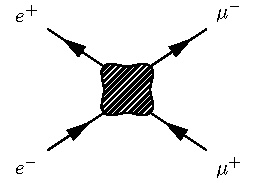
\includegraphics[width=0.30\textwidth]{feynmanDiagrams/output/ElElToMuMu}}}
            =
            \vcenter{\hbox{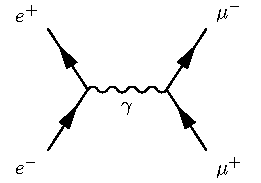
\includegraphics[width=0.25\textwidth]{feynmanDiagrams/output/ElElToMuMu_tree}}}
            +
            \vcenter{\hbox{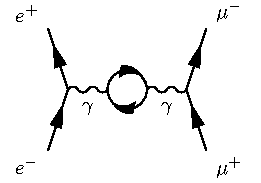
\includegraphics[width=0.25\textwidth]{feynmanDiagrams/output/ElElToMuMu_oneLoop1}}}
            \nonumber
            \\
            +
            \vcenter{\hbox{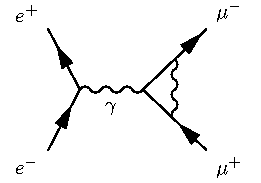
\includegraphics[width=0.25\textwidth]{feynmanDiagrams/output/ElElToMuMu_oneLoop2}}}
            +
            \vcenter{\hbox{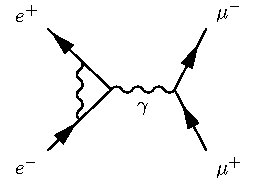
\includegraphics[width=0.25\textwidth]{feynmanDiagrams/output/ElElToMuMu_oneLoop3}}}
            +
            \vcenter{\hbox{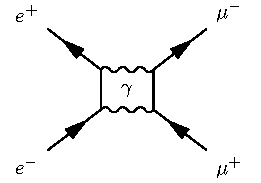
\includegraphics[width=0.25\textwidth]{feynmanDiagrams/output/ElElToMuMu_oneLoop4}}}
            +
            ...
            \nonumber
        }
        \caption{Illustration of development of the process $e^+ e^- \rightarrow \mu^+ \mu^-$
        in a model with only electrons and muons coupling to a photon. \label{fig:perturbativeDevelopment}}
    \end{figure}

    In this perspective, the parameters and the consistency of the Standard
    Model have been extensively measured and tested in several experiments, in particular
    at the LEP collider \cite{LEP}, the Belle and BaBar experiments \cite{BelleAndBabar}, and at the Tevatron collider \cite{Tevatron}. In 2012,
    the CMS and ATLAS experiments at the LHC discovered the last remaining particle of the
    Standard Model, the Higgs Boson with a mass $\mass{h} \sim 125\GeV$ \cite{CMSHiggs,ATLASHiggs}. The mass
    spectrum of the particles of the Standard Model is summarized on \reffig{fig:theory/fermionMasses} and
    shows a clear hierarchy between the different fermion generations.

    \reffig{fig:theory/standardModelFit} shows the result of a global fit of the electroweak
    Standard Model observables \cite{GFitter}. In such a procedure, the observables are
    fitted simultaneously according to the model, using as input the experimental measurements.
    After the fit, the resulting values for each observable ($O_\text{fit}$) are compared to
    the experimental measurement ($O_\text{meas.}$). The difference is finally compared to
    the experimental uncertainty ($\sigma_\text{meas.}$). This allows to have a global test of the consistency of
    the model, as any significant deviation between the predicted and measured values would
    indicate a flaw. The results shows that the theory is quite consistent, as no deviation
    larger than 3$\sigma$ is found.

    \insertFigure{theory/fermionMasses}{0.6}
                 {Masses of the fermions and bosons of the Standard Model. The photon
                 $\gamma$, gluon $g$ and neutrinos $\nu_\ell$ are not represented as they
                 are massless in the context of the Standard Model.}

    \insertFigure{theory/standardModelFit}{0.46}
                 {Global fit of observables of the electroweak Standard Model \cite{GFitter}.}

    \section{Shortcomings of the Standard Model \label{sec:standardModelShortcomings}}
    %====================================================================================

    Despite its success, the Standard Model contains theoretical open questions and unexplained
    experimental facts. For these reasons, it is considered as incomplete or as an effective
    theory valid only at low energy and hiding a larger theory at higher energy.
    In this section, we focus especially on the hierarchy problem and dark matter as they
    will be the most relevant one in the context of this document, and discuss briefly
    other open questions.

        \subsection{The hierarchy problem}

    The hierarchy problem is related to the corrections to the Higgs boson mass.
    To have a complete understanding of the problem, let's first look at the case of the
    mass of fermions and gauge bosons before looking at the Higgs \cite{SupersymmetryDemystified}.

    To compute a physical observable in a quantum field theory, one needs to
    integrate over all possible quantum corrections related to this parameter. In the case
    of the cross-section of a process, this means considering all loops and diagrams
    with the same initial and final states. For the mass of the mass of a particle, one is
    interested in diagrams that contribute to the propagator. An example of diagram contributing
    to the propagator of the electron is given in \reffig{fig:feynmanDiagrams/output/electronPropagator}. We may
    express the observable mass $m_e$ of the electron as the sum of the bare mass $m^0_{e}$,
    that is to say the actual parameter one writes in the Lagrangian, and $\Delta m_e$ representing
    the contributions from the quantum corrections:
    \eq{electronMassCorrection}
    {
        m^2_e \, = \, {m_e^0}^2 + \Delta m_e^2.
    }

    \insertFigure{feynmanDiagrams/output/electronPropagator}{0.4}
                 {Example of contribution to the electron propagator.}

    In effective theories, the computation of quantum corrections is done with respect to
    an energy cutoff $\Lambda$, representing the scale at which new physics is expected
    to play a significant role. In the case of \reffig{fig:feynmanDiagrams/output/electronPropagator},
    this means that we shall integrate over all momentum inside the loop, up to the scale $\Lambda$.
    For instance, if one considers electrodynamics as an effective theory of the electroweak
    symmetry, at one-loop level, the correction is given by:
    \eq{electronMassCorrection2}
    {
        \Delta m_e \, \simeq \, \frac{\alpha}{4\pi} \, m_e^0 \, \text{ln}\left(\frac{\Lambda}{m_e^0}\right).
    }

    With $\Lambda = \Lambda_{\text{electroweak}} = \orderOf{100\GeV}$, we find that
    $\frac{\Delta m_e}{m_e} \sim 20\%$. It is a relatively small correction, in the sense
    that it is not surprising to have a mass for the electron that is $\orderOf{1\GeV} \ll \Lambda_{\text{electroweak}}$.
    The most important feature in \refequation{eq:electronMassCorrection2} is the fact that $\Delta m_e$
    is proportional to $m_e^0$ and not $\Lambda$ as it means that the mass will not skyrocket
    as $\Lambda$ grows.

    There is a remarkable and more general property behind this term, which is that a
    gauge invariant Lagrangian cannot generate corrections that break the symmetry. In
    the case of electrodynamics with a massive electron, the mass term is already breaking
    the chiral symmetry $U(1)_L \times U(1)_R$, but because this is a so-called soft-breaking
    term (i.e. from spontaneous symmetry breaking), the property should still hold in
    the limit where $m_e^0 \rightarrow 0$. Therefore the correction cannot be proportional to
    $\Lambda$ but only to $m_e$, by dimensional analysis. It is common to refer to this by
    saying that chiral symmetry protects the mass of fermions from diverging. The same fact
    is observed for gauge bosons masses in the case of the electroweak symmetry breaking by
    the Higgs field: here, the gauge bosons are protected by the gauge invariance.

    Regarding the mass of the Higgs boson,  the Standard Model does not include
    any mechanism that prevents the mass of a scalar boson from diverging. The actual
    computation for the correction from a fermion loop gives:
    \eq{higgsMassCorrectionFromFermion}
    {
        \Delta m_h^2 \, \propto \, m_f^2 \Lambda^2,
    }
    which diverges with $\Lambda$. If one believes that the Standard Model is valid
    up to the Planck scale, where gravity is expected to play a significant role, then
    the observable Higgs mass can be written as
    \eq{higgsMassCorrectionTotal}
    {
        m_h^2 \, \simeq \, {m_h^0}^2 + \kappa \cdot m^2_\text{Planck}
    }
    where $\kappa$ is a function of the Standard Model parameters. The
    three quantities $m_h^0$, $\kappa$, and $m_\text{Planck}$ are \emph{a priori} unrelated
    to each other from the point of view of the theory. Hence, unless the parameters of the
    Standard Model conspire with each other and are \emph{fine-tuned} at twenty decimal
    places, there is no reason to expect that $m_h \ll m_\text{Planck}$. However, we observe
    that $m_h \sim \orderOf{10^2\GeV} \ll m_\text{Planck} \sim \orderOf{10^{19}\GeV}$, which
    is not natural. This is referred to as the hierarchy problem, as from these considerations
    there is no reason to expect such a large hierarchy between the electroweak scale and
    the Planck scale.

        \subsection{Dark matter}

    Dark matter is one of the greatest mystery in cosmology and fundamental physics at present time.
    The first observation leading to the dark matter hypothesis came from the measurement
    of rotation curves of galaxies \cite{Begeman}. These curves showed the evolution of
    the orbital velocity of stars inside galaxies as function of their distance to the
    galactic center. One can predict such curves by inferring the galaxy's mass repartition
    from models and spectrometry, and applying Newton's law of gravitation. The observed
    curves are well-described for the central region of the galaxy but then instead of
    decreasing with distance as predicted, were found to stay approximately constant.

    This observation suggested that there is a halo of invisible matter around
    galaxies, interacting gravitationally but not electromagnetically with the rest of the
    matter, hence the denomination of \emph{dark} matter. Further experimental measurements
    provided indirect evidences for the existence of such dark matter \cite{DMPrimer}.
    Among them, the technique of gravitational lensing allows the observer to
    infer the distribution of the mass inside a galaxy or a cluster from the bending of
    the light emitted by an object further in the background. Nowadays, dark matter is
    part of the standard model of cosmology as there are many astrophysical and cosmological
    phenomena which cannot be described without it, and has been found to represent
    $\orderOf{80\%}$ of the matter content of the universe.

    However the nature of dark matter is still unknown and it has not been directly observed.
    Dark matter candidates must be gravitationally interacting,
    not be short-lived and must not be baryonic. Last but not least, it must also be
    cold, meaning that it must have low kinetic energy, which rules out neutrinos
    as dark matter candidates \cite{NeutrinoNotDM}. It is now commonly admitted that there is no suitable
    candidate for it in the Standard Model.

    If one assumes that dark matter is made of a single particle $X$ thermally produced
    in the early universe, then it is possible, using the Boltzmann equation, to compute
    the relic density $\Omega_X$ \cite{DMPrimer, NeutralinoRelic, WIMPRelic}. This
    relic density is proportional to $m_X^2 / g^4_X$ where $m_X$ is the mass of the dark matter particle
    and $g_X$ is the coupling constant in the co-annihilation process $XX \leftrightarrow f\bar{f}$.
    It is remarkable to note that taking $\Omega_X = \orderOf{0.1}$ from cosmological
    observations and $g_X \sim 0.6$ from the weak interaction, we expect $m_X =
    \orderOf{100\GeV}$. This encourages physicists to look for weakly interacting massive
    particles (or WIMPs) which are predicted by many models beyond the Standard Model.

        \subsection{Other open questions and criticism}

    Other open questions or unexplained facts strengthen the belief that the Standard Model
    is not the final theory.

    \begin{itemize}
        \item \textbf{Dark energy} - The standard model of cosmology, so-called $\Lambda$CDM model,
            contains a non-zero cosmological constant $\Lambda$. The cosmological
            constant is initially an additional authorized term in Einstein's equation
            which relates space-time curvature to energy-momentum. Such term is necessary
            to explain the observed accelerated expansion of the universe from the study
            of the redshift of supernovas. The cosmological constant can be interpreted
            as vacuum energy, often referred to as dark energy. Despite the fact that this
            is in principle in agreement with quantum field theory which predicts vacuum
            energy from vacuum quantum fluctuations, there is a complete mismatch, of $\orderOf{10^{120}}$,
            between the small measured value of $\Lambda$ and its prediction
            by quantum field theory. This is often called the vacuum catastrophe or the worst
            prediction in the history of physics. A big challenge of current physics therefore
            consists in understanding the nature of dark energy and the reason why it is so small
            compared to predictions.
        \item \textbf{Matter-antimatter asymmetry} - It is a well established fact that
            the baryonic content of the Universe is made of matter. Because matter and antimatter
            should have been produced in equal proportion during the big bang, there must
            be sources of asymmetry that led to a state dominated by matter. Sakharov
            established a set of conditions that would
            induce such an asymmetry. Among them is the violation of the symmetries C (charge)
            and CP (charge-parity). The Standard Model
            with massless neutrinos contains two sources of CP-violation originating from
            the CKM matrix and the CP-violating phase in the QCD sector. So far however,
            these sources are not important enough to explain the magnitude of the baryon
            asymmetry.
        \item \textbf{Neutrino masses} - It has been measured by experiments that neutrinos
            can oscillate from one flavor to another. This indicates that neutrinos should
            be massive and have different flavor states than mass states much like down-type
            quarks and the CKM matrix. The problem of neutrinos being massive is itself not
            so much a problem as it is possible to introduce right-handed neutrinos in the
            field content of the Standard Model. However the exact mechanism depends on
            whether neutrinos are Dirac or Majorana fermions. The main source of interrogation
            is to understand why neutrinos have such a small mass compared to the other
            fermions.
        \item \textbf{Strong CP problem} - As introduced before, there is a term allowed in
            the QCD Lagrangian that introduces CP-violation via a phase $\theta$. The value
            of this parameter has been so far found to be very close to zero despite
            lack of theoretical arguments for it not to be of the order of 1. This situation
            is similar to the hierarchy problem for which we can expect that a
            hidden mechanism protects this phase to be too different from zero.
        \item \textbf{Quantum gravity description} - Gravitation is currently not described
            by the Standard Model. The underlying problem, which is to know how to unify general
            relativity with quantum field theory, is one of the biggest problem of modern
            physics. If it exists, the gauge boson associated to gravitation would
            need to have a spin equal to 2. It is however not known if and how such
            a theory would be renormalizable as it leads to uncancellable divergences.
        \item \textbf{Forces unification} - Several times in the history of physics,
            phenomenons have been understood to have a common structure and
            been unified. The simple name electromagnetism has in its etymology a clear
            reference to electrodynamic and magnetism. It is therefore natural for physicists
            to look for possibilities of unification, in our case regarding the electroweak
            and strong interaction, and ultimately with gravitation.
        \item \textbf{Free parameters and arbitrary field content} -
            Finally, there are conceptual interrogations about the fact that the quarks have
            such different masses, in particular regarding the top quark as it is the
            heaviest known particle. The same kind of conceptual interrogations goes about
            the number of fermion families: is there any fundamental reason to have three
            families instead of one, two, or an infinity of them? More generally, there
            are numerous facts about the Standard Model parameters and field content that
            feel arbitrary and may hide an underlying, more fundamental pattern.
    \end{itemize}


    \section{Theories beyond the Standard Model \label{sec:beyondTheStandardModel}}
    %====================================================================================

        \subsection{Zoology of Standard Model extensions}

        Since a few decades, extensions to the Standard Model have been proposed and
        studied with the aim to address its shortcomings. One can attempt to categorize
        them as function of the fundamental ingredients they add to the theory, either
        additional symmetries, space-time dimensions or field content.

            \subsubsection{Additional or extended symmetries}

        One of the possibility to extend the Standard Model is to look at symmetries.
        There are different kind of symmetries that can be considered, which do not impact the theory
        the same way, namely space-time symmetries or gauge symmetries. The only possible
        extension of space-time symmetries is supersymmetry which is discussed later
        in a dedicated section. For the moment, let us focus on additional or extended gauge
        symmetries.

        It is possible to think about gauge groups which include the Standard Model group,
        $SU(3) \times SU(2) \times U(1)$ to create Grand Unification Theories (GUT) in which
        the coupling constants are unified. Such groups are also motivated because they
        naturally introduce a symmetry between leptons and quarks as one can think of
        when looking at the pattern of the Standard Model.

        The most simple group one can find is $SU(5)$ \cite{SU5GUT} which would be a broken symmetry at
        low energy just as the electroweak symmetry is. Rotations in the $SU(5)$ space
        can mix the quark and lepton fields which led to a prediction of proton decay
        incompatible with experimental measurements. Grand-unification with $SU(5)$ is
        now mostly abandoned but remains an idea studied for larger groups such as $SO(10)$.

        On another side, driven this time by the strong CP problem,
        an idea introduced in 1977 \cite{PecceiQuinnAxion} consists in introducing a new
        global $U(1)$ symmetry with a new scalar field which breaks this symmetry, and
        ends up with a strong CP phase being naturally zero. This theory predicts a new
        particle, the axion, which turns out to be a good dark matter candidate.
        Axions would have masses lower than $\orderOf{1~\text{eV}}$ while still satisfying
        the criterion to be cold dark matter candidates. In particular, axions are predicted to
        form a Bose-Einstein condensate, which offers an opportunity to distinguish them
        from other dark matter candidates such as WIMPs \cite{AxionBoseEinstein}.

        \subsubsection{Additional dimensions}

        The second possibility is to add extra space-time dimensions. While everyday's life
        is only composed of 3+1 (space and time) dimensions, theoretical mechanisms can
        explain why additional dimensions are not noticeable at our scale.
        The extra dimensions are usually considered to be space-like dimensions, as an
        additional time-like dimension would break causality. Extra dimensions theories
        are of particular interest to unify interactions with gravitation and answering
        the hierarchy problem.

        A first idea is to consider extra dimensions that are compactified such that they
        are not noticeable at macroscopic scales. An useful analogy to understand the
        compactification concept is to consider that, for instance, a guitar string
        seen from very far looks like a one-dimensional object, whereas if one looks at it
        closely, it exhibits a second periodic dimension around the string axis because of its
        thickness. When adding such compactified, periodic dimension, one must therefore
        state the radius of this dimension, defining the compactification scale.

        Large extra dimensions (ADD) \cite{ADD} theories are based on the idea that the
        Standard Model interactions take place only in the four well-known dimensions and
        gravity would be allowed to travel extra, compactified dimensions. As a consequence,
        at large distances, gravity would be diluted while at low distances (i.e. high
        energies) the Standard Model interactions and gravitation would have coupling
        constants that are of the same order. A phenomenological consequence is that microscopic
        black holes could
        be produced in high-energy collisions provided that the collision probe distances
        lower than the Schwarzschild radius. Alternatively, universal extra dimensions
        (UED) \cite{UED} theories assume that all interactions may travel through the extra
        dimensions. Phenomenologically, one would observe in that case a discrete mass
        spectra for the Standard Model particles corresponding to excitations along the
        compactified dimensions.

        An other idea, found in Randall-Sundrum scenarios (RS) \cite{RS}, considers a five
        dimensions universe made of two four-dimension branes separated by an extremely
        warped fifth dimension. One of the brane corresponds to the Standard Model physics
        while the other brane would correspond to the realm of gravity. The distance
        separating the two branes is directly linked to the difference of energy scales
        between the Standard Model sector and the gravitation sector. A phenomenological
        prediction of these models is the production of graviton excitations at the TeV
        scale.

        \subsubsection{Additional or modified field content}

        A third possibility is to introduce new ad-hoc fields or modify existing ones
        to address the shortcomings of the Standard Model.

        One of the most obvious idea
        one can come up with is to postulate a fourth family of fermions. However, there are
        tight constraints on the existence of such a fourth family, starting with with
        limits on the number of neutrinos with a mass lower than $\mass{Z}/2$ from measurements
        of the branching ratio $\text{BR}(Z \rightarrow \text{invisible})$ \cite{PDFNumberOfNeutrinos}.

        Focusing on the problem of neutrino masses, some theories are being investigated,
        predicting the existence of sterile neutrinos or right-handed neutrinos \cite{RHNeutrinos}. Such neutrinos
        are expected to be heavy and would then be good dark matter candidates, and in some
        cases would explain why left-handed neutrinos have such a low mass, for instance
        in the context of the See-Saw mechanism \cite{Seesaw}.

        Alternatively, focusing exclusively on the dark matter problem, it has been proposed
        that dark matter is not made of just one, but several kind of particles regrouped
        in the concept of an hidden sector. There are several possibilities to describe
        the link between the Standard Model and this hidden sector, for instance by assuming
        that the Higgs boson relates the two sectors, or by introducing a new $U(1)_H$ gauge
        group whose gauge boson would be a ``dark'' photon \cite{darkPhoton}.

        Finally, one elegant idea to try to explain the lightness of the Higgs boson is to
        consider it as a composite object \cite{LittleHiggs, CompositeHiggs}. This idea is
        inspired from QCD where light scalars are encountered and do not exhibit a naturalness
        problem. Pions for example, in the massless quark limit, are massless Goldstone
        bosons coming from the breaking of the chiral symmetry by the QCD vacuum, composed
        of the chiral condensate $\left<\bar{q}_L q_R\right>$. However in practice,
        chiral symmetry is not exact as the quarks are massive, and thus pions are only
        pseudo-Goldstone boson and get a mass - though they are still protected from being
        heavy by the approximate chiral symmetry. This idea can be applied to the Higgs,
        which would be a Goldstone boson of a new strongly-interacting sector above the
        weak scale, and would solve the hierarchy problem. Phenomenologically, different
        signatures exist depending on the exact model considered, but can involve different
        couplings to gauge bosons compared to the Standard Model, and the existence of new
        particles such as top partners.

            \subsubsection{The anthropic principle}

        Finally, one of the alternative to theories beyond the Standard Model is to
        simply accept the Standard Model as it is. This is strongly related to Einstein's
        interrogation regarding whether or not Nature had any choice at the creation of
        the universe. It can be argued that most of the shortcomings of the Standard Model
        are related to gravitation and cosmology and might simply be unsolvable at scales accessible
        by particle physics experiments. The most important remaining issues are related to
        fine-tunning in the hierarchy problem and the arbitrariness of the other parameters
        of the theory.

        The anthropic principle states that when studying the universe, it should be taken
        into account that it allows for conscious life to exist. It might be that our universe
        is simply one realization of universe among many others in what would be called a
        multiverse. What appears to be fine-tunning would in fact be equivalent to natural
        selection at the scale of the multiverse where the observed universes can only be
        the ones allowing conscious life \cite{AnthropicPrincipleBarrow, StarsInOtherUniverses}.

        This view is however controversial, as it is not clear at this point what kind of
        testable prediction such an idea can provide. It nevertheless remains a legitimate
        hypothesis and questions the place and origin of the universe. A more extensive
        and interesting discussion can be found in \cite{MultiversBarrau}.

        \subsection{Supersymmetry \label{sec:SUSY}}

        \subsubsection{General idea and motivations}

        Here, we propose to have a dedicated look at the idea of supersymmetry. Supersymmetry
        (SUSY), emerged around the 70's. At this time, Gol'fand and Likhtman, two
        russian mathematicians, were working with the space-time symmetries of the Poincaré
        group. The usual space-time symmetries, i.e. translations, boosts and rotations,
        are all bosonic symmetries. They noticed that another type of space-time symmetry
        with fermionic (i.e. spin 1/2) generators could also exist \cite{FirstSUSYPaper}.
        Such a symmetry $Q$,
        the supersymmetry, would therefore relate the different representations of the
        Lorentz group, namely fermions ($f$) and bosons ($b$):
        \eqalign{SUSYtransformation}
        {
            Q \rvert \text{f} \rangle \rightarrow \rvert \text{b} \rangle \nonumber
            \\
            Q \rvert \text{b} \rangle \rightarrow \rvert \text{f} \rangle.
        }
        $Q$ is therefore a non-trivial extension of the
        Poincaré algebra. This is an important consideration: it has been demonstrated by
        Colemand and Mandula \cite{ColemandMandula} that the only possible symmetries of Nature are the
        Poincaré symmetry and the gauge symmetries. Nevertheless, Haag, Lopuszanski and
        Sohnius later relaxed this theorem \cite{HaagLopuszanskiSohnius} by noticing that another type of symmetry is
        possible and precisely corresponds to supersymmetry \cite{SUSYPrimer, Dawson}.

        Here, we have introduced $Q$ as a \emph{global} symmetry, i.e. a transformation
        that does not depend on space-time, and is therefore not a gauge symmetry.
        However, a remarkable feature in SUSY is that trying to gauge $Q$, meaning making
        the transformation space-time dependent, yields a description of gravitation called
        supergravity (SUGRA). Supersymmetry also provides a link with string theory which
        is a candidate for the « theory of everything\, ».

        To each fermion is therefore associated a boson with same quantum numbers (apart
        from spin), and similarly to each boson
        is associated a fermion. The particle associated to another one by SUSY is called
        its superpartner, and can be put together in a superfield. To ensure the consistency
        of the theory, superpartners of vector bosons have spin 1/2 and superpartners
        of fermions have spin 0. SUSY alone predicts that a particle and its superpartner
        should have the same mass. However this cannot be the case in practice as no
        such thing has been observed by experiments, meaning that supersymmetry must be
        a broken symmetry.

        There are several mechanisms that are candidates to spontaneously break SUSY. Some
        are based on a gravity mediated supersymmetry breaking (such as minimal SUGRA),
        others involve a gauge mediated mechanism (GMSB), and another possibility is to
        have an anomaly mediated breaking (AMSB). Since the exact mechanism is unknown at
        the moment, one solution is to simply add a $\mathcal{L}_\text{soft}$ component to
        the Lagrangian, that includes all allowed terms and corresponding new parameters.

        One of the main motivations for supersymmetry is to provide a mechanism that
        protects the mass of scalar bosons, thus answering the hierarchy problem. In the
        case of the Higgs boson, one can show
        that if the superpartners have equal masses, then the quadratic divergences
        introduced in \refequation{eq:higgsMassCorrectionFromFermion} cancel each other and
        it becomes natural for the Higgs boson to have a mass much lower than the Planck scale.
        If SUSY is only softly broken (i.e. broken spontaneously), as for chiral and gauge
        symmetries, then the boson-fermion symmetry still prevents to have a quadratic
        divergence. Instead, we are left with a mild logarithmic divergence:
        \eq{higgsMassCorrectionInSUSY}
        {
            \Delta m_h^2 \, \propto \, (m_f^2 - m_b^2) \, \text{ln}\left(\frac{\Lambda}{m_b}\right).
        }
        But this alone does not solves everything. If one consider the most massive
        fermion, i.e. the top quark $t$, then the mass ratio with its superpartner the
        stop $\tilde{t}$, $r = m_{\tilde{t}} / m_t$ cannot be too large. For instance,
        we assuming $r = 100$, then we are left with a correction $\Delta m_h = \orderOf{100 \cdot m_t}$
        which is still large considering as we seek $\orderOf{m_h} = \orderOf{m_t}$.
        Therefore, we would need to reintroduce a certain level of fine-tunning in the
        parameters of the theory for the corrections to cancel each others, and we want
        to avoid that in order to keep the theory natural. Hence, the naturalness of SUSY
        is strongly related to the mass of the superpartners, and can be used as an indication
        for experimental searches.

        \subsubsection{The MSSM}

        The most studied realization of supersymmetry is the Minimal Supersymmetric Standard
        Model (MSSM), corresponding to adding the minimum number of fields to the Standard
        Model for it to become supersymmetric \cite{Dawson, Vempati, Romao}.
        Since the MSSM breaks SUSY with ad-hoc terms, it is to be seen as an effective
        theory up to $\Lambda_{\text{SUSY breaking}}$.

        At each fermion and gauge boson is therefore associated a superpartner that we may
        call sfermion and gaugino. It should be
        stressed once again that left-handed and right-handed fermions are different
        fermions. Hence, there are for example two selectrons, one associated to
        each chirality of the electron. These are usually noted $\tilde{e}_R$ and $\tilde{e}_L$
        to associate them easily with their fermion partner, even though they are spinless.
        Regarding the Higgs sector, it is necessary to add not only a superpartner called
        higgsino, but a second Higgs $SU(2)$ doublet to avoid a gauge anomaly.

        As shown in the case of the Standard Model, the mass eigenstates are not
        necessarily the flavor eigenstates. This is still true in the MSSM, especially
        because of the SUSY breaking terms, and is an important consideration for the
        phenomenology. The introduction of a second Higgs $SU(2)$ doublet leads to four
        additional physical Higgs states noted $H^0$, $A$ and $H^\pm$.
        In the supersymmetric sector, mass eigenstates are formed by the combinations of
        the higgsinos and electroweak gauginos and are called charginos $\tilde{\chi}^\pm$
        and neutralinos $\tilde{\chi}^0$.
        For the fermions, mixing terms are authorized in $\mathcal{L}_\text{soft}$ between
        the left and right-handed superpartners and are especially important for the
        phenomenology of the third generation. The mass eigenstates can be determined
        by diagonalizing the mass matrices. The resulting particles spectrum is given on
        \reftab{tab:MSSMsuperpartners}.

        \begin{table}
            \centering
            \begin{tabular}{ccc}
                \textbf{Flavor eigenstates} & & \textbf{Mass eigenstates} \\
                                            & & \\
            \begin{tabular}{|ccc|}
                \hline
                1$^\text{st}$ gen. & 2$^\text{nd}$ gen. & 3$^\text{rd}$ gen. \\
                \hline
                \hline
                $\tilde{u}_L$        &   $\tilde{s}_L$      & $\tilde{t}_L$ \\
                $\tilde{u}_R$        &   $\tilde{s}_R$      & $\tilde{t}_R$ \\
                $\tilde{d}_L$        &   $\tilde{c}_L$      & $\tilde{b}_L$ \\
                $\tilde{d}_R$        &   $\tilde{c}_R$      & $\tilde{b}_R$ \\
                \hline
                \hline
                $\tilde{\nu}_e$      &   $\tilde{\nu}_\mu$  & $\tilde{\nu}_\tau$ \\
                $\tilde{e}_L$        &   $\tilde{\mu}_L$    & $\tilde{\tau}_L$   \\
                $\tilde{e}_R$        &   $\tilde{\mu}_R$    & $\tilde{\tau}_R$   \\
                \hline
            \end{tabular}
            &
            &
             \begin{tabular}{|ccc|}
                \hline
                1$^\text{st}$ gen. & 2$^\text{nd}$ gen. & 3$^\text{rd}$ gen. \\
                \hline
                \hline
                "       &  " & $\tilde{t}_1$ \\
                "       &  " & $\tilde{t}_2$ \\
                "       &  " & $\tilde{b}_1$ \\
                "       &  " & $\tilde{b}_2$ \\
                \hline
                \hline
                "       &  " & "                  \\
                "       &  " & $\tilde{\tau}_1$   \\
                "       &  " & $\tilde{\tau}_2$   \\
                \hline
            \end{tabular}
            \\
            & $\rightarrow$ & \\
            \begin{tabular}{|ccc|}
                \hline
                Higgs   & Electroweak         & Strong          \\
                sector  & sector              & sector          \\
                \hline
                \hline
                $\begin{matrix} \tilde{h}^0_u, \tilde{h}^+_u \\ \tilde{h}^0_d, \tilde{h}^-_d \end{matrix}$
                &
                $\begin{matrix} \tilde{B} \\ \tilde{W}_{1,2,3}\end{matrix}$
                &
                $\begin{matrix} \tilde{g}_{1..8} \end{matrix}$ \\
                \hline
            \end{tabular}
            & &
            \begin{tabular}{|cc|}
                \hline
                Charginos and   & Strong          \\
                neutralinos     & sector          \\
                \hline
                \hline
                $\begin{matrix} \tilde{\chi}^\pm_{1,2} \\ \tilde{\chi}^0_{1,2,3,4} \end{matrix}$
                &
                "
                \\
                \hline
            \end{tabular}
            \end{tabular}
            \caption{Superpartners of the fermions and bosons of the Standard Model,
            categorized according to flavor eigenstates (on the left) and mass eigenstates
            (on the right). A symbol " indicates that the mass eigenstate is identical to
            the flavor eigenstate. \label{tab:MSSMsuperpartners}}
        \end{table}

        By design, the MSSM conserves a quantum number called R-parity defined as:
        \eq{RparityDefinition}
        {
            R = (-1)^{2S + 3B + L}.
        }
        where $S$ is the spin, $B$ the baryon number, and $L$ is the lepton number. $R$ is
        equal to 1 for the particles of the Standard Model and -1 for their superpartners.
        As it is conserved, supersymmetric particles can only be
        pair-produced and only decay into an odd number of supersymmetric particles. In
        particular, this means that the lightest supersymmetric particle (LSP) is stable as
        its decay would violate the $R$-parity. The important consequence is that it provides
        a good candidate for dark matter, provided that this particle is neutral.

        The construction of the MSSM leads to the introduction of more than 100 additional
        parameters compared to the Standard Model, with more than 50 coming from $\mathcal{L}_\text{soft}$.
        Dealing with such a large number of
        parameters is quite inconvenient in terms of phenomenological and experimental analysis.
        The phenomenological MSSM (pMSSM) reduces this number of parameters by assuming that
        there is no new source of CP violation, that the lightest neutralino $\lneutralino$
        is the LSP, and other assumptions on the sfermion masses, trilinear couplings and
        flavor violation. This reduces the number of new parameters to 19, namely:
        \begin{itemize}
            \item the higgsino mass parameter $\mu$ and pseudo-scalar Higgs mass $\mass{A}$ ;
            \item the ratio of the Higgs vacuum expectation values, $\text{tan}\, \beta \definedAs v_2 / v_1$ (with $0 \leq \beta \leq \frac{\pi}{2}$) ;
            \item the soft gaugino masses $M_1$, $M_2$ and $M_3$, corresponding respectively\footnote{One can notice that the index in $M_{1,2,3}$ refers to the gauge groups $U(1)$, $SU(2)$ and $SU(3)$, which makes it easier to remember which gaugino it refers to.} to the bino $\tilde{B}$, wino $\tilde{W}$ and gluino $\tilde{g}$ masses ;
            \item the first and second generation sfermion masses $\masstilde{\tilde{q}}$, $\masstilde{\tilde{u}}$, $\masstilde{\tilde{d}}$, $\masstilde{\tilde{l}}$ an $\masstilde{\tilde{e}}$ ;
            \item the third generation sfermion masses $\masstilde{\tilde{Q}}$, $\masstilde{\tilde{t}}$, $\masstilde{\tilde{b}}$, $\masstilde{\tilde{L}}$ and $\masstilde{\tilde{\tau}}$ ;
            \item the trilinear couplings $A_t$, $A_b$ and $A_\tau$.
        \end{itemize}
        Note that we wrote $\masstilde{}$ instead of simply $\mass{}$ to highlight that these
        masses comes from the SUSY breaking Lagrangian $\mathcal{L}_\text{soft}$ and not
        from the electroweak symmetry breaking.
        One can go one step further and reduce this number of parameters to 5 in the case
        of the constrained MSSM, noted cMSSM (or mSUGRA), by assuming that at grand unification scale, all the
        scalar particles have the same mass $m_0$, all gauginos have the same mass $m_{1/2}$,
        and all the trilinear couplings are equal to $A_0$. The remaining
        two parameters are $\text{tan}$ and the sign of $\mu$. Although the assumptions
        of the pMSSM and cMSSM can be seen as arbitrary, one can also simply take them as
        guidance to reduce the parameter space in the context of  phenomenology and
        experimental studies.

        \subsubsection{Phenomenology of the chargino, neutralino and stop sector \label{sec:stopNeutralinoCharginoPheno}}

        To get a better and concrete idea of the phenomenology of the chargino, neutralino
        and stop sector, which is of interest in this document, let's write down explicitly
        the mass matrices in the context of the MSSM and briefly discuss their implications.
        By mass matrices, we refer to the same kind of matrices that arose when we described
        the electroweak symmetry breaking in \refsection{sec:spontanneousElectroweakSymmetryBreaking}
        and which led to the introduction of the physical states $W^\pm$, $Z$ and $\gamma$.

        The chargino sector arises from the mixing between the winos $\tilde{W}_i$ and charged
        higgsinos $\tilde{h}^\pm$. In the ($\tilde{W}^\pm$, $\tilde{h}^\pm$) basis,
        the mass matrix is
        \eq{charginoMixingMatrix}
        {
            \mathcal{M}_{\tilde{\chi}^\pm}
            =
            \begin{pmatrix}
                M_2
                &
                \sqrt{2} m_W \,\text{sin}\, \beta
                \\
                \sqrt{2} m_W \,\text{cos}\, \beta
                &
                -\mu
            \end{pmatrix}
        }
        and the mass of the charginos $\tilde{\chi}_{1,2}^\pm$ are obtained by diagonalizing
        this matrix. The chargino sector is therefore only described by $M_2$,
        $\beta$ and $\mu$. For very large values of $\text{tan}\, \beta$, it is straightforward
        to see that the mass of the charginos tends to $M_2$ and $\mu$.

        The neutralino sector arises from mixing between the bino $\tilde{B}$, the wino
        $\tilde{W}^3$ and the two neutral higgsinos $\tilde{h}^0_1$ and $\tilde{h}^0_2$.
        In the corresponding basis, ($\tilde{B}$,$\tilde{W}^3$, $\tilde{h}^0_1$, $\tilde{h}^0_2$),
        the mass matrix is
        \eq{neutralinoMixingMatrix}
        {
            \mathcal{M}_{\tilde{\chi}^0}
            =
            \begin{pmatrix}
                M_1 & 0                     & - m_Z \,\text{cos}\, \beta \,\text{sin}\, \theta_W &   m_Z \,\text{sin}\, \beta \,\text{sin}\, \theta_W
                \\
                0   & M_2                   &    m_Z \,\text{cos}\, \beta \,\text{cos}\, \theta_W & - m_Z \,\text{sin}\, \beta \,\text{cos}\, \theta_W
                \\
                - m_Z \,\text{cos}\, \beta \,\text{sin}\, \theta_W  &   m_Z \,\text{cos}\, \beta \,\text{sin}\, \theta_W & 0 & \mu
                \\
                  m_Z \,\text{sin}\, \beta \,\text{sin}\, \theta_W  & - m_Z \,\text{sin}\, \beta \,\text{cos}\, \theta_W & \mu & 0
            \end{pmatrix}
        }
        where $\theta_W$ is the weak mixing angle. The neutralino masses therefore only
        depend on $M_1$, $M_2$, $\beta$ and $\mu$.
        For example, for $M_1$ and $M_2 \gg \mu$, the two lightest
        neutralinos are essentially higgsino-like.

        Finally, in the stop sector, $\tilde{t}_L$ and $\tilde{t}_R$ are not necessarily
        the mass eigenstates, noted $\tilde{t}_1$ and $\tilde{t}_2$. They are determined
        from the mass matrix
        \eq{stopMixingMatrix}
        {
            \mathcal{M}_{\tilde{t}}
            =
            \begin{pmatrix}
                \masstilde{{\tilde{t}_L}}^2 + m^2_t + m^2_Z(\frac{1}{2} - \frac{2}{3} \,\text{sin}^2 \theta_W) \,\text{cos}\, 2\beta
                &
                m_t ( A_{t} + \mu \,\text{cot}\, \beta)
                \\
                m_t ( A_{t} + \mu \,\text{cot}\, \beta)
                &
                \masstilde{\tilde{t}_R}^2 + m^2_t + \frac{2}{3} m^2_Z \,\text{sin}^2 \theta_W \,\text{cos}\, 2 \beta
            \end{pmatrix}
        }
        where $A_{t}$ characterizes the trilinear coupling appearing in $\mathcal{L}_\text{soft}$
        and $\masstilde{\tilde{t}_{L,R}}$ are the soft stop masses.
        The mixing between $\tilde{t}_L$ and $\tilde{t}_R$ is characterized by the off-diagonal
        terms and it is usually convenient to introduce the stop mixing parameter
        $X_t \definedAs ( A_{t} + \mu \,\text{cot}\, \beta)$.


%==============================================================
\setcounter{mtc}{3}
\chapterwithnum{The Compact Muon Solenoid experiment at the LHC}
\vspace*{-0.7cm}
\hspace*{0.39\textwidth}
\begin{minipage}{0.6\textwidth}
\emph{« Tracked you down with this. This is my timey-wimey detector. It goes ding when there’s stuff! »}\\
\hspace*{0.6\textwidth} The Tenth Doctor
\end{minipage}
\minitoc
\newpage
%==============================================================

    In this chapter, we introduce the Large Hadron Collider (LHC) and the Compact Muon Solenoid
    Experiment (CMS). In \refsection{sec:LHCintro}, we present the LHC apparatus,
    its scientific motivation and the physics of proton-proton collisions. In \refsection{sec:CMSexperiment},
    we describe the CMS experiment by describing the layout and technologies used for each
    subdetectors, as well as their performances. We will also go through the main techniques
    used to reconstruct the objects produced in the collisions. Finally in \refsection{sec:simu},
    we describe the principles behind the production of Monte-Carlo events, in particular
    the Monte-Carlo generation of collisions, the hadronization and the detector simulation.

    \section{The Large Hadron Collider \label{sec:LHCintro}}

    \subsection{Scientific context and challenges}

    There are several approaches one can follow toward new physics. For instance, using
     measurements of observables and exploiting the fact described in
    \refsection{sec:standardModelSuccess} that observables are impacted through loops by
    the entire Nature's Lagrangian, it is possible to infer information or limits regarding
    yet-unknown physics. Historically, this has been proved to be successful numerous times,
    for instance to predict the mass of the top quark from the $W$ and $Z$ bosons mass
    measurements \cite{discoveryOfTopQuark}. Similarly, a smoking-gun for some supersymmetric
    models is the enhancement of the branching ratio BR($B_s \rightarrow \mu^+\mu^-$)
    \cite{BsToMuMu}. However,
    despite the fact this approach provides valuable information, it can be criticized as
    only providing indirect evidences and not a clear window to new phenomena. Moreover,
    the statistics and detector resolution required to increase the accuracy of the
    prediction grow drastically.

    Another approach, probably the most attractive and informative, is the direct production and observation of
    new phenomena. One often forgotten fact is that new physics might not appear at high
    energies but at low energies instead. This is motivated for instance by axions
    theories and some hidden sector theories which predict particles with sub-eV masses
    or rare interactions \cite{PolarizedHelium, CavityForHiddenPhotons}. Nevertheless, it
    is more common to assume that new physics will show up at high energies. To probe
    higher energies, particle colliders have been
    built with increasing center of mass energies ($\sqrt{s}$) during the last decades.
    Two famous ones are the Large Electron-Positron (LEP) collider \cite{LEP} and the
    Tevatron collider \cite{Tevatron}. The
    LEP was an $e^+e^-$ collider which operated at a maximum of $\sqrt{s} \approx 200\GeV$
    at CERN in the 90's and allowed precise measurements of the electroweak $Z$ and $W$
    bosons and tested the robustness of the Standard Model. The Tevatron was a $p\bar{p}$
    collider which operated at a maximum $\sqrt{s} \approx 2\TeV$ at Fermilab until 2011
    and led to the discovery of the top quark and first measurements of its properties.
    Nowadays, the only high energy collider in operation is the Large Hadron Collider
    at CERN.

    The LHC \cite{LHC} is a circular hadron collider built at CERN, near Geneva. One of its physics
    goals is the production of high-energy proton-proton ($pp$) collisions to uncover the mechanism
    of electroweak symmetry breaking, to test the validity of the Standard Model, and more
    generally to explore physics around $0.1 \sim 10\TeV$ and possibly discover new
    physics. It is also capable of producing heavy ions (PbPb) collisions or proton-ion
    collision ($p$Pb) in order to study quark matter at high temperature,
    and in particular the properties of quark-gluon plasma. The rest of this document will
    focus on $pp$ collisions.

    The LHC collider has been built in the same tunnel as the LEP. The beam energy at
    the LEP was largely limited by the energy loss from synchrotron radiation. This loss
    is proportional to $E^4 / (m^{4} r^{2})$ with $E$ and $m$ being the energy and mass of the
    particle, and $r$ the radius of the tunnel. As $m_p$ is much larger than $m_e$, it is
    easier to maintain the energy of a rotating proton beam than an electron/positron one.
    Consequently, using protons is preferred in the context of reaching the highest possible
    energy, justifying this choice for the LHC. We will see however, in
    \refsection{sec:physicsFromCollisionsAtTheLHC}, how proton collisions are more challenging
    from the point of view of the reconstruction and analysis due to their internal structure.

    \subsection{Beam injection, control and acceleration}

    The creation and first acceleration of the proton beam work as follow. Protons are initially
    obtained by heating low-pressure $H_2$ gas which produces $H^+ (= p)$ and $e^-$, and
    by isolating the protons using high voltages. The protons are fed to an acceleration
    chain made of consecutive accelerators which use radio frequencies to create an acceleration
    gradient. At the end of the chain, in the Super Proton Synchrotron (SPS), the
    beam acquires an energy of $450\GeV$ before being injected in the LHC ring. The LHC
    ring is a tunnel of 27 kilometers built between $50$ and $200$~m underground. The
    project was originally designed to accelerate the proton beam up to $7\TeV$ per beam,
    corresponding to a center of mass energy $\sqrt{s} = 14\TeV$. Four main experiments are
    installed along the ring, at each collision point. Two of them, ATLAS and CMS, are
    general-purpose experiments while ALICE focuses on heavy-ion collisions, and LHCb studies
    $B$ and $C$-hadrons properties and $CP$-violation. \reffig{fig:LHClayout} presents an
    overview and the general layout of the machine.

    \insertTwoFigures{LHClayout}
                     {LHC/LHCring}
                     {LHC/LHClayout}
                     {0.6}
                     {On the top, sketch of the underground installation showing the SPS,
                     the injection tunnels, the LHC, as well as the four experiments. On
                     the bottom, layout of the LHC ring. The installation is divided in
                     eight octants, with some of them dedicated to collisions but also
                     injection, acceleration (RF) and beam dump.}

    One of the biggest challenges of the LHC was the design and operation of magnets
    powerful enough to bend the trajectory of the protons at such high energies. To do
    so, superconducting magnets made of a niobium-titanium alloy are used and are able to
    produce a magnetic field of up to $8.33~\text{T}$. The operating temperature of such magnets
    is only a few Kelvins: in the context of the LHC, they are required to be cooled using
    a complex system of superfluid $^4$He at $1.9~\text{K}$. It is remarkable to note that this
    temperature is actually cooler than the cosmic microwave background at around $2.7~\text{K}$.

    Operating superconducting magnets requires a good control and understanding of quenches.
    A magnet quench occurs when a part of the superconducting material looses its superconducting
    property and starts to heat because of Joule effect. Because the critical temperature
    is usually low, this can create a chain reaction as the heat spreads. Quenches are
    not such unusual events, and the LHC employs a sophisticated system to detect them and protect
    the magnetic system by automatically dumping the beam, mitigating the effect of the
    quench and extracting the energy stored inside the magnet \cite{LHCmagnets}.
    However, defects in the protection
    system or more generally in the electrical and mechanical apparatus can have dramatic
    impact as the energy can easily damage the machine if improperly released. In 2008,
    a faulty electrical interconnection between two magnets led to an electrical arc that
    punctured the cryogenic fluid enclosure and vaporized a fraction of the fluid, causing
    important damages to the installation \cite{LHCindicent}.

    The pipes of the LHC consist of about 1200 dipole sections represented on
    \reffig{fig:LHCpipe}, each $15$ m long, whose role are to bend the beam using dipole
    magnets. In addition, about 400 quadrupole magnets are used to squeeze the
    beam. Higher multipolar magnets are also used to prevent and correct instabilities of
    the beam. The effective bending radius, created from the $17.6$ km of dipoles, is
    $r \approx 2.8$ km, to be compared to the radius of the full apparatus being about $4.3~\text{km}$.

    \insertTwoFigures{LHCpipe}
                     {LHC/dipoleCrossSection2}
                     {LHC/pipePhoto2}
                     {0.7}
                     {On the top, cross-section of a cryodipole of the LHC
                     showing the magnet coils around the two beam pipes, and the cooling system \cite{LHC}.
                     On the bottom, technician working on an interconnection between two LHC
                     sections (credits: Anna Pantelia, CERN).}

    Each beam is organized in bunches of protons separated by a time interval of 50 or
    25~ns depending on the machine configuration. Each bunch is made of about $10^{11}$
    protons. The LHC uses radio frequency cavities to increase the energy of the beam by
    about 0.5 MeV per rotation, or $5.4\GeV$ per second. At $7\TeV$ per beam with 25 ns
    between bunches, the total energy of the beam is about 360 MJ and the energy stored
    in the magnet system is about 600 MJ, roughly corresponding to the energy of a
    lightning bolt. The beams are then made to collide at four different points along the
    ring, corresponding to the four main experiments.

        \subsection{Physics of $pp$ collisions \label{sec:physicsFromCollisionsAtTheLHC}}

    When considering a single $pp$ collision, it must be kept in mind that protons are
    composite objects made of three valence quarks in a sea of virtual partons, i.e.
    virtual quarks and gluons. At a given moment, partons in the proton only carries a fraction
    of the total proton momentum. Because of the properties of quantum chromodynamic, the
    structure of the proton can not easily be derived from first principles given our current
    capabilities. Instead, we must rely on the parton distribution functions (PDF), determined
    from experiment, characterizing the probably to find a parton with a fraction of
    momentum $x$, depending on its nature. Two examples of PDF are given on
    \reffig{fig:partonDistributionFunctionsExample}. The shape of these
    distributions implies that, in a collision, the center of mass energy of the two incoming
    partons is generally much lower than the beam energy.  Each incoming parton may also
    radiate partons right before the interaction, a process called initial state radiation
    (ISR), leading to additional jets in the event. Similarly, radiations from quarks or
    gluons in the final state are called final state radiation (FSR). Finally, the remaining
    partons from the protons may interact with each other in what is called the underlying
    event, and produce high-energy forward jets, almost collinear to the beam axis. $pp$
    collisions are therefore complex processes, as summarized in \reffig{fig:LHC/ppCollision},
    due to the composite nature of the proton and the fact that the partons are colored
    objects.

    \insertFigure{partonDistributionFunctionsExample}{0.85}{Example of PDFs
    for two different energy scales $Q$, provided by the MSTW group \cite{MSTWpdfs}. At lower energies,
    one clearly distinguish the large fraction of momentum $x$ carried by $u$ and $d$ valence
    quarks while other species are only present in the parton sea and less probable as
    their mass increases. As $Q^2$ grows, the probability to probe sea partons increases. }

    \insertFigure{LHC/ppCollision}{0.7}{Feynman diagram showing the complexity of a
    single proton-proton collision. Two partons from the incoming protons participate
    to the hard scattering leading to a $Z/\gamma^*$ resonance which decays into two
    quarks. In both the initial and final states, the colored particles may radiate gluons
    (or a gluon may split into a quark pair), leading to initial and final state radiations.}

    In the context of the LHC, the number of $pp$ collisions happening per unit of time is
    proportional to the instantaneous luminosity $L_\text{inst.}$ which depends on the bunch crossing
    frequency, the number of bunches, the number of proton per bunches and other beam and
    geometry parameters. The two general purpose experiments, ATLAS and CMS, are designed
    for a typical luminosity $L_\text{inst.} = 10^{34}~\text{cm}^{-2}
    \text{s}^{-1} = 10~\text{nb}^{-1} / \text{s}$. For a given process, one can compute $n$
    the number of expected events per unit of time:
    \eq{numberOfEventInst}
    {
        n & = L_\text{inst.} \times \sigma_\text{process} \\
    }
    where $\sigma_\text{process}$ is the cross-section of the process considered. Later, we may refer
    to the integrated luminosity $L_\text{integr.}$ over a defined period of data-taking,
    which relates to $N$, the total number of expected events during that time:
    \eq{totalNumberOfEvents}
    {
        N & = L_\text{integr.} \times \sigma_\text{process}
    }

    \reffig{fig:LHC/ppCrossSections} shows the evolution of the cross section of different
    processes such as $W$, $Z$, top or Higgs production as function of $\sqrt{s}$. The
    total inelastic cross section is about 60~mb. At an instantaneous luminosity of
    $10~\text{nb}^{-1} / \text{s}$ and with a bunch crossing every 25~ns, this corresponds
    to an average of 15 inelastic interactions per bunch crossing. This is what is behind
    the notion of pile-up: one event, or bunch crossing, contains $\orderOf{10-30}$ interactions
    with generally at most one of interest, e.g. the production of a $W$ or $Z$ boson.

    \insertFigure{LHC/ppCrossSections}{0.6}{Evolution of the cross sections of typical
    processes for $p\bar{p}$/$pp$ collisions as function of $\sqrt{s}$. Two vertical
    lines corresponds to the center of mass energy of the Tevatron ($\sqrt{s} \approx 2\TeV$)
    and the LHC ($\sqrt{s} =$ 7, 8 and 14$\TeV$) \cite{ppCrossSectionsStirling}.}

    The concept of pile-up have crucial implications for the study of $pp$ collisions: the
    additional inelastic hadron collisions naturally produce jets of particles, which
    pollute the environment of each event, affecting the number of hits in the tracking
    detectors and the energy measurement in calorimeters. It is thus needed to develop
    methods to mitigate the effect of pile-up.

    \subsection{LHC timeline and roadmap}

    \reftab{tab:LHCtimeline} presents the timeline and roadmap of the LHC. Because of the
    incident that happened in 2008, the machine had to be repaired and collisions could
    only be provided at energies $\sqrt{s} = 7$ and $8\TeV$ during the Run I, while waiting for consolidations
    of the machine. An integrated luminosity of respectively $5$ and $20\invfb$ was recorded
    at these energies. During 2015 and until the end of 2018, the LHC is expected to work
    at $13$ or $14\TeV$ and to provide about $100\invfb$ of integrated luminosity. After
    the run III, foreseen to take place from 2021 and to the end of 2023, the LHC is expected to be upgraded,
    which would be the start of the high-luminosity LHC (HL-LHC) program. During this period,
    the LHC will still operate at $14\TeV$ but with an instantaneous luminosity around
    100$~\text{nb}^{-1} / \text{s}$ corresponding to a pile-up around 150. To be able to
    sustain such conditions, the LHC experiments will need to be significantly upgraded.

    \begin{table}[h]
        \begin{tabular}{|c|c|c|c|c|c|c|}
            \hline
            & Period
            & $\sqrt{s}$ (TeV)
            & $<$Pile-up$>$
            & $L_{inst.}$ ($\text{nb}^{-1} / \text{s}$)
            & $L_{integr.}$ (fb$^{-1}$) \\
            \hline
            Phase 0, Run I    & 2010-12 & 7-8   & 20      & 6-7   & 5+20\\
            \hline
            \hline
            Phase 1, Run II   & 2015-18 & 13-14 & 40      & 15    & 100\\
            Phase 1, Run III  & 2021-23 & 14    & 60      & 20-30 & 300\\
            \hline
            \hline
            Phase 2 (HL-LHC)  & 2027    & 14    & 130-200 & 100   & 3000\\
            \hline
        \end{tabular}
        \caption{Timeline and roadmap of the LHC (as of July 2015).\label{tab:LHCtimeline}}
    \end{table}

    \section{The Compact Muon Solenoid experiment \label{sec:CMSexperiment}}

    The Compact Muon Experiment experiment is one of the four experiments installed
    at the collision points of the LHC. It is a general purpose experiment, though mostly dedicated
    to the study of $pp$ collisions, in particular to test the validity of the Standard
    Model at the TeV scale, to understand the electroweak symmetry breaking, and to search for new physics. From this
    perspective, CMS is in scientific cooperation and competition with ATLAS, the
    other general purpose experiment. In the context of the search for new physics,
    having two experiments independently studying the same phenomena is
    stimulating but also crucial to have robust claims. It is indeed highly desirable
    from a scientific point of view to be able to cross-check any possible discovery
    by one experiment with another, as independent as possible from the first.

    So far, the CMS experiment, through the analysis of the Run I data at
    $\sqrt{s} = 7$ and $8\TeV$, allowed significant improvements on the precision measurements
    of the Standard Model, in particular in the top sector, and complemented the
    measurements of ALICE on heavy-ions and LHCb on flavor physics. In July 2012, CMS
    and ATLAS claimed evidence for a Standard Model-like Higgs boson at a mass around
    $125\GeV$ \cite{CMSHiggs, ATLASHiggs}.

    In the following subsections, the CMS detector is first introduced generally before inspecting
    each subsystems individually. Then follows the presentation of the trigger system
    that aims to select which collisions to record. Finally, it is
    explained how the physics objects can be reconstructed from the information
    recorded by the detector.

    \subsection{The CMS detector}

        \subsubsection{Physics motivations and detector overview}

    The CMS detector \cite{CMSdetector} is an instrument that answer the fantastic
    challenges posed by the LHC machine while providing good measurements for physics purpose.
    The subsystems of the detector must indeed have a time response of the order of 25 ns,
    corresponding to the design bunch crossing frequency, and to be synchronized with
    each other. The detector must also allow the physicists to disentangle between the
    several collisions occurring at each bunch-crossing by being able to
    reconstruct the collision vertices with good precision. Last but not least,
    the quantity of data per event is such that all events cannot be recorded. The
    detector must then decide in real time which events to keep, and which to reject
    from a fast analysis of each event.

    Among all the physics signatures CMS was designed to look for, the discovery and study of a
    light ($\orderOf{125 \GeV}$) Higgs boson in the channels $h\rightarrow\gamma\gamma$
    and $h\rightarrow ZZ \rightarrow 4\ell$ requires good resolution on the photons,
    electrons and muons energy-momentum. Furthermore, from the perspective of final
    states involving dark matter candidates, one must be able to measure
    the energy escaping detection. This requires a good and as hermetic as
    possible measurement of the repartition of the hadronic and electromagnetic energy
    in each event.

    \insertFigure{CMS/detectorOverview}{0.9}{Overview of the CMS detector.}

    The CMS detector is a quasi-hermetic, cylinder-shaped detector consisting of
    several complementary layers\footnote{While this structure is found in three of the four
    main experiments at the LHC, other structures exist in particle physics detectors,
    for instance the LHCb detector and AMS detector are composed of successive
    transversal layers.}
    as represented on \reffig{fig:CMS/detectorOverview}.
    The CMS design is centered around a superconducting magnet delivering a field of
    3.8~T using the same technology than the LHC, a nobium-titanium alloy. The strong
    magnetic field allows to bend the trajectory of charged particles, allowing a
    measurement of their momentum with an accuracy inversely proportional to the value
    of the field.
    Near the interaction point is found the tracker system, dedicated to
    the detection of hits left by charged particles. It is a fully silicon system composed of pixel detector
    layers and microstrip layers. Around the tracker is the electromagnetic
    calorimeter, whose aim is to measure the energy of photons and electrons using
    scintillation crystals. The next layer, the hadronic calorimeter, aims to measure
    the energy carried by hadrons produced in the collisions. It is a scintillator made
    of brass and plastic sandwich. Finally, the muon system uses three different gas-based
    technologies to record the hits of muons. \reffig{fig:CMS/detectorPhoto}
    shows a photography of the detector during its assembly.

    \insertFigure{CMS/detectorPhoto}{0.75}{Photography of the CMS detector, showing some
    of the muon system, the magnet and the return yoke, and the HCAL barrel during
    assembly.}

    The coordinate system $(x,y,z)$ of CMS, represented on \reffig{fig:CMS/coordinateSystem},
    is defined such that $x$ is directed to the center of the LHC, $y$ points toward
    the sky and $z$ is collinear to the beam axis. As the detector exhibits a
    cylindrical symmetry, it is convenient to work with the azimuthal angle $\phi$
    between the momentum $\vec{p}$ of a particle and the $x$ axis in the transverse
    plane. The projection of $\vec{p}$ in the transverse plane is called $\vec{p}_T$.
    Additionally, the pseudo-rapidity $\eta$ is defined as:
    \eq{etaDefinition}
    {
        \eta \definedAs - \text{ln}(\text{tan}\frac{\theta}{2})
    }
    where $\theta$ is the polar angle with respect to the $z$ axis. $\eta$ is equal
    to 0 for particles produced in
    the transverse plane, about 0.88 for $\theta = \pi/4$ and tends to $\infty$ in the
    limit where the particle is produced along the beam axis. More qualitatively, we
    refer to low $\eta$ values ($\abseta < 1.5$) as the central or barrel region, while
    high $\eta$ values ($\abseta > 1.5$) are referred to as forward or endcap region.
    In the plane ($\phi$,$\eta$), we define the distance between two directions as
    $\Delta R \definedAs \sqrt{\Delta\phi^2 + \Delta \eta^2}$.

    \insertFigure{CMS/coordinateSystem}{0.7}{Coordinate system of CMS represented in
    the longitudinal plane (on the left) and in the transverse plane (on the right).}

        \subsubsection{Tracking system}

    The tracker is the subdetector closest to the interaction point. Its goal
    is to reconstruct hits left by charged particles to estimate their direction
    and momentum, and to identify not only the primary interaction vertices, but also
    secondary vertices found in, for example, the hadronization of $b$ quarks. This requires
    a precision on the vertex position to less than one millimeter.

    While achieving this level of accuracy, the instrument must be able to handle the conditions of
    the LHC. At nominal conditions, it can be estimated that about 1000 charged particles
    are produced for every bunch crossing each 25~ns. This roughly corresponds to a
    hit rate of 1~MHz/mm$^2$ at 4~cm of the interaction point and 3~kHZ/mm$^2$ at 115~cm.
    To not be overwhelmed (i.e. have a low occupancy), the detector must therefore
    have a high granularity. Moreover, the electronics should resist and be reliable
    with respect to the high-level of radiations. Last but not least, the overall
    quantity of material involved should be as small as possible to not alter the
    trajectory of the particle and the measurement of the energy in the calorimeters
    cells. The chosen technology is a fully silicon-based detector as it is at the
    same time compact and accurate. However, for optimum performances, these silicon
    sensors must operate at around $-15^o$C, which requires a cooling system.

    \begin{figure}[h!]
        \centering
        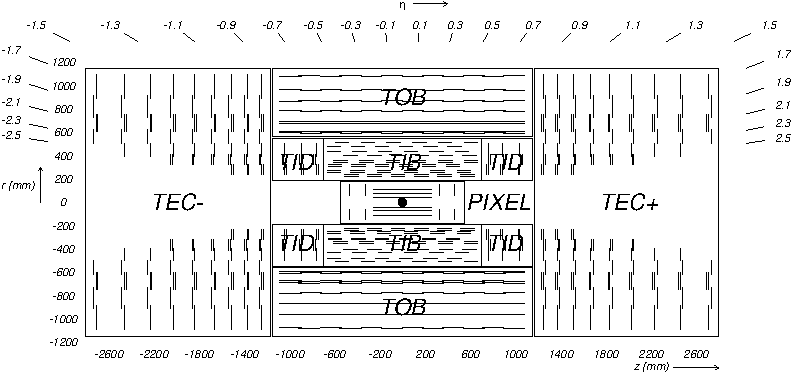
\includegraphics[width=0.55\textwidth]{CMS/tracker}
        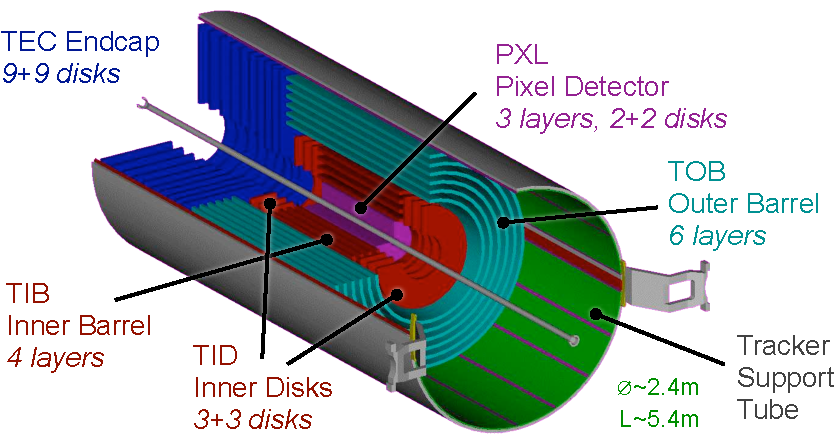
\includegraphics[width=0.44\textwidth]{CMS/tracker3D}
        \caption{Layout of the tracker system.
        On the left, red lines represent pixels, blue lines represent double-sided
        strips modules and black lines represent single-sided strips modules. On the
        right, a 3D representation of the tracking system is presented. The pixel
        is represented in magenta and the different parts of the strips system are
        represented in red, teal and blue.}
        \label{fig:CMS/tracker}
    \end{figure}

    The tracker system is made of several sensors arranged in layers, in turn arranged
    in modules, as represented in \reffig{fig:CMS/tracker}. At the center, the pixel module
    uses silicon pixel sensors of $100 \times 150~\mu\text{m}^2$, providing a resolution
    on the position of hits around $10~\mu\text{m}$ in the transverse plane and
    $20~\mu\text{m}$ in $z$. The barrel module is composed of three layers long of 53 cm in the
    region $r < 10$ cm, supplemented by two disk layers placed at $\left|z\right| \approx$
    35 and 45~cm to cover the forward region. In total, the pixel detector contains 66
    million pixels covering about 16~m$^2$.

    The rest of the tracker system is based on silicon microstrips with a pitch (equal
    to the strip width plus the space between strips) ranging
    from $80$ to $205~\mu\text{m}$ and length ranging from $10$ to $25~\text{cm}$.
    The resolution of these sensors on the hit position ranges from $23$ to $52~\mu\text{m}$
    in the transverse plane and from $230$ to $530~\mu\text{m}$ along $z$.
    This strip tracker is divided in two barrel subdetectors, the tracker inner barrel
    (TIB) and outer barrel (TOB), supplemented by two endcap modules, the tracker inner
    disks (TID) and tracker endcaps (TEC). The strips tracker contains 9.6 million strips
    and cover almost 200 m$^2$ of surface. Overall, the system has a length of 5.6~m
    and a radius of 1.1~m and covers up to $\abseta \approx 2.5$.

        \subsubsection{Electromagnetic calorimeter}

    The role of the electromagnetic calorimeter (ECAL) is to measure the energy of incoming electrons
    and photons. The specifications of this subdetector are particularly oriented for
    the search for the Higgs boson in the $h \rightarrow \gamma \gamma$ channel. The resolution on the
    invariant mass of the diphoton system depends directly on the energy and angular
    resolution of the photons. This part of the detector is of course also crucial for
    all processes involving electrons, such as $Z$ and $W$.

    The technology adopted for the ECAL is lead tungstate crystals (PbWO$_4$). Lead
    tungstate is a very dense scintillation material, about 8.3~g/cm$^3$, with a short
    radiation length 0.89~cm, making it an appropriate choice for a compact calorimeter.
    On the other hand, the light output is relatively low, about 4.5 photoelectrons
    per MeV, and thus requires the use of photo-multipliers to improve the signal collection.
    In the barrel, the calorimeter uses crystals with a size of $2.2\times2.2~\text{cm}^2$
    for the front face and 23~cm in length, as represented on \reffig{fig:CMS/ECALcrystal}.
    In terms of $\eta-\phi$, each crystal covers a region of approximately $0.0174
    \times 0.0174$.

    \insertFigure{CMS/ECALcrystal}{0.6}{PbWO$_4$ crystal used in the ECAL with the photo-diode
    glued to the back of the crystal.}

    In the endcaps, to help to discriminate between prompt photons and $\pi^0$ decaying
    to two directionally close photons, two preshower disks are placed in front of the
    ECAL. Their role is to initiate electromagnetic showers and provide a finer granularity
    with silicon strips 0.2~cm wide, to be compared to the $\sim2\times2~\text{cm}^2$ faces
    of the crystals.

    \insertFigure{CMS/ECAL}{0.7}{Layout of the electromagnetic calorimeter. Each of the
    blue segments represent a PbWO$_4$ crystal.}

    The general layout of the ECAL is presented on \reffig{fig:CMS/ECAL}. The ECAL
    barrel (EB) extends to $\abseta = 1.479$, supplemented by the ECAL endcap (EC)
    up to $\abseta = 3.0$. The preshower disks cover the region $\abseta \in [1.653,2.6]$.
    Overall, the system is $7.8~\text{m}$ long and lie within $1.2 < r < 1.8~\text{m}$
    in the barrel.
    The optical properties of the crystal are crucial parameters that depends on the
    temperature and radiations received. To obtain accurate measurements, a cooling
    system ensure that the crystal temperature is stable at $18\pm0.05^o\text{C}$ and the
    transparency is monitored in real time via a laser system.

    The resolution measured using electrons is parametrized using the formula
    \eq{ECALresolution}
    {
        \left( \frac{\sigma_E}{E} \right)^2
        =
        \left( \frac{S}{\sqrt{E}} \right)^2
        \oplus
        \left( \frac{N}{E} \right)^2
        \oplus
        C^2
    }
    with the different parameters
    \eqalign{ECALresolution2}
    {
        S & = 0.028~\text{GeV}^{1/2} \text{, the stochastic contribution,}\nonumber\\
        N & = 0.12~\text{GeV}\text{, the noise contribution,}\\
        C & = 0.003\text{, the constant contribution.}\nonumber
    }
    This corresponds to a relative uncertainties of 12\%, 1.5\% and 0.4\% for particles
    of $1$, $10$ and $100\GeV$ respectively.

        \subsubsection{Hadronic calorimeter}

    The hadronic calorimeter (HCAL) role is to measure the energy of incoming charged
    and neutral hadronic particles, which will be in turn a crucial information to
    reconstruct jets and missing transverse energy.

    The main technology used for the HCAL consists of layers of dense absorbers and
    scintillation tiles. The absorbers are made of steel and brass, with which
    the incoming hadrons interact to develop a shower. As the particles of the shower
    travel through the calorimeter, they encounter scintillator layers in which they
    emit light. The light is gathered by fibers inside the tiles, which is then
    linked to readout electronics.

    \insertFigure{CMS/HCAL}{0.7}{Layout of the hadronic calorimeter.}

    The layout of the HCAL is presented on \reffig{fig:CMS/HCAL}. The HCAL barrel
    (HB) extends to $\abseta \approx 1.4$ while the HCAL endcap (HE) extends up to
    $\abseta \approx 3.0$. The segmentation term of $\eta,\phi$ is about $0.087 \times 0.087$
    in the barrel which is 25 times coarser than ECAL. A last layer of the HCAL called
    the HCAL outer (HO) uses the magnet coil as an absorption layer. HO is exclusively
    made of scintillation tiles and complements the measurement of the HB. Finally, to
    measure hadrons produced in the high-forward region, two calorimeters (HF) are located at
    $\left|z\right| \approx 11.2$~m to cover $\abseta$ up to 5.2. As they receive a high flux of
    particles coming from underlying events, the material for these calorimeters must
    be able to endure the higher level of radiations and use hard quartz fibers instead of
    plastic ones.

    The resolution measured on pions is
    \eq{HCALresolution}
    {
        \left( \frac{\sigma_E}{E} \right)^2
        =
        \left( \frac{S}{\sqrt{E}} \right)^2
        \oplus
        C^2
    }
    with
    \eqalign{HCALresolution2}
    {
        S & = 0.084~\text{GeV}^{1/2} \text{, the stochastic contribution,}\\
        C & = 0.074\text{, the constant contribution.}\nonumber
    }
    This corresponds to a relative uncertainties of 11\%, 7.9\% and 7.4\% for particles
    of $1$, $10$ and $100\GeV$ respectively.

        \subsubsection{Muon system}

    The muon system is composed of several subsystems placed in the return yoke of
    the superconducting magnet as represented in \reffig{fig:CMS/muon}. It aims to
    measure accurately the trajectory of muons.

    \insertFigure{CMS/muon}{0.7}{Layout of the muon system.}

    Three different gas-based technologies are used, whose choice was driven by the
    large surface to be covered and the radiation environments:
    \begin{itemize}
        \item \textbf{Drift tubes} (DT) - This technology uses stretched wires within
            a gas volume. Charged particles travelling through the gas ionize atoms,
            leaving a cloud of electron along the track. These electrons then drift
            in the tube and are collected by the positively-charged wires. By knowing
            the point where the electrons were collected along the wire, and the
            drift time, it is possible to infer the position of the hit in the drift tube.
        \item \textbf{Cathode strip chambers} (CSC) - Cathode strip chambers are
            made of array of anode wires crossing cathode strips within a gas volume.
            A charged particle travelling through the gas ionizes atoms and provokes an
            avalanche of electrons. The electrons and ions move to the anode and
            cathode respectively, producing a signal in both of them which leads to
            a bidimensional information.
        \item \textbf{Resistive plate chambers} (RPC) - Resistive plate chambers are
            made of two plates of high-resistivity plastic acting as cathode and anode
            separated by a gas volume. After ionization of the gas causing an
            electron avalanche, the charges travel through the plastic plates to be
            collected by strips situated behind them.
    \end{itemize}

    The DT technology is used in the barrel, up to $\left|z\right| \approx 6.5~\text{m}$, covering
    pseudo-rapidities up to $\abseta = 1.2$, while the CSC technology is used for the endcaps,
    where the background rate is large and the magnetic field is also large and non-uniform,
    between $\left|z\right| \approx 6~\text{m}$ and $\left|z\right| \approx 10.5~\text{m}$
    covering up to $\abseta = 2.4$. The RPC complements the previous technologies for
    $\abseta$ up to 1.6, providing a coarser position resolution but a faster response
    and better time resolution.

    When combining the information of the muon system with the tracker, one can
    obtain a relative resolution on the $p_T$ typically of $1\%$, and a relative
    resolution on $\eta$ and $\phi$ typically of the order of $10^{-5}$ and $10^{-4}$
    respectively.

    \subsection{Trigger system}

    The CMS detector must sustain a rhythm of one bunch crossing each 50 or 25 ns, depending
    on the condition of the LHC machine. The raw output of the detector is therefore
    about $20\sim40$~MHz. It is unrealistic to consider storing and reconstructing all these events
    considering the speed of the link to the network, the memory and the computing power
    it would require. Therefore, a selection must be applied online to reduce the rate
    to a more realistic one, set to about $400~$Hz.

    The system in charge of this task is called the trigger \cite{CMStrigger}. The reduction of the rate
    is done by performing a minimalist identification of the features in the event (such
    as significant calorimeter deposits, or hits in the muon system), followed by a more
    complete reconstruction of the objects, and applying thresholds at each steps to
    decide quickly whether the event might be or not relevant for physics analysis.
    The design of these thresholds must be done carefully to have an adequate balance
    between keeping the rate low, while maintaining a high efficiency for the relevant
    physics processes. In this sense, it is also important to optimize the execution
    time of the software as well as obtaining a good accuracy of the minimalist
    reconstruction to efficiently use the available resources.

    The trigger system of CMS is composed of two levels. The level 1 (L1) trigger first
    reduces the rate from $40~$MHz to $100~$kHz, followed by the high-level trigger (HLT)
    which further reduces the rate to $400~$Hz.

    \insertFigure{CMS/triggerL1}{0.8}{Architecture of the L1 trigger.}

    The L1 trigger takes information from the calorimeters and muon system as input
    and is itself composed of different stages as
    represented on \reffig{fig:CMS/triggerL1}. The first stages, the trigger primitives,
    are from the front-end electronics, at the closest of the subsystems.
    These primitives are merged into the regional calorimeter and muon triggers,
    identifying significant energy deposits or muon hits in independent regions of the
    detector. These regional triggers produce a list of muons, $e/\gamma$ candidates
    and local energy deposits. This information is fed to the global calorimeter and
    muon triggers which combine it and remove redundant information. The final global trigger applies
    the trigger menu, that is the set of requirements applied on the final list of
    objects. L1 triggers range from simple single objects with a $\pT$ threshold,
    for instance single electron triggers, to
    selection requiring the coincidence of several objects with topological conditions
    on them, such as a muon plus several jets. Generally speaking, the total rate of
    a given signature decreases as the variety and number of objects it contains increase.
    It is therefore possible to put lower threshold on complex selections compared to
    simpler ones: for instance, the $\pT$ thresholds for an $e+\mu$ trigger can typically
    be set to lower values compared to a dimuon trigger for the same rate, itself having
    lower thresholds than a single muon trigger.

    If the events pass any of the selection in the L1 menu, it is handled to the HLT.
    The HLT selection consists of a much larger list of paths compared to the L1.
    It is done on a computer farm able to perform a full reconstruction
    of the objects present in the event, including the information from the tracker.
    This reconstruction aims to be as close and accurate as possible as compared to the
    offline reconstruction described in the next sections.
    However, some particular techniques may not be used if they are too expensive in
    terms of CPU resources. Furthermore, the processing steps are carefully designed in order to
    optimize the processing time, especially by working as much as possible with steps
    of increasing complexity and possibly filtering some of the events in the middle
    of the procedure. For instance, selection steps involving only calorimeters and
    muon detectors are performed before any tracking reconstruction is required, as this
    last step is CPU intensive. Once an event is selected, it is stored to be used in
    offline physics analysis.

    \subsection{Object and event reconstruction}

    After recording an event, the outputs of each subdetector
    are analyzed to identify the nature and properties of particles produced in the
    event. Ultimately, one want to reduce step by step the complexity of an event to
    something physically understandable. Here, we briefly present some of the
    cornerstones of the CMS reconstruction. First, the tracking and vertexing steps
    correspond to the identification of tracks left by charged particles in the tracker
    and the collision vertices. This step is a crucial point for the second part, the
    particle flow algorithm, which combines measurements from the tracker, muon systems
    and calorimeters to produce a collection of reconstructed particles. In a third step,
    jets of particles can be constructed using clustering algorithms to reach the original
    parton momentum and direction, and a general momentum imbalance can be computed
    to sign the production of particles that escaped detection.

        \subsubsection{Tracking and vertexing \label{sec:trackingAndVertexing}}

    The challenge that the tracking step must address is to use the hits in the
    tracker layers to find and reconstruct the tracks of the $\orderOf{10^3}$ charged
    particles produced in each bunch crossing. If badly designed, this step can lead
    to increased computing time because of the large possible combination of hits one
    has to try, or a high fake rate. The tracking algorithm must therefore be efficient
    in time, but also have a good reconstruction efficiency and a low fake rate.

    The CMS tracking algorithm \cite{CMStracking} starts by constructing seeds from pairs or triplets of hits
    in the pixel detector, compatible with the beamspot. Then, assuming that these
    hits are coming from a charged particle, the trajectory is extrapolated to the
    next layers. If a hit is found compatible with the extrapolation, it is used to
    update the track parameters estimation. Finally, once some criteria are reached,
    such as no more hits to be expected in the detector, the algorithm stops and a
    final fit is performed to determine the track parameters. Then, an iterative procedure removes the
    hits associated to reconstructed tracks, and repeats the track reconstruction
    from new seeds with looser criteria.
    The track reconstruction efficiency for muons is found to be very good as it is
    higher than 99\% up to $\abseta \sim 2.4$, whereas for pions the efficiency varies
    between 85 and 95\% depending on $\pT$ and $\eta$. \reffig{fig:trackingAndVertexingPerf}
    shows on the left the relative resolution on the $\pT$ of isolated muons, which
    is typically about 1-2\% in the barrel and for $10 < \pT < 100\GeV$.

    \insertTwoFigures{trackingAndVertexingPerf}
                     {CMS/trackingPtResolution}
                     {CMS/vertexingZResolution}
                     {0.49}
                     {On the left: relative resolution in $\pT$, as function of the $\pT$, for the
                     tracking of isolated muons in the different $\abseta$ intervals corresponding
                     to the barrel,
                     the transition region and the endcap ; the solid and open dots correspond respectively
                     to a half-width of 68\% and 90\%. On the right: absolute resolution on the
                     primary position as function of the number of tracks of the vertex,
                     for two kinds of events \cite{CMStracking}.}

    Reconstructed tracks are used to identify collision vertices, called primary
    vertices\footnote{As opposed to secondary vertices which occur for example in the
    hadronization of $b$ quarks.}. Only good quality tracks are used in the process, based on their
    compatibility with the beam spot, the number of hits and their fit quality. A
    metric is defined from the closest approach of the track to the $z$-axis and
    the associated uncertainty coming from the track measurement. Then, a deterministic
    annealing algorithm \cite{DAclustering} is used to cluster the tracks into vertices. Compared to the
    traditional jet algorithm that will be discussed later, this algorithm is a divisive
    clustering algorithm: at first, all tracks are put in a single group, which is then
    iteratively divided in smaller groups until a given condition is met. Once it is
    done, the tracks of each group are used to fit the position of the initial vertex.
    The resolution on the vertex position in $(x,y,z)$ depends on the number of tracks
    associated to the vertex, being about 0.1~mm when the vertex has only 5 tracks, and
    down to 10-20~$\mu$m when it has more than 40 tracks as shown on \reffig{fig:trackingAndVertexingPerf} for $z$.
    \reffig{fig:CMS/vertexing} illustrates the vertexing capabilities in an event with
    78 vertices reconstructed. Finally, the primary collision vertex is defined as the
    vertex with highest $\sum_\text{tracks} ({\pT}^2)$.

    \insertFigure{CMS/vertexing}{0.8}{Zoom on the beamspot region of an impressing event
    containing 78 reconstructed vertices.}

        \subsubsection{Particle flow algorithm}

    The role of the particle flow algorithm \cite{particleFlow} is to efficiently combine the output of each
    subdetector to reconstruct each kind of particle according to its nature. Thanks
    to a development before the data taking, it has quickly become the most common
    method of reconstruction used for physics analysis such as cross-section measurements
    and searches for new physics. Particle flow is especially relevant in the context
    of jet clustering that will be presented in the next section: the tracker provides
    key information such as the direction at the vertex for low $\pT$ charged particles
    whereas the calorimeters are better suited in the high $\pT$ regime and for neutral
    particles.

    To combine the outputs of the subdetectors, links are created between elements
    to create blocks. Given the granularity of the detector, blocks are typically made
    of one, two or three elements. For instance, reconstructed charged-particle tracks
    are used to extrapolate the trajectory of the particle to the ECAL and HCAL layers.
    If energy deposits are found nearby the predicted hit using the $\Delta R$
    metric, the track is linked to the energy deposits. Similarly, tracks in the
    tracker can be linked to tracks in the muon system under the condition that the
    global fit of the two tracks is good enough, using a $\chi^2$ as metric.

    The reconstruction of electron is more challenging as they are significantly
    affected by Bremsstrahlung while traveling through the layers of the tracker
    and may radiate photons. In an attempt to collect and link those photons to the
    charged-particle track, tangents to a track at each layer are extrapolated to the
    ECAL and compatible energy deposits are linked to the track.

    After this link step, the identification step is performed from the least ambiguous
    object to the most ambiguous object. Each time an object is identified, it is
    removed from the algorithm before starting the next identification step.

    The least ambiguous objects, the muons, are identified from blocks made of compatible
    tracks in the tracker and the muon system. Then, electrons are considered from
    block made of tracks and energy deposits in the ECAL. The exact treatment for
    electrons is more careful than for other tracks, as the fit of the track must take
    into account the successive loss of energy due to Bremsstrahlung in the tracker
    layers. Therefore, the tracks are refitted using a Gaussian-Sum filter (GSF)
    \cite{GSFelectrons} which takes this phenomena into account. The final identification
    involve criteria on the tracking, calorimetric and compatibility variables.

    After the charged leptons identification, criteria are applied on the remaining
    tracks and those are considered to be charged hadron candidates. Their energy
    and momentum are computed either from the track alone assuming a charged pion
    hypothesis, or by combining the track and calorimeter information which is relevant
    in particular at high $\pT$ or large $\eta$ where the tracker resolution is
    degraded. Finally, after subtracting the energy deposits from charged particles
    in the ECAL and HCAL, the remaining significant energy deposits give rise to photon
    candidates and neutral hadron candidates.

    \subsubsection{Jet reconstruction \label{sec:jetReconstruction}}

    The concept of jets refers to collimated bunches of stable hadrons coming from partons
    (quarks or gluons) after they fragment and hadronize. Reconstructing jets can
    therefore yield information regarding quarks or gluons produced in the event.
    Jets are defined from the choice of algorithm to reconstruct them as well as the
    parameters used. It can not be stressed enough that there is no direct equivalence
    between a jet and a parton: the interpretation of a jet is fundamentally ambiguous
    as one parton shower can overlap with another. Moreover, a jet can be contaminated by other
    hadronic activity in the event, such as pile-up, which can degrade the energy
    and angular resolution. Jet physics is therefore a very rich topic and a field
    in itself, which goes from theoretical QCD to models of hadronization, jet
    reconstruction, calibration and study of the jet substructure.

    Two main categories of algorithms exist to build jets: cone-based algorithm and
    incremental clustering algorithm. CMS mainly uses two incremental clustering
    algorithms. The starting point is the definition of the metric between objects in the
    event, which may be for instance the energy deposits in the calorimeters or the
    particle flow collection. The main algorithm is called anti-$k_T$ \cite{antiKt} and uses a metric
    defined by
    \eq{jetClusteringMetric}
    {
        d_{ij} \definedAs \text{min}(p^{2p}_{T,i},p^{2p}_{T,j}) \frac{\Delta R^2_{ij}}{r^2}
    }
    where $p = -1$ for anti-$k_T$, $p_{T,i}$ (resp. $p_{T,j}$) is the value of the transverse momentum of
    the $i$-ish (resp. $j$-ish) object, and $r$ is a size parameter, analogous to the size of a cone and
    typically equal to 0.5 for CMS during Run I. Objects with the smallest $d_{ij}$ are
    merged together into a protojet. The procedure is repeated until all the objects have
    $d_{ij}$ larger than $r$. In the
    simple case with one high-$\pT$ object surrounded by several softer objects, this
    leading object will aggregate all the softer ones and the result is a cone-like jet. When
    there are two or more high-$\pT$ objects in the event, they either get merged into
    a single jet ($\Delta R < r$) with a cone-like shape around their barycenter, or
    lead to two separated jets ($\Delta R > r$) where the dominant object will first
    aggregate the softer objects. An example of jet reconstructed with this algorithm
    is shown in \reffig{fig:CMS/jetExample}.

    The second algorithm, called Cambridge/Aachen algorithm \cite{CA}, uses the metric from
    \refequation{eq:jetClusteringMetric} but with $p = 0$, i.e. not relying on the $\pT$ of
    the objects but only on their angular proximity. The shape of the jets obtained with
    this algorithm are less likely to be cone-like. Nevertheless, it has been found to
    yield better results for substructure-oriented studies of jets.

    \insertFigure{CMS/jetExample}{0.6}{Representation of a $115\GeV$ jet reconstructed in CMS
    with the anti-$k_t$ algorithm, showing the reconstructed tracks left by charged
    particles in plain blue lines, and the trajectory of neutral particles in dotted
    lines \cite{QuantumDiariesJets}. The electromagnetic and hadronic deposits in calorimeters are represented
    in lego plots in yellowish and teal respectively. One should note how the curved
    trajectory of some charged particles make it so that they actually leave the
    pseudo-cone when flying out of the vertex.}

    Experimentally, jets are typically made of 10-20 particles, and about 65\% of the
    energy is carried by charged hadrons, 25\% by photons and 10\% by neutral hadrons
    at $100\GeV$ \cite{JetPerf}.
    \reffig{fig:jetEfficiencies} presents a comparison of the performances obtained
    for particle-flow jets and calorimeter-based jets. For a given initial parton, the
    probability to successfully reconstruct a jet in $\Delta R < 0.1$ reaches 90\% for
    a parton of $30\GeV$ for particle-flow jets compared to $80\GeV$ for
    calorimeter-based jets. In terms of $\pT$ resolution, the reconstructed $\pT$ is
    roughly within $90\% \pm 15\%$ of the generated $\pT$ for the particle-flow jets
    when $40 < \pT^\text{gen.} < 60\GeV$, whereas it is within $50\% \pm 15\%$ for
    calorimeter-based jets \cite{particleFlow}. This bias in the reconstructed transverse momentum, called
    jet energy scale, is typically due to thresholds and inefficiencies in the calorimeters
    and can be measured and corrected after the jet reconstruction. This correction is
    typically parametrized as function of $\pT$ and $\eta$.

    \insertTwoFigures{jetEfficiencies}
    {CMS/jetMatchingEfficiency}
    {CMS/jetResolution}{0.49}
    {Comparison of some performances for the jet reconstruction using particle flow as
    input compared to a calorimeter-based approach \cite{particleFlow}. On the left, jet matching efficiency
    as function of the generated $\pT$ in the central region $\abseta < 1.5$, effectively
    corresponding to the probability of successfully reconstructing a jet within
    $\Delta R < 0.1$ of the generated parton. On the right, relative difference between
    the reconstructed and generated $\pT$ for initial partons with $40 < \pT^\text{gen.} < 60\GeV$.
    }

        \subsubsection{Missing transverse energy}

    So far it has been shown how to reconstruct charged leptons and photons and get
    information regarding quarks and gluons produced in the event. The remaining
    type of stable particles one expects from the Standard Model is neutrinos, which
    have very low rate of interaction with matter and therefore escape detection. Some
    theories beyond the Standard Model also include stable particles escaping detection
    such as neutralinos in R-parity conserving SUSY.

    It is possible to infer information about the production
    of such particles via the energy-momentum conservation in the transverse plane\footnote{The
    longitudinal plane can however not be used, since the two incoming partons carry
    different, unknown momenta.}. A significant imbalance may reveal the momentum carried by
    the sum of invisible particles. We define the missing transverse energy as the
    sum of transverse momenta:
    \eq{ETmissDefinition}
    {
        \vec{\MET} \definedAs - \sum_{\text{objects}} \vec{\pT}.
    }
    In this formula, one must define what are the objects to consider and this choice
    leads to several possible reconstructions, such as calorimeter-based, track-based
    or PF-based $\MET$. Several effects may lead to artificial $\MET$, in addition to the
    genuine $\MET$ from invisible particles, which can be classified in two categories:
    intrinsic condition and resolution of the detector, for instance the jet energy
    resolution ; and misreconstruction of the events or mismeasurement in the
    operation of the detector, for instance in the operating of the laser correction
    of the ECAL. One of the challenges of $\MET$ reconstruction is therefore to identify
    and understand the different sources of unphysical missing energy as well as biases and
    smearing, and either correct them to improve the resolution or veto the corresponding
    events.
    \reffig{fig:METspectrum}, on the left, shows how sources of unphysical $\MET$
    lead to an unexpected large tail in the reconstructed distribution for the data \cite{METperf}.
    After identifying several causes and filtering out events likely to have unphysical
    $\MET$, the agreement between data and simulation is restored.

    \begin{figure}[h!]
        \centering
        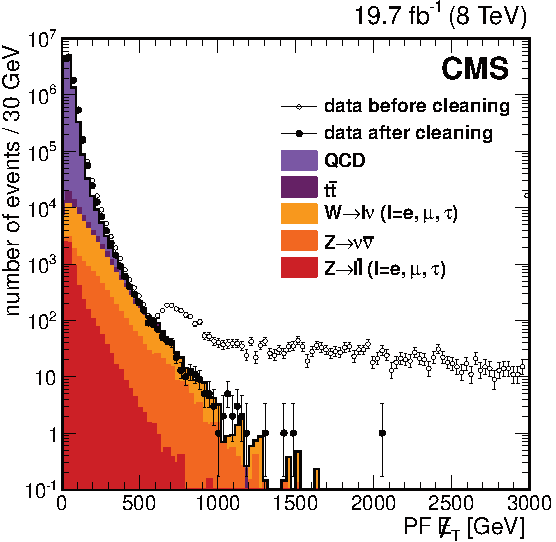
\includegraphics[width=0.53\textwidth]{CMS/MET/cleaning}
        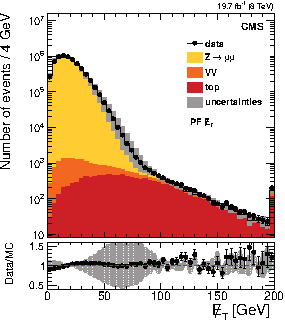
\includegraphics[width=0.45\textwidth]{CMS/MET/spectrumInZmumu}
        \caption{On the left, comparison of data with simulation of the
        particle-flow based $\MET$ distribution, before and after cleaning of the events
        likely to contain unphysical $\MET$. On the right, distribution of $\MET$ in
        a $Z \rightarrow \mu\mu$ enriched sample \cite{METperf}. }
        \label{fig:METspectrum}
    \end{figure}

    Events with no genuine $\MET$ provide a mean to study the resolution.
    $Z \rightarrow \mu\mu$ events fit well this purpose as muons are well-identified objects
    with a good resolution and a constraint can be put on the invariant mass of the
    dimuon system to obtain a sample with good purity. \reffig{fig:METspectrum},
    on the right, shows the distribution of the reconstructed particle-flow based
    $\MET$ in such events. The maximum of the distribution is around $10-20\GeV$ and
    drops by three orders of magnitude up to $70-80\GeV$.

    The resolution can be studied as function of the recoil of the $Z \rightarrow \mu\mu$
    system due to initial state radiations, and also as function of the pile-up in the
    event, as presented on \reffig{fig:METresolution}. We introduce $\vec{q_T}$,
    the measurement of the energy-momentum of the $Z$ from the dimuon system, i.e.
    $\vec{q_T} \definedAs (\vec{p}_{T,\mu_1} + \vec{p}_{T,\mu_2})$. We use all the other
    reconstructed particles in the event to define $\vec{u}_T \definedAs \sum_{\text{non-}\mu} \vec{p}_{T,i}$,
    which in the ideal case should correspond to the energy momentum of the sum of the
    ISR and perfectly balance with $\vec{q}_T$. Finally, we introduce $u_{||}$ as the
    projection of $\vec{u}_T$ on the axis defined by $\hat{q}_T \definedAs \vec{q}_T
    / q_T$, i.e. $u_{||} \definedAs \vec{u}_T . \hat{q}_T$.

    \begin{figure}[h!]
        \centering
        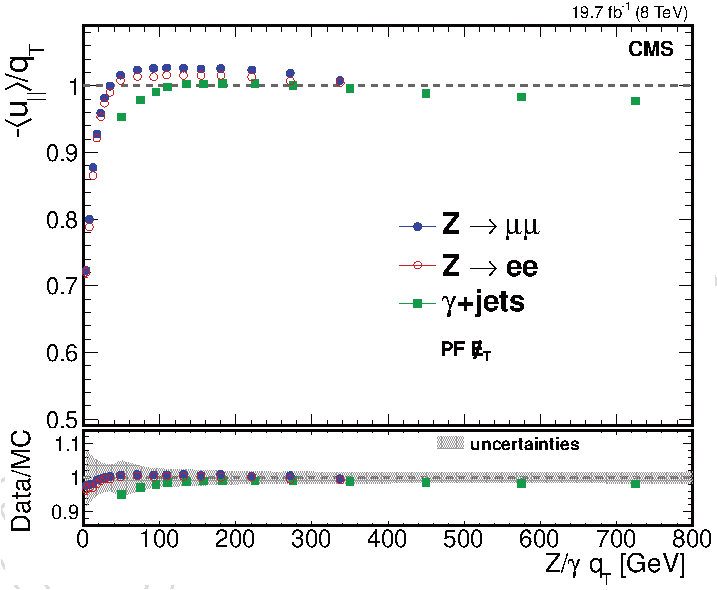
\includegraphics[width=0.58\textwidth]{CMS/MET/resolutionVsQt}
        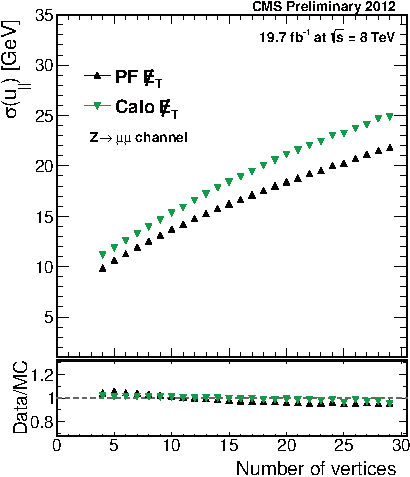
\includegraphics[width=0.41\textwidth]{CMS/MET/resolutionVsPU}
        \caption{On the left, measurement of the ratio $-u_{||}/q_T$ as function of $q_T$
        in $Z\rightarrow\mu\mu$, $Z\rightarrow e e$ and $\gamma$+jets events using
        the particle-flow based $\MET$. On the right, measurement of the resolution of
        $u_{||}$ as function of the number of reconstructed primary vertices, for
        $Z\rightarrow\mu\mu$ events \cite{METperf}.}
        \label{fig:METresolution}
    \end{figure}

    At low $q_T$, the ISR is essentially too soft to be measured accurately, and
    therefore $- u_{||}$ is quite different from $\vec{q}_T$. At $q_T \sim 40\GeV$,
    however, the measurement of the ISR gets better and $u_{||}$ is within $\sim 3\%$
    of $q_T$. In addition, the resolution of $\vec{u}_{||}$ strongly depends on the
    pile-up activity since more hadronic activity tends to increase jet energy
    mismeasurement.

    \section{Collisions and detector simulations \label{sec:simu}}

    After registering the events from the detector, and reconstructing the particles
    produced, one needs a mean to compare the experiment with theories. Given
    the complexity of a single bunch crossing, including the hard scattering,
    underlying events and pile-up, and the complexity of the detector, the distribution
    of observables can not in the general case be predicted analytically. One must
    instead rely on Monte-Carlo generations and an accurate detector simulation.
    Such a tool can also help in designing the detector in the first place, for
    instance by studying the performances on a given process, all the way
    from the hard scattering to the objects after reconstruction.

    The full chain of simulation can be implemented as follow. First, the model
    is implemented and the Feynman rules associated to the Lagrangian are computed.
    Then, for a given process, a Monte-Carlo generator computes all possible
    Feynman diagrams up to a given order, and randomly generates hard-scatterings.
    To these hard-scatterings are added the underlying event as well as initial and
    final state radiations, and the quarks are hadronized. Finally the particles
    are propagated to the detector and its response is simulated, after which
    the reconstruction process is essentially the same as for data.

    \subsection{Monte-Carlo generation of the hard scattering}

    To get a better idea on how Monte-Carlo event generation of the hard scattering
    is performed, it is useful to take a simple example such as the diagram
    $u\bar{u} \rightarrow Z \rightarrow d\bar{d}$ at tree level \cite{MCGenLesHouches}. The corresponding
    infinitesimal cross section is
    \eq{crossSectionEventGeneration}
    {
        d \sigma(u\bar{u} \rightarrow Z \rightarrow d\bar{d})
        =
        \frac{1}{2\hat{s}}
        \left|
            \mathcal{M}(u\bar{u} \rightarrow Z \rightarrow d\bar{d})
        \right|^2
        \frac{d\cos(\theta)\, d\phi}{32\pi^2}
    }
    where $(\theta,\phi)$ are the angles of the $Z$ decay, $\mathcal{M}$
    is the matrix element and $\hat{s}$ is the center of mass energy. The matrix
    element is, for a given diagram, a number computable from the Feynman rules.
    To generate events according to this simple process, one may draw random
    values of $\cos(\theta)$ and $\phi$, uniformly distributed in $[-1, 1]$ and
    $[0,2\pi]$ respectively. From the masses constraints and the directions of the
    decay products, it is then possible to compute the quadri-momentum of the products.

    The value of $d\sigma$ is directly related to the probability for this event
    to occur and is different for each value of $\cos(\theta)$ and $\phi$. To obtain
    a set of events with distributions of $\cos(\theta)$ and $\phi$ corresponding to
    what is to be observed in Nature, it is possible to unweight these events using
    for instance a hit-and-miss technique.

    With these simple steps, we presented the basic procedure to build a Monte-Carlo
    event generator. However in real life, and in particular in the case of the
    LHC, the initial state is made of protons. Therefore, in order to obtain a
    description of actual collisions, one must consider instead the process
    $pp \rightarrow Z \rightarrow d\bar{d}$ and integrate over the parton distribution
    function.

    Furthermore, a complete description of such a process must also include
    diagrams with additional partons produced in the event, coming for instance
    from initial or final state radiation, e.g. $pp \rightarrow Z \rightarrow
    d\bar{d}$, $d\rightarrow dg$, or from other diagrams. This level can be called
    LO+jets. Generating diagrams with additional partons in the final state however
    induces an exponentially growing number of diagrams to consider, and one must
    find adequate ways to implement this from a purely software point of view.

    Finally, this brief description focused on tree-level diagrams, but a more accurate
    description of the process can be obtained if one is able to take into account higher order
    diagrams (NLO, NNLO, ...). Generally speaking, NLO is more difficult to
    automatize and, even though softwares are now able to handle NLO generation, it is
    currently still an active field of development.

    \subsection{Hadronization}

    Partons are affected by the strong interaction and cannot exist in free state,
    as discussed in \refsection{sec:strongInteraction}. If partons move away from
    each other with a sufficient energy, this energy will be used to create new colored
    particles and bind into hadrons forming a jet of particles collimated in the
    direction of the initial partons. This process is referred to as hadronization,
    and is a crucial point of event generation as it determines the structure
    of generated jets.

    The number of problematics related to hadronization makes it a quite rich and
    active topic. The interface between the generation of the hard scattering
    and the parton shower is not trivial as no technique rigorously factorizes
    these two problematics. For instance, a gluon emission during
    the parton showering (so-called soft emission) may correspond to an additional
    parton during the generation of the hard process (so-called hard emission),
    ultimately causing double counting and biasing the event set. To solve this
    problem, a factorization prescription, called a matching scheme, must be defined
    to remove this double counting.

    There are different techniques to simulate hadronization \cite{MCGenPDG}. In particular, the
    technique used in the software \textsc{Pythia} is based on the Lund string
    model. In this model, two partons moving away from each other are linked
    via a gluonic string being stretched, its potential energy growing at
    the expense of its kinetic energy. When its potential energy becomes of the
    order of the mass of two quarks, this string is likely to break and pull
    out a pair of quarks out of vacuum. This process goes on until
    hadrons are formed, which may in turn decay according to known branching
    fractions.

    So far, however, hadronization models contain free parameters which are not known,
    essentially due to our lack of understanding at this point of non-perturbative
    QCD. Therefore, the free parameters in these models must be tuned according to
    experiments.

    \subsection{Detector simulation}

    Now knowing the final state after hadronization and decay of the hadrons, we
    want to put the events in the context of a bunch crossing at the LHC. In
    particular, we need to take into account the pile-up. To do so, a number of
    pile-up collisions is drawn according to a distribution similar to the
    one expected in the data. Pile-up collisions are added to the event from a
    set of pre-generated and hadronized events.

    Then, we want to simulate the response of the entire CMS subdetectors. To do
    this, a detailed description of the detector is implemented in the software
    \textsc{Geant4} \cite{Geant4}. Its description can be tuned to study, for instance,
    misalignment condition. The interaction between particles emerging from
    the bunch crossing and the detector material is simulated using physical
    models of radiation-matter interaction, eventually generating a signal in
    the readout electronics. The trigger is simulated as well, though only to know
    which bits are fired rather than filtering out events at this stage. The
    simulation takes up to a few seconds per event.

    Mainly for time constraints, it is in some cases good enough to perform a
    fast simulation of the detector \cite{Fastsim}. In this simulation, the radiation-matter
    interaction is parametrized and leads
    directly to the hits in the tracker and muon systems, and to the showers
    in the calorimeter towers. Hence, the same low-level information as for the
    full simulation is obtained, i.e. hits and energy deposits as measured by
    the electronics, and the same reconstruction algorithms can be applied.
    Overall, avoiding the CPU-intensive simulation of the radiation-matter interaction
    in \textsc{Geant4} allows to speed up the simulation by a factor 100-400
    depending whether pile-up is included or not.

%==============================================================

\setcounter{mtc}{4}
\chapterwithnum{$b$-tagging techniques and validation in CMS}
\hspace*{0.39\textwidth}
\begin{minipage}{0.60\textwidth}
\emph{« I'm going to need a SWAT team ready to mobilize, street level maps covering all
Florida, a pot of coffee, twelve jammy dodgers and a fez..! »}
\hspace*{0.4\textwidth} The Eleventh Doctor
\end{minipage}
\minitoc
\newpage

%==============================================================

    $b$ quarks are found in the final state of a large variety of Standard Model
    involving top quarks, $Z$ or Higgs bosons, as well as in many BSM processes.
    The hadronization of $b$ quarks produces $B$ hadrons, i.e. hadrons with a structure
    involving a $b$ quark. Thanks to the remarkable properties of $B$ hadrons compared to
    other hadrons,
    it is possible to identify jets originating from the hadronization of $b$ quarks.
    Such identification is done using $b$-tagging algorithms, and represents an important tool used
    by a large fraction of analyses in the CMS collaboration.

    In \refsection{sec:bTagAlgorithms}, we discuss the $B$ hadrons and $b$ jet properties,
    which are the starting point to construct discriminating observables between $b$ jets
    and jets from other flavors. Then, we present how these variables are used to build
    the $b$-tagging algorithms. In \refsection{sec:bTagValidation}, we shall discuss
    the $b$-tagging validation activity within the CMS collaboration, in particular
    focusing on some major validations to prepare the Run II of the LHC.

    \section{Topology of $b$ jets and tagging algorithms \label{sec:bTagAlgorithms}}

    \subsection{Properties of $B$ hadrons and topology of $b$ jets}

    The $B$ hadrons, produced by the hadronization of $b$ quarks, are bound states composed
    of a $b$ quark and one or two other quarks. The study of their decays is
    a field in its own, and of particular importance as such decays are related to the
    CKM matrix and CP violation. $B$ hadrons have particular properties compared to other hadrons
    found in light jets, i.e. arising from the hadronization of $u$, $d$, $s$ quarks or
    gluons, making it possible to identify $b$ jets. It must be noted that $C$ hadrons,
    which are bound states involving a $c$ quark, also share to a lesser extend some of these
    properties, which in turn makes $c$ jets naturally more difficult to distinguish
    from $b$ jets. The properties can be listed as follow:
    \begin{itemize}
        \item \textbf{Large mass} - $B$ hadrons have masses ranging from $5$ to $10\GeV$, as
              they contain a $b$ quark which has a mass around $4.5\GeV$. Such a mass is
              much larger than those of hadrons found in light jets, which have a mass
              typically less than $0.1\GeV$.
        \item \textbf{Long life time and decay length} - $B$ hadrons decay via the weak
              interaction, with a strength proportional to the CKM matrix elements $V_{cb}$ and $V_{ub}$
              which are of the order of $10^{-2}$ and $10^{-3}$ respectively. Because of
              the smallness of these parameters, the life time of $B$ hadrons is about
              $10^{-12}~\text{s}$, corresponding to a decay length of a few tenth of millimeters
              ($10^{-4}~\text{m}$). In comparison, light hadrons have life time of the order
              of $10^{-16}~\text{s}$.
        \item \textbf{High charged multiplicity decays} - $B$ hadron decays typically
              contain 5 charged particles on average, whereas other light hadrons
              usually decay into 1 or 3 charged particles.
        \item \textbf{Leptonic decay} - As the decay of $B$ hadrons involves a virtual $W$ boson,
              they are likely to directly decay leptonically, with a branching ratio of
              11\% per lepton family. This fraction goes up to about 20\% if one
              considers the full decay cascade (which includes $B \rightarrow C +
              \text{hadrons} \rightarrow \ell\nu + \text{hadrons}$).
    \end{itemize}

    In the context of a $b$ jet, several particles including a $B$ hadron emerge from
    the primary vertex where the hard scattering and hadronization occurred. Due to its
    life time, the $B$ hadron decays a few tenth of millimeters away from the primary
    vertex, producing a secondary vertex, as represented on \reffig{fig:bTagging/jetTopology}.
    In the cases where $B$ hadrons decay into a $C$ hadron, a tertiary vertex might
    be produced due to the life time of $C$ hadrons.
    \insertFigure{bTagging/jetTopology}{0.75}
                 {Topology of a jet originating from the hadronization of a $b$ quark: the
                 jet contains a neutral $B$ hadron with a decay length around $0.5~\text{mm}$,
                 producing a secondary vertex with a high multiplicity of charged particles
                 emerging from it.}

    Provided a good enough tracking resolution, such a topology can therefore be identified
    by looking for displaced tracks and the fact that several of them are compatible with
    originating from a common secondary vertex. Other properties may be used, such as the
    distribution of tracks inside the jet, or the presence of a charged lepton. A
    real life example of event containing $b$-tagged jets is shown on \reffig{fig:bTagging/vbfHbb_Candidate},
    taken from a search for $H\rightarrow b\bar{b}$ in the CMS collaboration \cite{HIG-13-011}.

    \insertFigure{bTagging/vbfHbb_Candidate}{0.8}{Illustration of $b$-tagging in an event
    at $\sqrt{s} = 8\TeV$. The display shows the longitudinal view of the surrounding region of the primary vertex
    and the tracks reconstructed, in a $H \rightarrow b\bar{b}$ candidate event produced through
    vector boson fusion (VBF) characterized by the two forward jets. The green tracks are
    prompt tracks while the blue tracks have a high impact parameter significance. On the
    jet at the top of the figure, the red line represents a reconstructed muon. One
    can clearly distinguish the secondary vertices in each of the central jets which have
    therefore a high $b$-tagging discriminant. The invariant mass of the two $b$ candidates
    is found to be close to $125 \GeV$ \cite{HIG-13-011}.}

    \subsection{$b$ jets discriminating quantities and objects}

    \subsubsection{Track selection}

    For a given jet, the tracks considered for $b$-tagging studies must have
    a good quality (normalized $\chi^2_\text{track fit} < 5$ as well as sufficient number of hits in the
    pixel and in the tracker as a whole) and $\pT > 1\GeV$. The tracks must also be within
    $\Delta R < 0.3$ of the jet axis (except for the track counting algorithm which uses $\Delta R < 0.5$).
    As illustrated on \reffig{fig:bTagging/impactParameter}, the points $Q$ on the track
    and $J$ on the jet axis are defined as the points of closest approach between the
    track and jet axis. In a similar way, the point $P$ is defined as the point of closest
    approach on the track with respect to the primary vertex $V$. To reject contamination
    from pile-up and other jets that would be interpreted as displaced tracks, several
    criteria are applied: the distance to jet axis, $JQ$, is required to be lower than
    $700~{\mu\text{m}}$ ; the so-called decay length of the track, $VQ$, is required to
    be lower than $5~\text{cm}$ ; and the track is required to be reasonably compatible
    in the transverse plane with the primary vertex by imposing a closest approach lower
    than 2 mm.

    \insertFigure{bTagging/impactParameter}{0.75}
                 {Representation of two tracks inside a $b$ jet, one coming from a prompt
                 charged hadron and the other from the decay of
                 the $B$ hadron. The prompt track has been slightly displaced from the primary vertex
                 to illustrate resolution effects. One can define along the track the position
                 of closest approach to the primary vertex, $P$, and the closest approach
                 to the jet axis, $Q$. The impact parameter corresponds to the distance $VP$
                 and it is given the sign of the scalar product $\vec{VP} \cdot \vec{j}$ (with
                 $\vec{j}$ being the jet direction).}

    \subsubsection{Impact parameter}

    An important quantity to characterize the displacement of tracks is the impact parameter.
    As represented on \reffig{fig:bTagging/impactParameter}, the impact parameter is defined
    as the distance of closest approach, in the three dimensional space, between the track
    and the vertex, $VP$. Additionally, it is given the sign of the scalar product $\vec{VP}
    \cdot \vec{j}$ where $\vec{j}$ is the jet direction.

    Because of their displacement, tracks from the decay of $B$ hadrons are expected to
    have a large, positive impact parameter. Tracks in light jets are instead expected
    to originate directly from the primary vertex and therefore to have non-zero value
    only due to resolution effects. To integrate the knowledge of the tracking resolution,
    the uncertainty on the impact parameter, $\sigma_\text{IP}$ can be computed for each
    track, and one can define the impact parameter significance, $S_\text{IP} \definedAs
    \text{IP}/\sigma_\text{IP}$.

    \reffig{fig:bTagging/impactParameterDistr} presents the distribution of the
    impact parameter (IP) and impact parameter significance for tracks in $b$ jets, $c$
    jets and light jets. In particular, the distributions drop rapidly for tracks from
    lights jets after $S_\text{IP} = 2$. The distributions for tracks from $b$ jets shows
    a clear large tail in large positive values, but because $b$ jets also contain some
    prompt tracks, a significant fraction ends up with low or negative $S_\text{IP}$
    values.

    \begin{figure}[th!]
        \centering
        \begin{minipage}{\textwidth}
        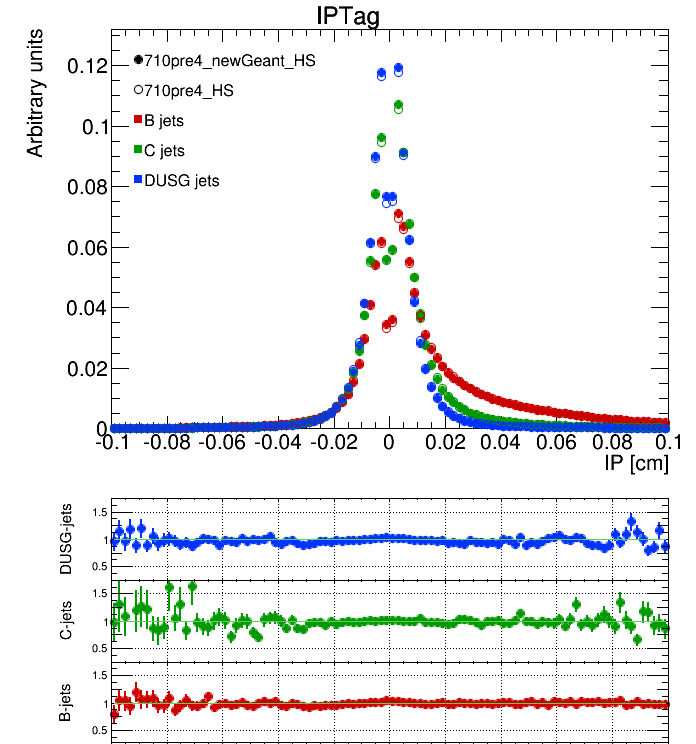
\includegraphics[width=0.49\textwidth]{bTagging/8TeV/TTbar_PU_lowLevelVariables/IPTag_ip_3D_GLOBAL_all}
        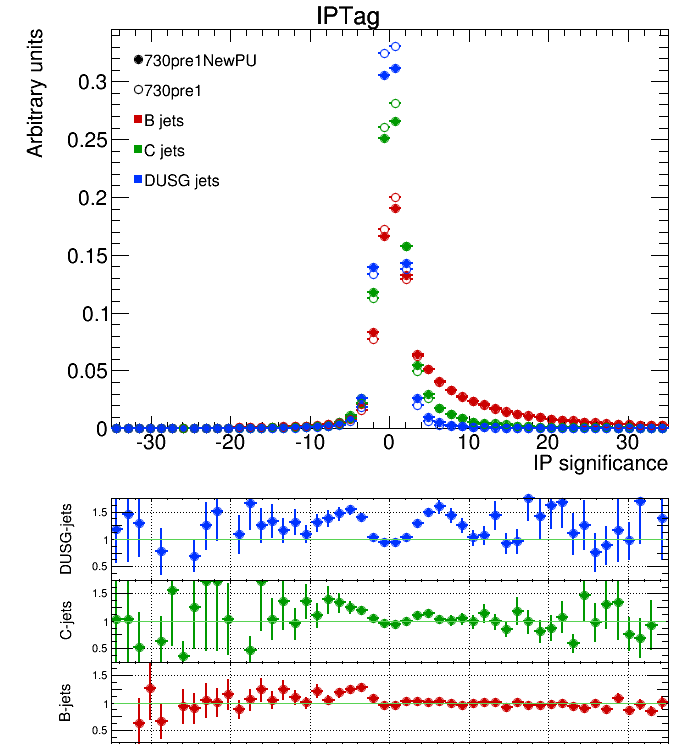
\includegraphics[width=0.49\textwidth]{bTagging/8TeV/TTbar_PU_lowLevelVariables/IPTag_ips_3D_GLOBAL_all}
        \end{minipage}
        \caption{Distribution of the impact parameter (on the left) and impact parameter significance
        (on the right) for tracks
        inside the different jet categories, estimated using the validation framework from a
        $t\bar{t}$ Monte-Carlo sample with Run I conditions, including pile-up.}
        \label{fig:bTagging/impactParameterDistr}
    \end{figure}

    \subsubsection{Secondary vertex}

    As discussed in \refsection{sec:trackingAndVertexing}, the resolution on the primary
    vertex position varies between 100 and 10~$\mu$m. This is less than the typical decay length
    of a $B$ hadron, which makes it possible to attempt to reconstruct the corresponding
    secondary vertex. This can be done using adaptive vertex fitting techniques \cite{AdaptiveVertexFitting},
    similar to the technique used for primary vertices identification, but using parameters
    relevant to this context and in particular to be robust against outliers. Several
    quantities related to secondary vertex candidates can then be computed, such as the
    distance from the primary vertex (or flight distance), the flight direction and the
    vertex mass.

    $B$ hadrons are expected to have a flight distance of a few tenth of millimeters, a
    flight direction within $\Delta R < 0.5$ of the jet direction and a mass of a few$\GeV$.
    To reduce contamination from vertices of long-lived mesons and particle interactions with
    the detector material, secondary vertices with a flight distance higher than $2.5~\text{cm}$
    (i.e. much greater than what is expected for a $B$ hadron) or a mass compatible with
    the mass of $K_0$ or larger than $6.5\GeV$ are rejected.

    \reffig{fig:bTagging/secondaryVertex} presents the distribution of
    the vertex mass and the flight distance significance for the different jet categories,
    showing a clear distinct shape for the distribution of $b$ jets compared to light and
    $c$ jets.

    \begin{figure}[th!]
        \centering
        \begin{minipage}{\textwidth}
        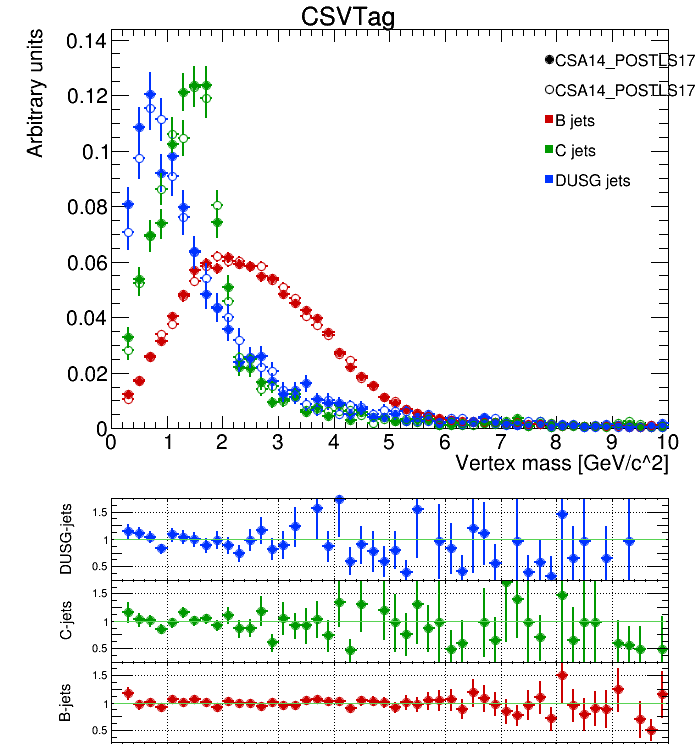
\includegraphics[width=0.49\textwidth]{bTagging/8TeV/TTbar_PU_lowLevelVariables/CSVTag_vertexMass_GLOBAL_all}
        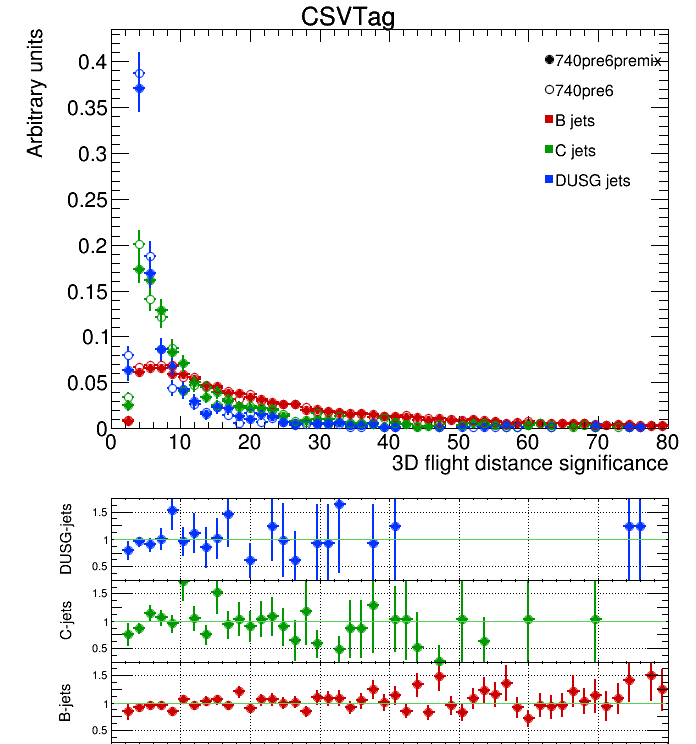
\includegraphics[width=0.49\textwidth]{bTagging/8TeV/TTbar_PU_lowLevelVariables/CSVTag_flightDistance3dSig_GLOBAL_all}
        \end{minipage}
        \caption{Distribution of the secondary vertex mass (on the left) and flight distance significance (on the right)
        for the different jet categories, estimated using the validation framework from a
        $t\bar{t}$ Monte-Carlo sample with Run I conditions, including pile-up.}
        \label{fig:bTagging/secondaryVertex}
    \end{figure}

    \subsubsection{Soft leptons}

    Due to the leptonic decay of $B$ hadrons, a significant fraction of $b$ jets are
    expected to contain a soft charged electron or muon. Despite the intrinsic limitation
    due to the low branching ratio, this specificity remains useful to complement other
    techniques and to enrich a sample of events in $b$ jets as light jets have low probability
    to contain a lepton.

    One useful variable, relating the soft lepton to the jet, is $p_T^\text{rel.}$ defined
    as the projection of the lepton momentum to the plane perpendicular to the jet axis
    $\vec{j}$. In this definition, the jet direction is computed by also including the lepton.
    $p_T^\text{rel.}$ is expected to have larger values in $b$ jets compared to light jets.

    Additionally, the impact parameter significance of the lepton can be considered to
    characterize its displacement with respect to the primary vertex. In that particular
    case, the significance can benefit from the excellent resolution on muon tracking
    provided by the detector.

    \reffig{fig:bTagging/softLepton} presents the distribution of
    the $\Delta R$ between the muon and the jet direction, as well as $p_T^\text{rel.}$ for
    muons inside the different categories of jets, showing the discriminating power that
    they provide.

    \begin{figure}[th!]
        \centering
        \begin{minipage}{\textwidth}
        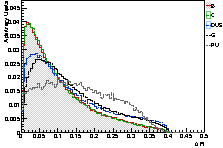
\includegraphics[width=0.49\textwidth]{bTagging/8TeV/muonDeltaR}
        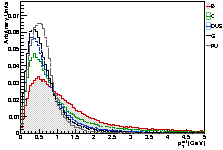
\includegraphics[width=0.49\textwidth]{bTagging/8TeV/muonPtRel}
        \end{minipage}
        \caption{Distribution of $\Delta R(\mu,\text{jet})$ (on the left) and $p_T^\text{rel.}$ (on the right)
        for muons inside different jet categories \cite{SoftLeptonAN}.}
        \label{fig:bTagging/softLepton}
    \end{figure}

    \subsection{$b$-tagging algorithms}

        \subsubsection{Notion of performance}

    Before introducing the algorithms themselves, let's introduce the notion of performance
    of an algorithm. An algorithm associates to each jet a real value, the discriminant,
    whose distribution provides good discrimination between $b$ jets and other jets flavors.
    One then defines an operating point, or threshold, such that jets with discriminant
    larger than the threshold are said $b$-tagged.

    Typically, one wants to study the $b$-tagging efficiency as function of
    the threshold value, that is to say the probability for a given a $b$ jet to be
    successfully $b$-tagged. Similarly, it is relevant to look at the fake rate, i.e. the
    probability that a non-$b$ jet gets incorrectly $b$-tagged. Because the $c$
    jets are harder to differentiate from $b$ jets, the fake rate of these jets is studied
    independently from light jets.

    Performances are usually presented by showing the fake rate as function
    of the $b$ jet efficiency, each point of the curve corresponding to a different threshold
    value. To benchmark the performances and allow easier comparisons
    between algorithms, one can define three operating points, loose, medium and tight,
    such that the fake rate for light jets is respectively 10, 1 and 0.1\%.

    Finally, the performances are likely to depend on the environment in which
    the jets are produced, in particular if there is other hadronic activity coming from
    the hard-scattering, or from pile-up contamination. In this section, the performances
    are obtained using the validation framework, and are computed from a $t\bar{t}$
    Monte-Carlo sample at $\sqrt{s} = 8\TeV$ with pile-up included. Performances at $7\TeV$
    and $8\TeV$ are also discussed in \cite{BTagging7TeV}, \cite{BTagging8TeV}.

        \subsubsection{Track counting algorithm}

    The track counting algorithm is based on the impact parameter of tracks. Tracks are
    sorted according to the value of the impact parameter significance. Because of this
    ranking, the $S_\text{IP}$ of the first track is biased and is likely to be high even
    for light jets. The second track offers a better compromise between background (light
    jets) rejection and signal ($b$ jets) efficiency. A first version of the track counting
    algorithm is defined using the $S_\text{IP}$ associated to this track and is called track
    counting high efficiency (TCHE). Using the third track $S_\text{IP}$ as discriminant
    leads to a drop in the signal efficiency but on the other hand to a very low level of
    background. This alternative version of the algorithm is therefore called track counting high
    purity (TCHP).

    \reffig{fig:bTagging/perfTC} presents the discriminant and
    performances for the different jet categories for the high efficiency version of this
    algorithm. The $b$ jet efficiencies are around 77\%, 60\% and 18\% for the loose, medium
    and tight working points respectively.

    \begin{figure}[th!]
        \centering
        \begin{minipage}{\textwidth}
        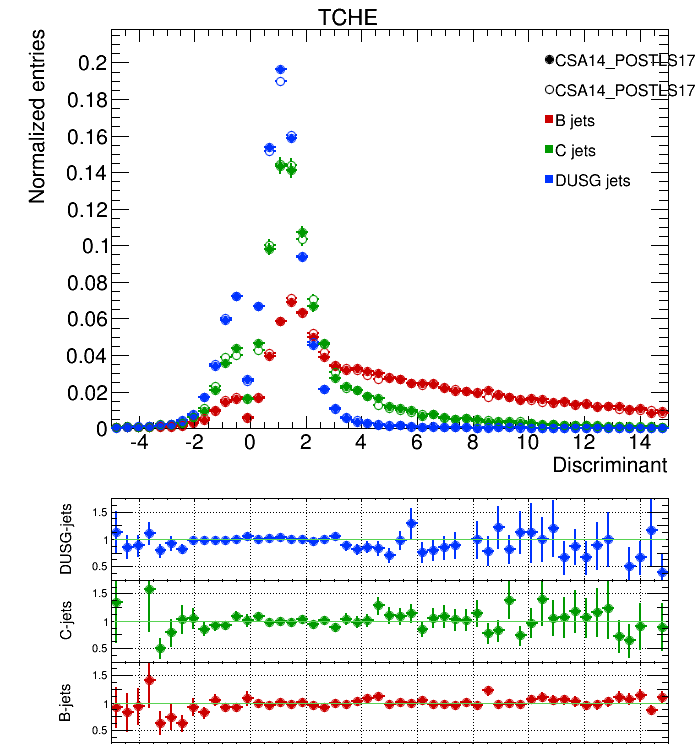
\includegraphics[width=0.49\textwidth]{bTagging/8TeV/TTbar_PU/TCHE_discr_GLOBAL_all}
        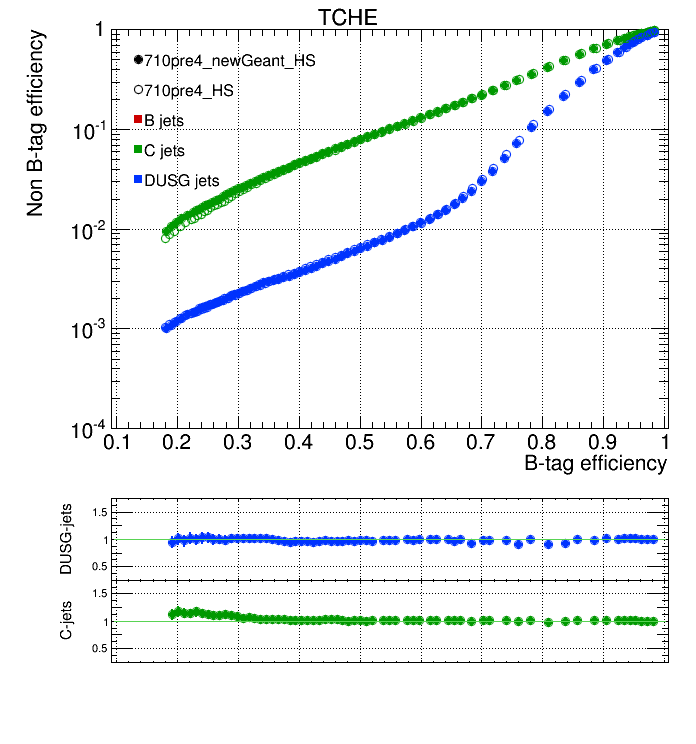
\includegraphics[width=0.49\textwidth]{bTagging/8TeV/TTbar_PU/TCHE_performance_vs_B_GLOBAL_all}
        \end{minipage}
        \caption{Superimposed discriminant distributions for light, $c$ and $b$ jets (on
        the left) and corresponding performances in term of misidentification rate versus $b$ jet efficiency
        (on the right) for the track counting high efficiency algorithm.
        The distribution and performances were estimated using the validation framework and from
        a $t\bar{t}$ sample in 8 TeV conditions, including pile-up.}
        \label{fig:bTagging/perfTC}
    \end{figure}

        \subsubsection{Jet probability}

    A more elaborate technique, but still based on track information alone, consists in
    using the impact parameter significance of
    several tracks in the jet. This can be done by computing a likelihood that all tracks
    associated to the jet originate from the primary vertex. The starting point for this
    is to know the distribution of $S_\text{IP}$ for prompt tracks and to compute, for
    each given track with impact parameter significance $X$, the probability $P_\text{track} =
    P(S_\text{IP} > X)$. To protect the algorithm from single, poorly reconstructed tracks,
    a lower bound is put on $P_\text{track}$ at 0.005. The probability $P_\text{jet}$ is
    then computed with the likelihood estimator, using the $N$ tracks of the jet,

    \eq{JPlikelihood}
    {
        P_\text{jet} = \Pi \cdot \sum_{i=0}^{N-1} \frac{(-\text{ln } \Pi)^i}{i!} \text{,\hspace*{0.6cm} with \hspace*{0.6cm}} \Pi = \prod_{i=1}^{N} \text{max}(P_{\text{track }i},0.005)
    }

    The jet probability (JP) discriminant is finally defined as $- \text{ln} P_\text{jet}$
    to have a convenient range to work with. An alternative version of this algorithm is
    called jet $B$ probability (JBP) and uses only the four tracks with highest $S_\text{IP}$.

    \reffig{fig:bTagging/perfJP} presents the discriminant and
    performances for the different jet categories for the jet probability algorithm. The
    small spikes in the discriminant distribution, also visible in the performance curves,
    come from the lower bound on $P_\text{track}$. The $b$ jet efficiencies are around
    81\%, 55\% and 39\% for the loose, medium and tight working points respectively.

    \begin{figure}[th!]
        \centering
        \begin{minipage}{\textwidth}
        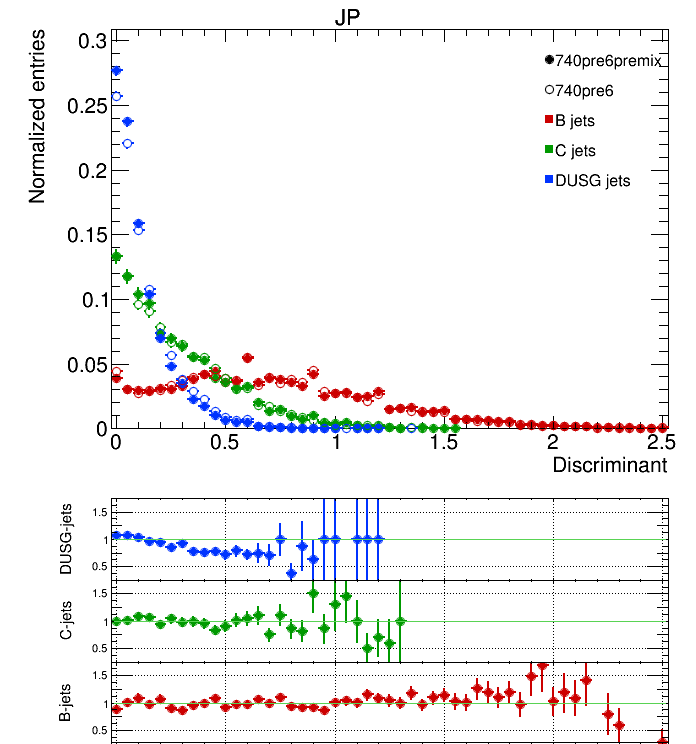
\includegraphics[width=0.49\textwidth]{bTagging/8TeV/TTbar_PU/JP_discr_GLOBAL_all}
        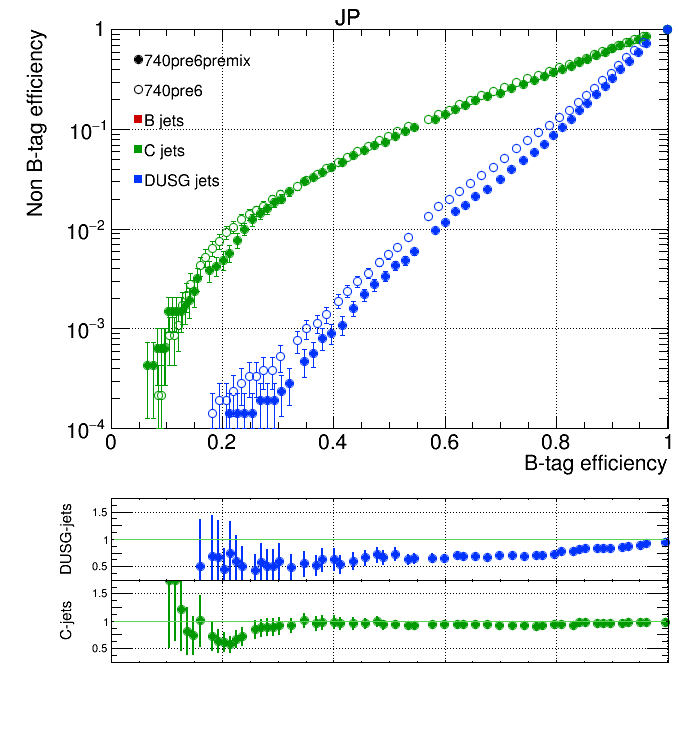
\includegraphics[width=0.49\textwidth]{bTagging/8TeV/TTbar_PU/JP_performance_vs_B_GLOBAL_all}
        \end{minipage}
                \caption{Superimposed discriminant distributions for light, $c$ and $b$ jets (on
        the left) and corresponding performances in term of misidentification rate versus $b$ jet efficiency
        (on the right) for the jet probability algorithm.
        The distribution and performances were estimated using the validation framework and from
        a $t\bar{t}$ sample in 8 TeV conditions, including pile-up.}
        \label{fig:bTagging/perfJP}
    \end{figure}

        \subsubsection{Simple secondary vertex}

    The simple secondary vertex (SSV) algorithm is based on secondary vertex reconstruction,
    and in particular uses the largest flight distance significance, among all secondary
    vertices associated to the jet, as a discriminant. As for the track counting algorithm, two versions are defined
    to obtain either high efficiency (SSVHE) using secondary vertices with at least two
    tracks, either high purity (SSVHP) which requires at least three tracks.

    \reffig{fig:bTagging/perfSSV} presents the discriminant and
    performances for the different jet categories for the high efficiency of this algorithm.
    The maximum efficiency achievable is limited by the intrinsic efficiency of
    actually finding a secondary vertex which satisfies the constraints. For this version,
    it is around 62\% for $b$ jets and 20\% for $c$ jets, while the fake vertices rate (i.e.
    probability to find a vertex in light jets) is around 2\%. The $b$ jet efficiencies
    for the medium and tight working points are around 58\% and 20\% respectively.

    \begin{figure}[th!]
        \centering
        \begin{minipage}{\textwidth}
        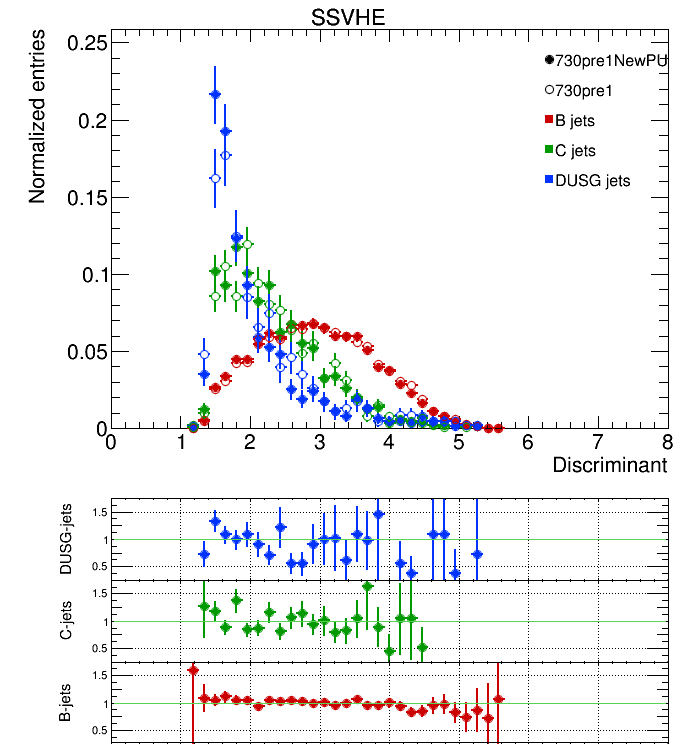
\includegraphics[width=0.49\textwidth]{bTagging/8TeV/TTbar_PU/SSVHE_discr_GLOBAL_all}
        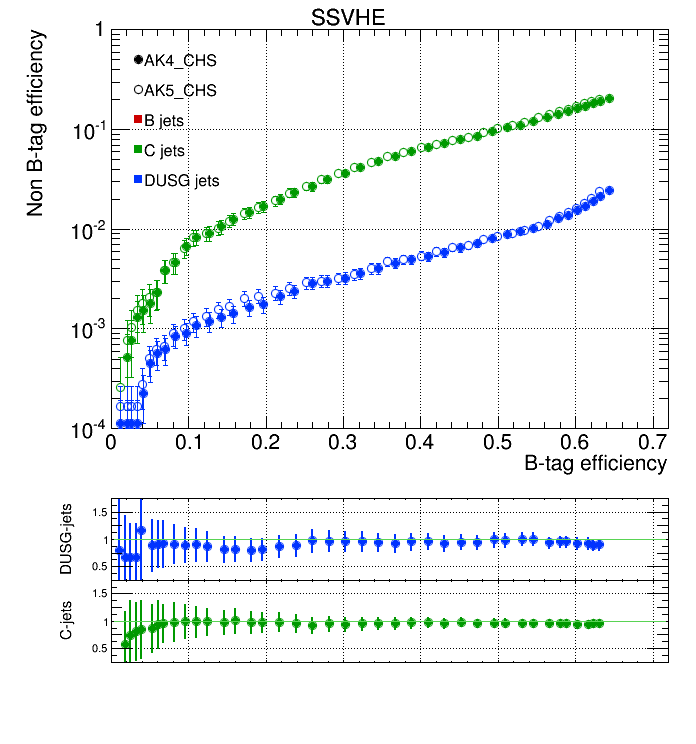
\includegraphics[width=0.49\textwidth]{bTagging/8TeV/TTbar_PU/SSVHE_performance_vs_B_GLOBAL_all}
        \end{minipage}
        \caption{Superimposed discriminant distributions for light, $c$ and $b$ jets (on
        the left) and corresponding performances in term of misidentification rate versus $b$ jet efficiency
        (on the right) for the simple secondary vertex high efficiency algorithm.
        The distribution and performances were estimated using the validation framework and from
        a $t\bar{t}$ sample in 8 TeV conditions, including pile-up.}
        \label{fig:bTagging/perfSSV}
    \end{figure}

        \subsubsection{Soft leptons algorithms}

    One can target the $b$ jets containing soft leptons with dedicated algorithms. However,
    as no observable exhibits a strong discriminating power alone, a multivariate analysis
    has to be used. Several discriminating observables are fed into a neural network
    which is trained to differentiate signal jets ($b$ jets) from background jets (light jets).
    These observables include $p_T^\text{rel.}$, the $\Delta R$ between the lepton and
    jet axis, the relative lepton momentum, the impact parameter significance of the lepton
    and the lepton quality. Two algorithms are defined, targeting either jets with a
    muon (soft muon tagger, SMT) or an electron (soft electron tagger, SET). While muons are
    well-identified objects because they leave a distinct signal in the muon system,
    electrons are more challenging due to the hadronic environment and dedicated in-jet
    electron identification must be defined. The maximum efficiency achievable for each
    lepton flavor tagger is intrinsically limited by the leptonic branching ratio of $B$ hadrons,
    which is about 20\% per flavor.

    In practice, the maximum $b$ jet efficiency for the soft electron tagger is around
    14\% compared to around 17\% for the soft muon tagger.
    \reffig{fig:bTagging/perfSMT} presents the discriminant and performances of the
    SMT algorithm. The $b$ jet efficiencies at medium and tight working points are around
    10\% and 7\% respectively.

    \begin{figure}[th!]
        \centering
        \begin{minipage}{\textwidth}
        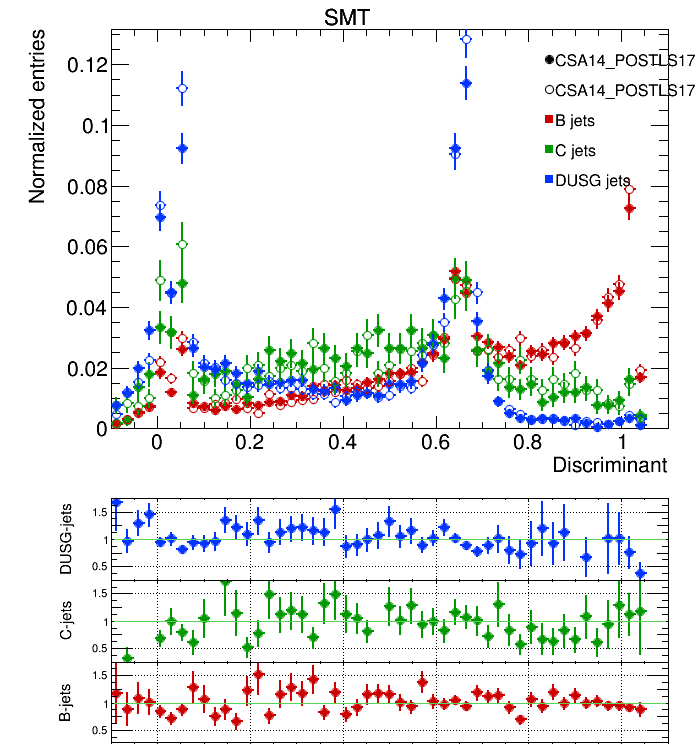
\includegraphics[width=0.49\textwidth]{bTagging/8TeV/TTbar_PU/SMT_discr_GLOBAL_all}
        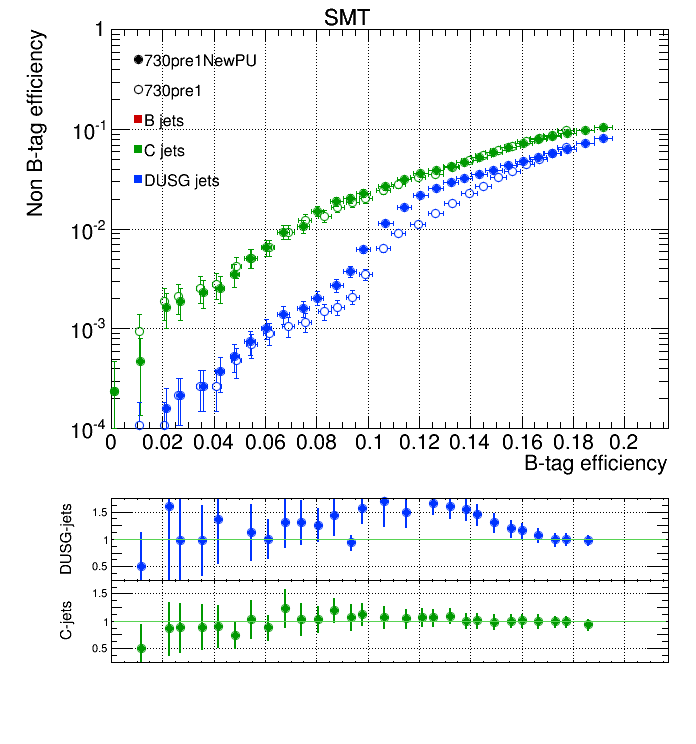
\includegraphics[width=0.49\textwidth]{bTagging/8TeV/TTbar_PU/SMT_performance_vs_B_GLOBAL_all}
        \end{minipage}
        \caption{Superimposed discriminant distributions for light, $c$ and $b$ jets (on
        the left) and corresponding performances in term of misidentification rate versus $b$ jet efficiency
        (on the right) for the soft muon algorithm.
        The distribution and performances were estimated using the validation framework and from
        a $t\bar{t}$ sample in 8 TeV conditions, including pile-up.}
        \label{fig:bTagging/perfSMT}
    \end{figure}

        \subsubsection{Combined secondary vertex}

    Finally, one may want to combine the techniques previously described as they complement
    each other. During the Run I, the track-based and secondary-based approach have been
    successfully combined into a combined secondary vertex algorithm (CSV). Developments are ongoing
    to include the soft lepton approaches in a new algorithm to be used during Run II.
    The CSV algorithm starts by dividing jets into categories according to whether or not a secondary
    vertex has been reconstructed. An intermediate category is designed for jets
    with no vertex fit but with still two tracks with $S_\text{IP} > 2$, which are used to
    define a pseudo-vertex in 15\% of the cases where no vertex is found for $b$ jets.
    With the goal of improving the rejection against $c$ jets, for jets with a vertex or pseudo-vertex,
    the tracks are ordered according to their impact parameter significance, and the
    $S_\text{IP}$ of the first track to raises the invariant mass of the vertex above
    the charm threshold ($1.5 \GeV$) acts as an additional good discriminating variable.

    Likelihoods are trained as function of $\pT$ and $\abseta$, and based on the secondary vertex information, the energy
    and rapidity distribution of the tracks at the secondary vertex compared to the remaining
    tracks in the jet, as well as the $S_\text{IP}$ of each track. Two likelihood ratios
    are defined, one to discriminate between light jets and $b$ jets, and the other between
    $c$ jets and $b$ jets.
    These likelihoods are then combined by weighting them with a factor 0.75 and 0.25
    respectively, accordingly to the typical needs of physics analyses.

    \reffig{fig:bTagging/perfCSV} presents the discriminant and
    performances of the CSV algorithm. At the loose working point, the $b$ jet efficiency is
    around 78\%, close to the track counting high efficiency algorithm. The $b$ jet efficiency
    at the medium working point is around 65\%, significantly better than track counting,
    simple secondary vertex and jet probability due to the completeness of the combined
    secondary vertex approach. The tight working point has a $b$ jet efficiency of 40\%,
    comparable to the jet probability algorithm.

    \begin{figure}[th!]
        \centering
        \begin{minipage}{\textwidth}
        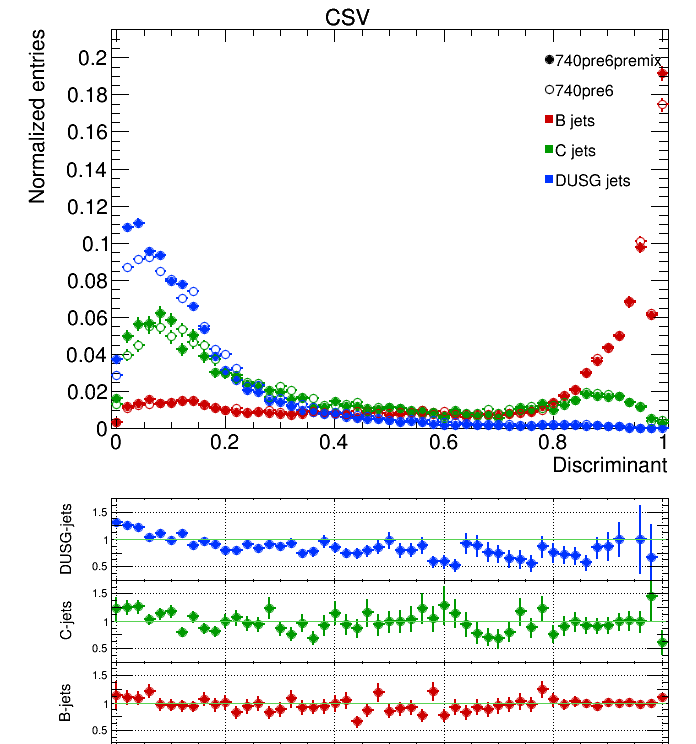
\includegraphics[width=0.49\textwidth]{bTagging/8TeV/TTbar_PU/CSV_discr_GLOBAL_all}
        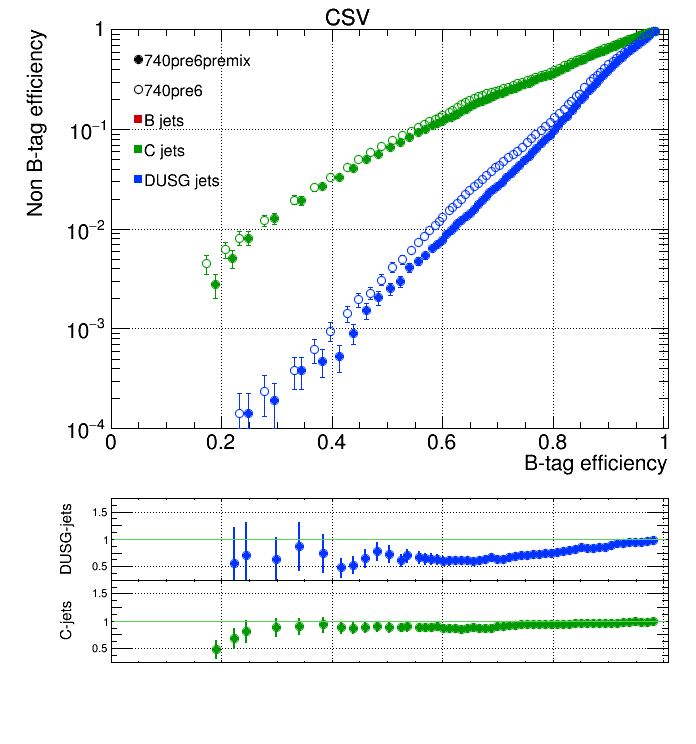
\includegraphics[width=0.49\textwidth]{bTagging/8TeV/TTbar_PU/CSV_performance_vs_B_GLOBAL_all}
        \end{minipage}
        \caption{Superimposed discriminant distributions for light, $c$ and $b$ jets (on
        the left) and corresponding performances in term of misidentification rate versus $b$ jet efficiency
        (on the right) for the combined secondary vertex algorithm.
        The distribution and performances were estimated using the validation framework and from
        a $t\bar{t}$ sample in 8 TeV conditions, including pile-up.}
        \label{fig:bTagging/perfCSV}
    \end{figure}

    \section{$b$-tagging validation in the CMS collaboration \label{sec:bTagValidation}}

    In this section, we focus on the contributions on $b$-tagging during this thesis.
    After presenting the context of the work and discussing statistical aspects, some
    important validations are presented in particular related to the preparation of the
    Run II of the LHC, while the last subsection is dedicated to a preliminary study of
    the Phase 2 conditions.

        \subsection{Context and validation method}

    The software of the CMS collaboration is constantly evolving. The development cycle
    includes rigorous and recurring checks by all the detector groups, physics
    object groups and analysis groups. The frequency of such a validation procedure
    of the software ensures an early identification of bugs and to understand
    the evolution of distributions and performances. The types of changes in the CMS
    software include, but are not limited to:
    \begin{itemize}
        \item \textbf{Versions of dependencies} such as \textsc{Geant4} and
              \textsc{Root} which may in turn impact the description of particle-matter
              interaction or statistical aspects.
        \item \textbf{Generators and simulation workflow}, for instance related to
              the tunning of the parton shower software, or the simulation of pile-up.
        \item \textbf{Detector geometry and description}, which is likely to change during
              long shutdowns, as subdetectors have been and will be upgraded.
        \item \textbf{Alignment and calibration conditions} can be tuned for instance to
              simulate early data-taking with misaligned tracker layers.
        \item \textbf{Reconstruction techniques}, which are likely to evolve across time to include
              new methods, tune parameters or optimize performances.
    \end{itemize}

    In particular, $b$-tagging algorithms are highly dependent on $B$ hadron modeling, tracking
    aspects, jet reconstruction and pile-up conditions.

    The validation activity consists in comparing typical $b$-tagging variables and performances
    between a new version and an older one, the reference. The reference is usually taken to
    be the previous version to only consider the changes introduced in the new version.
    One can estimate the $b$-tagging performances for the two versions and check their
    compatibility.

    \subsection{Sample size and impact on performance estimation}

    The validation work is made on four different samples in order to cross-check results
    and factorize the impact of pile-up or simulation type:
    \begin{itemize}
        \item a $t\bar{t}$ sample with pile-up, and full simulation of the detector
        \item a $t\bar{t}$ sample without pile-up, and full simulation of the detector
        \item a $t\bar{t}$ sample without pile-up, and fast simulation of the detector
        \item a QCD sample with $50 < \hat{\pT} < 120\GeV$, with $\hat{\pT}$ characterizing
            the energy of the process, and full simulation of the detector
    \end{itemize}

    As the validation is a recurrent process and the production of samples takes CPU
    resources and disk space, each sample contains only about 9000 events. This constraint
    impacts directly the magnitude of statistical fluctuations one will observe in
    variable distributions and in the performance estimation, in turn affecting the check of compatibility
    between the two versions.

    The compatibility of the two versions, the release to be validated (val.) and the
    reference (ref.), can be quantified in the following way. The efficiency for a given
    cut on the discriminant is computed in both versions and yields the corresponding
    values $\epsilon_\text{val.}$ and $\epsilon_\text{ref.}$ with relative uncertainty
    $\sigma^\text{rel.}_\epsilon$. The ratio $r \definedAs \epsilon_\text{val.}/\epsilon_\text{ref.}$
    is computed, and one wants to check if the ratio is significantly different from 1.
    The relative uncertainty on this ratio is $\sigma^\text{rel.}_r = \sqrt{2} \cdot \sigma^\text{rel.}_\epsilon$,
    assuming that $\epsilon_\text{val.}$ and $\epsilon_\text{ref.}$ are uncorrelated.

    To get an idea of the sensitivity of the validation, let's investigate what are the
    conditions to be able to see effects of magnitude lower than 20\% on $\epsilon$ at 2
    sigma level. We want $2 \cdot \sigma^\text{rel.}_r < 0.2$, and therefore approximately
    $\sigma^\text{rel.}_\epsilon < 7\%$. Considering the efficiency estimate $\epsilon
    = k/n$ from observing $k$ objects passing a selection among $n$, one can define a
    critical efficiency such that the relative uncertainty on the efficiency estimation
    will be higher than 7\%:

    \eq{criticalEfficiency}
    {
        \sigma^\text{rel.}_\epsilon = \frac{\sigma_\epsilon}{\epsilon} = \sqrt{\frac{1}{N} \frac{1-\epsilon}{\epsilon}} > 0.07
        \hspace*{1cm}
        \Rightarrow
        \hspace*{1cm}
        \epsilon < \frac{1}{\frac{N}{200} + 1}
    }

    \reftab{tab:criticalEfficiencyBTag} presents the number of jets according to their flavor,
    for the QCD and $t\bar{t}$ samples, as well as the critical efficiency associated
    to these numbers. This efficiency is about 1\% for light jets, meaning that effects
    lower than 20\% won't be distinguishable (at 2$\sigma$ level) from statistical
    fluctuations below the medium working point.

    \begin{table}
    \centering
    \begin{tabular}{|c|cc|cc|}
        \hline
                         & \multicolumn{2}{c}{QCD sample} & \multicolumn{2}{c}{$t\bar{t}$ sample} \\
        \hline
           Jet category  & Number & Critical efficiency   & Number & Critical efficiency \\
        \hline
            $u,d,s,g$    & 17000  & 1.2\%                 & 19600  & 1.0\% \\
            $c$          & 1400   & 12\%                  & 4500   & 4\%   \\
            $b$          & 700    & 22\%                  & 13000  & 1.5\% \\
        \hline
    \end{tabular}
        \caption{Typical number of selected jets, per flavor category and for two sample types,
        and critical efficiency below which effects lower than 20\% cannot be distinguished from
        statistical fluctuations at 2$\sigma$ level. \label{tab:criticalEfficiencyBTag}}
    \end{table}

    To avoid this problem, some validations, only intended to study the impact of new
    reconstruction techniques and algorithms, recycle the Monte-Carlo generation and detector simulation
    steps of previous validation samples, in order to remove the statistical fluctuations
    coming from these steps.

    \subsection{Validation of the new jet size parameter for the Run II}

    The preparation of the Run II of the LHC involves a change in the jet size parameter.
    Because the jets are expected to be narrower on average due to the energy increase,
    and to limit the pile-up contamination, this parameter is moved from $R = 0.5$ to $0.4$.

    The validation of this change is made using two sets of samples using the same
    generated events and the same simulation to limit the effect of statistical fluctuations,
    but reconstruction is done with the two different jet size parameters. The sample
    used to produce the following figures is a $t\bar{t}$ sample at $\sqrt{s} = 13\TeV$
    with pile-up.

    A comparison of the jets $\pT$ and $\eta$ spectra between the two reconstructions
    is presented on \reffig{fig:bTagging/AK4vsAK5/TTbar_FullSim_PU_kinematic}. The
    $\eta$ response is quite identical. However, small differences are seen in the $\pT$
    spectrum which are interpreted as coming from the jet energy corrections in the
    $R = 0.4$ reconstruction being still preliminary.

    \insertTwoFigures{bTagging/AK4vsAK5/TTbar_FullSim_PU_kinematic}
                     {bTagging/AK4vsAK5/TTbar_FullSim_PU/2_CSV_jetPt_GLOBAL_all}
                     {bTagging/AK4vsAK5/TTbar_FullSim_PU/4_CSV_jetEta_GLOBAL_all}
                     {0.49}
                     {Comparison of the $\pT$ (left) and $\eta$ (right) spectrum of
                     the selected jets in the context of the validation of the new
                     jet size parameter for the Run II.}

    \reffig{fig:bTagging/AK4vsAK5/TTbar_FullSim_PU_lowLevelVariables} on the top left
    presents on the distribution of the $\Delta R$ between the tracks in the jet
    and the jet axis. Small differences are observed
    at low $\Delta R(\text{track},\text{jet axis})$, pointing towards tracks being slightly
    closer to jet axis in $R = 0.4$ compared to $R = 0.5$. This is interpreted as coming
    from the fact that the jet axis is more likely to be perturbed by particles near
    the edge of the cone with $R = 0.5$ compared to $0.4$.
    On the top right, the comparison is done for the ratio of the energy of the sum
    of the tracks and the jet energy. This distribution exhibits a clear shift towards
    1 for $R = 0.4$ compared to 0.5. This is interpreted as coming from the fact that
    the selected tracks (i.e. in $R < 0.3$) represents a more significant fraction of
    the total jet energy in $R = 0.4$ compared to 0.5.

    \insertFourFigures{bTagging/AK4vsAK5/TTbar_FullSim_PU_lowLevelVariables}
                      {bTagging/AK4vsAK5/TTbar_FullSim_PU_lowLevelVariables/CSVTag_trackDeltaR_GLOBAL_all}
                      {bTagging/AK4vsAK5/TTbar_FullSim_PU_lowLevelVariables/CSVTag_trackSumJetEtRatio_GLOBAL_all}
                      {bTagging/AK4vsAK5/TTbar_FullSim_PU_lowLevelVariables/IPTag_ips_3D_GLOBAL_all}
                      {bTagging/AK4vsAK5/TTbar_FullSim_PU_lowLevelVariables/CSVTag_flightDistance3dSig_GLOBAL_all}
                      {0.49}
                      {Comparison of the $\Delta R(\text{track},\text{jet axis})$ (top left),
                      the ratio of track sum energy to jet energy (top right), the impact parameter
                      significance (bottom left) and the flight distance significance of the
                      secondary vertex (bottom right) in the context of the validation
                      of the new jet size parameter for the Run II. On the bottom of the plots,
                      the histogram corresponds
                      to the ratio of the distribution between $R = 0.4$ and $R = 0.5$.}

    Two other $b$-tagging variables are presented on the bottom of
    \reffig{fig:bTagging/AK4vsAK5/TTbar_FullSim_PU_lowLevelVariables}, namely the
    impact parameter significance and the flight distance of secondary vertices. Overall,
    a little improvement is observed in the distribution of the impact parameter significance
    for $b$ jets as a lower fraction of the tracks ends up with negative values. The
    flight distance of secondary vertices is stable.

    \insertFourFigures{bTagging/AK4vsAK5/TTbar_FullSim_PU_performances}
                      {bTagging/AK4vsAK5/TTbar_FullSim_PU/TCHE_performance_vs_B_GLOBAL_all}
                      {bTagging/AK4vsAK5/TTbar_FullSim_PU/JP_performance_vs_B_GLOBAL_all}
                      {bTagging/AK4vsAK5/TTbar_FullSim_PU/SSVHE_performance_vs_B_GLOBAL_all}
                      {bTagging/AK4vsAK5/TTbar_FullSim_PU/CSV_performance_vs_B_GLOBAL_all}
                      {0.49}
                      {Comparison of the algorithm performances for the track counting high
                      efficiency (top left), jet probability (top right), simple
                      secondary vertex (bottom left) and combined secondary vertex
                      (bottom right) in the context of the validation of the new jet size
                      parameter for the Run II. On the bottom of the plots, the histogram corresponds
                      to the ratio of the distribution between $R = 0.4$ and $R = 0.5$.
                      }

    The impact on the performances is presented on \reffig{fig:bTagging/AK4vsAK5/TTbar_FullSim_PU_performances}
    for four algorithms, TCHE, JP, SSVHE and CSV. The performances for TCHE and SSVHE
    are relatively stable while JP, dependent on the exact shape of the impact parameter
    significance for all tracks, has a $b$ jet efficiency improved by a few percents attributed to the
    observed small change in the impact parameter distribution. This also propagates to the
    performance of CSV where, at constant $b$ jet efficiency, the fake rate is lowered
    by about 20\%.

    To conclude, as the observations in this validation are well understood from a physics
    point of view and make sense, the change of jet size parameter has been validated for
    the $b$-tagging aspects.

    \subsection{Validation of new default pile-up rate for validation samples}

    As of the version v7.3.0 of the CMS software, the default pile-up rate for the validation
    samples was changed from 10 to 35. This should be differentiated from the pile-up rate
    used for analysis samples which follows a particular pile-up distribution.
    As tracking and $b$-tagging variables strongly depend on pile-up effects, this
    new condition is expected to impact significantly the performances.

    In this document, we investigate this change using a $t\bar{t}$ sample at $\sqrt{s} = 13\TeV$
    with pile-up. Because of the change in pile-up, the simulation step had to be performed
    separately for the two samples to be compared.

    \reffig{fig:bTagging/newPU35/tracking} compares the efficiency and fake rate of track
    reconstruction, as function of $\eta$, for a pile-up rate of 10 (\emph{old}) and
    35 (\emph{new}) \cite{TrackingNewPUComparison}. The new pile-up condition decreases the track reconstruction
    efficiency by about 2\% in the central region, and increases the fake rate from
    3\% to 8\%.

    \insertFigure{bTagging/newPU35/tracking}{0.99}{Comparison of the tracking
    performances as function of $\eta$ between the pile-up level of 10 (old) and 35 (new).
    The left plot shows the efficiency for real tracks while the right plot shows
    the fake and duplicate rate \cite{TrackingNewPUComparison}.}

    On the $b$-tagging side, this translates to more contamination from pile-up and
    fakes, likely to have large impact parameters or to create fake secondary vertices.
    \reffig{fig:bTagging/newPU35/lowLevelVariables} shows the comparison of the impact
    parameter significance and secondary vertex category between the two pile-up conditions.
    The impact parameter distribution for tracks in light jets gets a wider peak around
    0, from which we can expect an increase in fake rate for all algorithm based on
    this variable. The secondary vertex categorization shows also a 5\% absolute loss
    in vertexing efficiency for $b$ jets, and an relative increase of around 35\% for light
    jets containing a secondary vertex. From this, we can expect that algorithms based
    on secondary vertex reconstruction will not only suffer from a higher fake rate from
    light jets, but also a lower maximum efficiency for $b$ jets.

    \insertTwoFigures{bTagging/newPU35/lowLevelVariables}
                     {bTagging/newPU35/TTbar_730pre1NewPU_vs_730pre1_FullSim_PU25ns_lowLevelVariables/IPTag_ips_3D_GLOBAL_all}
                     {bTagging/newPU35/TTbar_730pre1NewPU_vs_730pre1_FullSim_PU25ns_lowLevelVariables/CSVTag_vertexCategory_GLOBAL_all}
                     {0.49}
                     {Comparison of the impact parameter significance (on the left)
                     and vertex category for the CSV algorithm (on the right) in the
                     context of the validation of the new default pile-up rate.}

    \reffig{fig:bTagging/newPU35/performances} presents the impact on the performances
    for the four main algorithms TCHE, JP, SSVHE and CSV. The overall impact is a higher
    fake rate from light jets by about 50\% and from $c$ jets by about 5-10\%. The
    maximum efficiency for $b$ jets for SSVHE is decreased by about 5\%, directly
    related to what is observed on the vertex category in \reffig{fig:bTagging/newPU35/lowLevelVariables}.

    \insertFourFigures{bTagging/newPU35/performances}
                      {bTagging/newPU35/TTbar_730pre1NewPU_vs_730pre1_FullSim_PU25ns/TCHE_performance_vs_B_GLOBAL_all}
                      {bTagging/newPU35/TTbar_730pre1NewPU_vs_730pre1_FullSim_PU25ns/JP_performance_vs_B_GLOBAL_all}
                      {bTagging/newPU35/TTbar_730pre1NewPU_vs_730pre1_FullSim_PU25ns/SSVHE_performance_vs_B_GLOBAL_all}
                      {bTagging/newPU35/TTbar_730pre1NewPU_vs_730pre1_FullSim_PU25ns/CSV_performance_vs_B_GLOBAL_all}
                      {0.49}
                      {Comparison of the algorithm performances for the track counting high
                      efficiency (top left), jet probability (top right), simple
                      secondary vertex (bottom left) and combined secondary vertex
                      (bottom right) in the context of the validation of the new pile-up
                      rate. On the bottom of the plots, the histogram corresponds
                      to the ratio of the distribution between $PU = 10$ and $PU = 35$.}

    \subsection{Validation of the premixing technique for pile-up simulation}

    In the CMS software v7 cycle, a new technique, called premixing, started being developed.
    The motivation for this technique starts from the observation that, when generating and
    simulating events, the simulation of the detector response to the pile-up represents
    a large fraction of the CPU time, compared to one single hard-scattering.

    In order to reduce the CPU cost of simulation, strategies can be developed. In the
    case of premixing, the idea is to factorize the simulation of the interaction of the particles with the
    detector, coming from on one hand, the pile-up, and on the other hand, the hard-scattering
    of interest. By doing so, the interaction of the pile-up particles can be computed once for
    all, and their contribution to the signal in the sensors can be overlaid to any
    hard-scattering event, drastically reducing the simulation time per event \cite{Premixing}.

    In order for this to work, one must however be careful regarding the way that the
    pile-up and hard-scattering are digitized and combined together. For instance,
    thresholds in the subdetectors (e.g. a given calorimetric tower), may
    impact the digitization such that the hard-scattering alone, or the pile-up alone,
    may not produce a significant signal, but the combination of the two may. To
    work around this problem, thresholds are initially set to zero when the digitization
    is done, and applied only after mixing of the pile-up with the hard-scattering.

    Overall, one wants the premixing technique to not impact the physics at the reconstruction
    level. $b$-tagging, as a high-level technique, is highly sensitive to the description
    of tracks and calorimeter deposits and therefore allows an overall check that premixing does
    not introduce any unphysical behavior. While there were several validations related to
    this work, this document focuses on a pathological validation done in version 7.4.0
    of the CMS software.

    Validation results are shown on \reffig{fig:bTagging/premixing/lowLevelVariables} from
    a $t\bar{t}$ sample with pile-up included and full simulation. The version of the
    premixing used led to tracks having an artificially higher number of hits in the
    pixels on average, and therefore a better track quality, which manifests as a lower
    tail for the normalized $\chi^2$ distribution, and overall a better resolution.
    This in turn impacts the number of tracks at the secondary vertex for light jets, and the
    impact parameter significance.

    \insertFourFigures{bTagging/premixing/lowLevelVariables}
                      {bTagging/premixing/TTbar_740pre6premix_vs_740pre6_FullSim_PU50ns_lowLevelVariables/IPTag_tkNPixelHits_3D_GLOBAL_all}
                      {bTagging/premixing/TTbar_740pre6premix_vs_740pre6_FullSim_PU50ns_lowLevelVariables/IPTag_tkNChiSqr_3D_GLOBAL_all}
                      {bTagging/premixing/TTbar_740pre6premix_vs_740pre6_FullSim_PU50ns_lowLevelVariables/CSVTag_vertexNTracks_GLOBAL_all}
                      {bTagging/premixing/TTbar_740pre6premix_vs_740pre6_FullSim_PU50ns_lowLevelVariables/IPTag_ips_3D_GLOBAL_all}
                      {0.49}
                      {Comparison of the number of pixel hits (top left), track $\chi^2$
                      (top right), number of tracks at the secondary vertex (bottom left) and
                      impact parameter significance (bottom right) in the context
                      of the premixing validation. On the bottom of the plots, the histogram corresponds
                      to the ratio of the distribution between premixing and standard mixing. }

    This impacts the performances of both impact parameter-based algorithms and
     secondary vertex-based algorithms significantly, as shown on
    \reffig{fig:bTagging/premixing/performances}: for TCHE, the fake rate from lights
    decreases by about 35\% at constant $b$ jet efficiency of 65\%, while SSVHE gets about 20\%
    lower fake rate from $c$ jets.

    \insertTwoFigures{bTagging/premixing/performances}
                     {bTagging/premixing/TTbar_740pre6premix_vs_740pre6_FullSim_PU50ns/TCHE_performance_vs_B_GLOBAL_all}
                     {bTagging/premixing/TTbar_740pre6premix_vs_740pre6_FullSim_PU50ns/SSVHE_performance_vs_B_GLOBAL_all}
                     {0.49}
                     {Comparison of the algorithm performances of track counting high
                      efficiency (left) and simple secondary vertex high efficiency (right).
                      On the bottom of the plots, the histogram corresponds
                      to the ratio of the distribution between premixing and standard mixing. }

    This validation has therefore contributed to the identification of the problems with
    this version of the premixing. Since then, premixing has been developed further and
    proved to be in agreement with the regular mixing, has been estimated to speed up the
    simulation by a factor 3 \cite{Premixing} and became part of the CMS workflow.

    \subsection{Studies of high pile-up scenario for Phase 2}

    This validation study relates to one of the early investigations of $b$-tagging at high
    pile-up rate ($\orderOf{150}$). Such conditions are
    foreseen for the high-luminosity LHC (HL-LHC) program, also called Phase 2, which
    should start around 2027. Such prospective work is therefore crucial to obtain a first
    idea of the performances of the detector in these conditions, anticipate possible
    problems and guide the orientation of the development for object reconstruction.

    The reference used for this validation is a $t\bar{t}$ sample generated with $\sqrt{s}
    = 14\TeV$. The detector is simulated with the expected geometry for Phase 1 with
    a pile-up of 50, and the conditions of the technical design report (TDR) \cite{Phase1TDR}. The
    comparison is made with a $t\bar{t}$ sample with a Phase 1 aged geometry and a pile-up
    of 140.

    \insertTwoFigures{bTagging/highPU/kinematic}
                     {bTagging/highPU/pT}
                     {bTagging/highPU/eta}
                     {0.49}
                     {Comparison of the $\pT$ and $\eta$ spectra of the selected jets
                     in the context of the studies of a high pile-up scenario for Phase 2.
                     On the bottom of the plots, the histogram corresponds
                     to the ratio of the distribution between the PU = 140 and PU = 50
                     scenario.
                     (Note that the color code is different from the previous plots.)}

    \reffig{fig:bTagging/highPU/kinematic} presents the comparison of the kinematic
    distributions of the jets between the two samples. The first observation is that the increase of pile-up
    significantly bias the $\pT$ spectrum of the jets towards higher values, while the
    generated energy of the underlying partons are expected to have the same spectrum
    between the two releases. This is interpreted as coming from the jet energy corrections
    which are not yet adapted for the pile-up conditions of Phase 2, and points to
    a necessity of improving the mitigation of pile-up in jet reconstruction in general.
    The higher pile-up rate also creates a significantly higher
    number of jets in the central region ($\abseta < 0.7$), contributing to the gluon jet
    category.

    \insertTwoFigures{bTagging/highPU/lowLevel}
                     {bTagging/highPU/nSelTracks}
                     {bTagging/highPU/ips}
                     {0.49}
                     {Comparison of the number of selected tracks per jet (left) and
                     impact parameter significance (right) in the context of the
                     studies of a high pile-up scenario for Phase 2.
                     On the bottom of the plots, the histogram corresponds
                     to the ratio of the distribution between the PU = 140 and PU = 50
                     scenario.
                     (Note that the color code is different from the previous plots.)
                     }

    \reffig{fig:bTagging/highPU/lowLevel} shows track level information, namely the
    distribution of the number of selected tracks per jet, and the distribution of the
    impact parameter significance for these tracks. In the high pile-up scenario, the
    number of selected tracks is significantly lower for all jets categories, interpreted
    as coming from the simulated aging of the pixel detector. In particular
    for the $b$ jet category, the distribution peaks around 7 or 8 selected tracks per
    jet in the Phase 2 scenario, compared to around 10 in the Phase 1. From this observation, one
    can expect a significant decrease in the $b$ jet efficiency. The distribution of
    the impact parameter significance also exhibits a worsening of the discriminating
    power. First, the distribution for light jets exhibits a much wider peak and
    increase of the fraction with large positive values. Secondly, the ratio of the
    distribution for the $b$ jets shows a trend in the positive-tail such that the
    distribution in high pile-up conditions is less in favor of $b$ jets discrimination.

    \insertFourFigures{bTagging/highPU/perf}
                      {bTagging/highPU/TCHEperf}
                      {bTagging/highPU/JPperf}
                      {bTagging/highPU/SSVHEperf}
                      {bTagging/highPU/CSVperf}
                      {0.49}
                      {Comparison of the performances for track counting high efficiency
                      (top left), jet probability (top right), simple secondary vertex
                      (bottom left) and combined secondary vertex
                      (bottom right) in the context of the studies of a high-pile-up
                      scenario for Phase 2. On the bottom of the plots, the histogram corresponds
                      to the ratio of the distribution between the PU = 140 and PU = 50
                      scenario. (Note that the color code is different from the previous plots.) }

    \reffig{fig:bTagging/highPU/perf} shows the comparison of the performances curves
    obtained for the two scenarios for the four main algorithms: track counting high
    efficiency, simple secondary vertex high efficiency, jet probability and combined secondary vertex.
    Track counting and jet probability, both relying essentially on the impact parameter
    significance distribution, show a dramatic increase of the fake rate by a factor
    5 to 10 in the high PU scenario. The maximum $b$ jet efficiency for simple secondary
    vertex is also significantly affected and gets down to about 55\%, while the fake rate
    for is only increased by a factor between 2 and 5. The combined secondary vertex
    performances finally give information to what can be expected from combining the
    techniques together. The fake rate for light jets is overall increased by a factor 5
    to 10 while it is increased by a factor 1.5-2 for $c$ jets. The $b$ jets efficiency in
    the high pile-up scenario becomes 65\%, 42\% and about 20\% for the loose, medium and
    tight working points respectively.

    \insertTwoFigures{bTagging/highPU/TP}
                     {bTagging/highPU/PVidentification}
                     {bTagging/highPU/CSVperf_2}
                     {0.49}
                     {On the left: comparison of the primary vertex choice efficiency as function of the
                     leading jet $\pT$, for different scenario corresponding to Phase 1
                     with a pile-up rate of 50 (blue squares),
                     Phase 1 aged detector with pile-up rate of 140 using the old (open
                     green triangles) or new (filled green triangles) vertex choice
                     technique, and Phase 2 detector with a pile-up rate of 140 (red dots).
                     On the right: comparison of the $b$-tagging performances for the same
                     scenarios, showing how the Phase 2 detector is able to recover performances
                     comparable to Phase 1 \cite{Phase2TDR}.}

    Moreover, all these algorithms (with a particular case for simple secondary vertex)
    shows a maximum $b$-tagging efficiency around 80-85\% which is much unexpected. This
    was later \cite{Phase2TDR} tracked down as coming from the misidentification of the right primary vertex
    in the event due to the high level of pile-up. We recall that the primary vertex
    is typically chosen as the vertex with higher $\sum_\text{tracks} \pT^2$. However,
    as shown on \reffig{fig:bTagging/highPU/TP} on the left in open green triangles, this
    technique becomes quite less efficient at high pile-up, with an efficiency between 80 and 90\%
    for events with a leading jet with $100 < \pT < 200 \GeV$. To solve this issue, a new
    technique has been developed. This technique starts by clustering tracks to create jets,
    and the choice of the primary vertex is based on $\sum_\text{jets} \pT^2$ (though also
    including unclustered tracks to the sum). This new technique allows to significantly
    recover the vertex choice efficiency as shown with filled green triangles.

    Furthermore, an investigation of the performances using this time the foreseen Phase 2
    geometry has been pursued. On \reffig{fig:bTagging/highPU/TP} on the right, the
    performances are compared for three scenarios, namely Phase 1 geometry with a pile-up
    rate of 50, aged Phase 1 geometry with a pile-up of 140, and Phase 2 geometry with
    a pile-up of 140. The Phase 2 geometry has been demonstrated to significantly reduce
    the fake rate from light jets to obtain performances comparable to Phase 1 with a
    pile-up rate of 50.

%==============================================================
\setcounter{mtc}{5}
\chapterwithnum{Search for stop pair production at $\sqrt{s} = 8\TeV$}
\vspace*{-0.7cm}
\begin{center}
\begin{minipage}{0.95\textwidth}
\emph{« There are worlds out there where the sky is burning, and the sea’s asleep, and the rivers dream;
people made of smoke and cities made of song. Somewhere there’s danger, somewhere there’s injustice,
and somewhere else the tea’s getting cold. Come on, Ace. We’ve got work to do. »}\\
\hspace*{0.75\textwidth} The Seventh Doctor
\end{minipage}
\end{center}

\minitoc
\newpage
%==============================================================

    This chapter focuses on an analysis performed within the CMS collaboration
    and searching for the production of stop pair using the data recorded during
    the Run I of the LHC at $\sqrt{s} = 8\TeV$. In \refsection{sec:analysis_contextAndPheno},
    we concentrate on the context and phenomenology of the signature while
    \refsection{sec:analysis_overview} to \refsection{sec:analysis_results} discuss
    the different aspects of the analysis itself, namely the object and event selection,
    the signal region design, the background estimation, the systematics uncertainties, and
    finally the results and their interpretation. In the last \refsection{sec:analysis_perspective},
    some of the perspectives for this analysis are investigated, in particular regarding
    the use of $W$-tagging, followed by a sensitivity estimation for the Run II.

    \section{Context and phenomenology \label{sec:analysis_contextAndPheno}}
    %==============================================================

    \subsection{Theoretical context and constraints}
    %==============================================================

    \subsubsection{Motivation and constraints on the stop sector from the Higgs sector}

    As introduced in \refsection{sec:SUSY}, one of the best assets of supersymmetry is its ability to explain why the Higgs
    boson can be light, via the boson-fermion symmetry which protects the mass
    of the Higgs from diverging because of quantum corrections. This is illustrated on
    \reffig{fig:higgsCorrections}, showing the one-loop corrections to $m_h^2$
    from a fermionic field $f$ and a bosonic field $b$ coupled to the Higgs via the
    Lagrangian terms $- \lambda_f h \bar{f} f$ and $\lambda_b \left| h \right|^2 \left| b \right|^2$.

    \insertTwoFigures{higgsCorrections}
    {feynmanDiagrams/output/higgsFermionCorrection}
    {feynmanDiagrams/output/higgsBosonCorrection}{0.4}
    {One-loop correction to the Higgs for a fermionic field $f$ (left) and a bosonic field $b$ (right).}

    The leading order corrections associated to these diagrams are:
    \begin{equation}
        \Delta \mass{h}^2 = - \frac{\left| \lambda_f \right|^2}{8\pi^2} \Lambda^2_{\text{UV}}
        \, \, \, \, \, \, \, \, \, \, \text{and} \, \, \, \, \, \, \, \, \, \,
        \Delta \mass{h}^2 =   \frac{\lambda_b}{16\pi^2} \Lambda^2_{\text{UV}}
    \end{equation}
    where $\Lambda^2_{\text{UV}}$ is the ultraviolet momentum cutoff which regulates
    the loop integral. In the most ideal case, one can have $\left| \lambda_f \right|^2
    = \lambda_b$, which corresponds to $\mass{f} = \mass{b}$, and associate two scalars
    to each fermion (one for each chirality) so that the corrections cancel each others.
    If the masses of $f$ and $b$ are not the same, however, the corrections do not
    perfectly cancel each other and tunning has to be reintroduced to keep the
    corrections to the Higgs mass low. Since the top quark has the biggest Yukawa coupling $\lambda$, a
    particular attention in supersymmetry goes into the study of its superpartner
    which is expected to play an important role in stabilizing the mass of the Higgs.

    One can study the level of tunning needed as a function of the mass of the superpartner
    of the top, called the stop, for the theory to keep providing a natural explanation to the hierarchy
    problem, and use it as a guidance for experimental searches. It is possible to quantify
    fine-tunning by studying how the quantity of interest, in our case $m_h$, the Higgs mass,
    varies as function of $p_i$, the parameters of the theory:
    \eq{fineTunning}
    {
        \Delta \mass{h}
        \definedAs
        \text{max}_i
        \left|
             \frac
             {\partial \text{ln}\, \mass{h}^2}
             {\partial \text{ln}\, p_i}
        \right|
    }
    Despite the fact that such a study is highly dependent on hypotheses made on the SUSY parameters,
    it is commonly admitted that stop quarks should have a mass below or around $1\TeV$
    for SUSY to remain natural \cite{TheMoreMinimalSSM, NaturalSusyEndures, ANaturalSUSYHiggs,NaturalSUSYAndDarkMatter}. This makes the search for
    stops an important channel to constrain naturalness or possibly discover SUSY
    at the LHC.

    In addition to the argument of naturalness, one may derive constraints on the stop
    sector directly from the knowledge of the Higgs mass \cite{TheLightStopWindow}. In
    the context of supersymmetry, the Higgs mass may indeed be expressed as function
    of the other parameters of the theory. Assuming that $\mass{A} \gg \mass{Z}$:
    \eq{higgsMassInSUSY}
    {
        \mass{h}^2
        =
        \mass{Z}^2 \text{cos}^2 2\beta
        +
        \frac{3 \lambda_t^2 \mass{t}^2}{4\pi^2}
        \left[
            \text{log} \left( \frac{\mass{S}^2}{\mass{t}^2} \right)
            +
            X_t^2 \left( 1 - \frac{X_t^2}{12} \right)
        \right]
        + ...
    }
    where here, $X_t$, the stop mixing parameter, is defined as
    $(A_t + \mu\, \text{cot} \beta) / \mass{S}$ and $\mass{S} \definedAs
    \sqrt{\mass{\tilde{t}_1}\mass{\tilde{t}_2}}$ is the average stop
    mass. From this computation, constraints can be put on the value of $\mass{S}$ as
    function of $X_t$, as shown on the left of \reffig{fig:stopSectorConstraints} when assuming $\tan\, \beta
    = 20$. For $\mass{h}= 125\GeV$, one finds that the minimum value of $\mass{S}$ is
    around $600\GeV$, obtained for the so-called maximal mixing value $X_t = \sqrt{6}$.
    Interestingly, the observed Higgs mass therefore points to relatively ``heavy''
    stops compared to the naturalness argument favoring light stops.

    \insertTwoFigures{stopSectorConstraints}
                     {theory/averageStopMassConstraint}
                     {theory/constraintsFromHgg}
                     {0.49}
                     {Constraints on the stop sector from the Higgs measurement \cite{TheLightStopWindow}.
                     On the left, constraints on $\mass{S}$ as function of $X_t$ from
                     for different values of the Higgs mass. On the right, constraints
                     in the $(\mass{\tilde{t}_1},\mass{\tilde{t}_2})$ space: the
                     red area is forbidden because, as seen on the left plot, $m_S$
                     should be higher than about $600\GeV$ for $\mass{h} = 125\GeV$ ;
                     the lines corresponds to a few different values of $\Delta_t$,
                     namely -0.05, 0, 0.05 and 0.1, with $X_t^2 > 6$ (in blue) or
                     $X_t^2 < 6$ (in black).
                     }

    Moreover, it is remarkable that constraints on the stop sector can also be derived
    from the loop to the decay $h \rightarrow gg$ and $h \rightarrow \gamma \gamma$
    as described in \cite{TheLightStopWindow}. As the photon is not massive,
    the decay $h \rightarrow \gamma \gamma$ must involve virtual loops of massive
    particles, such as the top, but also possibly its superpartner the stop which
    would then affect the branching ratio $\text{BR}(h \rightarrow \gamma\gamma)$.
    The impact can be expressed as function of the stop sector parameters $\mass{S}$,
    $X_t$, $\mass{\tilde{t}_1}$ and $\mass{\tilde{t}_2}$:
    \eq{higgsGammaGammaStopConstraint}
    {
        \frac{\text{BR}(h\rightarrow\gamma\gamma)}{\text{BR}(h\rightarrow\gamma\gamma)_\text{SM}}
        =
        (1 - 0.28 \Delta_t)^2
        \hspace*{0.5cm}
        \text{with}
        \hspace*{0.5cm}
        \Delta_t
        \approx
        \frac{\mass{t}^2}{4}
        \left(
            \frac{1}{\mass{\tilde{t}_1}^2}
            +
            \frac{1}{\mass{\tilde{t}_2}^2}
            -
            \frac{X_t^2}{\mass{S}^2}
        \right).
    }

    At this point, the experimental measurement of $\text{BR}(h\rightarrow\gamma\gamma)$
    does not allow to significantly constrain the value of $\Delta_t$. Nevertheless,
    the lines in the right plot of \reffig{fig:stopSectorConstraints} plot illustrate
    how given values of $\Delta_t$ would in turn constrain the
    $(\mass{\tilde{t}_1},\mass{\tilde{t}_2})$ space.

    \subsubsection{Motivation from the dark matter evidence}

    A second appealing feature of supersymmetry is that it provides dark matter
    candidates. This happens in particular in R-parity conserving models, where the
    lightest supersymmetric particle (LSP) is a good dark matter candidate if it is
    not a charged particle. In the context of the MSSM, the lightest neutralino
    $\lneutralino$, the gravitino $\tilde{G}$ and the lightest sneutrino $\tilde{\nu}$
    can be the LSP. The lightest neutralino is the one that is most often studied as its
    relation to the electroweak sector makes it a perfect WIMP candidate.
    An advantage of the WIMP phenomenology is that their relic density can be calculated
    precisely in the framework of standard cosmology, assuming that they are thermally produced
    \cite{EllisDarkMatter}.
    Moreover, the naturalness argument also motivates the Higgsino mass $\mu$ to be around
    $150-200\GeV$ \cite{NaturalSUSYAndDarkMatter}. Following this, it means that the first
    neutralinos should be relatively light, and though the exact constraint
    depend on assumptions on $\text{tan}\, \beta$, $M_1$ and $M_2$, it is reasonable to
    consider that the lightest neutralino should be lighter than around $500\GeV$.
    Scenarios with a sneutrino as LSP might be studied as well, in particular in models
    attempting to explain the mass of the neutrinos, while the gravitino as LSP appears
    in gravity mediated SUSY breaking models.

    \subsection{Phenomenology and signature \label{sec:phenoAndSignature}}
    %=======================================

    In the context of this document, we focus on a SUSY spectra built from the
    previous arguments, which motivates a stop $\lstop$ with a mass lower than around
    $1\TeV$ and a dark matter candidate, which we take to be the lightest neutralino
    $\lneutralino$ assumed to be the LSP. While we could simply concentrate on these
    two particles, we will also consider cases where the lightest chargino $\lchargino$
    is the NLSP, i.e. has a mass higher than the neutralino $\lneutralino$ but lower
    than the stop $\lstop$. The $\lchargino$ is indeed expected to have a mass close
    to the $\lneutralino$ when the SUSY parameters $M_1$ and $M_2$
    are large compared to $\mu$. Experimentally, we now want to look for this particle
    spectrum via a search for a direct pair production of $\lstop$ in the $pp$ collisions of the LHC.

    As it is in practice impossible to perform such a search across the whole phase
    space of SUSY models, a pragmatic approach often consists in using simplified SUSY
    models where an
    effective Lagrangian introduces a limited set of new physics features. In such
    simplified models, the free parameters are usually taken to be experimentally
    meaningful quantities, such as the masses of the SUSY particles. This makes
    it possible for experimental searches to produce generic results that can later
    be reinterpreted in specific realizations of SUSY \cite{LiemSMS, SmodelS}
    or other BSM theories. In our case, let's consider the existence of only three new
    particles\footnote{The remaining SUSY particles can be assumed to be too heavy to
    have any significant impact on what is discussed here.}: the lightest stop quark
    $\lstop$, the lightest neutralino $\lneutralino$ and the lightest chargino $
    \lchargino$.

    First, let's assume that $\mass{\lchargino} \gg \mass{\lstop}$ and therefore the
    stop decays through $\lstop \rightarrow t \lneutralino$, as represented on
    \reffig{fig:stopDecayModes} on the left. This signal is referred to as \textsc{T2tt}
    in the simplified model nomenclature and depends on two free parameters
    $\mass{\lstop}$ and $\mass{\lneutralino}$.

    A second case is considered with $\mass{\lchargino} \in [\mass{\lneutralino},
    \mass{\lstop}]$ and the stop decays through $\lstop \rightarrow b \lchargino
    \rightarrow b W^{\pm} \lneutralino$. This signal is referred to as \textsc{T2bw}
    in the simplified model nomenclature. In addition to the free  parameters
    $\mass{\lstop}$ and $\mass{\lneutralino}$, $\mass{\lchargino}$ is set through a
    third parameter $x$ defined such that $\mass{\lchargino} = x \cdot \mass{\lstop}
    + (1 - x) \cdot \mass{\lneutralino}$. We study three cases $x = 0.75$, $0.50$
    and $0.25$, as represented on \reffig{fig:stopDecayModes} on the right.

    \insertFigure{stopDecayModes}{0.8}
                 {Representation of the mass hierarchy in the $\lstop \rightarrow t
                 \lneutralino$ decay mode (on the left) and $\lstop \rightarrow b
                 \lchargino \rightarrow b W^{\pm} \lneutralino $ decay mode (on the
                 right). For the later, the chargino mass $\mass{\lchargino}$ is
                 parametrized using $\mass{\lchargino} = x \cdot \mass{\lstop}
                 + (1 - x) \cdot \mass{\lneutralino}$ and three different values of $x$
                 are studied, $x = 0.75$, $0.50$ and $0.25$.}

    All of these four decay hypotheses are studied independently
    of each other\footnote{We do not consider mixed decays where one stop of the pair
    decays through $\lstop \rightarrow t \lneutralino$ and the other decays through
    $\lstop \rightarrow b \lchargino \rightarrow b W^{\pm} \lneutralino$.} and with a
    branching ratio equal to 1. It should also be noted that the polarization of the
    top quarks in the $\lstop \rightarrow t \lneutralino$ mode, and $\lchargino$ and
    $W$ bosons in the $\lstop \rightarrow b \lchargino \rightarrow b W^{\pm}
    \lneutralino$ mode, are dependent on the mixing matrices of the $\lstop$, $\lchargino$
    and $\lneutralino$. This can later significantly affect the distributions of
    variables and the acceptance of the signal, and is discussed during the
    interpretation of the results in \refsection{sec:analysis_results}.

    \reffig{fig:stopFeynmanDiagrams} shows the two Feynman diagrams that are
    considered. It is relevant to target both those signals with the same analysis
    considering that, in \textsc{T2tt}, the top quark almost exclusively decays
    through $t \rightarrow b W^+$ and therefore lead to the same intermediate state
    $b \bar{b} W^+ W^- + \lneutralino \lneutralino$ as in \textsc{T2bw}. Because the
    $\lneutralino$ are assumed to be dark matter candidates and do not interact with
    the detector, the signature left by this new physics process is a final state much
    like Standard Model $t\bar{t}$ production but with extra missing transverse energy
    ($\MET$) coming from the two $\lneutralino$.

    \insertTwoFigures{stopFeynmanDiagrams}
                     {feynmanDiagrams/output/T2tt}{feynmanDiagrams/output/T2bw}{0.4}
                     {Feynman diagrams of stop pair production in $pp$ collisions for the
                     $\lstop \rightarrow t \lneutralino$ decay mode (on the left) and
                     $\lstop \rightarrow b \lchargino \rightarrow b W^{\pm} \lneutralino$ decay mode
                     (on the right). The lines of the supersymmetric particles are drawn in red.}

    The cross-section of direct $\lstop$ pair production, which depends only on $\mass{\lstop}$,
    is presented on \reffig{fig:stopPairXsec} for $8\TeV$ and $13\TeV$ $pp$ collisions
    as computed at next-to-leading-order by the software \textsc{Prospino} \cite{Prospino}.
    At $8\TeV$, the cross-section ranges from $\orderOf{100\pb}$ at $\mass{\lstop} =
    150\GeV$ to $\orderOf{1\fb}$ at $\mass{\lstop} = 900 \GeV$.

    \insertFigure{stopPairXsec}{0.8}
    {Direct $\lstop$ pair production cross-section as function of $\mass{\lstop}$, computed at next-to-leading-order
    for $8\TeV$ (in blue) and $13\TeV$ (in orange) proton-proton collisions. The bands represent uncertainty from PDF.}

    The search is performed across the $(\mass{\lstop},\mass{\lneutralino})$ plane
    represented on \reffig{fig:stopMassSpace}. Depending on the value of
    $\deltam \definedAs \mass{\lstop} - \mass{\lneutralino}$, different phenomenologies
    appear as discussed hereafter.

\insertTwoFigures{stopMassSpace}
                 {sketchMassSpace/T2tt}{sketchMassSpace/T2bw}{0.75}
                 {Mass space of the stop pair production search for the $\lstop
                 \rightarrow t \lneutralino$ decay mode (top) and $\lstop
                 \rightarrow b \lchargino \rightarrow b W^{\pm} \lneutralino $ decay
                 mode when $x$ is close to 0 (bottom).}

    The $\lstop \rightarrow t \lneutralino$ decay mode is allowed starting from $\deltam
    > \mass{W} + \mass{b}$. In the region where $\mass{W} + \mass{b} < \deltam < \mass{t}$,
    the available energy in the center of mass is however not sufficient to have an
    on-shell top, and the top is therefore off-shell. This type of kinematic is also
    called a three-body decay of the stop. Around the $\deltam \sim \mass{t}$ limit,
    the kinematic is quite challenging as the signal looks almost identical to
    the Standard Model $t\bar{t}$ production. Because of this, this region is called
    stealthy as such a signal is difficult to bring out. In the part of the phase space
    corresponding to $\deltam > \mass{t}$, the top is on-shell. The $\MET$ from $\lneutralino$,
    as well as the $\pT$ of the visible decay products, are expected to grow as function of
    $\deltam$ as illustrated in \reffig{fig:phenoMET} on top left. The remaining
    part of the phase space, with $0 < \deltam < \mass{W} + \mass{b}$, does not allow
    the decay through a top but instead is expected to decay through $c+\lneutralino$
    (flavor-violating two-body decay) or $b\ell\nu_\ell+\lneutralino$ (four-body decay).
    This topology, called compressed spectra, will not be considered here as it requires
    a dedicated analysis.

    The $\lstop \rightarrow b \lchargino \rightarrow b W \lneutralino$ decay mode also
    has a kinematic transition around $\deltam \sim m_W/x$, corresponding to the limit
    above which the $W$ in the decay of the chargino is on-shell. Overall, in the
    case where $x$ is close to 1, the evolution of the kinematic across the plane
    is quite similar to $\lstop \rightarrow t \lneutralino$ in the on-shell top case,
    i.e. depends essentially of $\deltam$.
    However, as $x$ gets close to 0, the mass of the intermediate $\lchargino$ plays
    a much important role in the understanding of the kinematic. For instance, at a
    constant $\mass{\lstop} = 400\GeV$, $\mass{\lchargino}$ varies between $100$
    and $325\GeV$ for $x = 0.25$, compared to a variation between $300$ and $375\GeV$
    for the same situation at $x = 0.75$. The fact that $\mass{\lchargino}$ gets to
    lower values directly impacts the energy of the decay products, an in particular
    the resulting $\MET$ from $\lneutralino$. The effect is visible in the bottom right
    plot of \reffig{fig:phenoMET} where the mean $\MET$ is for example lower at
    $(\mass{\lstop},\mass{\lneutralino}) = (400,0) \GeV$ compared to $(\mass{\lstop},
    \mass{\lneutralino}) = (400,100) \GeV$.

    \insertFourFigures{phenoMET}
                 {pheno/T2tt}{pheno/T2bw075}
                 {pheno/T2bw050}{pheno/T2bw025}
                 {0.45}
                 {Evolution of the mean generated missing transverse energy from neutrinos
                 and neutralinos for the $\lstop \rightarrow t \lneutralino$
                 decay mode (top left) and $\lstop \rightarrow b \lchargino$ with
                 $x = 0.75$ (top right), $0.50$ (bottom left) and $0.25$ (bottom right).
                 A selection requiring at least one high-$\pT$ central
                 electron or muon and at least three high-$\pT$ central jets is applied.}

    After the decay of the tops or charginos, each $W$ can decay hadronically (i.e. into
    a pair of quarks, $W \rightarrow q\bar{q}$) or leptonically (i.e. into a charged
    lepton and a neutrino, $W \rightarrow \ell \nu_{\ell}$). It is common to refer to
    the channel of interest via the number of charged leptons in the final state: 0-lepton
    (or fully hadronic) channel, 1-lepton (semi-leptonic) channel or 2-lepton (di-leptonic)
    channel. In \refsection{sec:analysis_overview} to \refsection{sec:analysis_results}, we focus on
    a search in the 1-lepton channel. This channel has the advantage to be less sensitive
    to multijet background while still having a relatively large branching ratio. In the
    0-lepton, one can however profit from the fact that the main backgrounds are expected
    to contain no genuine $\MET$, and benefit from the ability to fully reconstruct the
    decay of the tops in the $\lstop \rightarrow t \lneutralino$ decay mode. Finally, the
    2-lepton channel, despite its relatively low branching ratio, tends to be competitive
    for the low $\deltam$ region because of the $\pT$ threshold of the dilepton triggers are
    generally lower than the hadronic or single lepton triggers.

    \section{Analysis strategy and overview \label{sec:analysis_overview}}
    %==================================

    While there has been several version of this analysis in the context of the CMS
    collaboration \cite{SUS-12-023-PAS, SUS-13-011-PUB, SUS-14-015-PAS}, this document
    focuses on the $8\TeV$ legacy version of it \cite{SUS-14-015-PAS}. Furthermore,
    it emphasizes on some aspects which have been studied during the thesis.
    This short section aims to give to the reader a general overview of the analysis strategy
    and its key parts, which will then help to understand how each piece fits into the
    bigger picture while they will be further described in the next sections.

    First, we select events with one high-$\pT$ and isolated electron or muon, four jets
    among which at least one is $b$-tagged, at least $80\GeV$ of missing transverse energy,
    and veto events with a second lepton.

    Then, the key variable $\MT$ is introduced as the first main discriminant between signal
    and background. It is defined as the transverse mass of the lepton+$\MET$ system. This
    variable is useful to suppress backgrounds for which the only source of genuine $\MET$ is
    one neutrino $\nu$ coming from a leptonically-decaying $W$. It is however less relevant
    to reduce processes with several sources of $\MET$, in particular the dileptonic $t\bar{t}$
    background with one lepton escaping selection, which then becomes a main background. This
    motivates the need for an efficient second lepton veto to reject this kind of events in the
    first place, which is discussed in detail as it represents a part of this thesis's work.

    To further increase the sensitivity, two parallel approaches are followed to define
    signal regions that target different parts of the $(\mass{\lstop},\mass{\lneutralino})$
    space. The first one is a cut-and-count approach, in which a counting experiment is performed
    after a minimal set of cuts. The second one is a multivariate approach, in which boosted
    decision trees (BDT) are trained on a set of variables and a counting experiment is performed
    after cutting on the BDT discriminant. This document focuses in particular on the design
    of the cut-and-count approach, and its optimization using a figure of merit, which
    also represents a personal contribution.

    A background prediction is computed for each signal region using data-driven methods
    in control regions, i.e. enriched in a specific type of background. In particular, we
    show how the Monte-Carlo description of the tail of the $\MT$ variable needs to be
    corrected, and which method is put in place to obtain a reliable prediction.
    It has also recently been noticed that signal contamination in the control regions of
    this analysis can significantly bias the data-driven aspects of the analysis. It is
     explained how one can correct the background prediction to produce a rigorous
    interpretation of the counting experiments. Both these aspects, the data-driven
    background estimation and the signal contamination correction, have been taken care
    of in the context of this thesis.

    Finally, the results and interpretations of the analysis are discussed. At the end
    of this chapter, some further studies for the future of the analysis are presented,
    namely the use of $W$-tagging techniques and the sensitivity estimation for the Run II
    at $\sqrt{s} = 13\TeV$.

    \section{Monte-Carlo generation and datasets}
    %==================================

    The analysis is performed on the dataset of $pp$ collisions recorded by the CMS detector
    during the Run I of the LHC at $\sqrt{s} = 8\TeV$, with a total integrated luminosity
    $\mathcal{L} = 19.5\invfb$.

    Background samples are generated from Monte-Carlo simulations: the $t\bar{t}$ and
    single top processes are simulated using \textsc{Powheg} \cite{Powheg} while $W$+jets,
    Drell-Yan, diboson, triboson, $t\bar{t}W$ and $t\bar{t}Z$ simulations are performed
    using \textsc{MadGraph} \cite{Madgraph}. For all the background samples, the
    parton shower step is performed with \textsc{Pythia}6 \cite{Pythia} and the response of
    the detector is simulated through a \textsc{Geant4}-based model of the detector.

    Signal benchmark samples are generated according to a grid in term of $\mass{\lstop}$
    and $\mass{\lneutralino}$ with $25\GeV$ steps. The stop pair production is simulated
    using \textsc{MadGraph} with up to two additional partons generated in the hard scattering,
    and the decay of the stops and parton shower are performed with \textsc{Pythia6}. Because
    of the number of benchmarks considered and resource constraints, the detector
    response is simulated using the CMS fast simulation package \cite{Fastsim}.

    Simulated events are weighted to match the integrated luminosity and pile-up distribution
    of the recorded collisions. For each trigger category used, as described later, the
    efficiencies are derived from data as function of the $\pT$ and $\eta$ of the objects
    and are used to weight the Monte-Carlo to simulate the effect of trigger. Additionally,
    $t\bar{t}$ events are reweighted as function of the $\pT$ of the generated top quark
    to correct for a known disagreement \cite{topPtReweighting}. Finally, we also reweight
    signal events to correct for a mismodeling of initial-state radiations observed in the
    recoil of $Z$+jets and $t\bar{t}$ events \cite{ISRmodelingDominick}.

    \section{Objects and events selection \label{sec:analysis_objectAndEventSelection}}
    %==============================================================

    This section focuses on the first aspect of the experimental search, namely the objects
    and events selection. The goal here is to, first, present the criteria used to define the
    objects in the context of this analysis, and secondly, the baseline event selection based
    on the signature being looked for.

        \subsection{Trigger}
        %==============================================================

    The data used in this analysis are recorded from three triggers, that require the
    presence of a muon or an electron in the event.

    The single muon trigger requires an isolated muon candidate with $\pT > 24\GeV$
    with a relative isolation lower than 0.15 in a cone of $\Delta R = 0.3$. Under the present
    analysis selection, the efficiency of this trigger ranges from 78\% to 95\% depending
    on the $\pT$ and $\abseta$ of the muon. In addition to this single muon trigger, a
    muon+jets trigger is used, allowing a lower $\pT$ threshold for the muon. This trigger
    requires a muon candidate with $\pT > 17\GeV$ and $\abseta < 2.1$ and at least three
    jets with $\pT > 30\GeV$ and $\abseta < 3.0$. In the context of this analysis, the
    efficiency of this trigger is essentially dependent of the muon $\pT$ and $\eta$ and
    varies from 76\% to 97\% for a $\pT > 20\GeV$.

    The single electron trigger requires an electron candidate with $\pT > 27\GeV$. Because
    the reconstruction of electron is more challenging and subject to fakes than muons,
    criteria are applied on the shower shape, the matching between track and supercluster,
    and the ratio between of hadronic versus electromagnetic energy. In the context of this analysis,
    the efficiency of this trigger ranges from 86\% to 97\% depending on the $\pT$ of the
    electron.

    The analysis makes also use of dilepton triggers to later control the dileptonic
    $t\bar{t}$ component. For these, electrons candidates are identified using loose
    requirements on the isolation and information from tracker and calorimeters. The
    leading lepton must have $\pT > 17\GeV$ while the second lepton must have $\pT > 8\GeV$.


        \subsection{Leptons}
        %==============================================================

    After full reconstruction of the events, further criteria are applied on the lepton
    candidates. In the context of this analysis, we define two categories of leptons:
    the first one, called \emph{selected} leptons, corresponds to well-identified high-$\pT$
    isolated leptons ; the second one is a category meant to be used to veto events with
    a lost second lepton, and is constructed from the particle-flow candidates directly,
    with loose requirements.

            \subsubsection{Selected leptons}
            %==============================================================

        To enter the selected lepton category, muon candidates are requested to have
    $\pT > 20\GeV$ and $\abseta < 2.1$ as well as a good vertex compatibility, good fit
    quality for the track and a minimum number of hits in both the tracker and the muon
    subdetectors using the tight identification working point of the collaboration
    \cite{MuonID}.

        Electron candidates are requested to have $\pT > 30\GeV$, to be in the barrel
    ($\abseta < 1.4442$) and have good vertex compatibility, low number of missing hits
    and low amount of radiation in the tracker using the medium identification working
    point of the collaboration \cite{ElectronID}.

    For both muons and electrons, we quantify their isolation by considering the particles
    inside a cone of $\Delta R = 0.3$ around the lepton. The absolute isolation, $i_\text{abs}$,
    is computed using the particle-flow information by summing the $\pT$ of charged particles
    inside the cone, as well as neutral particles. An estimation of the neutral pile-up
    contribution is subtracted from the neutral component, using an effective-area scheme
    for electrons and $\Delta \beta$ scheme for muons. The relative isolation, $i_{rel}
    \definedAs i_{abs} / p_T(\ell)$ is required
    to be lower than 0.15 while the absolute isolation is required to be lower than $5\GeV$.

        \subsubsection{Leptons for second lepton veto \label{sec:vetoLeptons}}
        %==============================================================

    As announced in \refsection{sec:analysis_overview}, the dileptonic $t\bar{t}$
    process becomes a major background of this analysis after cutting on the variable $\MT$.
    This motivates the development of efficient ways to reject this specific background,
    in particular via a veto targeting events with a 'lost' lepton.

    To characterize the problem, the dileptonic $t\bar{t}$ events passing a selection
    requiring exactly one selected lepton and at least three jets are classified according
    to the nature and kinematics of the lost lepton taken from the Monte-Carlo truth. Five
    categories are considered:
    \begin{itemize}
        \item ($e/\mu$) Electrons or muons with $\pT > 5\GeV$, $\abseta < 2.5$ ;
        \item ($\tau \rightarrow e/\mu$) Taus decaying to an electron or muon with $\pT > 5\GeV$, $\abseta < 2.5$ ;
        \item (1-prong $\tau$) Taus decaying to one charged hadron with $\pT > 10\GeV$, $\abseta < 2.5$ ;
        \item ($\geq$ 3-prong $\tau$) Taus decaying to three or more charged hadrons
              with total visible energy $> 20\GeV$, $\abseta < 2.5$ ;
        \item (Not in acceptance) Other cases fall in this category as their reconstruction
              is considered too challenging.
    \end{itemize}

    \reffig{fig:secondLeptonVeto/ttllComposition/initial} shows a diagram representing
    the contribution of each category to the dileptonic $t\bar{t}$ events. To address all
    the categories (apart from the lepton not in acceptance), two vetoes are designed.

    \insertFigure{secondLeptonVeto/ttllComposition/initial}{0.5}
                 {Nature of the lost lepton in dileptonic $t\bar{t}$ events after a selection
                 requiring exactly one high-$\pT$ selected lepton and at least three
                 high-$\pT$ jets}

    The first veto category targets the ($e/\mu$), ($\tau \rightarrow e/\mu$) and
    (1-prong $\tau$) categories. We look for a reconstructed isolated particle in the event,
    discarding those that are within $\Delta R < 0.1$ of an already selected lepton. To
    remove fakes from pile-up activity, we require the track of the particle to be
    compatible with the primary vertex with $d_z < 0.05$ cm. A different treatment is then
    applied on the particle depending if it is flagged or not as an electron or muon by the
    particle-flow algorithm. If the particle is flagged as an electron or muon candidate,
    it is required to have $\pT > 5\GeV$ and a relative isolation lower than 0.2.
    If the particle is not flagged as an electron or muon candidate, the $\pT$ requirement
    is tighten to $10\GeV$, the relative isolation must be lower than 0.1, and its charge
    must be opposite to the one of an already selected lepton.
    \reffig{fig:isoTrackVeto_distributions} shows the distribution of $d_z$ and the
    relative isolation before cutting on these variables. Particle-flow candidates are categorized depending if
    they are flagged as $e/\mu$ candidate by the particle flow, and if they are matched to a
    generated lepton or not.

    \insertTwoFigures{isoTrackVeto_distributions}
                     {secondLeptonVeto/isoTrack/pdf/1DSuperimposed/singleLepton/passID/dz}
                     {secondLeptonVeto/isoTrack/pdf/1DSuperimposed/singleLepton/passID/relIso}
                     {0.45}
                     {Distribution of $d_z$ (on the left) and relative isolation (on the right)
                     for the particle-flow candidates. On both plots, a cut on $\pT > 5\GeV$ for candidates
                     flagged as $e/\mu$ is applied while $\pT > 10\GeV$ is required for
                     the other candidates (non-identified, NI).}

    The second veto category targets a $\tau$ lepton that decayed hadronically
    into one or more charged hadron. $\tau$ candidates are reconstructed using the
    hadron-plus-strips (HPS) algorithm \cite{TauID}. The reconstruction is based on the excellent
    performances of the particle-flow, and the topology of the $\tau$ lepton decay containing
    a low average number of hadrons ($h^\pm$) and $\pi^0$ with a high probability of decay
    through $\pi^0 \rightarrow \gamma\gamma$. The algorithm therefore reconstruct candidates
    from jets with low charged multiplicity, and strips of electromagnetic energy
    deposits along $\phi$. The motivation behind the strips idea is that photons from $\pi^0$
    are likely to convert to $e^+e^-$ pairs in the tracker material, spreading the energy
    along $\phi$ as $e^+e^-$ are affected by the magnetic field. Depending on the exact topology,
    several constrains are applied by the algorithm based on the mass of the $\pi^0$ and
    $\tau$. After the reconstruction step, to reject fake $\tau$'s, we use a discriminant
    based on a multivariate analysis of the parameter and topology of the jet. The medium
    working point is used, leading to a tagging efficiency around $70\sim80$\% for a fake
    rate of about 1\% as shown on \reffig{fig:tauVeto_distributions} on the left. The $\tau$
    candidates must be separated from an already selected lepton by $\Delta R > 0.4$ and
    to be oppositely charged. In addition, to reject fakes at low $\pT$ as shown on
    \reffig{fig:tauVeto_distributions} on the right, we require the $\tau$ candidate to have
    $\pT > 20\GeV$.

    \insertTwoFigures{tauVeto_distributions}
                     {secondLeptonVeto/tau/taggingEfficiency}
                     {secondLeptonVeto/tau/pT}
                     {0.45}
                     {Tagging efficiency of the $\tau$ MVA discriminant as function of the
                     $\pT$ of the $\tau$ candidate (on the left) and $\pT$ spectrum (on the
                     right) of the fakes and candidates matched to generated leptons.}

    \reftab{tab:secondLeptonVetoPerformances} summarizes the performances of the
    second lepton vetoes by showing the efficiency on the different categories estimated on
    $t\bar{t}$ events. It is important to keep an eye also to the category of events with no
    generated second lepton (i.e. semileptonic $t\bar{t}$), especially because we don't
    want to loose too much efficiency for signal events. This is what is shown in the first
    column `no 2$^\text{nd}$ $\ell$', while the last column shows the global impact on all
    dileptonic $t\bar{t}$ event. The isolated track veto is particularly useful for rejecting
    prompt $e/\mu$, leptonically-decaying $\tau$'s and 1 prong $\tau$'s. This is complemented
    by the $\tau$ veto which covers the $\geq$ 3 prong $\tau$ case, as well as additional
    coverage of the prompt $e/\mu$ and 1 prong $\tau$.

    Overall, more than 60\% of the dilepton background is rejected when applying both
    vetoes, while only 11\% of events with no second lepton are lost. An estimation of the
    impact of this veto on the final analysis sensitivity can be computed considering the
    significance $S/\sqrt{B}$. Assuming that the dilepton $t\bar{t}$ represents a fraction
    $f = 75\%$ of the background before applying the veto, the gain on the significance
    is about 25\%.

    \begin{table}
    \hspace*{-1.2cm}
    \begin{tabular}{|c|c|ccccc|c|}
        \hline
        \textbf{selection}                  & no 2$^\text{nd}$ $\ell$ & not in accept. & $e/\mu$ & $\tau \rightarrow e/\mu$ & 1 prong $\tau $ & $\geq$ 3 prong $\tau$ & all 2$\ell$ \\
        \hline
        \textbf{iso. track veto}            & 0.91                    & 0.91  & 0.31  & 0.24  & 0.24  & 0.91  & 0.44  \\
        \textbf{$\tau$ veto}                & 0.97                    & 0.98  & 0.65  & 0.80  & 0.57  & 0.68  & 0.71  \\
        \hline
        \textbf{iso. track + $\tau$ veto}   & 0.89                    & 0.90  & 0.26  & 0.22  & 0.21  & 0.62  & 0.38 \\
        \hline
    \end{tabular}
        \caption{Selection efficiencies when applying the two vetoes, estimated on the different
        categories of second leptons on a $t\bar{t}$ sample. The first column presents to
        the case with no generated second lepton (i.e. semileptonic $t\bar{t}$) and is
        related to fake second leptons. The next columns detail the efficiency on each
        category of second lepton. The last column corresponds to the global efficiency
        for events with two generated second lepton (i.e. dileptonic $t\bar{t}$).}
        \label{tab:secondLeptonVetoPerformances}
    \end{table}

    \subsection{Jets and missing transverse energy \label{sec:analysisJetMET}}
        %==============================================

       Jets are reconstructed using the anti-$k_t$ clustering algorithm with a size
       parameter $R = 0.5$ on the particle-flow candidates. Three types of corrections
       are applied sequentially: an energy offset, a $\eta$ and $\pT$ dependent correction,
       and a residual correction accounting for remaining discrepancies between data and simulation.

       Selected jets are required to have $\pT > 30 \GeV$ and $\abseta < 2.4$. They also
       have to be separated from lepton candidates in $\Delta R > 0.4$ and to pass a jet
       identification criterion with loose requirements on the neutral and
       charged fractions, charged multiplicity and number of constituents \cite{JetID}.
       Furthermore, a pile-up identification algorithm is used which combines the primary vertex
       compatibility, the topology of the jet shape and the jet object multiplicity into
       a discriminant that helps to better reject jets from pile-up \cite{PUJetID}.

       $b$-tagged jets are defined by, on top of the previous requirements, using the
       medium working point of the Combined Secondary Vertex (CSV) tagging algorithm \cite{BTagging8TeV}.
       The efficiency of this tagger is typically around 60\% for $b$ jets while the fake
       rate of light jets is around 1\%. The value of the CSV discriminant is corrected in
       the simulation via a reshaping technique, function of the $\pT$, $\eta$ and flavor
       of the jet to account for known data/MC discrepancies.

       The missing transverse energy, $\vec{\MET}$, is computed by considering the
       negative vector sum of all particle-flow candidates in the event and corrected by
       propagating the previous corrections applied on the jets. Because this quantity is
       crucial in this analysis, a particular attention is given to it. Especially, not only
       the energy resolution is important, but also the $\phi$ resolution. This is why
       a correction is applied on the direction of $\vec{\MET}$ to remove a modulation seen in
       both data and simulations, function of the pile-up. The direction of this
       particle-flow-based $\MET$ is also checked to be consistent with a calorimeter-based
       approach and we veto events were the difference is higher than $1.5~\text{rad}$.
       Finally, we filters events that suffer from high noise, anomalous subdetector operation
       or known misreconstruction issues that lead to unphysical $\MET$ \cite{METperf}.

        \subsection{Events selection}
        %==============================================================

        The baseline selection, or preselection,
        is defined by asking exactly one electron or muon, at least
        four jets among which at least one is $b$-tagged, and a missing transverse energy higher than $80 \GeV$.
        A veto is applied on events containing a second lepton as defined in \refsection{sec:vetoLeptons}.
        For data, we require that events with an electron fired the single electron
        trigger, while for events with a muon, the cross-trigger has to be fired
        if the muon $\pT$ is between $20$ and $26\GeV$ otherwise the single muon trigger
        is used.

        We group the backgrounds in four categories: $\oneLeptonTop$, $\Wjets$, $\diLeptonTop$
        and rare. The $\oneLeptonTop$ category consists of semi-leptonic $t\bar{t}$
        production and single top production ($s$ and $t$ modes). The $\Wjets$
        category is the production of a $W$ decaying leptonically, associated with the
        production of several jets from initial or final state radiation. The $\diLeptonTop$
        category corresponds to dileptonic $t\bar{t}$ production. Finally, the rare
        category regroups several different processes from Drell-Yan, diboson, triboson and
        $t\bar{t}$+boson. The QCD background is not considered in this analysis as its
        contribution has been found to be negligible, which is related to the
        isolated lepton requirement and the $\MET$ cut.

        \reftab{tab:cutflowPreselection} presents a breakdown of the yields of the backgrounds
        at different steps of the preselection. \reffig{fig:selectionEfficiency} shows
        the selection efficiency of the signal across the $(\mass{\lstop}, \mass{\lneutralino})$
        plane for the four signal scenarios which are studied.

        \begin{table}[h!]
            \hspace*{-0.3cm}
            \begin{tabular}{|c|cccc|}
                \hline
                                             & =1$\ell$, $\geq 4$ jets   & +$\geq 1b$-tag     & +$\MET > 80 \GeV$ &  +2$^\text{nd}\, \ell$ veto \\
                                             &                           &                    &                   & (preselection) \\
                \hline
                $\oneLeptonTop$              & 253909 $\pm$ 211          & 212568 $\pm$ 193   &  61066 $\pm$ 100  & 54036 $\pm$ 94     \\
                $\diLeptonTop$               &  26240 $\pm$ 67           &  22193 $\pm$ 61    &  11235 $\pm$ 43   &  4169 $\pm$ 26     \\
                $\Wjets$                     & 128327 $\pm$ 239          &  18224 $\pm$ 94    &   4791 $\pm$ 44   &  4460 $\pm$ 43     \\
                rare                         &  41243 $\pm$ 102          &  16630 $\pm$ 79    &   4925 $\pm$ 45   &  3835 $\pm$ 40     \\
                \hline
                total SM                     & 449720 $\pm$ 342          & 269616 $\pm$ 237   &  82019 $\pm$ 127  & 66502 $\pm$ 115    \\
                \hline
$\lstop \rightarrow t \lneutralino$   (450/50) & 341 $\pm$ 7               & 289 $\pm$ 7        & 263 $\pm$ 6       & 224 $\pm$ 6        \\
$\lstop \rightarrow b \lchargino$ (0.5/450/50) & 398 $\pm$ 21              & 356 $\pm$ 20       & 306 $\pm$ 19      & 248 $\pm$ 16       \\
                \hline
            \end{tabular}
            \caption{Breakdown of the yields for each background categories as well as two signal benchmarks,
            at different stages of the selection. Uncertainties are statistical only.}
            \label{tab:cutflowPreselection}
        \end{table}

        \insertFourFigures{selectionEfficiency}
                          {selectionEfficiency/T2tt}
                          {selectionEfficiency/T2bw-075}
                          {selectionEfficiency/T2bw-050}
                          {selectionEfficiency/T2bw-025}
                          {0.45}
                          {Preselection efficiency for the signal across the $(\mass{\lstop},
                          \mass{\lneutralino})$ space for the $\lstop \rightarrow t \lneutralino$
                          decay mode (top left) and the $\lstop \rightarrow b \lchargino$
                          decay mode for $x = 0.75$ (top right), 0.50 (bottom left) and 0.25
                          (bottom right). The efficiency is computed with respect to the
                          inclusive process (i.e. not only to the $1$-lepton channel which
                          corresponds to a branching ratio of about 44\%).}

    \section{Signal region design and optimisation \label{sec:analysis_optimization}}
    %==============================================================

    At the preselection level, the dominant background category is the $\oneLeptonTop$,
    as can be seen from \reftab{tab:cutflowPreselection}.
    For the $\oneLeptonTop$ and $\Wjets$ backgrounds, the only source of genuine missing
    energy is a neutrino $\nu_\ell$ coming from the leptonic decay of a $W$ boson ($W
    \rightarrow \ell \nu_{\ell}$). In comparison, the signal has three main sources of
    genuine missing energy which are a neutrino and the two neutralinos.
    One can exploit this difference by introducing the transverse mass of the ($\ell$,
    $\vec{\MET}$) system, called $\MT$ and defined as
    \eq{MT_definition}
    {
        \MT
        \definedAs
        m_T(\vec{p}(\ell),\vec{\MET})
        =
        \sqrt{2 \MET \cdot \pT(\ell) \cdot ( 1 - \text{cos}( \Delta \phi  ) ) }
    }
    where $\Delta \phi$ is the azimuthal angle between the lepton and the $\vec{\MET}$
    directions. This variable has a kinematic end point at $\mass{W} \sim 80\GeV$ for the $\oneLeptonTop$
    and $\Wjets$ background, while the same variable can get to higher values for the signal
    because of the additional missing energy coming from the two neutralinos.

    \reffig{fig:MTatPreselection} shows how $\MT$ distributes for the different
    backgrounds and two signal benchmarks at preselection level. Despite the sharp drop after
    $\MT \sim 80\GeV$, the $\oneLeptonTop$, $\Wjets$ and rare components still contribute
    in the tail because of $\vec{\MET}$ resolution effects and off-shell $W$ contributions.
    The $\diLeptonTop$ background however has no kinematic end point because of its second
    neutrino contributing to $\vec{\MET}$.

    \insertTwoFigures{MTatPreselection}
                     {variables/MTsuperimposed}{variables/MTstack}{0.45}
                     {Distribution of $\MT$ for the different backgrounds, superimposed
                     after normalization to one (on the left) or stacked after normalization
                     to the luminosity (on the right). Two signal examples are shown, with
                     their cross-sections multiplied by 100 on the right.}

    Given the discriminating power of this variable, cutting on it is the starting point
    of all the signal region definitions of the analysis. Two approaches are used to define
    the signal regions. The first approach is a cut-based approach which consists in applying
    a sequential list of cuts on variables, followed by a counting experiment using the
    expected yields of background and signal. The second approach uses a boosted decision
    tree (BDT) that combines multiple inputs into a single discriminating variable, the
    BDT output, on which a cut is applied to also perform a counting experiment. While the
    BDT approach exploits by design more phase space than the cut-based approach given the
    same information, and therefore is expected to have better performances, the cut-based
    approach is often seen as a more transparent tool as it offers the possibility to control
    one by one the effect of each cut.

    For the cut-based approach, we use $\MT > 120 \GeV$ as a starting point
    whereas for the BDT approach we use $\MT > 100 \GeV$ to allow more phase space for the
    training and higher initial selection efficiency for the signal. \reftab{tab:MTcutImpact}
    shows the breakdown of the yields after the $\MT$ cut for the different backgrounds and two signal benchmarks.
    In particular for $\MT > 120\GeV$, one can notice how 96\% of the $\oneLeptonTop$ and
    $\Wjets$ contributions is rejected while about 65\% of the signal is conserved. The
    $\diLeptonTop$ category is the less impacted background and represents about
    42\% of the total background after the cut.

    \begin{table}[h!]
        \centering
        \begin{tabular}{|c|ccc|}
            \hline
                          & Preselection       & +$\MT > 100 \GeV$   & +$\MT > 120 \GeV$     \\
            \hline
        $\oneLeptonTop$   & 54036 $\pm$ 94     &  5970 $\pm$ 31      &  1663 $\pm$ 16       \\
        $\diLeptonTop$    &  4169 $\pm$ 26     &  2117 $\pm$ 18      &  1529 $\pm$ 16       \\
        $\Wjets$          &  4460 $\pm$ 43     &   477 $\pm$ 13      &   170 $\pm$ 8        \\
        rare              &  3835 $\pm$ 40     &   490 $\pm$ 13      &   233 $\pm$ 9        \\
            \hline
        total SM          & 66502 $\pm$ 115    &  9055 $\pm$ 41      &  3596 $\pm$ 26       \\
            \hline
$\lstop \rightarrow t \lneutralino$   (450/50) & 224 $\pm$ 6         & 160 $\pm$ 5   & 146 $\pm$ 5   \\
$\lstop \rightarrow b \lchargino$ (0.5/450/50) & 248 $\pm$ 16        & 167 $\pm$ 14  & 146 $\pm$ 13  \\
            \hline
        \end{tabular}
        \caption{Breakdown of the yields for each background category and two signal
        benchmarks, after cutting on $\MT > 100 \GeV$ and $\MT > 120 \GeV$. Uncertainties
        are coming only from the statistics of the Monte-Carlo samples.}
        \label{tab:MTcutImpact}
    \end{table}

    In the following, we first present the discriminating variables that are used to design
    the signal regions, classified according to their nature, then we detail the
    sensitivity estimation and optimization procedure.

    \subsection{Discriminating variables \label{sec:analysis_variables}}
        %==============================================================

        This section describes the variables which are later used to define the
        signal regions. For each of them, we discuss the motivation behind the construction
        and usage of this variable, and compare the distribution for the background
        and two signal benchmarks. This comparison is shown at preselection level with
        an additional cut on $\MT > 100\GeV$. However, it should be kept in mind that the
        usefulness of some variables only shows up after cutting on other variables or in
        specific regions of the $(\mass{\lstop},\mass{\lneutralino})$ space.

           \subsubsection{$\MET$ and $\MET$ significance}

        While the preselection already includes a cut on the missing transverse energy,
        cutting further on it can significantly increase the signal-to-noise ratio especially
        since the mean $\MET$ is expected to grow as a function of $\deltam$ as shown
        in \reffig{fig:phenoMET}. However, signal
        at low $\deltam$ is more challenging because of the lower $\MET$. To address this
        particular region of the ($\mass{\lstop}$,$\mass{\lneutralino}$) space, one
        can turn to the significance of $\MET$ \cite{METperf, METsignificanceMirman}. The
        uncertainty on $\MET$ is, in the gaussian approximation, $\sqrt{\sum_\text{particles} E_T}$,
        which can be approximated by $\sqrt{H_T}$ with $H_T \definedAs \sum_\text{jets} p_T$.
        The variable $\MET / \sqrt{H_T}$ can therefore be used as an approximation of the
        real $\MET$ significance. Overall, it effectively provides a better discriminating
        power compared to the regular $\MET$ at low $\deltam$. This can be qualitatively understood
        by considering that some background events may have large $\MET$ coming
        from mismeasurement due to high hadronic activity, and will therefore be have
        a low $\MET/\sqrt{H_T}$ value. On the contrary, signal with relatively low $\MET$
        can be recovered provided that the event contains a comparably low level of hadronic
        activity, making it more likely that the $\MET$ is essentially real.

        \reffig{fig:METvsSqrtHT} illustrates this fact by showing the distribution of
        $\sqrt{H_T}$ versus $\MET$ for the $\oneLeptonTop$ background and a signal benchmark, and
        as an example the line corresponding to a cut at $\MET / \sqrt{H_T} < 10$. The distributions
        for $\MET$ and $\MET / \sqrt{H_T}$ are compared for backgrounds and signal on
        \reffig{fig:variables/METandMEToverSqrtHT} and shows how the signal populates the
        tail of both distributions.

        \insertTwoFigures{METvsSqrtHT}
                         {variables/METvsSqrtHT_1ltop}{variables/METvsSqrtHT_T2tt}{0.45}
                         {Distribution of $\sqrt{H_T}$ versus $\MET$ for the
                         $\oneLeptonTop$ background (on the left) and a benchmark for
                         $\lstop \rightarrow t \lneutralino$ (on the right).
                         The line illustrates a cut on $\MET / \sqrt{H_T} < 10$.}

        \insertTwoFigures{variables/METandMEToverSqrtHT}
                         {variables/MET}
                         {variables/METoverSqrtHT}
                         {0.49}
                         {Stacked plots presenting the distribution of $\MET$ and $\MET /
                         \sqrt{H_T}$ for the different background categories. Two
                         signal benchmarks are superimposed, with cross section multiplied
                         by 100, to show the discriminating power:
                         $\lstop \rightarrow t \lneutralino$ with $(\mass{\lstop},\mass{\lneutralino})
                         = (550,50)\GeV$ (in dashed green), and $\lstop \rightarrow b \lchargino$
                         with $x = 0.5$ and $(\mass{\lstop}, \mass{\lneutralino}) = (550,50)\GeV$
                         (in dashed purple). The preselection is applied as well as a cut
                         on $M_T > 100 \GeV$.}

        \subsubsection{$M_{T2}^{W}$}

        As the sharp decrease of $\MT$ is a quite appealing feature, developments have been
        carried \cite{MT2variables} to construct similar variables, adapted to other kind
        of topologies than
        a unique source of genuine $\MET$ from a $W \rightarrow \ell \nu_\ell$.  These extensions are
        often called $M_{T2}$. Here, we make use of $M_{T2}^W$ which is specifically
        designed for the topology of the $\diLeptonTop$ background, with
        one missing lepton. $M_{T2}^W$ is designed by decomposing $\vec{\MET}$ into two
        components: one corresponding to the neutrino $\nu_1$, and the other one to
        the lost leptonic $W_2$, such that $\vec{p}_{W_2} + \vec{p}_{\nu_1} = \vec{\MET}$,
        as sketched on \reffig{fig:MT2W}.
        The momenta must fit into the constraints that each $W$-like systems, ($\ell + \nu_1$)
        and $W_2$, should have a mass $m_W \sim 80 \GeV$. Finally, it is imposed that
        $m(b_2 + W_2) = m(b_1 + \ell + \nu_1) \definedAs \mass{Y}$. The computation is
        summarized in \refequation{eq:MT2W_definition}.
        The resulting value for $M_{T2}^W$ is the minimum value of $\mass{Y}$ found across
        all possible decomposition of $\vec{\MET}$. For the $\diLeptonTop$ background,
        this variable has an end point at $m_t \sim 172\GeV$ while the signal can get to
        larger values because it contains three sources of $\MET$.

        \insertFigure{MT2W}{0.3}{Sketch of the object naming in the context of
                                 $M_{T2}^{W}$ and assuming that the event follows the topology
                                 of a dileptonic $t\bar{t}$ event with one lepton not
                                 reconstructed.}

        \eq{MT2W_definition}
        {
            M_{T2}^{W}
            =
            \text{min}
            \left\{
            \text{$m_y$ consistent with:}
                \left[
                    \begin{array}{r}
                    \vec{p}_{T,1} + \vec{p}_{T,2} =  \vec{\MET}, p_1^2 = 0, \left(p_1 + p_l \right)^2 = p_2^2 = \mass{W}^2, \\
                    \left(p_1 + p_l +  {p_{b}}_{1}  \right)^2 = \left(p_2 + {p_{b}}_{2} \right)^2 =\mass{Y}^2
                    \end{array}
                \right]
            \right\}
        }

        The resulting distribution of $M_{T2}^W$ is shown on \reffig{fig:variables/MT2W} for
        backgrounds and signal. The distribution exhibits a particularly good discriminating
        power with the majority of the background, including the $\diLeptonTop$ component,
        is found to have $M_{T2}^W < 175\GeV$ while the signal has a much broader distribution
        from about $125$ to $350\GeV$.

        \insertFigure{variables/MT2W}
                     {0.49}
                     {Stacked plots presenting the distribution of $M_{T2}^W$
                     with the same conditions of \reffig{fig:variables/METandMEToverSqrtHT}.}

        \subsubsection{Hadronic top $\chi^{2}$}

        An other way to reject the $\diLeptonTop$ background, complementary to the approach
        offered by $M_{T2}^{W}$, is to try to reconstruct an hadronic top from the jets
        in the event. It can be done by finding the best couple of jets, among selected jets,
        that fits into the constraint of the mass of the $W$ and then to the mass of the top
        by adding a third jet. The value of the hadronic top $\chi^2$ is defined as
        \eq{hadronicChi2definition}
        {
            \chi^2_\text{hadronic top}
            =
            \frac{(\mass{j_1 j_2 j_3} - \mass{t})^2}{\sigma^2_{j_1 j_2 j_3}}
            +
            \frac{(\mass{j_1 j_2} - \mass{W})^2}{\sigma^2_{j_1 j_2}}
        }
        where the $\sigma$ are the uncertainties on the mass of the jet systems obtained by
        propagating the jet energy resolution. This observable is in particular relevant to
        discriminate signal events, expected to contain an hadronic top, from $\diLeptonTop$
        and some of the processes of the rare category, expected to not contain an hadronic top.
        The distribution of this variable is shown on \reffig{fig:variables/HadronicChi2}.

        \insertFigure{variables/HadronicChi2}
                     {0.49}
                     {Stacked plots presenting the distribution of $\chi^2_\text{hadronic top}$
                     with the same conditions of \reffig{fig:variables/METandMEToverSqrtHT}.}

        \subsubsection{$\pT(\text{leading } b)$}

        The $\pT$ of the selected objects are a natural source of discriminating power as
        the signal is expected to have a larger momentum than the background on average.
        However for the $\lstop \rightarrow b \lchargino$ decay mode, the $\pT$ of the
        $b$ jets is expected to be particularly high (compared to the typical $\pT$ of $b$ jets in the
        background) as it originates directly from the decay of the stop. It is therefore
        interesting for the low $x$ cases, i.e. where the gap between $\lstop$ and
        $\lchargino$ is set to be large. The distribution of the $p_T$ of the leading
        $b$-tagged jet is compared for the background and signal on \reffig{fig:variables/leadingBPt}
        and illustrates the good discriminating power for the $\lstop \rightarrow b \lchargino$
        decay mode.

        \insertFigure{variables/leadingBPt}
                     {0.49}
                     {Stacked plots presenting the distribution of $\pT(\text{leading } b)$
                     with the same conditions of \reffig{fig:variables/METandMEToverSqrtHT}.}

        \subsubsection{ISR-tagged jets}

        As described in \refsection{sec:analysis_contextAndPheno}, the low $\deltam$,
        off-shell and stealthy regions are challenging because looking quite like the SM
        $t\bar{t}$ production, if not having lower $\pT$ decay products. One approach to
        work around this issue is inspired by direct dark matter production searches \cite{EXOmonojet}
        and other searches for new physics involving soft objects \cite{SUScompressedStop}. It consists in noticing that
        the production of heavy particles, in our case stops, requires more energetic
        partons compared to lighter objects, in our case tops. As the rate and energy of
        initial-state radiation (ISR) grows according to the energy of the incoming partons,
        one can conclude that the presence and
        the energy of an ISR in the event can allow to discriminate between the $t\bar{t}$
        background and a low $\deltam$ signal. Moreover, the production of an ISR can enhance
        the magnitude of the $\MET$ in the event as the system is recoiling in the opposite
        direction of the ISR, as sketched on \reffig{fig:ISRtagging/ISRsketch} for a
        SUSY signal. This is further illustrated on \reffig{fig:ISRpheno} showing, at
        $\deltam = 125\GeV$, the evolution of the mean stop pair recoil as function
        of $\mass{\lstop}$, as well as the evolution of the mean generated $\MET$ as function
        of the stop pair recoil.

        \insertFigure{ISRtagging/ISRsketch}{0.75}{Topology of a SUSY signal without (A, on the
        left) and with (B, on the right) an ISR jet labeled as $j$, boosting in that case
        the initial pair of SUSY particles in the opposite direction. The scenario with the ISR jet therefore leads to an
        increase of $\MET$ in the overall event, coming from the $\tilde{B}$ in the decay
        of the initial pair of gluino $\tilde{g}$ (illustration from
        \cite{ISRGluinoTevatron}).}

        \insertTwoFigures{ISRpheno}
                         {ISRtagging/mStop_vs_meanStopPairRecoil}
                         {ISRtagging/stopPairRecoil_vs_meanGenMET}
                         {0.49}
                         {On the left, mean recoil of the stop pair system as function
                         of the stop mass.
                         On the right, mean $\MET$ as function of the stop pair system recoil.
                         The signal benchmarks used here have $\deltam = 125\GeV$ and a
                         preselection requiring at least 1 high-$\pT$ electron or muon,
                         and at least three jets has been applied.}

        To take advantage of this phenomenological aspect, one can design criteria to
        select jets that are likely to originate from ISR \cite{ISRGluinoTevatron, ISRtagging}.
        In the present analysis, we define the ISR-tagging criterion by asking that
        the event contains at least five jets, among which one of them with $\pT > 200 \GeV$
        and not $b$-tagged. To illustrate this, \reffig{fig:variables/leadingNonBPtN5}
        shows the distribution of the $\pT$ of the leading non $b$-tagged jet for
        events with at least five jets. The signal benchmark used on this plot is
        taken with $(\mass{\lstop},\mass{\lneutralino}) = (300,200)\GeV$.

        \insertFigure{variables/leadingNonBPtN5}
                     {0.49}
                     {Stacked plots presenting the distribution of the $\pT$ of the leading
                     non $b$-tagged jet
                     with the same conditions of \reffig{fig:variables/METandMEToverSqrtHT},
                     except that the signal benchmarks used is with $(\mass{\lstop},
                     \mass{\lneutralino}) = (300,200)\GeV$, i.e. in the $\deltam$ region where
                     this variable is expected to be discriminant due to
                     the presence of an ISR.}

        \subsubsection{$\Delta \phi( j_{1,2}, \vec{\MET} )$ }

        A topological difference between the signal and the background is the correlation
        between the direction of $\vec{\MET}$ and the two leading jets, $j_1$ and $j_2$.
        $\Delta \phi( j_{1,2}, \vec{\MET} )$ is defined as the minimum of $\Delta \phi$
        between the $\vec{\MET}$ direction and the leading jet, and $\Delta \phi$ between the
        $\MET$ direction and the next-to-leading jets:
        \eq{deltaPhij1j2METDefinition}
        {
            \Delta \phi( j_{1,2}, \vec{\MET} )
            \definedAs
            \text{min}
            (
                \Delta \phi( j_1, \vec{\MET} )
                ,
                \Delta \phi( j_2, \vec{\MET} )
            )
        }

        As illustrated on \reffig{fig:variables/deltaPhiMETJets},
        $t\bar{t}$ background tends to get low values for this variable because the
        $\nu_{\ell}$ direction is linked to the $b$ quark from the top parent. In signal
        events, $\MET$ is less correlated to the $b$ jet and can $\Delta \phi( j_{1,2},
        \vec{\MET} )$ easily get to higher values.

        \insertFigure{variables/deltaPhiMETJets}
                     {0.49}
                     {Stacked plots presenting the distribution of $\Delta \phi( j_{1,2}, \vec{\MET} )$
                     with the same conditions of \reffig{fig:variables/METandMEToverSqrtHT}.}

        \subsubsection{Other variables used in the BDT approach}

        Other variables are used for the BDT approach and are more briefly described in
        this section. Four of them are illustrated on \reffig{fig:variables/otherVariablesForBDT}.

    \begin{itemize}
        \item $\pT(\ell)$, $\pT(\text{leading jet})$ ; As already mentioned, the $\pT$ of the
            selected objects are a natural source of discriminating power. In addition to
            $\pT(\text{leading }b)$, the $\pT$ of the lepton and of the leading jet are
            expected to grow as function of $\deltam$ and can help the BDT to identify
            difference of correlations between this variable and others, between the
            signal and background.
        \item $H_T$ ; In a similar fashion, one can look at $H_T \definedAs \sum_{\text{jets}} \pT$.
            This variable is expected to get a larger average value for the signal compared to standard
            $t\bar{t}$ production because of the contribution of the stop rest mass to the momentum of
            the decay products.
        \item $\Delta R( \ell, \text{leading } b\text{-tagged jet})$ ; In the $\lstop
            \rightarrow t \lneutralino$ decay mode, as $\deltam$ grows, the top quarks become
            more and more boosted and their decay products are more collimated in one single
            direction. This variable aims to exploit this fact, expecting more signal events
            at lower $\Delta R$. It however offers less discriminating power for the $\lstop
            \rightarrow b \lchargino$ as the $b$ is less closely related to the lepton due
            to the intermediate $\lchargino$ in the decay chain.
        \item $H_{T}^\text{ratio}$ ; Another way of using the $\vec{\MET}$ direction is to
            compute the ratio of the hadronic activity in the same hemisphere as $\vec{\MET}$
            compared to the total hadronic activity of the event, $H_T$. Because the visible
            energy recoils on the LSP in signal events, this variable tends to have low values
            for signal while being around 0.5 for background.
        \item $M_{\ell b}$ and $M'_{\ell b}$ ; We consider also the invariant mass of the
            $\ell$+leading $b$-tagged jet system. This variable is a simple attempt to
            reconstruct the mass of the leptonic top system despite missing the information
            of the neutrino. It appears to be useful in the search for $\lstop \rightarrow
            b \lchargino$ where no end point at $\mass{t}$ is expected for this variable as there
            is no top in the decay chain, and larger values can thus be obtained for signal events.
            An extension of this variable to the case where no $b$-tagged jet is found in the event,
            $M'_{\ell b}$, consists in using the jet with the highest $b$-tagging discriminant
            value.
        \item $M_{3b}$ ; In a similar way, one can attempt to reconstruct the mass of the
            hadronic top system by considering the three jets most back-to-back to the selected
            lepton. Here again, values larger than $\mass{t}$ can be expected for the $\lstop
            \rightarrow b \lchargino$ signal compared to the background, as the decay chain
            does not involve any top quark.
        \item Jet multiplicity ; The jet multiplicity also tends to provide discriminating power.
            This is related to the previous ISR discussion: in a more general case, signal
            at higher $\deltam$ will contain more jets because of ISR. The BDT is likely to
            be able to exploit the correlation between this variable and the others to
            increase its discriminating power.
    \end{itemize}

    \insertFourFigures{variables/otherVariablesForBDT}
                      {variables/deltaRLeptonB}
                      {variables/HTratio}
                      {variables/Mlb_hemi}
                      {variables/M3b}
                      {0.49}
                      {Stacked plots presenting the distribution of a subset of
                      the other variables used in BDT, namely $\Delta R( \ell, \text{lead. } b)$
                      (top left), $H_{T}^\text{ratio}$ (top right), $M_{\ell b}$ (bottom
                      left) and $M_{3b}$ (bottom right), with the same conditions of
                      \reffig{fig:variables/METandMEToverSqrtHT}}

    \subsection{Figure of merit and sensitivity estimation \label{sec:FoMdiscussion}}
    %==============================================================

    Before going into the details of the signal region optimization, we first need to
    introduce the metric used to do so. The problem of defining cuts to be applied on a
    variable can be summarized as knowing how to compromise between the quantity of
    selected signal, $S(\text{cut})$, versus selected background, $B(\text{cut})$, such
    that the sensitivity of the analysis is maximized. Ideally, one would run the full
    statistical interpretation which, in the context of the LHC experiments, is based
    on the $CL_S$ approach \cite{CLs}. However, such a procedure is CPU intensive as it is
    requires toy-data generation, and not suitable for a highly iterative process such
    as scanning all possible cuts. In the case of a single-bin counting experiment, a more
    flexible way is to use analytical formula, called figure of merit (FoM) that gives an
    immediate estimation of the sensitivity of the counting experiment.

    Let's consider the background-only hypothesis $H_0$, also called null hypothesis,
    and the signal hypothesis $H_1$. These hypotheses are modeled by a probability density
    function (pdf), describing the probability to observe $N$ events in the data, as
    sketched on \reffig{fig:interpretation}.

    \insertFigure{interpretation}{0.7}
                 {Illustration of the modeling of the hypotheses $H_0$ and $H_1$
                 by Poisson distributions with ($\mu$,$\sigma$) being respectively
                 $(B,\sqrt{B})$ and $(S+B,\sqrt{S+B})$.}

    From the point of view of excluding the signal hypothesis, a statistical hypothesis
    test consists in computing the probability $p$ to observe less than $D$ events in the
    data under $H_1$, $P(N < D|H_1)$. If this probability is lower than a threshold
    $\beta$, one may exclude the signal hypothesis with a confidence level $1-\beta$. A
    common practice is to use a confidence level of 95\%, or $\beta = 5\%$. For each
    hypothesis $H$, let's define $\mu[H]$ and $\sigma[H]$, respectively the mean and
    standard deviation of the number of events under this hypothesis.
    The exclusion potential of a counting experiment can be defined via the probability $P(N < \mu[H_0]|H_1)$,
    i.e. the probability to observe a background-like realization in the data, if the
    signal exists. It is generally more practical to express this potential in term of a
    significance $\mathcal{S}$, that is to say by expressing the distance $\mu[H_0] -
    \mu[H_1]$ in terms of standard deviations $\sigma[H_1]$:
    \eq{FOMexclu1}
    {
        \mathcal{S}_\text{exclu.} = \frac{\mu[H_0] - \mu[H_1]}{\sigma[H_1]}.
    }
    If $H_1$ follows a gaussian distribution, then there is a direct correspondence
    between the value of $\mathcal{S}$ and the probability $P(x \notin [-\mathcal{S},+\mathcal{S}])$
    for the normal distribution $\mathcal{N}(0,1)$. This probability is around 32\%,
    5\% and 0.3\% for $\mathcal{S} = 1$, $2$ and $3$ respectively.
    Considering that $H_0$ and $H_1$ have ($\mu$,$\sigma$) being respectively
    $(B,\sqrt{B})$ and $(S+B,\sqrt{S+B})$ as in \reffig{fig:interpretation}, one ends up
    with:
    \eq{FOMexclu2}
    {
        \mathcal{S}_\text{exclu.} = \frac{S}{\sqrt{S+B}}.
    }
    The same reasoning can be applied to the point of view of a discovery claim, where
    one is interested in $P(N > \mu[H_1]|H_0)$, i.e. the probability to observe a
    signal-like realization in the data, if the signal doesn't exist. Assuming the situation
    sketched in \reffig{fig:interpretation}, one obtains a significance:
    \eq{FOMdisco}
    {
        \mathcal{S}_\text{disc.} = \frac{S}{\sqrt{B}}.
    }
    This significance definition can be easily used as a figure of merit when optimizing
    cuts. The picture may be completed by incorporating systematic uncertainties on the
    background to $\sigma[H_0]$ and $\sigma[H_1]$, leading to:
    \begin{equation}
       \mathcal{S}_\text{disc.} = \frac{S}{\sqrt{B+f^2 \cdot B^2}}
       \hspace*{1cm}
       \text{and}
       \hspace*{1cm}
       \mathcal{S}_\text{exclu.} = \frac{S}{\sqrt{S+B+f^2 \cdot B^2}}
       \label{FoM}
   \end{equation}
    where $f$ represents an estimate of the relative systematic uncertainty on the background.

    While both $\mathcal{S}_\text{disc.}$ and $\mathcal{S}_\text{exclu.}$ sometimes give a reasonable estimate of the true
    sensitivity of a counting experiment, one should remain conscious of their caveats \cite{Punzi}:

    \begin{enumerate}
      \item Their interpretation is not straightforward as it does not tell the
            physicist what can be expected to be excluded or discovered
            for a given counting experiment. It remains a `number of sigmas' and not a
            physical quantity like an expected excluded cross-section.
      \item \refequation{FoM} does not take into account that
            the observed number of events is an integer. By design, it will favor a situation
            with $0.1$ signal events and expected background of $10^{-5}$ over a
            situation with 10 signal events and 1 background event, despite the fact that
            the later will definitely bring more information.
      \item It ultimately relies on a gaussian approximation which can cause significant
            discrepancies with respect to an accurate computation of $P(N|H)$. For instance,
            the Poisson and Gaussian tail integrals are significantly different at low
            means. More specifically, $\mathcal{S}_\text{disc.}$ is known to overestimate
            the true significance while $\mathcal{S}_\text{exclu.}$ underestimates it.
            This is illustrated on \reffig{fig:FOMcomparison}, which
            compares $S/\sqrt{B}$ to an exact computation.
    \end{enumerate}

    Caveat 1 can be addressed by reinterpreting $\mathcal{S}$ in terms of excludable
    (or discoverable) signal strength $\mu$ or cross-section $\sigma$. Replacing
    $S$ with $\epsilon \times \sigma \times \mathcal{L}$, and introducing the discovery
    and exclusion threshold $a$ and $b$ (typically set to 5 and 2 respectively) yields:
    \eq{excludableOrDiscoverableCrossSection}
    {
        \mathcal{\sigma}_\text{disc.} = a \cdot \frac{\sqrt{B+f^2B^2}}{\epsilon \cdot \mathcal{L}}
       \hspace*{2cm}
       \mathcal{\sigma}_\text{exclu.} = \frac{b}{2} \times \frac{b + \sqrt{b^2 + 4 (B + f^2B^2)}}{\epsilon \cdot \mathcal{L}}
   }
    where $\epsilon$ and $\mathcal{L}$ are the signal selection efficiency and luminosity respectively.

    Caveat 2 can be worked around by imposing a minimum number of background and signal
    events when computing the figure of merit, by replacing $B$ with $\text{max}(B,1)$
    and ignoring cases with a too low expected signal yields (for instance, the FoM is
    manually set to 0 when the expected number of signal events is lower than 3).

    Finally, to address caveat 3, an empirical fit is proposed in \cite{Punzi} to adjust the
    shape of the FoM with the accurate computation, as a function of the parameters
    of the FoM. Alternative significances based on other approaches of the problem also
    exist and are discussed and compared in \cite{FOMCousins, FOMLinnemann, FOMCowan}.
    \reffig{fig:FOMcomparison} shows one of them, sometimes referred to as Asimov Z and based on a
    likelihood approach, compared to the exact computation.

    \insertFigure{FOMcomparison}
                 {0.5}
                 {Comparison from \cite{FOMCowan} of the significance (denoted by med[$Z_0$|1])
                 when considering $S/\sqrt{B}$, the Asimov Z significance (denoted by $\sqrt{q_{0,A}}$) and
                 the exact significance computation as a function of $B$ and for $S = 2$, $5$ and $10$.}

        \subsection{Cut-based signal regions}
        %==============================================================

            \subsubsection{Optimization procedure}
            %==============================================================

    To design the cut-based signal regions of the analysis, the variables are first
    classified by their individual discriminating power, estimated by taking the
    maximum FoM ($\mathcal{S}_\text{exclu.}$ here) achievable on a few signal benchmarks when scanning the possible
    cuts. The most discriminating variables are found to be $\MT$, $\MET$,
    $\MET/\sqrt{H_T}$ and $M_{T2}^{W}$. The variables $\Delta \phi(j_{1,2},\vec{\MET})$,
    hadronic top $\chi^2$, $\pT(\text{lead. } b)$ and the 5th jet (ISR) requirement are
    also found to be helpful in particular cases or after cutting on the most discriminant
    variables. However we found that variables such as $H_T^\text{ratio}$, $M_{3b}$ and
    $M_{\ell b}$ offer lower potential.

    On a few signal benchmarks, we then proceed to a $n$-dimensional optimization of the
    cuts on these variables. During this procedure, we impose some constraints in the use of the variables.
    First, either $\MET$ or $\MET/\sqrt{H_T}$ should be used, but not both at the same time.
    We allow tighter cuts on $\MT$ compared to the starting point $> 120\GeV$, but not
    tighter than $140\GeV$ especially to keep enough statistics for the background
    estimation related aspects.

    The optimization of the cuts is done with respect to the exclusion-oriented figure of
    merit defined in \refequation{FoM}. To work around cases with very low background or signal yields,
    i.e. caveat 2, we use $\tilde{B} \definedAs \text{max}(B,1)$ and set the FoM to 0
    if $S < 3$. The relative systematic uncertainty on the background is set to vary between
    15 and 30\% depending on the tightness of the cuts. We also incorporate some feedback
    of the background estimation that will be described later, by rescaling the $\oneLeptonTop$
    and $\Wjets$ contributions with a factor 1.3. This has for effect to favor the
    rejection of these backgrounds over the $\diLeptonTop$ and rare components.

    After optimizing a limited bunch of benchmarks, we test all the sets of cuts on each
    benchmark of the $(\mass{\lstop},\mass{\lneutralino})$ plane and map the
    most performing set for each benchmark. At this stage the number of set of cuts is
    large. For the sake of keeping things manageable, we aim to reduce this number by
    manually clustering similar sets while making sure to not significantly loose in
    terms of performance.

        \subsubsection{Results and performances \label{sec:cutAndCountPerformances}}
            %==============================================================

    The resulting signal region definitions are presented on \reftab{tab:cutAndCountCuts}.
    As announced in \refsection{sec:analysis_variables}, $\MET/\sqrt{H_T}$ tends to be
    preferred at low $\deltam$ compared to $\MET$. In the off-shell and stealthy regimes,
    the ISR jet requirement plays an important role to gain sensitivity, despite the
    fact that this leaves little room for other cuts given the already low preselection
    efficiency and the tightness of requiring a 5th jet with high $\pT$.
    In the medium and high $\deltam$ regimes, cutting on $M_{T2}^W$ provides a good gain
    in sensitivity because the large $\MET$ of the signal is less likely to be decomposable
    in such a way that it fits the constraints while still yielding a light $m_Y$ mass.
    At low and medium $\deltam$ regimes for the $\lstop \rightarrow t \lneutralino$ decay channel, the
    hadronic top $\chi^2$ provides a good alternative or complementary approach to $M_{T2}^{W}$
    for rejecting the $\diLeptonTop$ background. For the $\lstop \rightarrow b \lchargino$ scenario,
    at low and medium $x$ values, the $\pT$ of the leading $b$-tagged jet is an important
    feature, related to the high $\lstop-\lchargino$ mass gap. Finally, in almost all signal regions,
    $\Delta\phi(j_{1,2},\vec{\MET})$ proves to be useful by providing a way to reject the
    $\oneLeptonTop$ component where $\vec{\MET}$ is expected to be close to a $b$ jet.

\begin{table}[!ht]
{\footnotesize
\begin{center}
\hspace*{-0.8cm}
    \begin{tabular}{|l|ccccccc|}
    \hline
    $\lstop \rightarrow t\lneutralino$ & $\MT$   & $\MET$    & $\MET/\sqrt{H_T}$  & $M_{T2}^W$ & Hadronic top $\chi^2$ & $\Delta\phi(j_{1,2},\vec{\MET})$      &   5th, ISR jet \\
    \hline
    1) off-shell (loose)       & $>$ 125 & -       &   $>$ 8            &     -     & -             &          - &    yes        \\
    2) off-shell (tight)       & $>$ 130 & $>$ 300 &   -                &     -     & -        	    &          - &    yes        \\
    3) low    $\mass{\lstop}$  & $>$ 140 & -       &   $>$ 8            &     -     &  $<$ 5        &  $>$ 0.8   &    -          \\
    4) medium $\deltam$        & $>$ 140 & $>$ 200 &   -                &  $>$ 180  &  $<$ 3        &  $>$ 0.8   &    -          \\
    5) high   $\deltam$        & $>$ 130 & $>$ 350 &   -                &  $>$ 190  & -             &          - &    -          \\
        \hline
    \end{tabular}
    \hspace*{-0.5cm}
    \begin{tabular}{|l|ccccccc|}
    \hline
    $\lstop \rightarrow b\lchargino, x=0.25$   & $\MT$     & $\MET$    & $\MET/\sqrt{H_T}$ & $M_{T2}^W$ & $\pT(\text{lead. }b)$ & $\Delta\phi(j_{1,2},\vec{\MET})$ & 5th, ISR jet  \\
    \hline
    1) off-shell        & $>$ 120   &  -       &    $>$  9       &     -      &   -                   &  $>$ 0.2      & yes           \\
    2) low    $\deltam$ & $>$ 120   &  -       &    $>$  6       &  $>$ 200   & $>$ 180               &  $>$ 0.8      & -             \\
    3) high   $\deltam$ & $>$ 120   & $>$ 300  &     -           &  $>$ 200   & $>$ 180               &  $>$ 0.8      & -             \\
    \hline
    $\lstop \rightarrow b\lchargino, x=0.50$     & $\MT$     & $\MET$    & $\MET/\sqrt{H_T}$ & $M_{T2}^W$ & $\pT(\text{lead. }b)$ & $\Delta\phi(j_{1,2},\vec{\MET})$ & 5th, ISR jet  \\
    \hline
    1) off-shell        &  $>$ 120  &   -      &  $>$  9         &    -       & -                     &  $>$ 0.2      & yes           \\
    2) low masses       &  $>$ 135  &   -      &  $>$  6         & $>$ 180    & -                     &  $>$ 0.8      & -             \\
    3) medium $\deltam$ &  $>$ 140  &   -      &  $>$  7         & $>$ 190    & $>$ 100               &  $>$ 0.8      & -             \\
    4) high   $\deltam$ &  $>$ 120  & $>$ 300  &   -             & $>$ 200    & $>$ 100               &  $>$ 0.8      & -             \\
    \hline
    $\lstop \rightarrow b\lchargino, x=0.75$   & $\MT$     & $\MET$    & $\MET/\sqrt{H_T}$ & $M_{T2}^W$ & $\pT(\text{lead. }b)$ & $\Delta\phi(j_{1,2},\vec{\MET})$ & 5th, ISR jet  \\
    \hline
    1) low    $\deltam$ &  $>$ 120  &   -      &  $>$  12        &     -      &      -                &  $>$ 0.8      & yes           \\
    2) medium $\deltam$ &  $>$ 130  &   -      &  $>$  10        &  $>$ 180   &      -                &  $>$ 0.8      & -             \\
    3) high   $\deltam$ &  $>$ 140  & $>$ 300  &    -            &  $>$ 200   &      -                &  $>$ 0.8      & -             \\
    \hline
    \end{tabular}
\caption{Description of the signal regions defined and optimized for the cut-based approach. \label{tab:cutAndCountCuts}}
\end{center}}
\end{table}

    \reffig{fig:cutAndCountPerformances} shows the best performing set across the
    $(\mass{\lstop},\mass{\lneutralino})$ plane as well as the corresponding FoM. While
    these results are purely based on the FoM, the final choice of the signal region to
    be used for each benchmark is later done by choosing the minimum expected cross-section
    upper limit from the $CL_s$ computation.

    \begin{figure}[h!]
        \centering
        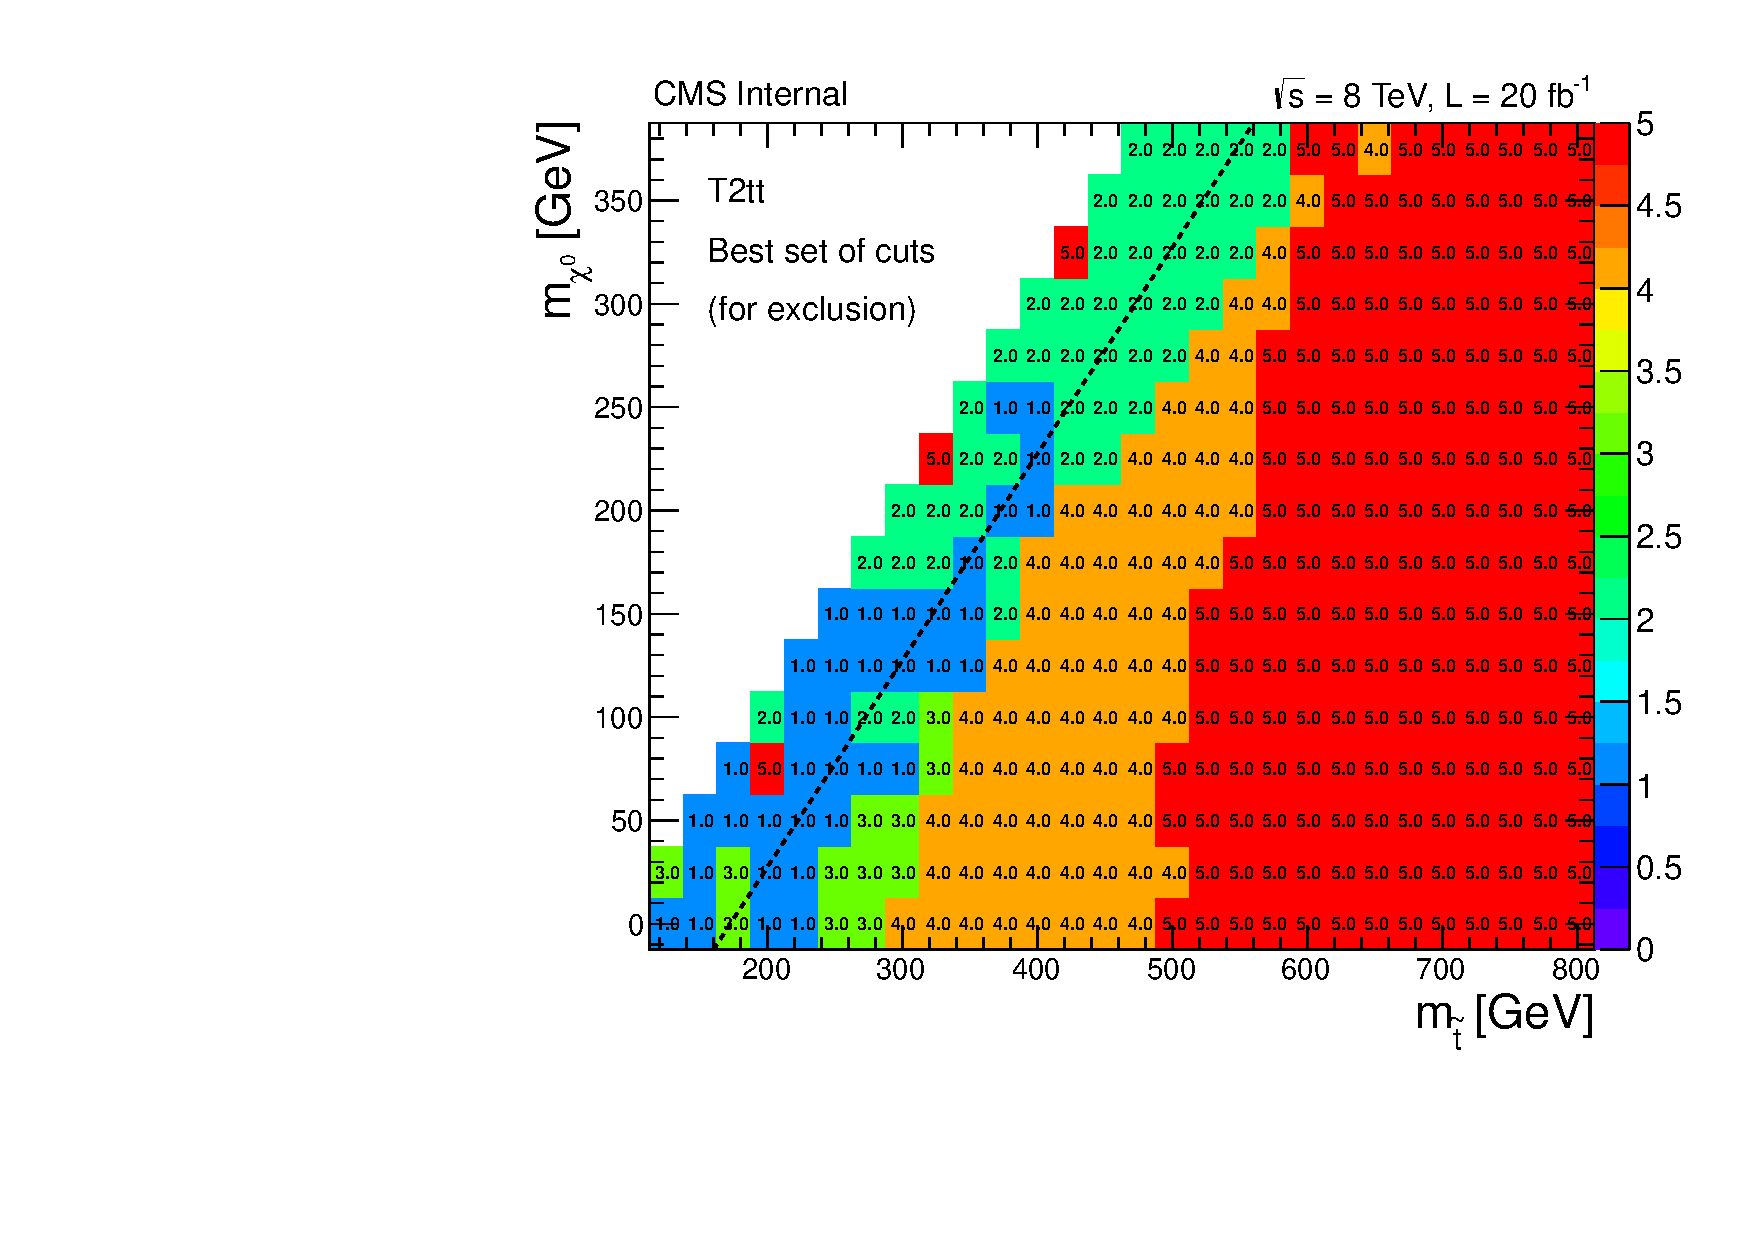
\includegraphics[width=0.39\textwidth]{cutAndCountPerformances/bestSet_T2tt}
        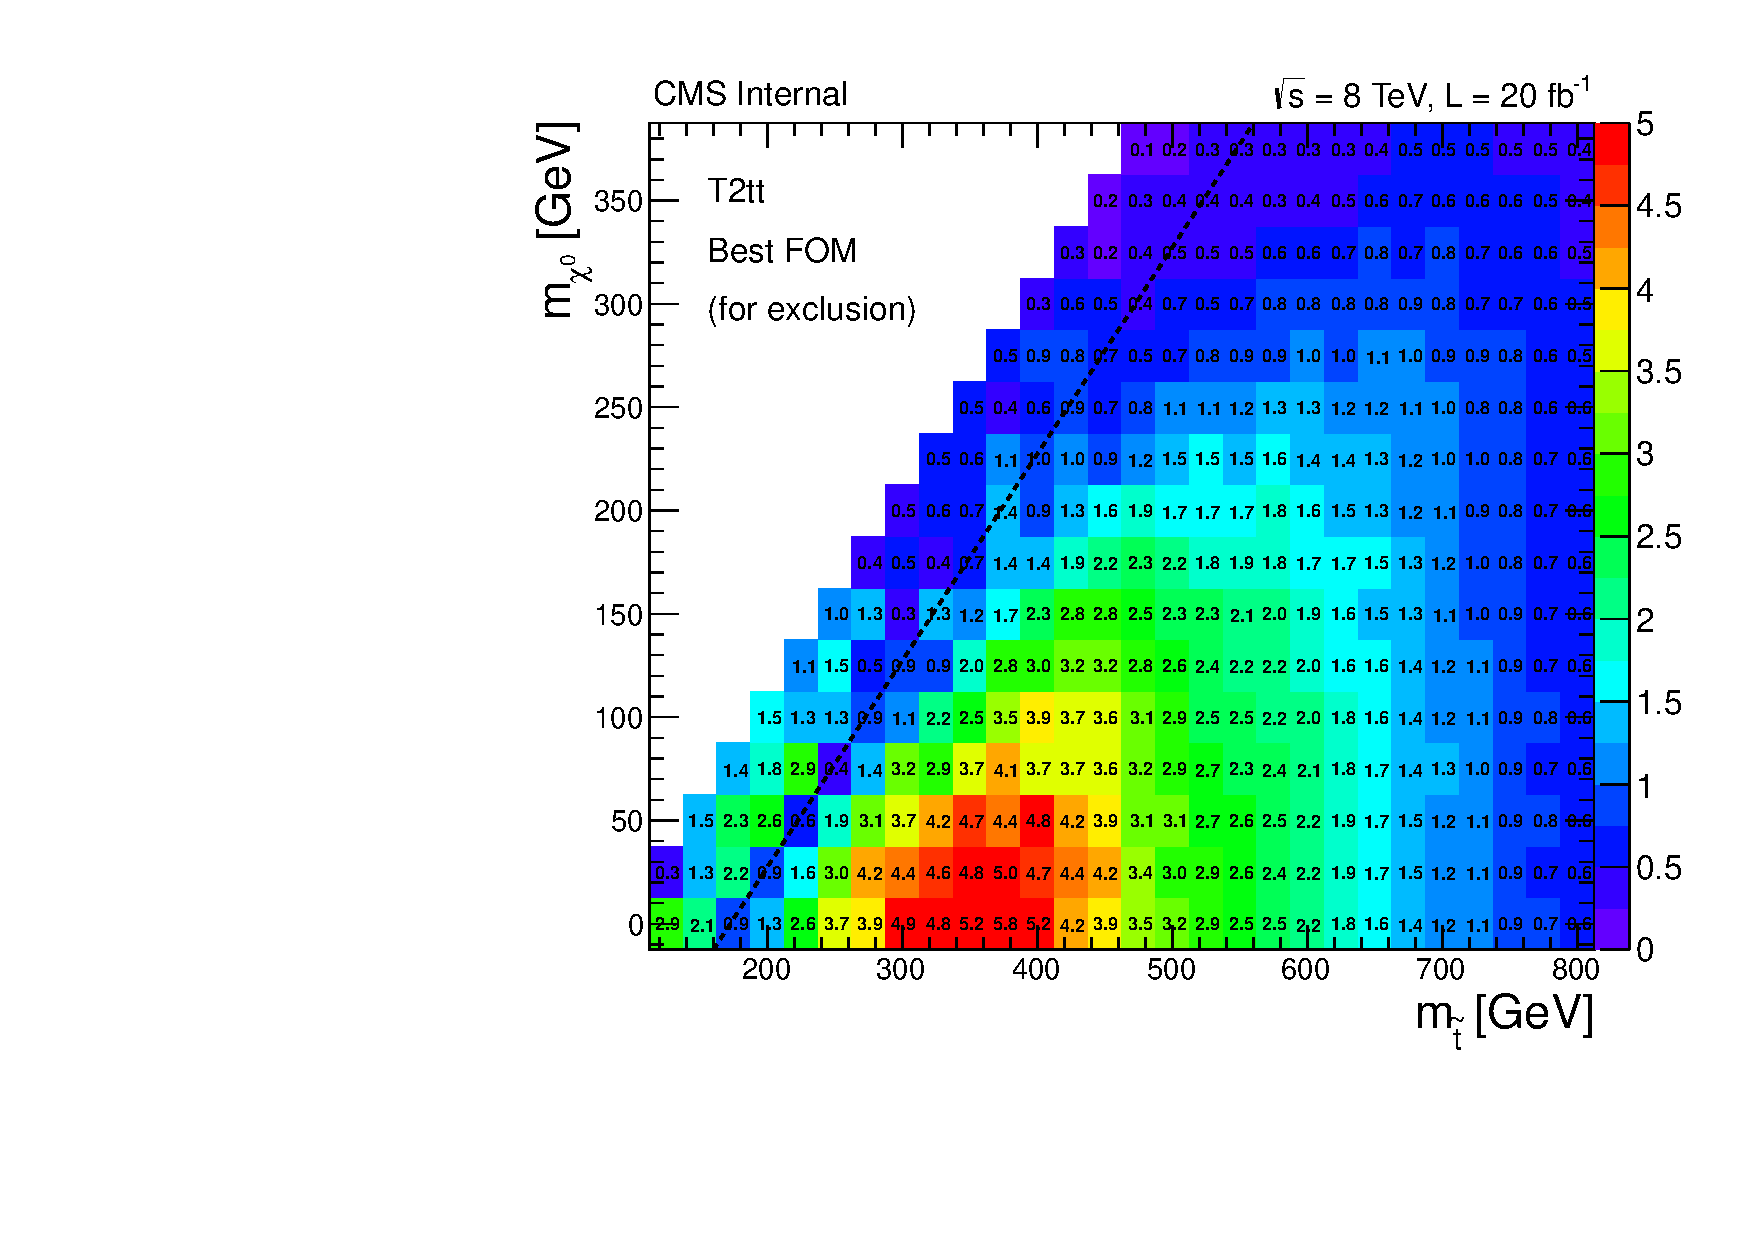
\includegraphics[width=0.39\textwidth]{cutAndCountPerformances/bestFOM_T2tt}\\
        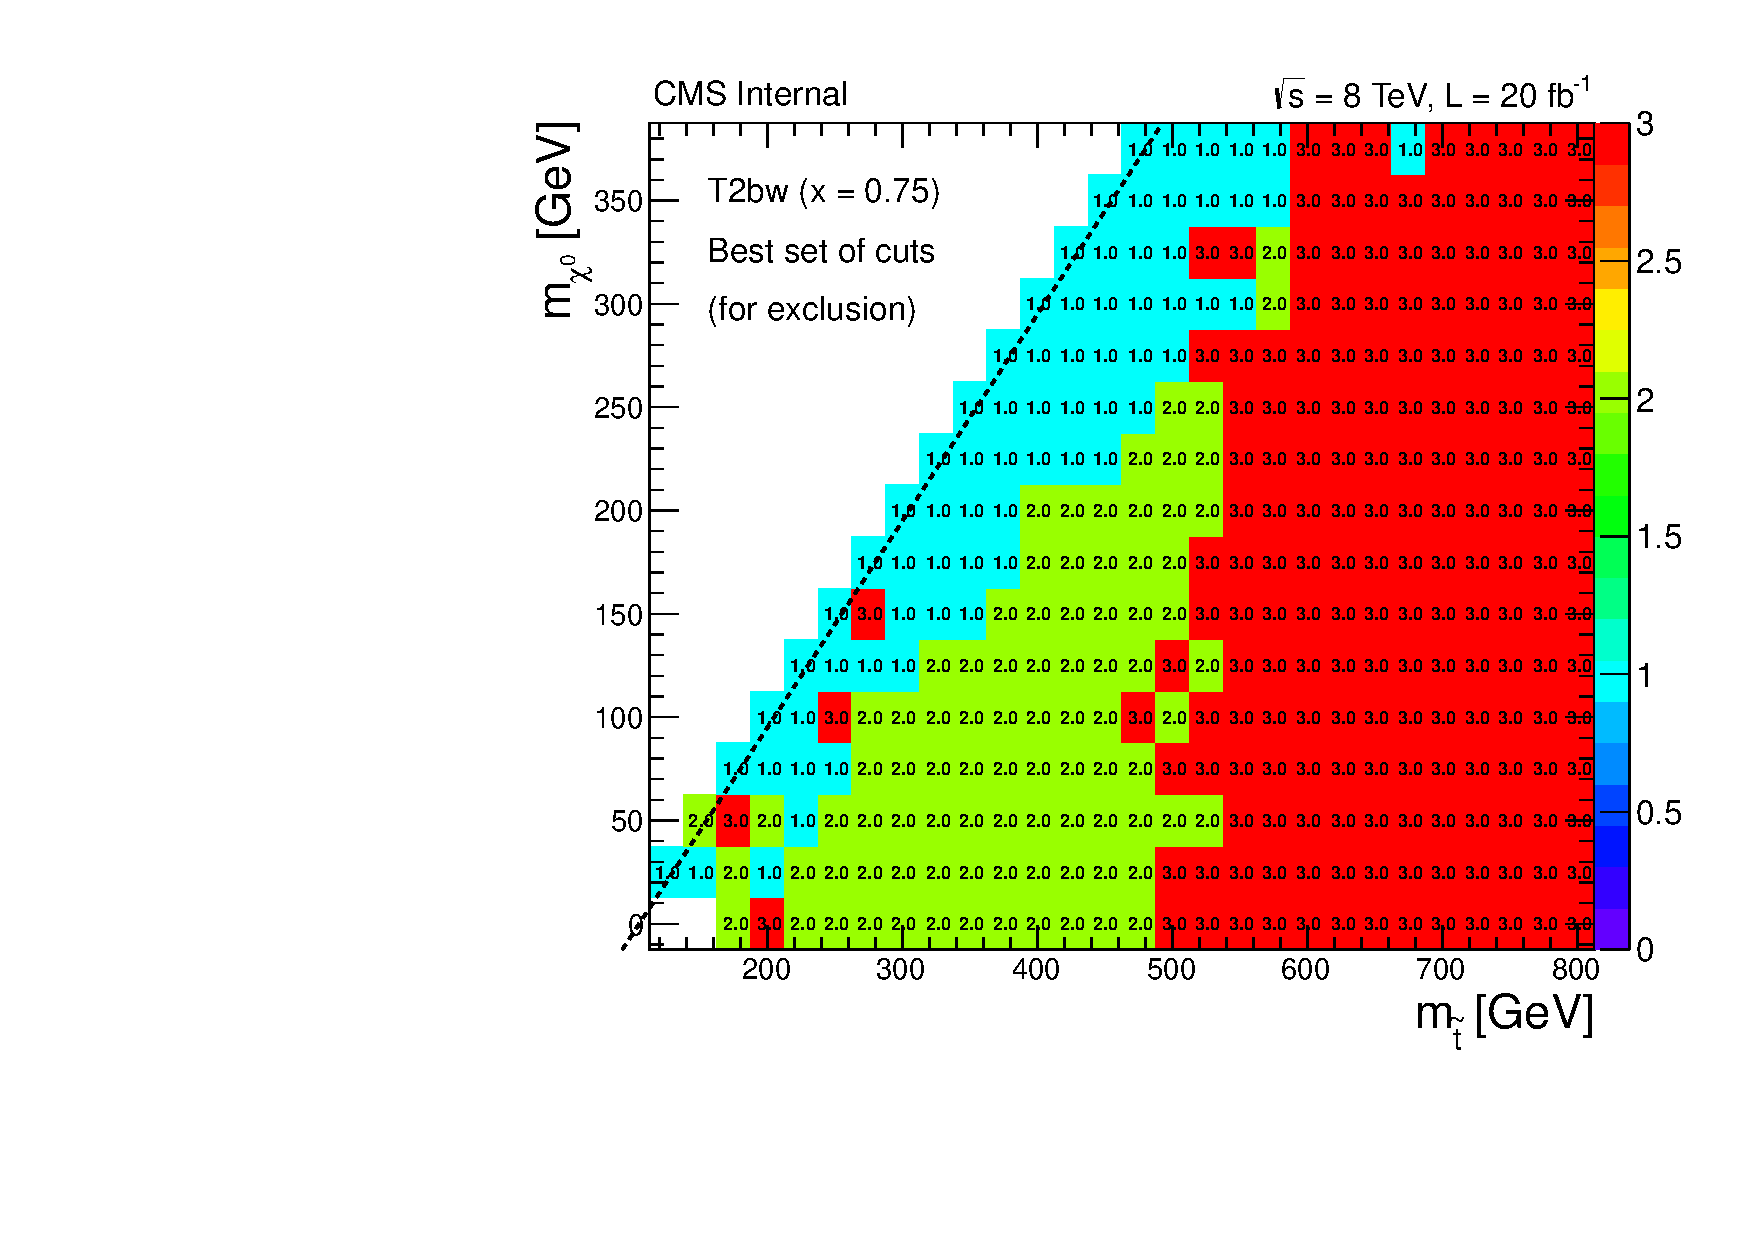
\includegraphics[width=0.39\textwidth]{cutAndCountPerformances/bestSet_T2bw075}
        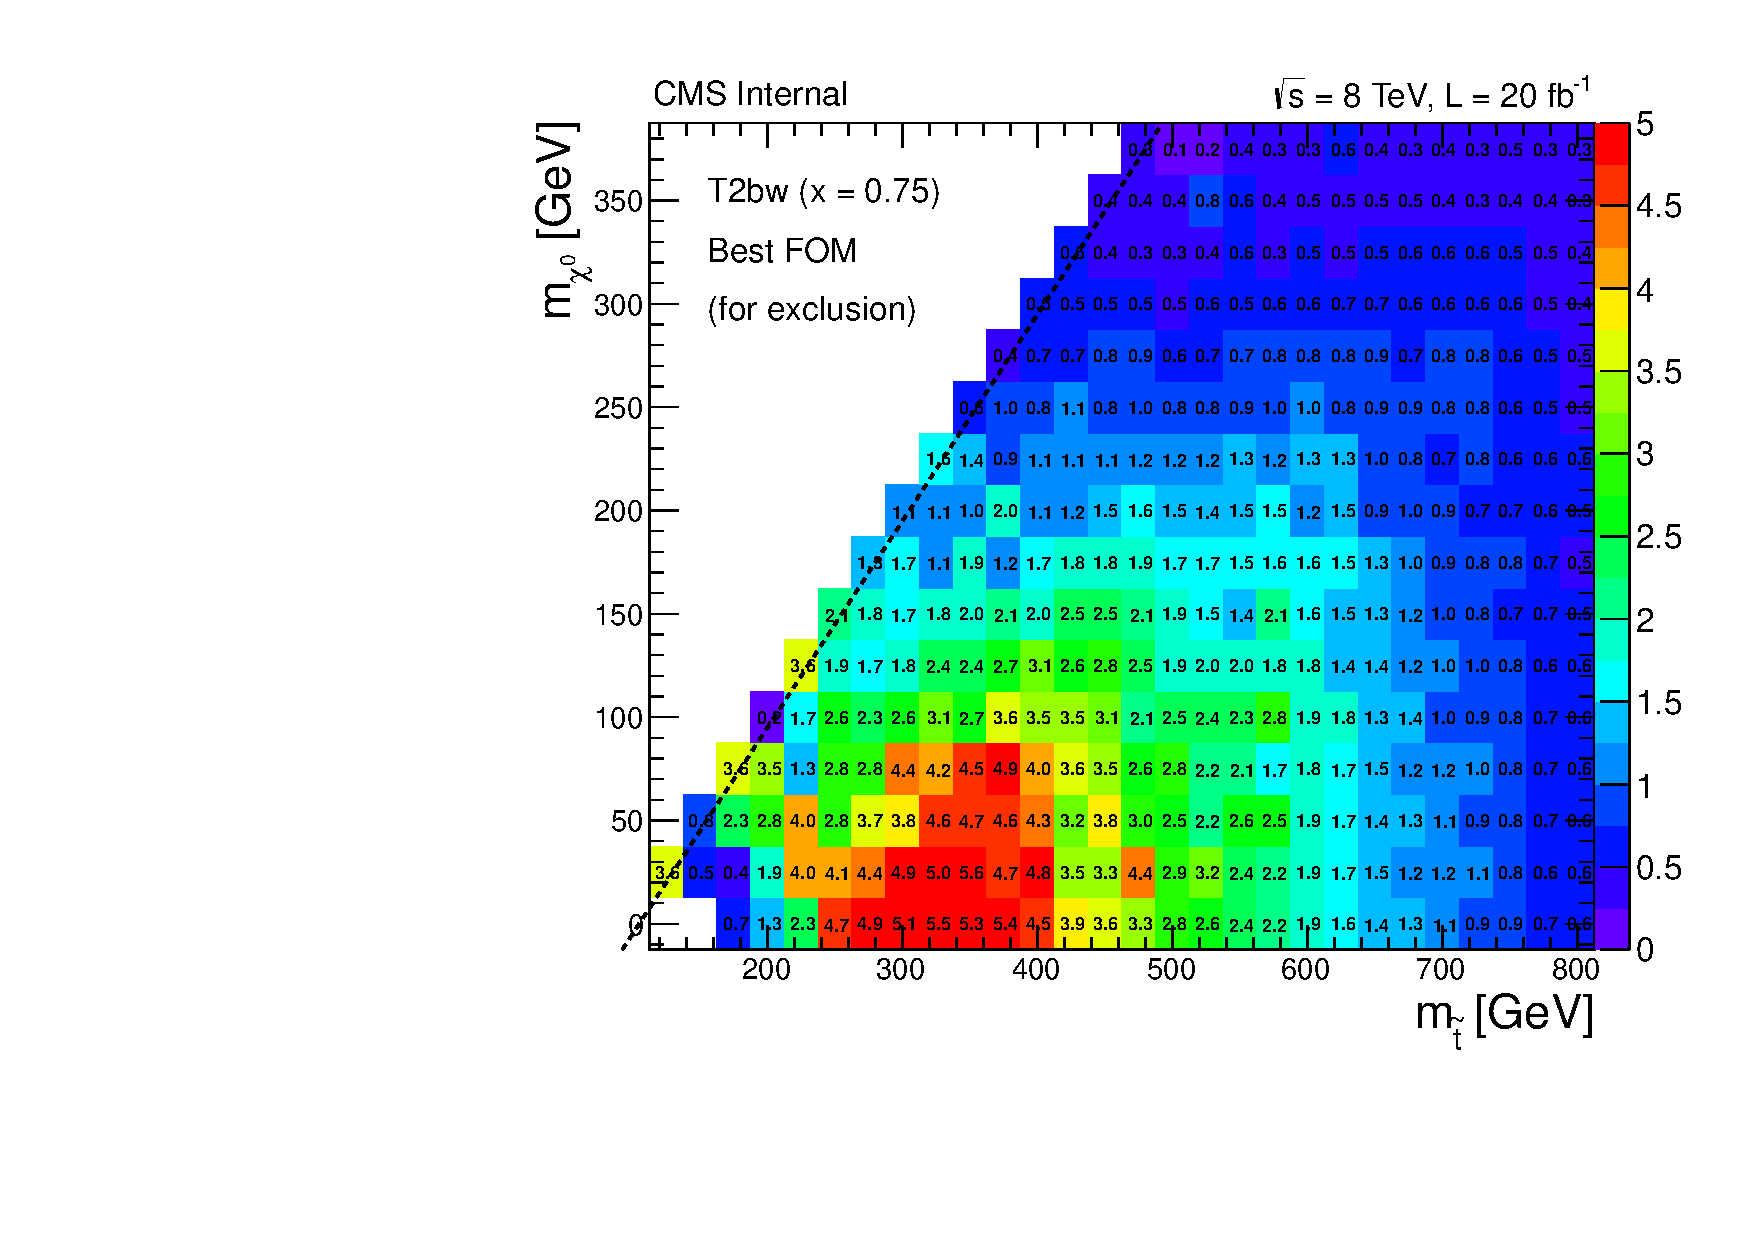
\includegraphics[width=0.39\textwidth]{cutAndCountPerformances/bestFOM_T2bw075}\\
        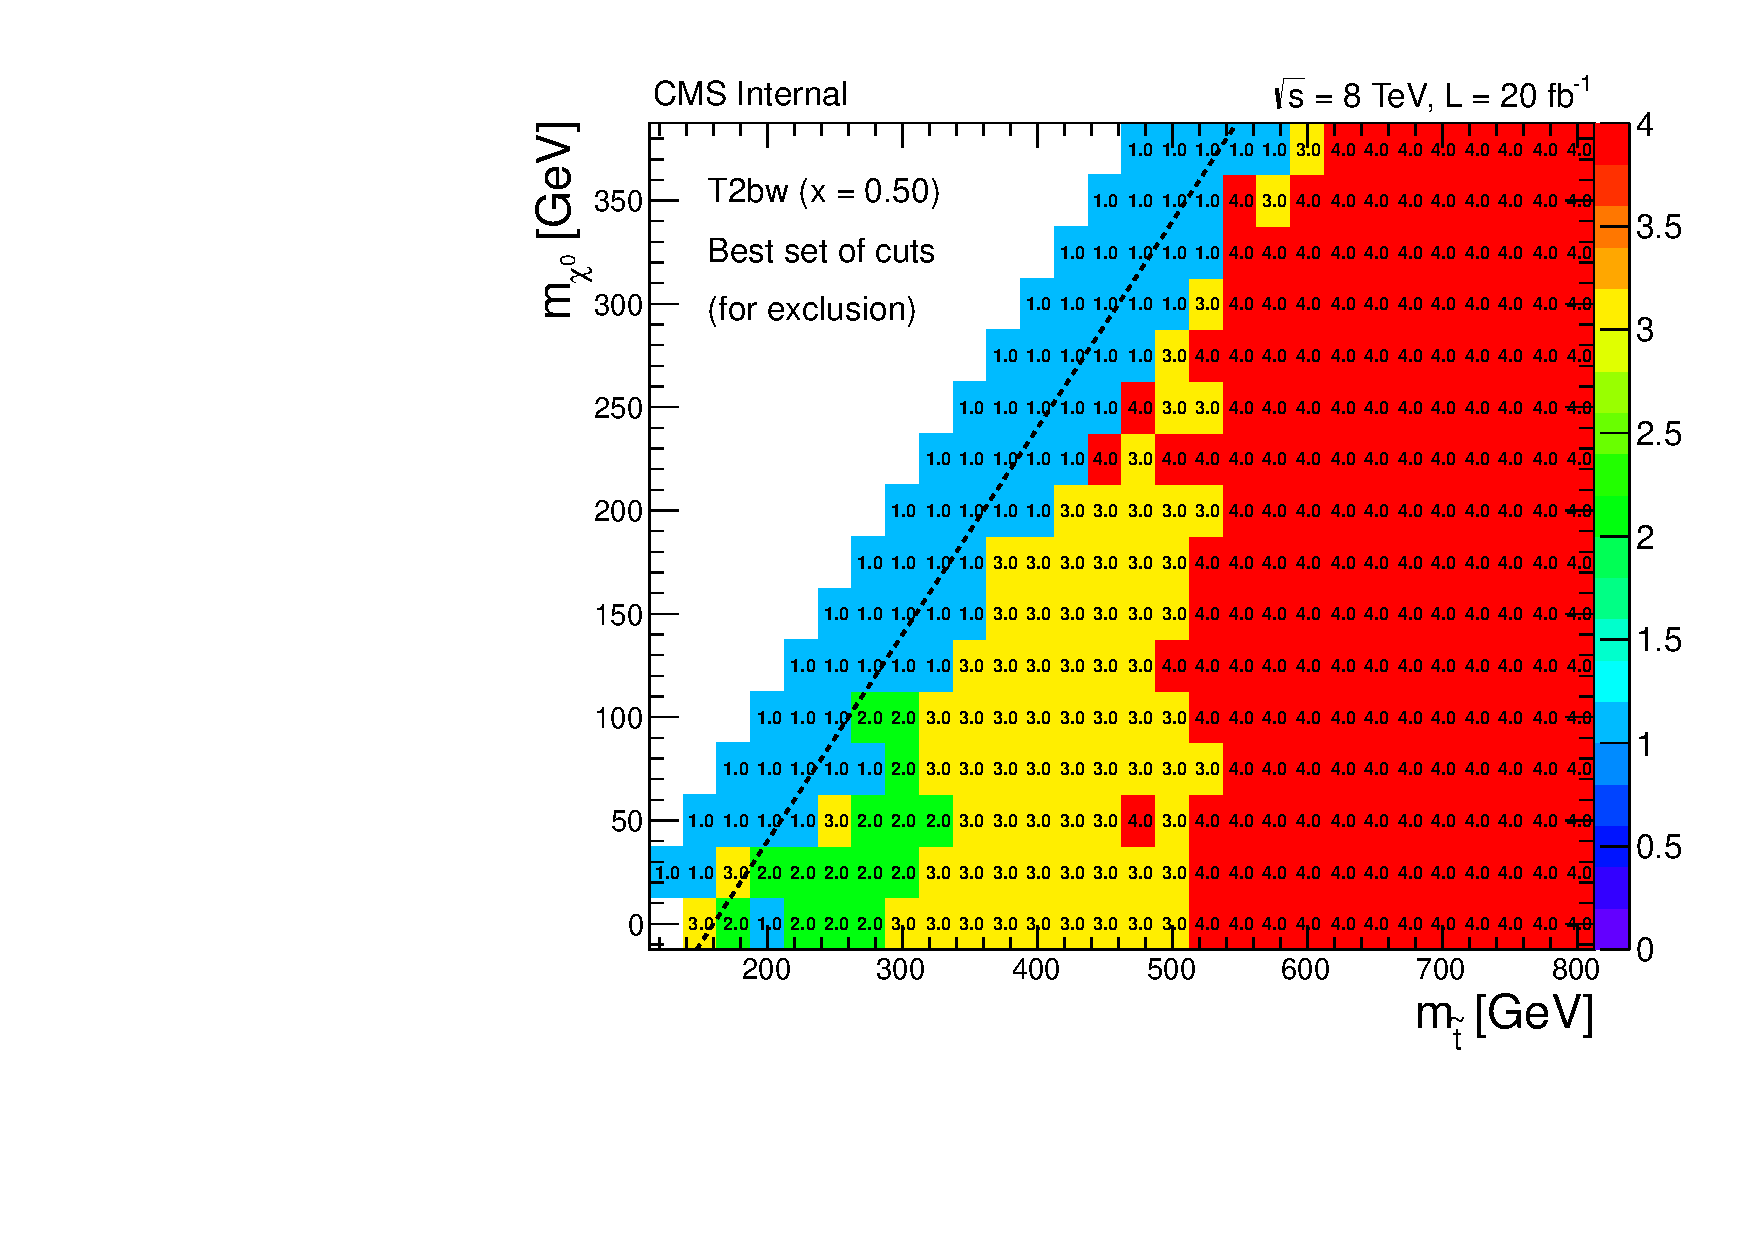
\includegraphics[width=0.39\textwidth]{cutAndCountPerformances/bestSet_T2bw050}
        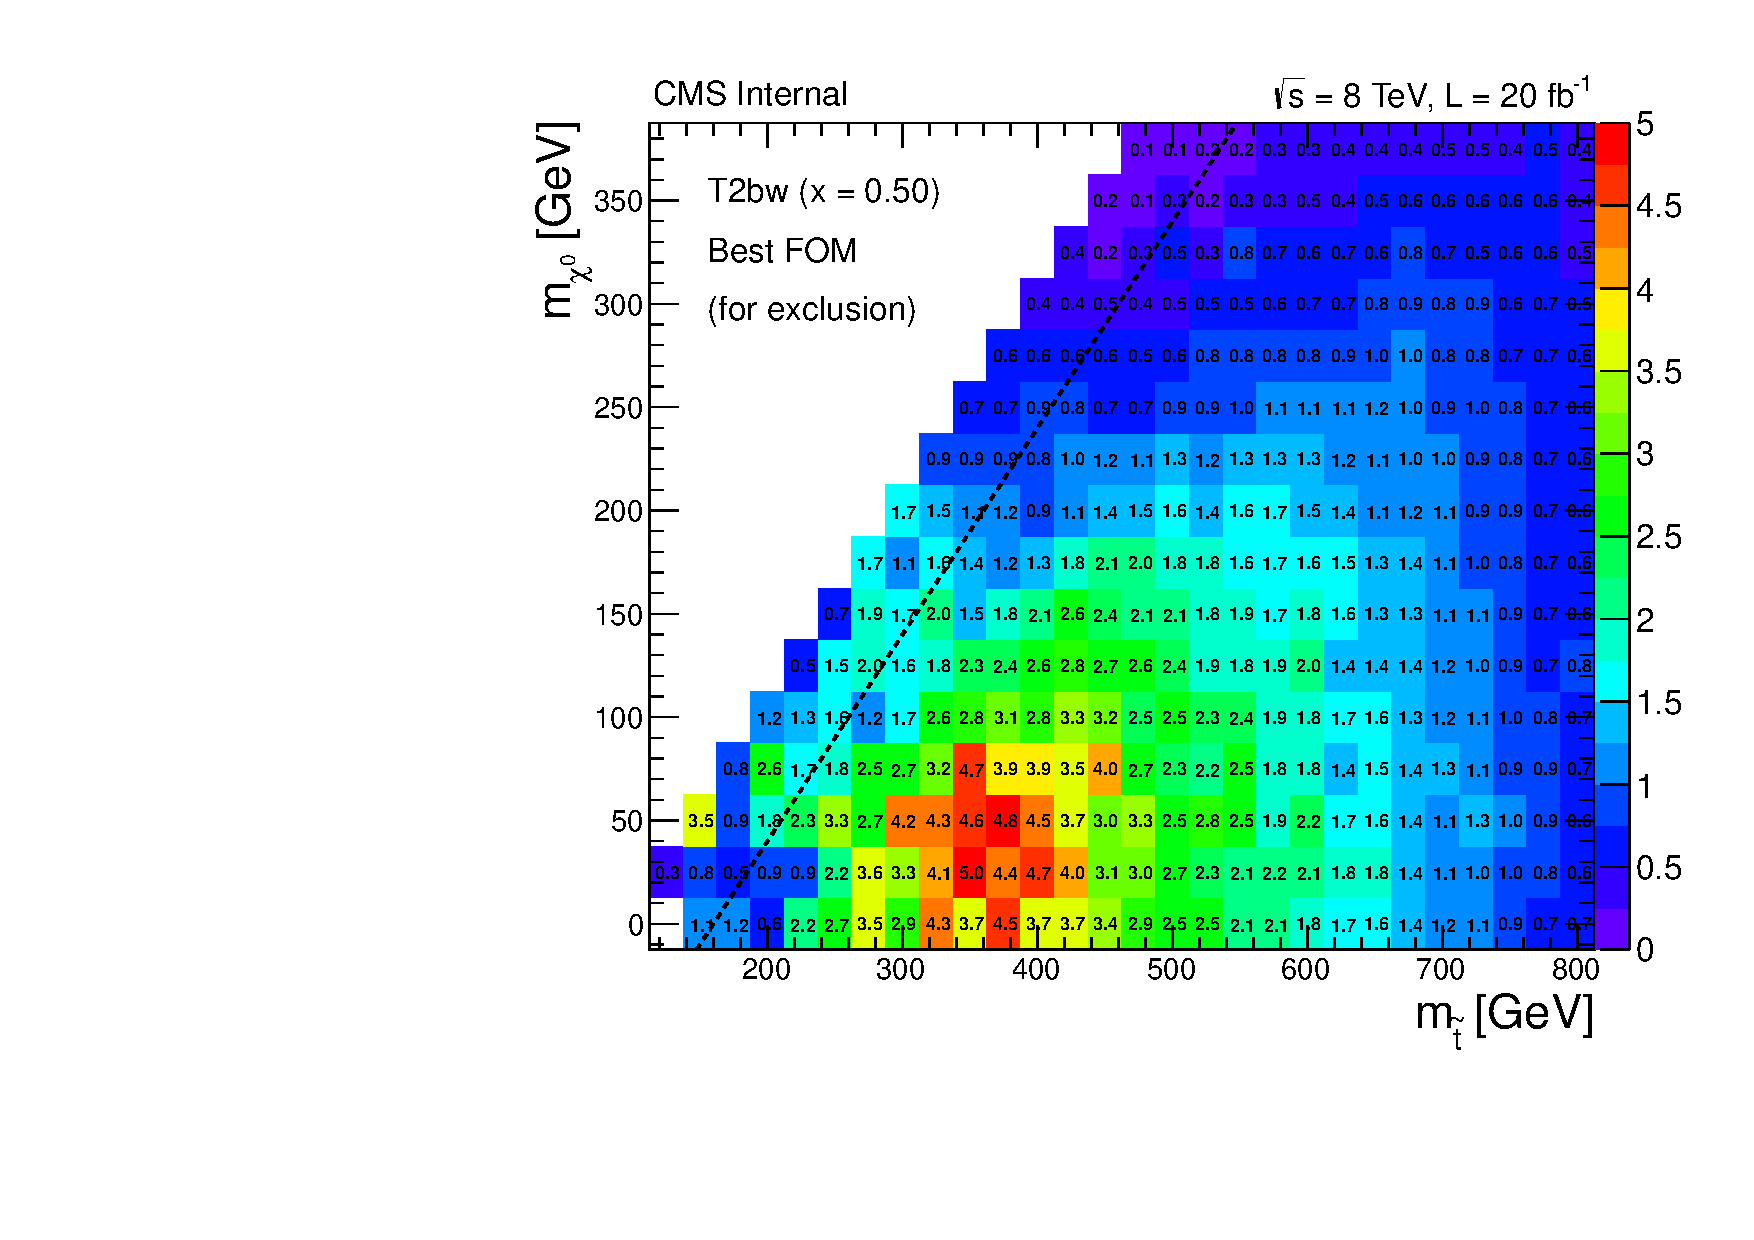
\includegraphics[width=0.39\textwidth]{cutAndCountPerformances/bestFOM_T2bw050}\\
        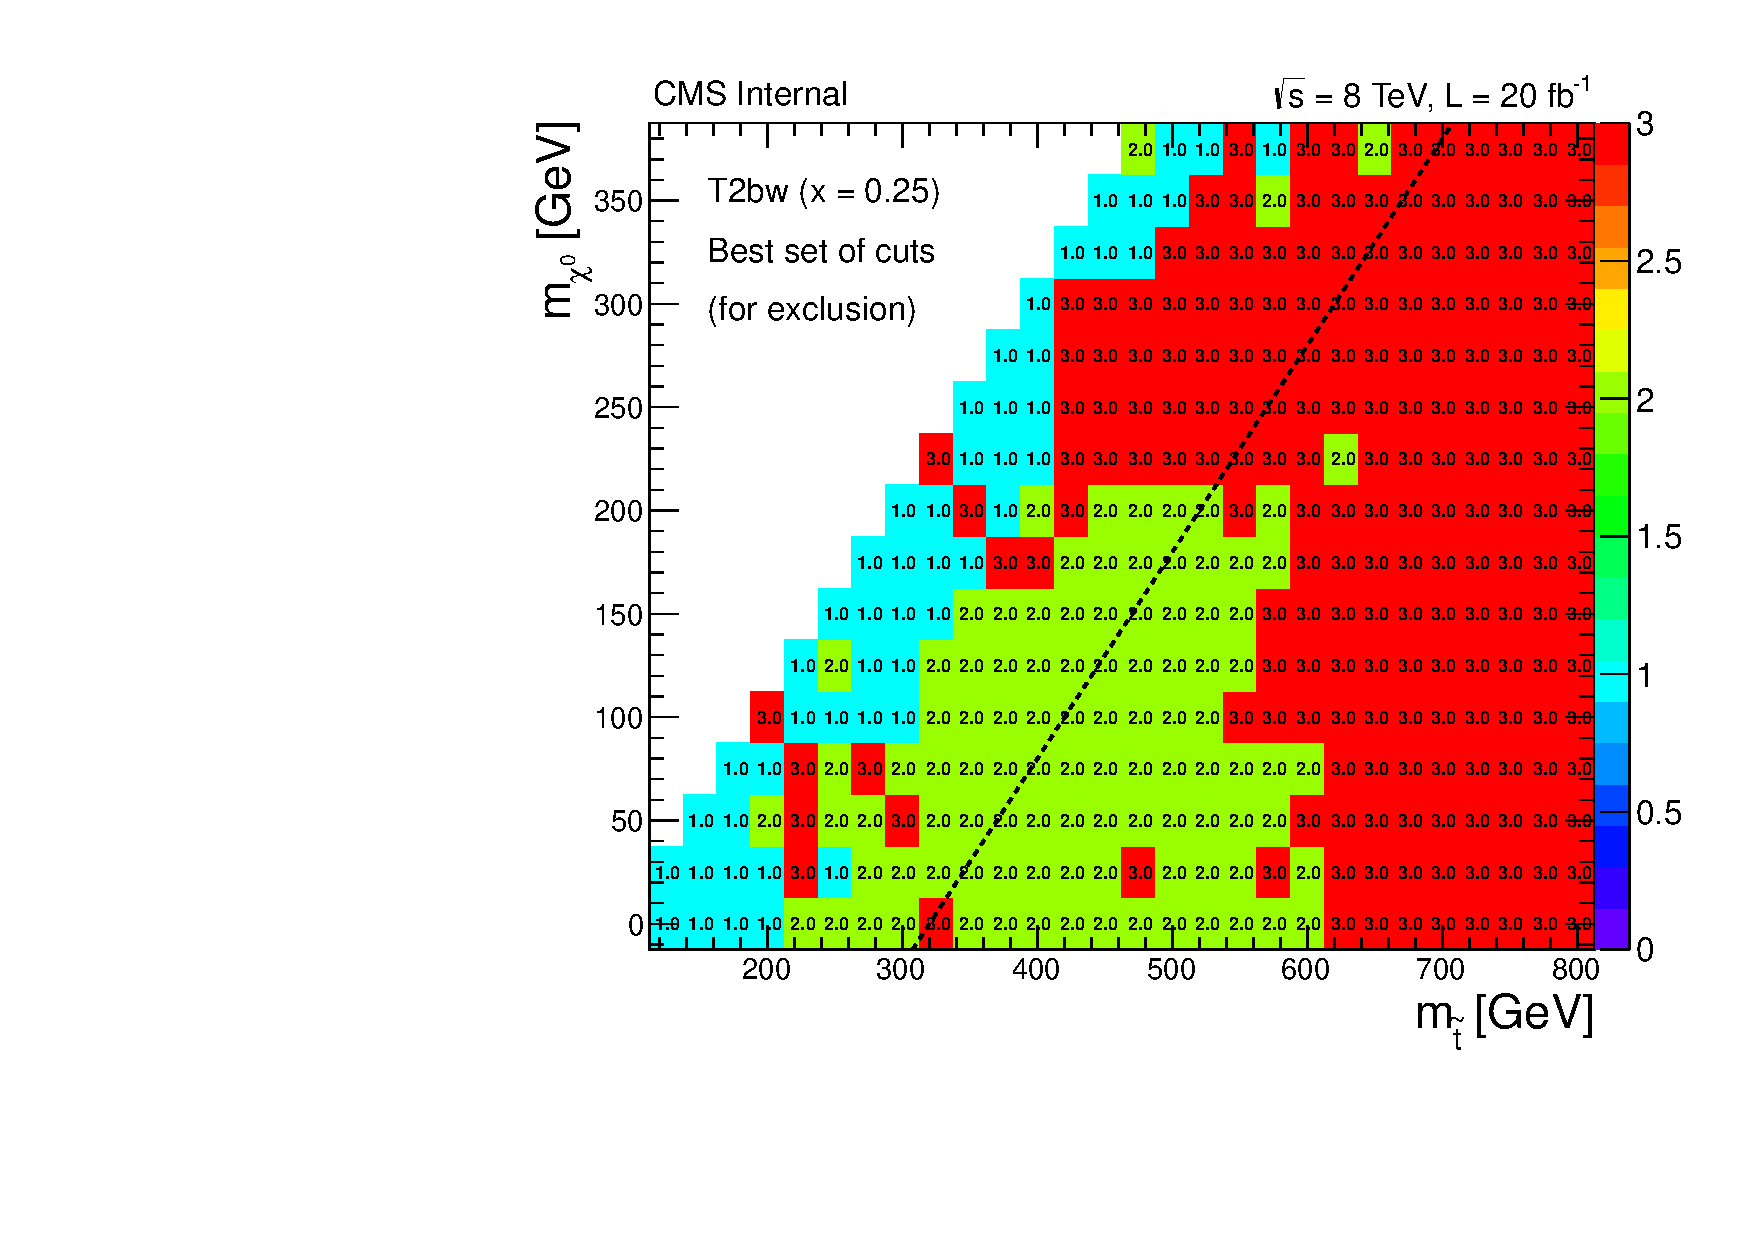
\includegraphics[width=0.39\textwidth]{cutAndCountPerformances/bestSet_T2bw025}
        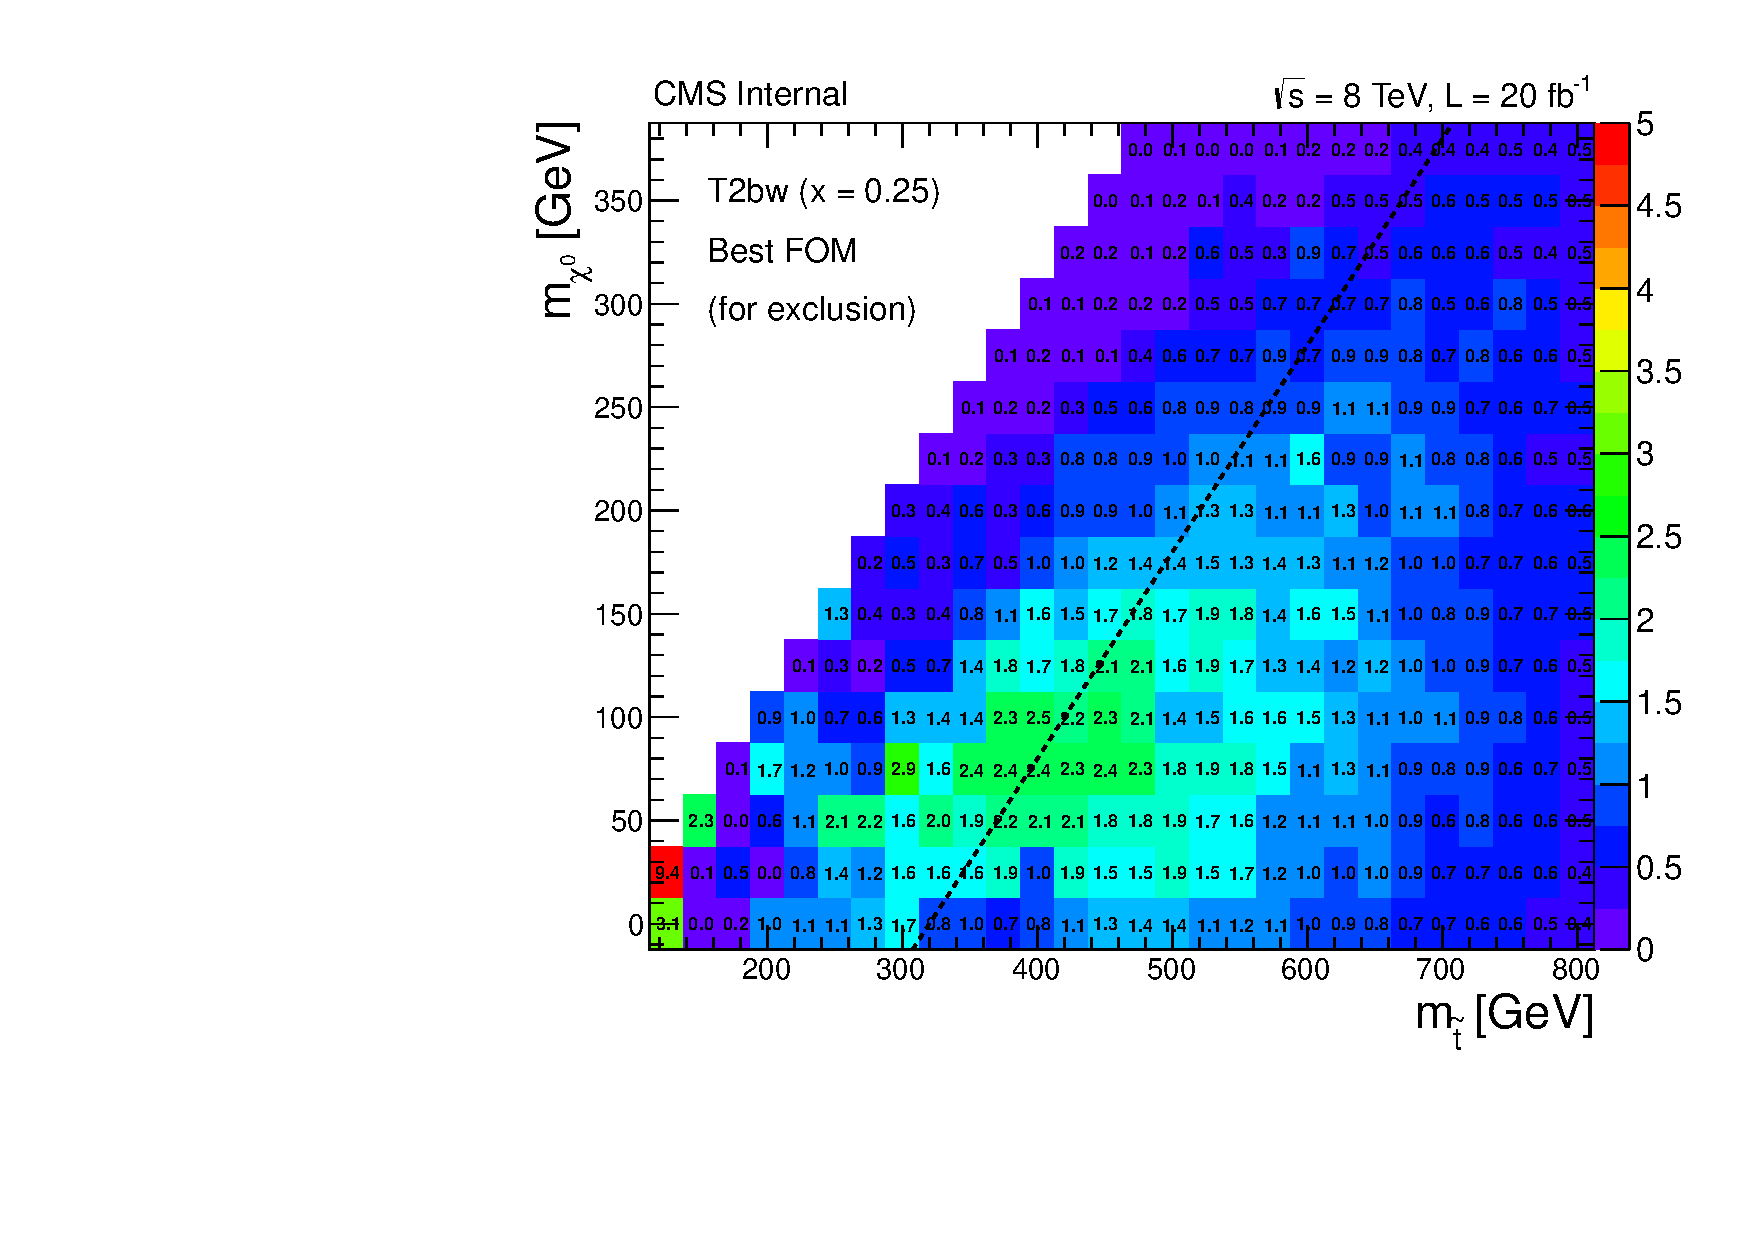
\includegraphics[width=0.39\textwidth]{cutAndCountPerformances/bestFOM_T2bw025}
        \caption{Best set of cuts (on the left) and performances in term of
        FoM$_\text{exclusion}$ (on the right) for the $\lstop \rightarrow t
        \lneutralino$ decay mode (first row) and $\lstop \rightarrow b \lchargino$
        decay mode with x = 0.75 (second row), 0.50 (third row) and 0.25 (last row).}
        \label{fig:cutAndCountPerformances}
    \end{figure}

        \subsection{BDT-based signal regions}
        %==============================================================

    For the multivariate approach, several BDT are trained on slices of $\deltam$ in the
    $(\mass{\lstop},\mass{\lneutralino})$ space against the $t\bar{t}$ background only.
    The choice of the variables is driven by an iterative method where variables are added
    to BDT and kept if the performances are overall significantly improved across different
    slices of $\deltam$. The performances of the BDTs are quantified by optimizing the cut
    on the BDT output with respect to a discovery-oriented FoM, considering all the
    backgrounds and assuming a relative systematic uncertainty of 15\%.

    The set of variables used are presented on \reftab{tab:BDTVariableUsage} as function
    of the decay mode. The definition of the training regions in the
    $(\mass{\lstop},\mass{\lneutralino})$ is then being looked at, noticing that some of
    the $\deltam$ slices can be merged together as the performances of the trainings are
    similar, essentially because the kinematic is not strongly different when moving from
    one slice to the other. The optimization of the cut on the BDT output is then performed
    by iteratively looking at the excluded cross-section after the full procedure explained
    in the following sections. The cuts are tuned manually to optimize the sensitivity
    accordingly. Here, because the cross-section regimes lead to different amount of signal
    statistics, there is sometimes a significant gain in loosening or tightening the cut
    inside a same training region.

    The final definition of the training regions is presented on \reffig{fig:BDTTrainingRegions}.
    Each number represents a different BDT training. The dashed lines represent the cases when
    one training region leads to several cuts applied to define signal regions.

    \begin{table}[h!]
        \begin{center}
            \begin{tabular}{|c|cc|}

                \hline
                Variable                            & \textsc{T2tt} & \textsc{T2tt} \\
                                                    & off-shell     & on-shell      \\
                \hline
                $\MET$                              & $\times$      & $\times$      \\
                $H_{T}^\text{ratio}$                & $\times$      & $\times$      \\
                $\pT(\text{lead. } \ell)$           & $\times$      & $\times$      \\
                $\Delta\phi(j_{1,2},\vec{\MET})$    & $\times$      & $\times$      \\
                $N_\text{jets}$                     & $\times$      & $\times$      \\
                $\pT(\text{lead. jet})$             &               & $\times$      \\
                $\Delta R( \ell, \text{lead. } b)$  &               & $\times$      \\
                hadronic top $\chi^2$               &               & $\times$      \\
                $M_{T2}^W$                          &               & $\times$      \\
                $M_{\ell b}$                        & $\times$      &               \\
                $\pT(\text{lead. } b)$              & $\times$      &               \\
                \hline
            \end{tabular}
            \begin{tabular}{|c|ccc|}

                \hline
                Variable                            & \textsc{T2bw}  & \textsc{T2bw}  & \textsc{T2bw}      \\
                                                    & $x=0.25$       & $x=0.50$       & $x=0.75$  \\
                \hline
                $\MET$                              & $\times$       & $\times$       & $\times$  \\
                $M_{T2}^W$                          & $\times$       & $\times$       & $\times$  \\
                $M_{\ell b}$                        & $\times$       & $\times$       & $\times$  \\
                $M_{3 b}$                           & $\times$       & $\times$       & $\times$  \\
                $\pT(\text{lead. } \ell)$           & $\times$       & $\times$       & $\times$  \\
                $\Delta\phi(j_{1,2},\vec{\MET})$    & $\times$       & $\times$       & $\times$  \\
                $N_\text{jets}$                     & $\times$       & $\times$       & $\times$  \\
                $\pT(\text{lead. } b)$              & $\times$       & $\times$       &           \\
                $\Delta R( \ell, \text{lead. } b)$  &                & $\times$       &           \\
                $H_{T}$                             &                &                & $\times$  \\
                $\pT(\text{lead. jet})$             &                &                & $\times$  \\
                \hline
            \end{tabular}
            \caption{List of variables considered for the training of the BDT
            as function of the decay mode. A $\times$ mark indicates that the variable
            is used in the final trainings.}
            \label{tab:BDTVariableUsage}
        \end{center}
    \end{table}

    \insertFourFigures{BDTTrainingRegions}
                      {BDT/training_T2tt}
                      {BDT/training_T2bw075}
                      {BDT/training_T2bw050}
                      {BDT/training_T2bw025}
                      {0.49}
                      {Slicing of the $(\mass{\lstop},\mass{\lneutralino})$ space
                      to define the training regions of the BDTs. Some training
                      regions are subdivided into subregions where different cuts
                      are applied on the BDT output in order to adapt the sensitivity
                      to the local signal yields.}

    \section{Background estimation \label{sec:analysis_backgroundEstimation}}
    %==============================================================

        \subsection{Overview}
        %==============================================================

    In this section, we focus on the estimation of the different background contributions.
    Four kinds of control regions are defined by inverting some of the requirements of the
    preselection and signal regions, as illustrated on \reffig{fig:backgroundEstimationOverview}.
    Each of these aims to provide a map of signal-free sectors in which to check how good is the
    modeling of the backgrounds by the Monte-Carlo and perform data-driven estimations.

        \insertFigure{backgroundEstimationOverview}{0.7}
                     {Overview of the control regions used in the background estimation method.}

    The $\MT$-peak control region is defined by looking at events satisfying $50 < \MT <
    80\GeV$ instead of the signal region $\MT$ requirement. This control region is enriched
    in $\oneLeptonTop$ and is used as a well-controlled region in which to normalize the
    $\oneLeptonTop$, $\Wjets$ and $\diLeptonTop$ as documented in \refsection{sec:MTpeakNormalization}.
    Without applying any signal region cuts, the proportion of $\oneLeptonTop$ in this
    region is about 85\%.

    The $0\, b\text{-tag}$ control region is defined by requiring no $b$-tagged jet in the
    event. This region is enriched in $\Wjets$ and $\oneLeptonTop$ and is used to control
    and correct the tail of $\MT$ for these two components as described in \refsection{sec:MTtailCorrection}.
    While it might seem counterintuitive that $\oneLeptonTop$ represents a significant
    contribution in this region, it can easily be explained by noticing that with a rough
    60\% $b$ jet efficiency of the $b$-tagging working point, there is a rough 15\% probability
    that both $b$ jets won't be tagged. Overall, without applying any signal region cuts,
    the proportion of $\Wjets$ and $\oneLeptonTop$ in this region is around 60\% and 27\%
    respectively.

    The $2\ell$ control region is designed to control the modeling of the $\diLeptonTop$
    background category, and is defined by requiring exactly two selected leptons instead
    of one, at least one jet, and lowering the $\MET$ cut to $50 \GeV$. Additionally, to
    limit the contribution from Drell-Yan, we veto events where the invariant mass of the dilepton
    system, $\mass{\ell\ell}$, is such that $\left|\mass{\ell\ell} - m_{Z}\right| < 15 \GeV$.
    As the notion of $\MT$ peak does not really exists for the $\diLeptonTop$ process,
    the full $\MT$ range is considered. Without applying any signal region cuts, the
    fraction of $\diLeptonTop$ in this region is about 93\%.

    Finally, the reversed veto control region is defined by requiring exactly one selected
    lepton and reversing the second lepton veto, effectively asking for an isolated track
    or $\tau$ candidate as defined in \refsection{sec:vetoLeptons}. This region is intended to control
    the modeling of the second lepton veto. It is being looked at in both the $\MT$ peak,
    dominated by fake second leptons in $\oneLeptonTop$, and in the $\MT$ tail dominated
    by true second leptons in $\diLeptonTop$. Without applying any signal region cuts,
    the proportion of $\oneLeptonTop$ and $\diLeptonTop$ is about 45\% for each category.

    No correction is extrapolated from the $2\ell$ and reversed veto control regions
    to the signal region as the agreement is found to be good. However, systematic uncertainties
    are derived to assess the level of confidence in the modeling of the $\diLeptonTop$ as
    detailed in \refsection{sec:background_systematics}.

    \reftab{tab:cutflowControlRegions} shows a breakdown of the background contributions
    in the different control regions at the preselection level.

\begin{table}[h!]
    \centering
\begin{tabular}{|c|cccc|}
    \hline
                     & $\MT$-peak       & $0\, b\text{-tag}$ ($M_T$ tail) & reversed veto    & 2 leptons             \\
    \hline
     $\oneLeptonTop$ & 18523 $\pm$ 55   &  1213 $\pm$ 14        &  7030 $\pm$ 34   &   41 $\pm$ 2.7  \\
     $\diLeptonTop$  &   656 $\pm$ 10   &   382 $\pm$ 8         &  7066 $\pm$ 34   & 9211 $\pm$ 39   \\
     $\Wjets$        &  1470 $\pm$ 24   &  2669 $\pm$ 33        &   331 $\pm$ 11   &  2.1 $\pm$ 0.9  \\
     rare            &  1209 $\pm$ 23   &   198 $\pm$ 7         &  1093 $\pm$ 20   &  626 $\pm$ 15   \\
    \hline
     total SM        & 21859 $\pm$ 66   &  4462 $\pm$ 38        & 15521 $\pm$ 53   & 9882 $\pm$ 42   \\
    \hline
\end{tabular}
    \caption{Breakdown of the yield of the different background categories in the four
    control regions without applying any signal region cuts. Uncertainties are statistical only.}
    \label{tab:cutflowControlRegions}
\end{table}

        \subsection{Background normalization in the $\MT$-peak region \label{sec:MTpeakNormalization}}
        %==============================================================

    The $\MT$-peak control region, defined as $50 < \MT < 80 \GeV$, is the first step of the
    background estimation method. It is used to normalize the $\oneLeptonTop$, $\Wjets$ and
    $\diLeptonTop$ components while the rare component is taken directly from Monte-Carlo.
    It is important to note that this normalization is done for each signal region individually,
    effectively allowing to absorb disagreements caused by cuts on variables that may not
    be perfectly modeled, as well as uncertainties on the jet energy scale, the trigger efficiency,
    the lepton identification efficiency and the luminosity.

    To separate the effect of the second lepton veto, the  normalization is done in two
    steps: first, a scale factor $\SFpre$ is computed before the application of the
    second lepton veto, subtracting the rare component:

    \begin{equation}
        \SFpre
        \definedAs
        \left(
            \frac{N(\text{data}) - N(\text{rare})}
                 {N(\oneLeptonTop) + N(\Wjets) + N(\diLeptonTop)}
        \right).
        \label{eq:SFpreDefinition}
    \end{equation}

    $\SFpre$ is used to normalize only the $\diLeptonTop$ component. Another scale factor,
    $\SFpost$ is used after application of the second lepton veto, subtracting the rare
    and the corrected $\diLeptonTop$ component:

    \begin{equation}
        \SFpost
        \definedAs
        \left(
            \frac{N(\text{data}) - N(\text{rare}) - \SFpre \times N(\diLeptonTop)}
                 {N(\oneLeptonTop) + N(\Wjets)}
        \right).
        \label{eq:SFpostDefinition}
    \end{equation}

     When applying no signal region cuts, $\SFpre$ and $\SFpost$ are equal to
     $(1.06 \pm 0.01)$ and $(1.05 \pm 0.01)$ respectively. This values, while not
     being compatible with 1, can be interpreted as a relatively small disagreement
     which is attributed to the misknowledge of the previously listed effects. Across the
     different cut-based signal regions, these scale factors range from $0.8$ to $1.4$,
     sometimes only compatible with unity at 3 standard deviations. The magnitude of this
     effect is attributed to bad modeling of the far tail of some variables in the
     Monte-Carlo.

        \subsection{$\MT$-tail correction in the $0\, b\text{-tag}$ region \label{sec:MTtailCorrection}}
        %==============================================================

    The $0\, b\text{-tag}$ control region allows to control the tail of $\MT$ for the $\Wjets$ and
    $\oneLeptonTop$ components. Before looking at the tail, however, we start by normalizing
    the background in the $\MT$ peak of this control region, in a similar fashion to what
    is done in \refsection{sec:MTpeakNormalization}. This is done by introducing $\SFnobtag$,
    used to normalize the $\Wjets$ and $\oneLeptonTop$ contributions:

    \begin{equation}
        \SFnobtag
        \definedAs
        \left(
            \frac{N(\text{data}) - N(\text{rare}) - N(\diLeptonTop)}
                 {N(\oneLeptonTop) + N(\Wjets)}
        \right)
        \label{eq:SF0btagDefinition}
    \end{equation}

    Without applying any signal cuts, $\SFnobtag$ is found to be $(0.99 \pm 0.01)$.
    After normalization to the peak, a clear disagreement in the tail of $\MT$ is observed
    for $\MT > 100 \GeV$ between the data and Monte-Carlo, as shown on
    \reffig{fig:templateFit/MT_notCorrected}. This disagreement is a known feature
    also observed by several other analyses \cite{WjetsDifferentialCrossSection, LeptonicMonotop,
    B2GttMET}. This is an important point of the analysis as
    it means that the Monte-Carlo needs to be corrected to have a reliable prediction of
    the $\oneLeptonTop$ and $\Wjets$ in the $\MT$ tail.

    \insertFigure{templateFit/MT_notCorrected}{0.55}
                 {Data/MC comparison on the full $M_T$ distribution in the $0\, b\text{-tag}$ control
                 region at preselection level, after propagation of $\SFnobtag$. A clear
                 discrepancy is visible for $\MT > 100 \GeV$.}

    One can investigate the origin of the disagreement by first getting a better idea from
    the Monte-Carlo simulation of what is causing $\oneLeptonTop$ and $\Wjets$ events
    to reach the tail of $\MT$. The resolution of $\MT$ is strongly related to both the
    resolution in energy of $\vec{\MET}$, and its $\Delta\phi$ with the lepton. The relative
    resolutions of $\MET$ and $\Delta \phi$ are investigated in the Monte-Carlo, defined
    as the ratio of the reconstructed quantity versus the generated quantity, constructed
    from the generated prompt neutrinos in the event. \reffig{fig:MTtailResolution} shows
    the distributions of the relative resolutions of $\MET$ and $\Delta \phi$ as function
    of $\MT$ for the $\oneLeptonTop$ background and their mean values for each background.

    \insertFourFigures{MTtailResolution}
                      {MTtailResolution/MTvsMETReso}
                      {MTtailResolution/MTvsDeltaPhiReso}
                      {MTtailResolution/MTvsMeanMETReso}
                      {MTtailResolution/MTvsMeanDeltaPhiReso}
                      {0.45}
                      {$\MET$ and $\Delta \phi$ relative resolutions as function of $\MT$,
                      using the generated $\MET$ from neutrinos coming from a $W$ boson, on top
                      showing the full 2 dimensional distribution and on bottom showing
                      the evolution of the mean resolution for each background. Error
                      bars correspond to the uncertainties on the mean estimation.}

    The results of this quick investigation tends to point out that the $\MT$ tail for
    the $\oneLeptonTop$, $\Wjets$ and rare backgrounds originates more from the
    misreconstruction of the magnitude of the $\MET$ rather than its direction. Small
    features are however observed in the $\Delta \phi$ spectra which can originate from
    other sources of genuine $\MET$ in the event such as neutrinos inside $b$ jets.

    So far, the method used to correct the discrepancy is to compute ad-hoc scale factors
    using a template fit that estimate separately the contribution of $\oneLeptonTop$ and
    $\Wjets$ backgrounds from the data. To do this, we use $\MlbPrime$ which was found to have a good
    discriminating power between the two process categories and being well described in
    the peak of $\MT$, as shown on \reffig{fig:MlbPrimeForTemplateFit}.

    \insertFourFigures{MlbPrimeForTemplateFit}
                      {templateFit/Mlb_0b_peak}
                      {templateFit/Mlb_0b_tail}
                      {templateFit/preselection_Mlb_noFit}
                      {templateFit/preselection_Mlb_withFit}
                      {0.45}
                      {Distribution of $\MlbPrime$ in the $0\, b\text{-tag}$ control region,
                      data/MC comparison in the $M_T$ peak (top left), superimposed and
                      normalized $\oneLeptonTop$ and $\Wjets$ components in the $M_T$ tail
                      (top right), data/MC comparison in the $M_T$ tail before correction
                      of the Monte-Carlo (bottom left) and after correction (bottom right).
                      On the bottom right, the uncertainties on the scale factors are
                      propagated in the ratio.}

    The method is implemented using the \textsc{RooFit} toolbox \cite{RooFit} with the Minuit2
    implementation of the \textsc{Migrad} minimizer algorithm. The normalization
    of the $\oneLeptonTop$ and $\Wjets$ components are free parameters translated in term
    of scale factors, $SF_{\oneLeptonTop}$ and $SF_{\Wjets}$, while the normalization of
    the $\diLeptonTop$ and rare components are taken from the Monte-Carlo and constrained
    with a 20\% uncertainty during the fit process. To validate the method, a closure test
    is performed by generating toy data from the Monte-Carlo where arbitrary scale factors
    were injected. The estimated scale factors are then compared to the input scale factors.
    A very good linearity is found for scale factors varying from 0.10 to 3.

    The fit is
    performed both in the $\MT$ peak and tail regions and we extract $SFR = SF^{\text{tail}}
    / SF^{\text{peak}}$ for both processes, representing the discrepancy in the tail
    independently from the peak normalization. Different sources of systematic uncertainty
    are considered: the jet energy scale, the normalization of the rare and $\diLeptonTop$ background, the
    Monte-Carlo statistics, the choice of the minimizer algorithm, the choice of the
    initial fit conditions, the generator setup for $t\bar{t}$ (using \textsc{Powheg} or
    \textsc{MadGraph}, varying the matching parameters, RGE scale, top mass, applying or
    not the top $\pT$ reweighting). The most important sources are the Monte-Carlo statistics
    (leading to 11\% of relative uncertainty on SFR), the generator scale (9\%) and the jet
    energy scale. A conservative 20\% is used as relative systematic uncertainty.

    Without applying any signal region cuts, $\SFRoneLeptonTop$ and $\SFRWjets$ are found
    to be $(1.04 \pm 0.16 (\text{stat.}) \pm 0.21 (\text{syst.}))$ and $(1.33 \pm 0.10
    (\text{stat.}) \pm 0.27 (\text{syst.}) )$ respectively. The plot on bottom right
    of \reffig{fig:MlbPrimeForTemplateFit}
    illustrates the impact on the $\MlbPrime$ data/MC comparison after propagating the scale
    factors.

    For the cut-based signal regions, we
    use the scale factors derived from a single $\MT$ cut associated to the signal region
    as shown on \reffig{fig:templateFit/CnC_MTcuts}. It is found that the $\SFRoneLeptonTop$
    increases as function of the $\MT$ cut applied while $\SFRWjets$ is relatively constant
    around 1.33. This is a clear indication that a separate treatment is necessary between
    these two background categories. To cover possible correlation between the $SFR$ and
    $\MET$ or $\MET/\sqrt{H_T}$, the computation of the scale factors is also studied for
    single $\MET$ or $\MET/\sqrt{H_T}$ cuts, as shown on \reffig{fig:templateFitCnCResultsMET}.
    The final scale factors applied for a given signal region are the $SFR$ derived for the
    single $\MT$ cut associated to that signal region, to which we quadratically add the
    uncertainty extracted from the $SFR$ computed with the single $\MET$ or $\MET/\sqrt{H_T}$
    cut associated to that signal region.

    For the BDT signal regions, to be as close as possible to the kinematic of the BDT tails,
    we choose cuts on each BDT outputs such as at least 25\% of the background is still
    selected and apply the template fit method in that region. Two common scale factors
    to be applied to each BDT are then computed by averaging across all the trainings.
    The values found are $\SFRoneLeptonTop = (1.38 \pm 0.61)$ and $\SFRWjets = (1.21 \pm 0.36)$.

        \insertFigure{templateFit/CnC_MTcuts}
                     {0.6}
                     {Template fit results for individual cuts on $\MT$ after
                     preselection. The uncertainties shown are statistical only.}

        \insertTwoFigures{templateFitCnCResultsMET}
                         {templateFit/CnC_METcuts}
                         {templateFit/CnC_METoverSqrtHTcuts}
                         {0.45}
                         {Template fit results for individual cuts on $\MET$ (left)
                         and $\MET/\sqrt{H_T}$ (right) after preselection + $\MT > 100\GeV$.
                         The uncertainties shown are statistical only.}

        \subsection{Control of the $\diLeptonTop$ component and second lepton veto \label{sec:analysis_controlDileptonTop}}
        %==============================================================

        The 2-lepton and reversed veto control regions allow to check for the good modeling
        of the $\diLeptonTop$ background and the second lepton veto definition. In the
        2 lepton control region, $\MT$ is defined using the leading lepton and ignoring
        the second one. The $\MT$-peak of the reversed veto control region is dominated by
        $\oneLeptonTop$ where a fake second lepton was reconstructed while the $\MT$-tail
        is dominated by $\diLeptonTop$ with a true second lepton. As for the $\MT$-peak
        normalization, we introduce scale factors to normalize the backgrounds in the peak
        of $\MT$ and then quantify the agreement in the tail.

        In the reversed veto region, we define $\SFveto$ in a similar fashion as $\SFpost$,
        to control the fake-dominated region, and $\SFvetoTail$ to control region dominated
        by true second lepton, after propagation of all the relevant scale factors including
        $\SFRoneLeptonTop$ and $\SFRWjets$.
        Without applying any signal region cuts, we find $\SFveto = (1.18 \pm 0.03)$ and
        $\SFvetoTail = (1.07 \pm 0.02)$. The relatively large value of $\SFveto$ is
        interpreted as a mismodeling of the fake rate of the lepton veto by the Monte-Carlo.
        Despite being not compatible with unity, this SF is not used to compute the prediction
        in the signal region because its effect is already included in $\SFpost$. The
        value of $\SFvetoTail$ also manifests a discrepancy in the lepton veto selection
        efficiency. Despite the fact that this scale factor is not propagated to the
        signal region, a systematic is later introduced to cover this effect.

        In the 2 leptons control region, we define $\SFtwoLep$ and $\SFtwoLepTail$ to
        control respectively the whole $\MT$ distribution and the tail of it.
        Without applying any signal region cuts, we find $\SFtwoLep = (0.96 \pm 0.01)$
        and $\SFtwoLepTail = (1.01 \pm 0.02)$ showing therefore a good modeling of $\MT$
        for this background.

        \reffig{fig:preselMT2leptonAndLepPlusVeto} presents the full $\MT$ distributions
        for the reversed veto and two leptons control regions where a good agreement is
        found after propagating the scale factors $\SFpre$, $\SFveto$, $\SFRoneLeptonTop$
        and $\SFRWjets$ where it is relevant.
        Another important check in the 2 leptons control region is the jet multiplicity
        modeling of $\diLeptonTop$ as the four jets requirement corresponds to two
        additional jets coming from radiations or pile-up for this background.
        \reffig{fig:controlPlots/2leptons/nJets} presents the distribution of the number
        of selected jets after application of $\MT>100$, which is found in good agreement.


        \begin{figure}[h!]
            \centering
            \includegraphics[width=0.45\textwidth]{controlPlots/reversedVeto_noMTCut/MT}
            \includegraphics[width=0.45\textwidth]{controlPlots/2leptons_noMTCut/MT}
            \caption{Full $\MT$ distributions for the reversed veto control region (on the left) and two leptons control region (on the right). On the left, $\SFpre$, $\SFveto$, $\SFRoneLeptonTop$ and $\SFRWjets$ are propagated. On the right, no scale factors is applied.}
                    \label{fig:preselMT2leptonAndLepPlusVeto}
        \end{figure}

        \insertFigure{controlPlots/2leptons/nJets}
                     {0.5}
                     {Distribution of the number of selected jets in the two leptons control
                     region after applying $\MT > 100$. No scale factor is applied on the
                     distribution.}

        \subsection{Control of variables at preselection level}
        %==============================================================

        The modeling of each variables is validated in each control region without applying
        any signal region cut yet, and by propagating the relevant scale factors discussed
        before. \reffig{fig:preselControlPlots} shows a subset of the control plots
        in particular for the variables $\MT$, $\MET$ and $M_{T2}^W$. Overall, a good
        agreement is observed. Nevertheless, it can be criticized that some trends
        seem to be present in the data/MC for instance in the tail of $\MET$ and $M_{T2}^W$
        in the MT peak region, indicating a small mismodeling of these variables by
        the simulation. However, as the final background estimation is performed for
        each signal region independently and after application of the cuts, these disagreements
        are expected to be absorbed during the computation of $\SFpre$ and $\SFpost$.

            \begin{figure}[h!]
                \centering
                \includegraphics[width=0.325\textwidth]{controlPlots/MTpeak/MT}
                \includegraphics[width=0.325\textwidth]{controlPlots/MTpeak/MET}
                \includegraphics[width=0.325\textwidth]{controlPlots/MTpeak/MT2W}\\
                \includegraphics[width=0.325\textwidth]{controlPlots/0btag/MT}
                \includegraphics[width=0.325\textwidth]{controlPlots/0btag/MET}
                \includegraphics[width=0.325\textwidth]{controlPlots/0btag/MT2W}\\
                \includegraphics[width=0.325\textwidth]{controlPlots/reversedVeto_noMTCut/MT}
                \includegraphics[width=0.325\textwidth]{controlPlots/reversedVeto_noMTCut/MET}
                \includegraphics[width=0.325\textwidth]{controlPlots/reversedVeto_noMTCut/MT2W}\\
                \includegraphics[width=0.325\textwidth]{controlPlots/2leptons_noMTCut/MT}
                \includegraphics[width=0.325\textwidth]{controlPlots/2leptons_noMTCut/MET}
                \includegraphics[width=0.325\textwidth]{controlPlots/2leptons_noMTCut/MT2W}\\
                \caption{A few control plots, showing the data/MC comparison for $\MT$ (left column),
                        $\MET$ (middle column) and $M_{T2}^W$ (right column) in the different control
                        regions: $\MT$-peak (first row), $0\, b\text{-tag}$ (second row), reversed veto (third
                        row) and 2 leptons (fourth row). The $\MT$-peak normalization and $\MT$-tail
                        correction scale factors are propagated where relevant.}
                        \label{fig:preselControlPlots}
            \end{figure}

        \subsection{Background prediction in the signal regions}
        %==============================================================

        The background prediction in a given signal region is obtained by taking the Monte-Carlo
        yield in the $\MT$-tail and propagating $\SFpre$ to the $\diLeptonTop$ component and $\SFpost$
        to the $\oneLeptonTop$ and $\Wjets$ component. The $\oneLeptonTop$ and $\Wjets$
        are also corrected with $\SFRoneLeptonTop$ and $\SFRWjets$ respectively. The
        prediction for the rare component is directly the Monte-Carlo yield in $\MT$-tail.
        \refequation{eq:prediction1ltop} to \refequation{eq:predictionrare} below summarize
        the computation of the prediction. The procedure is repeated for each signal
        region as all the scale factors involved are signal-region dependent. As an
        illustration, \reftab{tab:predictionPreselection}
        shows the comparison between the raw Monte-Carlo and the prediction obtained at
        preselection level, while \reftab{tab:report_yield_CnC_T2tt} presents in particular
        the predictions for the cut \& count approach for the
        $\lstop \rightarrow t \lneutralino$ mode.

        \begin{eqnarray}
            N^\text{pred}_\text{tail}(\oneLeptonTop) & = & N^\text{MC}_\text{tail}(\oneLeptonTop)  \times \SFpost \times \SFRoneLeptonTop \label{eq:prediction1ltop}  \\
            N^\text{pred}_\text{tail}(\Wjets)        & = & N^\text{MC}_\text{tail}(\Wjets)         \times \SFpost  \times \SFRWjets                             \\
            N^\text{pred}_\text{tail}(\diLeptonTop)  & = & N^\text{MC}_\text{tail}(\diLeptonTop)   \times \SFpre                                                \\
            N^\text{pred}_\text{tail}(\text{rare})   & = & N^\text{MC}_\text{tail}(\text{rare})                                           \label{eq:predictionrare}
        \end{eqnarray}

        \begin{table}[!ht]
            \begin{center}
                \begin{tabular}{|l|c|c|}
                    \hline
                                             &  \textbf{Raw MC}    & \textbf{Prediction}       \\
                    \hline
                    \textbf{$\oneLeptonTop$} &  5970 $\pm$ 31      & 6526 $\pm$ 1632     \\
                    \textbf{$\diLeptonTop$}  &  2117 $\pm$ 18      & 2253 $\pm$  229     \\
                    \textbf{$\Wjets$}        &   477 $\pm$ 13      &  669 $\pm$  364     \\
                    \textbf{rare}            &   490 $\pm$ 13      &  490 $\pm$  245     \\
                    \hline
                    \textbf{Total SM}        &  9055 $\pm$ 41      & 9940 $\pm$ 1666     \\
                    \hline
                \end{tabular}
                \caption{Background prediction at the preselection + $\MT > 100\GeV$ level.
                The raw MC uncertainties are only coming from the Monte-Carlo sample statistics
                while the uncertainties on the prediction include all the effects discussed
                in \refsection{sec:background_systematics}.}
                \label{tab:predictionPreselection}
            \end{center}
        \end{table}

        \begin{table}[!ht]
            \begin{center}
                { \footnotesize
                \begin{tabular}{|l|ccccc|}
                    \hline
                    &
                    \textbf{Off-shell loose}    &
                    \textbf{Off-shell tight}    &
                    \textbf{Low $\Delta m$}     &
                    \textbf{Medium $\Delta m$}  &
                    \textbf{High $\Delta m$}    \\
                    \hline
                    \textbf{1$\ell$ top}     & 4.32 $\pm$ 1.69   & 0.15 $\pm$ 0.20   & 28.18 $\pm$ 13.71     & 2.26 $\pm$ 1.28   & 0.00 $\pm$ 0.00   \\
                    \textbf{$t\bar{t} \rightarrow \ell \ell$}    & 29.07 $\pm$ 7.58      & 8.65 $\pm$ 4.16   & 130.01 $\pm$ 11.29    & 4.86 $\pm$ 1.86   & 2.20 $\pm$ 1.16   \\
                    \textbf{$W$+jets}    & 0.87 $\pm$ 0.82   & 0.75 $\pm$ 0.79   & 6.73 $\pm$ 4.19   & 0.85 $\pm$ 0.83   & 0.00 $\pm$ 0.00   \\
                    \textbf{rare}    & 4.26 $\pm$ 2.35   & 1.86 $\pm$ 1.15   & 13.97 $\pm$ 7.21      & 2.69 $\pm$ 1.43   & 1.22 $\pm$ 0.78   \\
                    \textbf{total SM}    & 38.53 $\pm$ 8.38      & 11.40 $\pm$ 4.40      & 178.90 $\pm$ 21.82    & 10.66 $\pm$ 2.60      & 3.42 $\pm$ 1.40   \\
                    \hline
                \end{tabular}
                }
                \caption{Background predictions for the signal regions of the cut \& count approach targeting the $\lstop \rightarrow t \lneutralino$ decay mode. Uncertainties correspond
                to all systematics described in \refsection{sec:background_systematics}}
                \label{tab:report_yield_CnC_T2tt}
            \end{center}
        \end{table}


    \section{Systematic uncertainties \label{sec:analysis_systematics}}
    %==============================================================

    This section describes the sources of systematic uncertainties that are considered for the background and the signal.

    \subsection{Systematic uncertainties on the background \label{sec:background_systematics}}
    %==============================================================

    Several sources of systematic uncertainties are considered for the background,
    the most important ones being from the $\MT$-peak normalization, the $\MT$-tail
    correction and the $\diLeptonTop$ modeling of the $\MT$ tail.

    \subsubsection{Modeling of $\diLeptonTop$ in $\MT$ tail}

    As discussed in \refsection{sec:analysis_controlDileptonTop}, the modeling by
    the Monte-Carlo of the $\MT$ tail of the $\diLeptonTop$ background is found
    to be good in the 2 leptons and reversed veto control regions. As it is a
    major background of the analysis, a systematic uncertainty is nevertheless
    asserted to quantify the trust in the Monte-Carlo on a per-signal-region basis.

    To do this, one wants to probe the 2 leptons and reversed veto control regions
    as close as possible of the signal region. However, as the signal region cuts
    are sometimes quite tight, the remaining statistics in these control regions is
    too low and doesn't allow a reasonable check of the distributions. To work
    around this problem while still probing the tail of $\MT$ near the signal
    region, we define loosened cuts to check these scale factors with more
    statistics. These cuts are designed by requiring to have at least 30 events
    remaining in the tail of $\MT$ for the 2 lepton control region.

    For each of the relaxed control regions, we compute the value of $\SFtwoLepTail$
    and $\SFvetoTail$ to quantify the agreement between data and simulations in
    the tail of $\MT$. An envelope is then computed for each signal
    region to account for the spread of the scale factors for each of the
    associated control regions. For the cut-based signal regions, this leads to a
    relative uncertainty on the total background yield varying from 1.5 to 35\%. For the
    BDT signal regions, this relative uncertainty is between 7 and 40\%.

    \subsubsection{Second lepton veto efficiency}
    %============================================

    The uncertainty on the efficiency of the second lepton veto is propagated to the
    fraction of $\diLeptonTop$ events that have a second lepton in the acceptance. For
    the isolated track veto, this is defined as having a second generated
    $e/\mu$ or a one prong $\tau \rightarrow h$ with $\pT > 5 \text{ or } 10 \GeV$,
    respectively, with $\abseta < 2.4$. This fraction is between 50-70\% for all
    signal regions. The uncertainty for these events is 6\% and is obtained from
    tag-and-probe studies \cite{AN-2013-89}. Regarding the $\tau$ candidates, the
    events considered are those with a hadronic $\tau$ in the acceptance, with
    true visible transverse energy $> 20\GeV$ in $\abseta < 2.4$. This fraction is
    about $10 \sim 20 \%$ of the total. The uncertainty on the efficiency of the
    $\tau$-ID algorithm is 7\%, taken from $\tau$ group studies \cite{TauID}.

    \subsubsection{Uncertainty on $\SFRoneLeptonTop$ and $\SFRWjets$}
    %================================================================

    As described in \refsection{sec:MTtailCorrection}, the $\MT$-tail correction
    scale factors for $\oneLeptonTop$ and $\Wjets$ are computed with an uncertainty
    coming from statistics in the $0\, b\text{-tag}$ control region and systematic
    effects from the template fit method itself. This uncertainty is propagated
    to the total background yield uncertainty and is one of the major contribution
    for the signal regions with a large remaining fraction of $\oneLeptonTop$.
    For the cut-based signal regions, this corresponds to a relative uncertainty
    on the total background ranging from 0 to 15\%, and up to 17\% for the BDT
    signal regions.

    \subsubsection{Statistic uncertainty in $\MT$ peak}
    %==============================================================

    The $\MT$-peak normalization scale factors are an important part of the background
    estimation procedure, but are nevertheless limited by the statistics available
    in the peak region. Therefore, the $\SFpre$ and $\SFpost$ scale factors come
    associated to an uncertainty, dominated by the event count of data. This
    uncertainty is propagated to the prediction in the tail. This leads to a
    relative uncertainty on the total background ranging from 2 to 15\% for the
    cut-based signal regions and between 3 and 40\% for the BDT signal regions.

    \subsubsection{Other sources of systematic uncertainties}
    %========================================================

    Other sources of uncertainties are taken into account though being small compared
    to the ones described in the previous subsections:
    \begin{itemize}
        \item To cover the modeling of ISR and FSR jets, the $N_\text{jets}$
              distribution is studied in the 2 leptons control region. An
              uncertainty of 2\% is asserted on the $\diLeptonTop$ background
              from this check.
        \item To account for possible mismodeling of the relative proportions of
              the backgrounds, the $\oneLeptonTop$ component cross-section
              is varied by 10\% while the $\Wjets$ cross-section is varied by 50\%
              during the background estimation procedure.
        \item As it is difficult to design a control region for the rare category,
              in part due to the variety of processes it contains, its contribution
              is taken directly from MC. We however put a conservative 50\% uncertainty
              in the rate of this category.
        \item The Monte-Carlo statistics available in the $\MT$ tail being limited,
              it also contributes to the systematic uncertainty on the final prediction.
    \end{itemize}

    \subsubsection{Summary of background uncertainties at preselection}
    %==============================================================

    \reftab{tab:systematicsSummary} shows a breakdown of the different systematic
    uncertainties that are considered, at preselection level and the range of them
    for the two kinds of signal regions. The relative importance of the individual
    systematics varies depending on the signal regions as the composition of the
    backgrounds itself varies: at preselection level, the importance of the
    $\SFRoneLeptonTop$ uncertainty is high as the $\oneLeptonTop$ component is still large.
    However for some signal regions, the $\diLeptonTop$ is the dominant contribution and
    the uncertainty from the $\MT$-tail modeling becomes the leading systematic source.

    % Add range of uncertainties in the signal regions

    \begin{table}[!ht]
    \begin{center}
    \begin{tabular}{|l|c|cc|}
        \hline
                                                       & Preselection    & Cut-based      & BDT             \\
                                                       & + $\MT>100\GeV$ & signal regions & signal regions  \\
        \hline
        \textbf{$\diLeptonTop$ ($\MT$-tail modeling)}  & 1.6                      & 2-35         & 7-40    \\
        \textbf{$\diLeptonTop$ (jets modeling)}        & 1.1                      & 1-4          & 0.5-4   \\
        \textbf{$\diLeptonTop$ (2nd lepton veto)}      & 1.2                      & 0-4          & 1-4     \\
        \textbf{$\SFRWjets$ uncertainty}               & 1.4                      & 0-6          & 0-5     \\
        \textbf{$\SFRoneLeptonTop$ uncertainty}        & 16.4                     & 0-15         & 0-17    \\
        \textbf{$\MT$-peak SF uncertainties}           & 0.7                      & 2-15         & 3-40    \\
        \textbf{Cross-sections and MC stat}            & 1.9                      & 7-48         & 7-47    \\
        \hline
        \textbf{total}                                 & 16.8                     & 12-50        & 25-60   \\
        \hline
    \end{tabular}
    \caption{Summary of the relative uncertainties (in \%) at preselection+$\MT>100\GeV$
    and range of relative uncertainties with respect to the total predicted
    background yield for cut-based signal regions and BDT signal regions.
    \label{tab:systematicsSummary}}
    \end{center}
    \end{table}

    \subsection{Systematic uncertainties on the signal}
        %==============================================================

    While the background prediction is dominated by data-driven systematic
    uncertainties, the signal uncertainty sources are more related to the
    confidence in the different elements of the construction of the Monte-Carlo
    samples and algorithms used.

    The limited available statistics of the signal sample leads to a maximal
    2\% uncertainty. The integrated luminosity is known with a precision of 2.2\%
    and is propagated to the uncertainty of the yield. The trigger efficiency
    used in the very first steps of the selection is known with a precision of 3\%.
    The lepton identification and isolation efficiency are observed to be consistent
    between data and Monte-Carlo within an envelope of 5\%.

    The jet energy scale uncertainty is studied by varying the jet energy corrections
    within their $\pm1\sigma$ uncertainty before the jet selection. The variation is
    properly propagated into the $\MET$ value. During the process, we also assume a
    10\% uncertainty on the unclustered energy defined as $(\vec{\MET} + \sum_\text{jets}
    \vec{p} + \sum_\text{leptons} \vec{p})$ where jets and leptons are selected with looser
    $\pT$ and $\abseta$ requirements. This effect leads to a maximum 10\% uncertainty on
    the signal yields.

    The uncertainty on the reshaping of the $b$-tagging discriminant is also considered
    by varying the technique within the $\pm1\sigma$ uncertainty before the application of
    $b$-tagging requirements. This leads to a 3\% uncertainty on the signal yields.

    The uncertainty on the ISR jets reweighting applied on signal is taken from data/MC
    scale factors derived from the analysis of events with high $\diLeptonTop$ purity. The
    scale factors, function of the $\pT$ recoil of the system, are varied within their
    uncertainties and lead to a maximum variation of 8 and 10\% on the signal yield, depending
    on the decay mode.

    Finally, the uncertainty on PDF are calculated, following the PDF4LHC prescription,
    using the CT10, NNPDF 2.1, and MSTW2009 PDF sets \cite{PDF4LHC}. The impact on the
    signal efficiency is about 5\%.

    \section{Signal contamination handling \label{sec:signalContamination}}
    %==============================================================

    Signal contamination occurs when a significant fraction of signal events is present in
    the control regions. While it doesn't affect the predicted yield for the background-only hypothesis
    ($H_0$), a significant contamination can bias the data-driven aspects of the background
    estimation when predicting the expected yield under the signal hypothesis ($H_1$). As a
    consequence, it leads to an overestimation of the expected background under the signal hypothesis,
    therefore increasing the probability to incorrectly reject the signal hypothesis (type II error).

    The signal contamination level is studied across the $(\mass{\lstop},\mass{\lneutralino})$
    plane by computing the $C \definedAs S/B$ in the $\MT$-peak control region and 0 $b$-tag
    control region and comparing it to the signal purity, $P \definedAs S/B$, in the signal region:

    \begin{equation}
        R \definedAs \frac{C}{P} = \frac{(S/B)_\text{control region}}{(S/B)_\text{signal region}}
        \label{eq:contaminationRatio}
    \end{equation}

    This ratio $R$ is found to be sometimes higher than an arbitrary threshold value of 15$\sim$20\%.
    This is especially true when considering the low $\deltam$ region of the $(\mass{\lstop},
    \mass{\lneutralino})$ plane, as the signal is likely to get smaller values of $\MT$ and the $b$ jets
    are less likely to be selected or correctly $b$-tagged as their momenta decrease. This is illustrated
    on \reffig{fig:signalContaminationIllustration} which shows the differences in shape of $\MT$ and
    $b$-tagged jet multiplicity for two benchmarks of the $\lstop \rightarrow t \lneutralino$ decay mode.

    \insertTwoFigures{signalContaminationIllustration}
                     {signalContamination/MT}{signalContamination/nBtag}{0.4}
                     {Illustration of the signal contamination evolution using two signal examples
                     \textsc{T2tt} (250/100) and \textsc{T2tt}(650/50). The low $\deltam$ benchmark, \textsc{T2tt} (250/100),
                     has 30\% of events with 0 $b$-tagged jets and a large fraction of events at low $\MT$.}

    We conclude that the signal contamination can not be neglected. One needs therefore to
    correct the modeling of the $H_1$ hypothesis by performing a different background
    estimation $\tilde{B}$ compared to the $H_0$ hypothesis.

    To do this, the data-driven aspects are corrected by including the signal when computing the scale factors for the
    $\MT$-peak normalization and $\MT$-tail correction. In the case of $\SFpre$ and $\SFpost$, the scale factors
    are corrected by subtracting also the signal component to the data when normalizing the $\oneLeptonTop$, $\Wjets$
    and $\diLeptonTop$ components:
    \eqalign{SFpreCorrected}
    {
        \SFpreTilde
        \definedAs
        \left(
            \frac{N(\text{data}) - N(\text{rare}) - N(\text{signal})}
                 {N(\oneLeptonTop) + N(\Wjets) + N(\diLeptonTop)}
        \right),
     }
     \eq{SFpostCorrected}
     {
        \SFpostTilde
        & \definedAs
        \left(
            \frac{N(\text{data}) - N(\text{rare}) - N(\text{signal}) - \SFpreTilde \times N(\diLeptonTop)}
                 {N(\oneLeptonTop) + N(\Wjets)}
        \right).
    }

    In the case of the $\MT$-tail correction scale factors, they are corrected by including the signal contribution
    to the rare category before fitting the $\oneLeptonTop$ and $\Wjets$ components to the data using the template
    fit method. We however constrain, a posteriori to the fit, $\SFRoneLeptonTopTilde$ to be $\geq 1$.

    The corrected background $\tilde{B}$ is computed in the same way as described in
    \refequation{eq:prediction1ltop} to \refequation{eq:predictionrare} using the
    corrected scale factors. As the correction depends on the signal, it has to be
    performed on a per-benchmark basis. However, as it is a CPU intensive task, it is done
    only with a step of $50 \GeV$ instead of the $25 \GeV$ of the signal samples. The
    background prediction for other benchmarks is corrected using an interpolation of the
    ratio $\tilde{B}/B$ across the $(\mass{\lstop},\mass{\lneutralino})$ plane.
    \reffig{fig:signalContaminationSFmap} shows the obtained ratio $\tilde{B}/B$ for each
    signal type, showing an effect up to 25\% at low masses.

    \insertFourFigures{signalContaminationSFmap}
                      {signalContamination/globalSFmap_T2tt}
                      {signalContamination/globalSFmap_T2bw-075}
                      {signalContamination/globalSFmap_T2bw-050}
                      {signalContamination/globalSFmap_T2bw-025}
                      {0.49}
                      {Map of the ratio $\tilde{B}/B$, i.e. signal-contamination corrected background prediction versus uncorrected prediction, using the BDT signal regions and for the $\lstop \rightarrow t \lneutralino$ decay mode (top left) and $\lstop \rightarrow b \lchargino$ decay mode with $x=0.75$ (top right), $x=0.50$ (bottom left) and $x=0.25$ (bottom right).}

    \section{Results and interpretation \label{sec:analysis_results}}
    %==============================================================

    \subsection{Results and limits for the cut-based and BDT approaches}

    On the top of \reffig{fig:resultsCnC} and \reffig{fig:resultsBDT}, comparisons
    of the yields between data and background prediction under the null hypothesis $H_0$
    are presented for each signal regions of the cut-based approach and BDT approach respectively.
    A good compatibility is observed with the background-only expectation. The results
    are therefore interpreted in terms of upper limit on $\sigma(\lstop\lstop) \times \text{BR}$
    with a 95\% confidence level (CL) and where BR refers to the branching ratio of the
    considered decay mode (i.e. $\lstop \rightarrow t \lneutralino$ or $\lstop \rightarrow
    b \lchargino$ with a given $x$). The computation of the upper limit is based on the
    CLs technique \cite{CLs}. Comparing the upper limit with the theoretical
    expectation for a branching ratio of 1, one can derive limits in terms of excluded
    region of the $(\mass{\lstop}, \mass{\lneutralino})$ space, as reported on the bottom
    of \reffig{fig:resultsCnC} and \reffig{fig:resultsBDT}. During the interpretation, the
    background estimation is corrected to account for the signal contamination effects
    as discussed in \refsection{sec:signalContamination}.

    The comparison of the observed limits with the expected one is directly related to
    the difference of the yields between the observed data and the background prediction:
    for instance, in the cut-based signal regions of the $\lstop \rightarrow t \lneutralino$,
    on top of \reffig{fig:resultsCnC}, the Off-shell loose region has a 1.5$\sigma$ excess,
    translating to a less restrictive observed limit. On the other hand, the Medium $\deltam$
    signal region has a deficit of around 0.5$\sigma$, translating to a higher observed
    limit in this region, compared to the expectation.

    Overall, the BDT approach leads to limits which are typically about $50\GeV$ higher
    compared to the cut-based approach, in terms of $\mass{\lstop}$. For the $\lstop
    \rightarrow t \lneutralino$ decay mode, the observed exclusion using the BDT approach
    goes up to $\mass{\lstop} \sim 700\GeV$ and $\mass{\lneutralino} \sim 250\GeV$ in the
    on-shell region and up to $\mass{\lneutralino} \sim 150\GeV$ in the off-shell region.
    As discussed back to \refsection{sec:phenoAndSignature}, the case with $\deltam \sim
    \mass{t}$ is challenging as the kinematic here is very close to Standard Model $t\bar{t}$
    production and cannot be efficiently probed directly. However, dedicated approach can
    be built to indirectly probe this scenario \cite{SUS-13-021, ClosingStopGap}. The
    decay mode $\lstop \rightarrow b \lchargino$ is also challenging in the low $x$ case
    as the decays of the two $W$'s are typically softer compared to higher $x$ cases. In
    particular, at low $\mass{\lneutralino}$, the mass of the $\lchargino$ is also low and
    on average, leads to less $\MET$ in the event and therefore lower selection efficiency. The final shape
    of the limit for $x = 0.25$ is due to concurrence between having a high-enough signal cross-section,
    having an off-shell $W$ to have high-$p_T$ objects to pass the selection, and
    sufficient $\MET$ from the decay of the $\lchargino$.

    \newgeometry{top=1.5cm, bottom=1.5cm, left=2cm, right=2cm, bindingoffset=1cm}
    \begin{landscape}
        \thispagestyle{empty}
        \vspace*{1cm}
    \begin{figure}[h!]
        \centering
        \includegraphics[width=0.395\textwidth]{results/CnC_T2tt/signalRegion_MTtail_yield}
        \includegraphics[width=0.395\textwidth]{results/CnC_T2bw075/signalRegion_MTtail_yield}
        \includegraphics[width=0.395\textwidth]{results/CnC_T2bw050/signalRegion_MTtail_yield}
        \includegraphics[width=0.395\textwidth]{results/CnC_T2bw025/signalRegion_MTtail_yield}\\
        \includegraphics[width=0.395\textwidth]{limits/T2tt_CC}
        \includegraphics[width=0.395\textwidth]{limits/T2bw075_CC}
        \includegraphics[width=0.395\textwidth]{limits/T2bw050_CC}
        \includegraphics[width=0.395\textwidth]{limits/T2bw025_CC}
        \caption{On the top: comparison of the yields in the different cut-based signal
        regions between data and the background prediction under the null hypothesis. The
        grey hatching represents the systematic uncertainty, propagated on the ratio plot.
        On the bottom: upper limit on $\sigma(\lstop\lstop) \times \text{BR}$ at 95\% confidence level and exclusion in terms of
        $(\mass{\lstop},\mass{\lneutralino})$ after comparison to the theory, assuming
        $BR = 1$. On the first column, for $\lstop \rightarrow t \lneutralino$ decay mode and on
        the second, third and last columns for $\lstop \rightarrow b \lchargino$ decay mode
        with $x=0.75$, $0.50$ and $0.25$ respectively.}
        \label{fig:resultsCnC}
    \end{figure}
    \end{landscape}

    \begin{landscape}
        \thispagestyle{empty}
        \vspace*{1cm}
    \begin{figure}[h!]
        \centering
        \includegraphics[width=0.395\textwidth]{results/BDT_T2tt/signalRegion_MTtail_yield}
        \includegraphics[width=0.395\textwidth]{results/BDT_T2bw075/signalRegion_MTtail_yield}
        \includegraphics[width=0.395\textwidth]{results/BDT_T2bw050/signalRegion_MTtail_yield}
        \includegraphics[width=0.395\textwidth]{results/BDT_T2bw025/signalRegion_MTtail_yield}\\
        \includegraphics[width=0.395\textwidth]{limits/T2tt_BDT}
        \includegraphics[width=0.395\textwidth]{limits/T2bw075_BDT}
        \includegraphics[width=0.395\textwidth]{limits/T2bw050_BDT}
        \includegraphics[width=0.395\textwidth]{limits/T2bw025_BDT}
        \caption{On the top: comparison of the yields in the different BDT-based signal
        regions between data and the background prediction under the null hypothesis. The
        grey hatching represents the systematic uncertainty, propagated on the ratio plot.
        On the bottom: upper limit on $\sigma(\lstop\lstop) \times \text{BR}$ at 95\% confidence level and exclusion in terms of
        $(\mass{\lstop},\mass{\lneutralino})$ after comparison to the theory, assuming
        $BR = 1$. On the first column, for $\lstop \rightarrow t \lneutralino$ decay mode and on
        the second, third and last columns for $\lstop \rightarrow b \lchargino$ decay mode
        with $x=0.75$, $0.50$ and $0.25$ respectively.}
        \label{fig:resultsBDT}
    \end{figure}
    \end{landscape}
    \restoregeometry

    \subsection{Combination with the search in two lepton channel}

    The results of this analysis have been combined with an analysis targeting the same
    signals, this time in the dilepton channel \cite{stopDilepton}. While this channel does not reach
    comparable performances at high $\deltam$, it is competitive in the low $\deltam$ cases
    as it benefits from typically lower thresholds in $\pT$ at trigger level compared to
    the semileptonic and all hadronic
    channels. The strategy of the dilepton channel search is based on the variable $M_{T2}(\ell\ell)$ constructed
    with ideas similar to the $M_{T2}^W$ observable discussed before. The signal regions are designed
    with increasing cuts on this variable. In both the semileptonic and dileptonic analyses,
    the background estimation is mainly data-driven and, provided that the overlap between
    the analyses is close to zero, no correlation between the background systematics are
    taken into account. However, the signal systematic uncertainties such as the uncertainties
    on jet energy corrections, the luminosity and the ISR reweighting, are taken to
    be correlated at 100\%. The results of the analyses are combined and interpreted
    in terms of limits, shown on \reffig{fig:resultsCombined}. The combination allowed
    small but significant improvements, in particular around the $\deltam \sim \mass{t}$
    region in the $\lstop \rightarrow t \lneutralino$ case, and at low $\deltam$ in the
    $\lstop \rightarrow b \lchargino$ case with $x$ = 0.25 and 0.50.

    \begin{figure}[h!]
        \centering
        \includegraphics[width=0.49\textwidth]{limits/combined/T2tt}
        \includegraphics[width=0.49\textwidth]{limits/combined/T2bw075}\\
        \includegraphics[width=0.49\textwidth]{limits/combined/T2bw050}
        \includegraphics[width=0.49\textwidth]{limits/combined/T2bw025}\\
        \caption{Upper limit at 95\% confidence level after combining the semileptonic
        and dileptonic searches, and corresponding exclusion in terms of $(\mass{\lstop},
        \mass{\lneutralino})$ after comparison to the theory, assuming
        $BR = 1$. On the top left, for $\lstop \rightarrow t \lneutralino$ decay mode and on
        the top right, bottom left and bottom right for $\lstop \rightarrow b \lchargino$ decay
        mode with $x=0.75$, $0.50$ and $0.25$ respectively.}
        \label{fig:resultsCombined}
    \end{figure}

    \subsection{Comparison of polarization scenarios}

    Different alternative polarization scenarios can be investigated \cite{polarization1, polarization2}, directly related to the mixing of
    the stops and the mixing matrices of the neutralinos and charginos introduced in
    \refsection{sec:stopNeutralinoCharginoPheno}. In the
    $\lstop \rightarrow t \lneutralino$ decay mode, we investigate two alternative scenarios
    in the on-shell case depending on the handedness of the top from the decay of the stop,
    either purely left-handed or purely right-handed. As presented on
    \reffig{fig:resultsCombinedPolarized}, these
    alternative polarization scenarios impact the limits by $\pm 50\GeV$. In the
    $\lstop \rightarrow b \lchargino$, both the polarization of the chargino and the
    handedness of the $W\lneutralino\lchargino$ coupling can be taken as either symmetric,
    left or right. In particular, four cases have been investigated and compared to the
    nominal case (i.e. unpolarized) as shown on \reffig{fig:resultsCombinedPolarized}.
    In each polarization scenario, the signal contamination is correctly recomputed
    and taken into account, such that the corrected background estimation is consistent. Overall, the
    maximum increase in the limits reach is found for the scenario with a right-handed
    $\lchargino$ with right-handed $W\lneutralino\lchargino$ coupling, and the maximum
    decrease is for a right-handed $\lchargino$ with left-handed $W\lneutralino\lchargino$ coupling.

    \begin{figure}[h!]
        \centering
        \includegraphics[width=0.49\textwidth]{limits/combined_pola/T2tt}
        \includegraphics[width=0.49\textwidth]{limits/combined_pola/T2bw075}\\
        \includegraphics[width=0.49\textwidth]{limits/combined_pola/T2bw050}
        \includegraphics[width=0.49\textwidth]{limits/combined_pola/T2bw025}\\
        \caption{Exclusion limits for the combined semileptonic and dileptonic searches
        when considering alternative polarization scenarios: on the top left, for $\lstop
        \rightarrow t \lneutralino$ decay mode with pure left-handed or right-handed top
        compared to the unpolarized scenario ; on the top right, bottom left and bottom
        right for $\lstop \rightarrow b \lchargino$ decay mode with $x=0.75$, $0.50$ and
        $0.25$ respectively with four polarization scenarios.}
        \label{fig:resultsCombinedPolarized}
    \end{figure}

    \subsection{Examination of an individual event and discussion}

    Finally, one may be tempted to directly inspect the events in the recorded data, that are the
    most signal-like, to look for any pathological reconstruction or simply obtain a
    better feeling of what are the remaining events after the full selection. \reffig{fig:event62838873}
    shows one of these events in the high-$\deltam$ signal region of the cut-based approach
    for $\lstop \rightarrow t \lneutralino$. This event contains four jets among which
    two are $b$-tagged, a muon with $\pT = 114\GeV$, $\MET = 392\GeV$ and a value of $\MT =
    300\GeV$. For this particular event, one may find suspicious that the $\MET$ direction
    is collinear with the highest $\pT$ jet in the event and may indicate a large mismeasurement
    of the energy of these jets. This hypothesis is also supported by the fact that these
    jets have pseudo-rapidities corresponding to the transition region between the barrel
    and the endcap, in which mismeasurements are likely to occur in the tracker and hadronic
    calorimeter. This kind of topology could be investigated further and kept in mind when
    developing the analysis of the Run II.

    \insertFigure{event62838873}{0.9}
    {One of the most signal-like event for the $\lstop \lstop^{*} \rightarrow t t \lneutralino \lneutralino$
    decay-mode in the high-$\deltam$ cut-based approach. The event has one muon with
    $\pT = 114\GeV$, four jets among which two are $b$-tagged, $\MET = 392\GeV$ and $\MT = 300 \GeV$.
    Only tracks coming from the primary vertex are shown.}

    \newpage

    \section{Perspectives \label{sec:analysis_perspective}}
    %==============================================================

    \subsection{$W$-tagging in the high $\Delta m$ regime}

    \subsubsection{Motivation}

     As one considers higher $\Delta m$ values for the signal, the mean momentum of
     the decay products increases. In particular, if we consider the hadronically
     decaying $W$ boson, an increase of the $\pT$ translates into more collimated objects,
     in that case the pair of quarks that will hadronize. This is illustrated on
     the \reffig{fig:wTagging/ptW_vs_genDeltaRqq_fromttbar} showing the
     distribution of the $\Delta R$ between the
     quarks coming from the decay of a $W$ boson as a function of the $\pT$ of
     the generated
     $W$. In the situation where the $\Delta R$ between the quarks approaches the
     size parameter used by the standard clustering algorithm (i.e. $\Delta R
     \sim 0.5$), only one big jet gets reconstructed instead of two smaller ones.
     This topology is referred to as boosted hadronic $W$.

     \insertFigure{wTagging/ptW_vs_genDeltaRqq_fromttbar}{0.5}{Distribution, estimated
     on a semileptonic $t\bar{t}$ sample, of
     the $\Delta R$ between the quarks coming from the decay of the hadronic $W$ boson,
     as function of the generated $\pT$ of the $W$. The mean $\Delta R$ approaches
     0.5, the standard size parameter used at 8 TeV, at $\pT \sim 200\GeV$,
     meaning that jets coming from the two quarks will be merged by the clustering
     algorithm.}

     Driven by the fact that some new physics signatures are expected to contain
     such boosted hadronic $W$ (e.g. \cite{SUS-12-024}), techniques have been developed to
     address this topology by providing variables to tag jets originating from
     boosted $W$ decays. The strategy consists in using a wider radius parameter
     when clustering the jets, clean and correct the jets from pile-up contamination,
     and analyze the substructure of the jets to derive variables that discriminate
     between boosted $W$ decays and fakes.

     \reffig{fig:genWPtForSignal} illustrates the interest that these techniques might have to
     select the signal: on the left plot, the mean $\pT$ of the generated
     $W$ bosons for the signal across the $(\mass{\lstop}, \mass{\lneutralino})$
     space grows as function of $\deltam$. For $\deltam > 650\GeV$, the
     mean $\pT$ is about $200\GeV$ and we can expect a large fraction of boosted $W$.
     \reffig{fig:genWPtForSignal}, on the right, compares the distribution of the $\pT$ of the
     hadronic $W$ for one particular signal benchmark at high-$\deltam$ against
     the different backgrounds and shows that the presence a boosted $W$ tends to
     be discriminating.

     \insertTwoFigures{genWPtForSignal}
                      {wTagging/T2tt_meanGenWPt}{wTagging/genWPt_backgroundVsSignal}{0.4}
                      {On the left: mean $\pT$ of the generated $W$ for the
                      signal across the $(\mass{\lstop}, \mass{\lneutralino})$ space.
                      On the right: comparison of the $\pT$ spectra of the generated
                      hadronic $W$ for the $\oneLeptonTop$ and rare backgrounds, and
                      the signal benchmark $(\mass{\lstop}, \mass{\lneutralino}) = (700,25) \GeV$.
                      The $\diLeptonTop$ and $\Wjets$ backgrounds are not represented
                      as they do not contain a generated hadronic $W$ by definition.}

    \subsubsection{Selection and performances}

    As discussed in \refsection{sec:jetReconstruction}, alternatives to the
    standard anti-$k_T$ clustering algorithm with a size parameter $R = 0.5$
    (AK5) can be considered. In the following, we consider in addition the jet
    collection built from the Cambridge-Aachen clustering algorithm with a size
    parameter $R = 0.8$ (CA8). This algorithm is known to yield better performances
    in the context of resolving jet substructures, as discussed in
    \cite{jetSubstructureSalam, jetClusteringComparison}.

    \insertFigure{wTagging/jetGrooming}{0.85}{Illustration (from \cite{HATSatLPC}) of the three available
    jet grooming techniques. The filtering technique consists in reclustering
    components of the jets with a smaller jet size parameter (e.g. 0.3) and
    keeping only a given number (e.g three) of the subjets. The trimming techniques
    also reclusters the components with a smaller jet size parameter, but keeps
    all subjects with a significant $\pT$ fraction of the fat jet $\pT$.
    Finally, the pruning techniques veto soft or large angle combinations between
    the jet components, likely to come from pile-up.}

    To clean the jet from pile-up contributions and improve rejection of
    quark/gluon jets, different grooming techniques can be applied on the jet
    as illustrated on \reffig{fig:wTagging/jetGrooming} and discussed in
    \cite{jetClusteringComparison, JME-13-006}.
    While the filtering and trimming techniques aim to clusterize subjets inside
    the initial fat jet, the pruning technique consists in reclustering the whole
    jet, but with conditions applied during the process to forbid the combinations
    of softer components (e.g. with energy smaller than 10\% of the protojet) or
    large angular combinations.

    The substructure of the jet is analyzed via the $N$-subjetiness variables,
    which are designed to quantify how likely a jet is to be composed of $N$
    sub-jets \cite{N-subjettiness}. These variables are denoted $\tau_1$,
    $\tau_2$, ... $\tau_N$. A value close to 0 for $\tau_N$ tends to indicate
    a good compatibility with the $N$-subjets hypothesis. In the context of
    $W$-tagging, it is common to focus on the use of the ratio $\tau_2/\tau_1$
    which provides good discriminability between real $W$ and quark/gluons jets.

    To define selection criteria, we study the distribution of a few variables
    on a $t\bar{t}$ Monte-Carlo sample after applying the preselection defined in
    \refsection{sec:analysis_objectAndEventSelection}. We however allow events with at
    least three regular (i.e. based on the anti$k_T$ algorithm with a size parameter 0.5) jets
    instead of four. $W$ candidates are matched to generated
    hadronically-decaying $W$: if the candidate is within $\Delta R < 0.4$, it
    is considered as matched, whereas candidates which are in $\Delta R > 2$ are
    considered to be fakes originating from quark or gluons.
    The quantity investigated are the pruned mass of the jet the $N$-subjetiness ratio
    $\tau_2 / \tau_1$ and the distance to the selected lepton $\Delta R (\ell,\text{jet})$.
    The later variable is relevant in this context of $t\bar{t}$-like event as the lepton
    is expected to be in the hemisphere opposite to the hadronic $W$.

    \reffig{fig:wTaggingVariables} shows the distribution of the pruned mass of
    the jet and the $N$-subjetiness ratio $\tau_2 / \tau_1$ for candidates with
    $\pT > 150\GeV$ and with $\Delta R(\ell,\text{jet}) > 1.5$. A good working point
    is found to be $\text{mass}(\text{jet}) > 70\GeV$ and $\tau_2 / \tau_1 < 0.5$.
    The resulting tagging efficiency is estimated as function of the $\pT$ of the
    candidate as presented on \reffig{fig:wTagging/taggingEfficiency_fromttbar}.
    The efficiency for candidates matched
    to true $W$ is about 30\% at $200\GeV$ and reaches a plateau to 70\% at $270\GeV$. It
    however starts decreasing around $350\GeV$ as it gets more difficult to resolve
    the two subjets. The fake rate is about 5\% for candidates of $200\GeV$ and
    grows linearly with the $\pT$ as momentum tends to create unphysical large
    mass for the jets.

    \insertTwoFigures{wTaggingVariables}
                     {wTagging/prunnedMassAfterBasicSelection_fromttbar}
                     {wTagging/tau2OverTau1AfterBasicSelection_fromttbar}
                     {0.4}
                     {Distribution of the pruned mass (on the left) and $\tau_2
                     / \tau_1$ (on the right) for CA8 jets with $\pT > 150\GeV$ and
                     $\Delta R(\ell,\text{jet}) > 1.5$ in $t\bar{t}$ events
                     with preselection applied. The red curve represents the
                     jets matched to a generated hadronic $W$ while the teal
                     curve represents fakes, i.e. not matched to a generated $W$.}

    \insertFigure{wTagging/taggingEfficiency_fromttbar}{0.5}
                 {Tagging efficiency for the true $W$ jets (in red) and fakes from quark/gluon
                 jets (in blue), as function of the $\pT$ of the reconstructed jet.}

    \subsubsection{Impact on the analysis sensitivity}

    In this section, we investigate the potential benefit of the use of $W$-tagging
    in the context of the analysis and in term of sensitivity. \reffig{fig:wTagging/analysisSelectionEfficiency}
    shows the fraction of background and signals containing or not a $W$-tagged jet
    with $\pT > 250\GeV$ at preselection level with $\MT > 100\GeV$. The
    rare category has around 5\% of events containing such a $W$-tagged jet compared
    to less than 3\% for the other categories. The fact that rare have a higher
    fraction of event with a $W$-tagged jet can be explained by noticing that
    diboson, triboson and $t\bar{t}$+boson events are likely to contain not only
    true boosted hadronic $W$, but also boosted hadronic $Z$ which may be selected.
    The fraction of signal with a $W$-tagged jet increases from 20 to 30\% between
    the two benchmarks $(\mass{\lstop},\mass{\neutralino}) = (600,0) \GeV$ and
    $(800,0) \GeV$ for the $\lstop \rightarrow t \lneutralino$ decay mode.

    \insertFigure{wTagging/analysisSelectionEfficiency}{0.5}
                 {Fraction of background and signal events without and with a
                 $W$-tagged jet with $\pT > 250\GeV$, at preselection level with
                 $\MT > 100\GeV$. The two signal benchmarks considered are the $\lstop
                 \rightarrow t \lneutralino$ decay mode with
                 $(\mass{\lstop},\mass{\lneutralino}) = (600,0)\GeV$ and $(800,0)\GeV$.}

    At this stage, one can already estimate that the significance gain, $\epsilon_S / \sqrt{\epsilon_B}$,
    of requiring at least one $W$-tag in the event, is around $1.34$ for the
    signal benchmark $(800,0)$. However, while this alone shows that $W$-tagging
    is an interesting technique, the question we actually want to address is whether or not
    it is possible to increase the performances of the analysis compared to a set
    of optimized cuts on $\MT$, $\MET$ and $M_{T2}^{W}$ as in
    \refsection{sec:cutAndCountPerformances} for the high $\deltam$ region.

    To answer this question, we consider the analysis (noted `ref.') that makes
    no use of $W$-tagging
    and relies only on optimized cuts on $\MT$, $\MET$ and $M_{T2}^{W}$. In parallel,
    we consider two populations of events: the first one, (1W), passing the preselection,
    but also allowing events with three regular jets to pass, and requiring at least
    one CA8 $W$-tagged jet with $\pT > 250\GeV$ ; the second one (0W) passing the
    preselection (with at least four jets) and requiring that no CA8 jet is $W$-tagged.

    After each of these selections, we train cuts on $\MT$, $\MET$ and $M_{T2}^{W}$
    to maximize an exclusion-oriented figure of merit, i.e. of the form
    $S/\sqrt{S+B+f^2 B^2}$, as described in \refsection{sec:FoMdiscussion}. The
    optimization is done using five signal benchmarks with increasing $\deltam$ from
    $600$ to $800\GeV$, and a rough averaging is done to obtain a single set of cut.
    The relative systematic uncertainty on the background is set to 30\% and to avoid
    extreme cut values, the figure of merit is set to 0 if the signal yield is
    lower than 0.5\footnote{This constraint is different from what was done for
    the analysis, where the minimum signal yield was set to 3. However as it is
    a quite harsh constraint in the high $\deltam$ region, because of the low
    cross-section, this constraint is loosened to a minimum of 0.5.}, and the
    background yield $B$ is replaced by $\text{max}($B$,1)$. Furthermore, no
    constraint is put on the maximum value of the $\MT$ cut as it was done in the
    analysis.

    The resulting cuts are
    presented on \reftab{tab:wTaggingAnalysisCuts}, as well as a breakdown of the
    yield of the background and several signal benchmarks with increasing $\deltam$.
    The optimal cuts for the (ref) and (0W) selections are found to be roughly
    the same. In comparison, the optimal cuts for the (1W) selection are found
    to be looser, which is expected due to the already tight requirement of having
    at least one $W$-tagged jet in the event.

    \begin{table}
        \centering
        \begin{tabular}{c|c|cc}
                                   & (ref)             & (1W)                         & (0W)                    \\
                                   & Preselection      & Preselection                 & Preselection           \\
                                   & No $W$-tagging    & with $\geq$3 AK5 jets        & ($\geq$4 AK5 jets)     \\
                                   & usage             & + $\geq$1 $W$-tagged CA8 jet & + 0 $W$-tagged CA8 jet \\
            \hline
            \textbf{$\MET$}        & >350              & >325 & >350 \\
            \textbf{$\MT$}         & >150              & >130 & >150 \\
            \textbf{$M_{T2}^{W}$}  & >220              & >190 & >220 \\
            \hline
            \hline
            \textbf{Total SM}      & 1.91 $\pm$ 0.57   & 0.97 $\pm$ 0.26     &  1.66 $\pm$ 0.56    \\
            \hline
            \textbf{T2tt (600/0)}   & 6.61 $\pm$ 0.28  & 3.02 $\pm$ 0.18     &  5.02 $\pm$ 0.25    \\
            \textbf{T2tt (650/0)}   & 4.50 $\pm$ 0.17  & 2.30 $\pm$ 0.12     &  3.30 $\pm$ 0.15    \\
            \textbf{T2tt (700/0)}   & 2.87 $\pm$ 0.10  & 1.49 $\pm$ 0.07     &  2.08 $\pm$ 0.08    \\
            \textbf{T2tt (750/0)}   & 2.01 $\pm$ 0.07  & 0.99 $\pm$ 0.05     &  1.43 $\pm$ 0.06    \\
            \textbf{T2tt (800/0)}   & 1.33 $\pm$ 0.04  & 0.73 $\pm$ 0.03     &  0.89 $\pm$ 0.04
        \end{tabular}
        \caption{Optimized cuts on $\MET$, $\MT$ and $M_{T2}^{W}$ in the high $\deltam$
                 ($> 600\GeV$) region, and corresponding yields for the background and five signal
                 benchmarks with increasing $\deltam$.}
                 \label{tab:wTaggingAnalysisCuts}
    \end{table}

    We are now interested in combining the information in (1W) and (0W), and compare
    it to the case with no $W$-tagging usage (ref). A straightforward approach consists
    in summing the yields of the two categories (1W) and (0W) together, compute
    the global exclusion-oriented significance of this sum (1W+0W), and compare it to
    the case with no $W$-tagging usage. The resulting (1W+0W) selection we have built
    here can be seen as a decision tree (though not boosted) with a different treatment
    depending if the event contains or not a $W$-tagged jet. The result of the comparison
    is presented on \reftab{tab:wTaggingSignificanceGain}.

    \begin{table}
        \centering
        \begin{tabular}{c|c|cc|c|c}
                                   & (ref)             & (1W)                         & (0W)                   & (1W+0W) & Gain (ref) $\rightarrow$ (1W+0W)\\
            \hline
            \textbf{T2tt (600/0)}  & 2.22              & 1.50                         & 1.90                   & 2.39    & 1.08 \\
            \textbf{T2tt (650/0)}  & 1.73              & 1.26                         & 1.44                   & 1.88    & 1.09 \\
            \textbf{T2tt (700/0)}  & 1.27              & 0.93                         & 1.04                   & 1.37    & 1.08 \\
            \textbf{T2tt (750/0)}  & 0.97              & 0.69                         & 0.79                   & 1.02    & 1.05 \\
            \textbf{T2tt (800/0)}  & 0.70              & 0.55                         & 0.53                   & 0.73    & 1.05
        \end{tabular}
        \caption{Exclusion-oriented significance for signal benchmarks with increasing
        $\deltam$ in the different scenarios (ref), (1W), (0W) and (1W+0W),
        as well as the gain of significance between (ref) and (1W+0W).}
        \label{tab:wTaggingSignificanceGain}
    \end{table}

    From this comparison, one observes that the use of $W$-tagging may provide a mild gain of
    5$\sim$10\% on the total significance of the analysis in the high-$\deltam$ region.
    While it is counterintuitive that the gain at $\deltam = 600\GeV$ is around 8\%
    compared to 5\% at $\deltam = 800\GeV$, this is understood to be an artefact coming
    from the rough averaging of the optimal cuts across the five benchmarks. The average
    chosen is actually biasing the performances in the $\deltam \sim 650\GeV$ region
    towards significantly suboptimal ones in (ref) and (0W). The gain provided by the
    (1W) category then appears bigger for these benchmarks compared to higher $\deltam$.
    This was confirmed by redoing the comparison using the optimal cuts for
    each benchmarks, which then yields a consistent 5-6\% gain for all benchmark.

    While this gain can be thought to be small, other investigations have been
    performed to try to improve it.
    For example, one may look for quantities related to the $W$-tagged jet that may help to further
    increase the performances. For example, it can be expected to find a $b$-tagged
    jet (or a jet with high $b$-tagging discriminant) in the proximity of the $W$-tagged
    jet to reconstruct the hadronic top. Nevertheless, this attempt did not yield
    any discriminating variable likely to improve the performance.
    Finally, it must be kept in mind that the statistical usage of the $W$-tagging
    category can be done in different ways. The presence of a $W$-tagged jet or
    related kinematic or angular quantity may be used in input of a boosted decision
    tree able to exploit the correlation between these variables and the others.
    One may also statistically combine the two categories (1W) and (0W) with multi-bins
    techniques, instead of merging them together into a single bin.

    \subsection{Sensitivity estimation for the Run II}
    % =====================================================

    Let us now estimate the sensitivity of the analysis at the beginning of Run II.
    One can get a basic estimation of the integrated luminosity $\mathcal{L}$ required
    at 13 TeV to obtain equivalent sensitivity compared to 8 TeV, starting from the
    following equation:
    \eq{sensitivity13TeV}
    {
        \left(
        \frac{S}{\sqrt{B}}
        \right)_{8\TeV}
        =
        \left(
        \frac{S}{\sqrt{B}}
        \right)_{13\TeV}.
    }

    Using $N = \mathcal{L} \times \sigma \times \epsilon$ and assuming that the selection
    efficiencies $\epsilon$ remain the same between $8$ and $13\TeV$, one finds that
    \eq{sensitivity13TeV_2}
    {
        \mathcal{L}^\text{equiv.}_{13\TeV}
        =
        \mathcal{L}_{8\TeV}
        \times
        \frac{\kappa_B}{\kappa^2_S},
    }
    where $\kappa \definedAs \sigma_{13\TeV} / \sigma_{8\TeV}$. For $\mass{\lstop} \sim 800\GeV$,
    $\kappa_S \sim 10$. From the experience at $8\TeV$ using the high-$\deltam$ selection,
    the dominant backgrounds are $t\bar{t}$ and $t\bar{t}+Z$. For these processes, one
    gets $\kappa_B \sim 3.3$. One ends up with
    \eq{sensitivity13TeV_3}
    {
        \mathcal{L}^\text{equiv.}_{13\TeV} \sim 0.7\invfb.
    }

    The sensitivity is further studied on two Monte-Carlo benchmarks for the
    $\lstop \rightarrow t \lneutralino$ signal type with $(\mass{\lstop},
    \mass{\lneutralino}) = (650,325)$ and $(850,100)\GeV$. An object selection
    strongly inspired from \refsection{sec:analysis_objectAndEventSelection}, though simplified
    for this study, was used. A similar preselection is applied, requiring one electron
    or muon with $\pT > 30\GeV$, at least four jets among which one $b$-tagged, at least
    $50\GeV$ for $\MET$ and vetoing on a second lepton with $\pT > 5\GeV$. However
    at this point, no sophisticated tool is used to, for instance, reject jets from
    pile-up as it was the case in \refsection{sec:analysisJetMET}, nor the full second
    lepton veto based on isolated track and hadronic $\tau$'s. This directly impacts
    the selection efficiency of the $\diLeptonTop$ process which may therefore be
    overestimated compared to when these tools will be available.
    \reftab{tab:phys14Preselection} shows the Monte-Carlo yields for $\mathcal{L} = 1\invfb$
    obtained at preselection and after cutting on $\MT > 120\GeV$.

    \begin{table}[h!]
        \centering
            \begin{tabular}{|l|cc|}
        \hline
        &
        \textbf{preselection}   &
        \textbf{ + $M_{T}$ > 120 GeV}                                 \\
        \hline
        \textbf{$\oneLeptonTop$} & 9868  $\pm$ 18    & 614 $\pm$ 4     \\
        \textbf{$\diLeptonTop$}  & 2073  $\pm$ 8     & 1039 $\pm$ 5    \\
        \textbf{$W$+jets}        & 908   $\pm$ 74    & 55 $\pm$ 18     \\
        \textbf{rare}            & 148   $\pm$ 10    & 36 $\pm$ 3      \\
        \hline
        \textbf{total SM}        & 12998 $\pm$ 77    & 1745 $\pm$ 20   \\
        \hline
        \textbf{\textsc{T2tt} (850/100)}  & 2.57  $\pm$ 0.02  & 2.18 $\pm$ 0.02 \\
        \textbf{\textsc{T2tt} (650/325)}  & 12.11 $\pm$ 0.11  & 8.89 $\pm$ 0.09 \\
        \hline
    \end{tabular}

        \caption{Yields for the background and two signal benchmarks at
        preselection level and with an additional cut on $\MT > 120\GeV$,
        using the Monte-Carlo samples for the preparation of the Run II, considering
        $\mathcal{L} = 1\invfb$. \label{tab:phys14Preselection}}
    \end{table}

    We define three signal regions SR1, SR2 and SR3 inspired from the high-$\deltam$
    selection at $8\TeV$ using a constant cut at $\MT > 160\GeV$ and increasing
    cuts on $\MET$ and $\MTTwoW$ as defined on \reftab{tab:phys14Cuts}.
    \reftab{tab:phys14SignalRegions} shows the yield obtained from Monte-Carlo considering
    $\mathcal{L} = 1\invfb$. Because of the limited Monte-Carlo statistics available
    in the $W$+jets sample, and due to the tight requirement on the jet and $b$-tag
    multiplicity, no event is found for this background category.

    \begin{table}[h!]
        \centering
        \begin{tabular}{|c|ccc|}
            \hline
            \textbf{Signal Region} & $\MT$ & $\MET$ & $M_{T2}^W$ \\
            \hline
            \textbf{SR1}           & >160  & >250 & >180 \\
            \textbf{SR2}           & >160  & >300 & >190 \\
            \textbf{SR3}           & >160  & >350 & >200 \\
            \hline
        \end{tabular}
        \caption{List of cuts used to define the signal regions for the estimation of
        sensitivity for the Run II. \label{tab:phys14Cuts}}
    \end{table}

    \begin{table}[h!]
        \centering
        \begin{tabular}{|l|ccc|}
\hline
&
\textbf{SR1}     &
\textbf{SR2}     &
\textbf{SR3}     \\
\hline
\textbf{$t\bar{t}$}      & 16.33 $\pm$ 7.30    & 0.00 $\pm$ 0.00    & 0.00 $\pm$ 0.00      \\
\textbf{$W$+jets}        & 0.00 $\pm$ 0.00     & 0.00 $\pm$ 0.00    & 0.00 $\pm$ 0.00      \\
\textbf{$t\bar{t}V$}     & 1.81 $\pm$ 0.09     & 1.06 $\pm$ 0.07    & 0.63 $\pm$ 0.06      \\
\hline
\textbf{total SM}        & 18.13 $\pm$ 7.30    & 1.06 $\pm$ 0.07    & 0.63 $\pm$ 0.06      \\
\hline 
\textbf{T2tt (850/100)}  & 1.41 $\pm$ 0.02     & 1.25 $\pm$ 0.02    & 1.08 $\pm$ 0.01      \\
\textbf{T2tt (650/325)}  & 2.90 $\pm$ 0.05     & 2.01 $\pm$ 0.05    & 1.27 $\pm$ 0.04      \\
\hline
\end{tabular}

        \caption{Yields obtained for the backgrounds and two signal benchmarks in
                 the regions SR1, SR2 and SR3 when considering
                 $\mathcal{L} = 1\invfb$. \label{tab:phys14SignalRegions}}
    \end{table}

   The sensitivity is estimated from the yields in the SR3 region, as function
   of the integrated luminosity. We express the sensitivity in terms of excluded or
   discoverable signal strength $\mu \definedAs \sigma / \sigma_\text{theo.}$, as
   discussed in \refsection{sec:FoMdiscussion}. The background systematic uncertainty
   is set to 15\% . Because the $\diLeptonTop$ fraction is likely to be overestimated
   due to the absence of the full second lepton veto and pile-up jet rejection in
   this implementation, three scenarios are studied when lowering this fraction by 0,
   25 and 50\%.

   The results are presented on \reffig{fig:phys14/sensitivityAsFunctionOfLumi}.
   One wants to look in particular for the luminosity required to have an excluded or
   discoverable signal strength lower than 1, meaning that the analysis is effectively
   sensitive to what the theory predicts. In the case of the two benchmarks considered,
   no possibility of discovery at 3$\sigma$ level is found to be possible with
   a luminosity lower than $30\invfb$. However, a $2\sigma$ exclusion can happen for
   the (650/325) benchmark between $15$ and $30\invfb$ depending on the optimism of the
   scenario. For the (850/100) benchmark, it can also be excluded at the $2\sigma$ level
   with $20\invfb$ provided that 50\% of the $\diLeptonTop$ is successfully rejected.

   \insertFourFigures{phys14/sensitivityAsFunctionOfLumi}
                     {phys14/T2tt_650_325_SR3_exclusion_vartt2l}
                     {phys14/T2tt_650_325_SR3_discovery_vartt2l}
                     {phys14/T2tt_850_100_SR3_exclusion_vartt2l}
                     {phys14/T2tt_850_100_SR3_discovery_vartt2l}
                     {0.49}
                     {Evolution of the sensitivity in terms of excludable signal strength
                     at 2$\sigma$ level (on the left), and discoverable signal strength
                     at 3$\sigma$ level (on the right) for the T2tt (650/325) (on the top)
                     and T2tt (850/100) (on the bottom) benchmarks. Three scenarios are
                     considered when lowering the $\diLeptonTop$ background by 0, 25 and 50\%.}

%==============================================================
\chapternonum{Conclusion}
\vspace*{-0.5cm}
\hspace*{0.37\textwidth}
\begin{minipage}{0.62\textwidth}
\emph{« Follow your most intense obsessions mercilessly. »}
\hspace*{0.6\textwidth} Frank Kafka
\end{minipage}

\vspace*{1cm}

During the Run I of the LHC, collisions of proton-proton were produced at the
energy of $\sqrt{s} = 7$ and $8\TeV$. The analysis of the $5+20\invfb$ of integrated luminosity
recorded by the CMS detector allowed the discovery of a Standard Model-like Higgs boson
with a mass around $125\GeV$. This discovery reinforces the need to address the hierarchy
problem. Supersymmetry, in addition to proposing dark matter candidates, can provide a natural
solution to the hierarchy problem, meaning that it does not require an extensive amount of fine
tunning of the parameters of the theory. For supersymmetry to provide such a natural solution,
the lightest stop $\lstop$ and neutralino $\lneutralino$ are expected to have masses below about
$1\TeV$ and $500\GeV$ respectively.

This thesis was centered precisely on the search for such particles using the CMS detector, and
in particular for direct stop pair production. Two possible decay chains were considered for the stop:
$\lstop \rightarrow t \lneutralino$, and $\lstop \rightarrow b \lchargino$ with $\lchargino
\rightarrow W^\pm \lneutralino$. The search was performed in the semileptonic channel, corresponding
to a final state containing one lepton, four jets, and a large amount of missing transverse energy
($\MET$). The analysis was built around the $\MT$ variable, defined as the transverse mass of the lepton + $\MET$
system, which provides great discriminating power between signal and backgrounds.

An initial contribution to the analysis has been dedicated to the improvement of the
second lepton veto based on isolated track identification, and the development of an
hadronic $\tau$ veto using $\tau$-tagging algorithms. This second lepton veto effectively
rejects one  of the main backgrounds of the analysis, the dileptonic $t\bar{t}$ process,
where one of the leptons is lost. It is estimated that the current veto rejects about
60\% of this background, corresponding to a gain in sensitivity about 25\% in $\diLeptonTop$
dominated signal regions.

This contribution was followed by the design and optimization of a cut-based oriented
analysis, motivated by the better control and transparency offered by this approach,
compared to more sophisticated techniques such as boosted decision trees.
This work required to develop a good understanding of the relevance of the different
variables depending on the region of phase space considered for the signal, as well as methods
to estimate the sensitivity of a counting experiment. Based on these elements, the
cuts were chosen to maximize the sensitivity of the analysis. The results obtained
allows to cross-check the boosted decision tree approach, and are sometimes found to
provide comparable performances.

Then, responsibility was taken for the background estimation, and particularly the integration
of a new method, based on a template fit, to correct for a mismodeling of the tail of $\MT$ caused
by the semileptonic $t\bar{t}$ and $\Wjets$ backgrounds. This method allows a reliable
prediction of the contribution of these backgrounds in the control region. In addition, signal
contamination was noticed not to be negligible in the control regions of the analysis. This
is true in particular at low stop mass, $\mass{\lstop}$, and low $\deltam \definedAs \mass{\lstop} -
\mass{\lneutralino}$ were the signal cross-section is high and the kinematic remains close
to the semileptonic $t\bar{t}$ background. To take this into account, the background estimation
had to be modified to obtain a rigorous prediction of the background, as function of the signal
benchmark considered.

After the Run I of the LHC, no significant excess is observed, and the results are
interpreted in terms of upper limit on the signal cross-section, as function of the masses
$\mass{\lstop}$ and $\mass{\lneutralino}$. By comparing
this upper limit to the theoretical prediction, one can directly constrain the
$(\mass{\lstop},\mass{\lneutralino})$ space. In the $\lstop \rightarrow t \lneutralino$
decay mode, this constraint goes up to around $700\GeV$ for the mass of the stop,
and around $250\GeV$ in term of neutralino mass, assuming $\text{BR}(\lstop \rightarrow t
\lneutralino) = 100\%$. While these results disfavor the idea of a natural supersymmetry,
there are still a large portion of phase space where this signal could be awaiting to be
discovered, not only at higher masses but also in the stealthy region and compressed spectra region.

The quest for natural supersymmetry will therefore continue during the Run II of the LHC,
which is just starting as this thesis ends. To pave the way for the future
of the analysis, the use of $W$-tagging was investigated as a potential source of improvement
in the high $\deltam$ region. This technique, based on the analysis of the jet substructure, is
relevant for boosted and hadronically decaying $W$ bosons. We demonstrate that
this technique indeed holds potential that could be exploited during the Run II. In parallel,
 we estimate the sensitivity of the analysis for the beginning of the Run II. Using a
simplified version of the Run I analysis, one can expect for instance
to probe the region around $(\mass{\lstop},\mass{\lneutralino}) = (650,325)\GeV$
with the first $15\sim20\invfb$ of data taking.

Overall, the conclusions that will come out of the Run II will definitely shape the future
of particle physics. If the promised land of New Physics is discovered, be it supersymmetry
or another phenomena beyond the Standard Model, it will set a strong and clear direction
for the next decades and the future of theory and experiments. On the other hand, it might
as well be that Nature has other surprises in store and that we are missing a theoretical
key to really understand and address the shortcomings of the Standard Model. In both
cases, we will only progress by searching for the answer.


%==============================================================
\newpage

\addcontentsline{toc}{chapter}{Bibliography}
\renewcommand{\leftmark}{Bibliography}

\begin{thebibliography}{2}

\singlespace



\begin{thebibliography}{2}

\addcontentsline{toc}{chapter}{Bibliography}

\singlespace

\addReference{EllisDarkMatter}
             {J. Ellis, K. A. Olive}
             {Supersymmetric Dark Matter Candidates}
             {arXiv:1001.3651}

%====================================
%Naturalness, stop motivation related
%====================================

\addReference{LEPparadox}
             {R. Barbieri, A. Strumia}
             {The `LEP paradox'}
             {arXiv:hep-ph/0007265v2}

\addReference{LectureStandardModelHiggsBoson}
             {I. van Vulpen, A. Castelli}
             {Lecture on Particle Physics II, 2011-2012, The Standard Model Higgs Boson}
             {http://master.particles.nl/LectureNotes/2011-PPII-Higgs.pdf}

%\addReference{Naturalness}
%             {S. Dimopoulos, G.F. Giudice}
%             {Naturalness Constraints in Supersymmetric Theories with Non-Universal Soft Terms.}
%             {arXiv:hep-ph/9507282}

%\addReference{}
%Baryogenesis (to read)
%http://www.slac.stanford.edu/econf/C0508141/proc/pres/ALCPG0333_TALK.PDF
%https://kicp-workshops.uchicago.edu/DM-LHC2013/depot/talk-carena-marcela.pdf
%arXiv: 1009.3969, arXiv:1110.4378,
%http://arxiv.org/pdf/1207.6330v2.pdf
%http://arxiv.org/pdf/hep-ph/0404184v1.pdf

%=================
%Simplified models
%=================

\addReference{LiemSMS}
             {S. Liem}
             {Constraining Supersymmetry using Simplified Models}
             {urn:nbn:se:su:diva-91365}

\addReference{SmodelS}
             {S. Kraml et al.}
             {SModelS: a tool for interpreting simplified-model results from the LHC and its application to supersymmetry}
             {arXiv:1312.4175v3}

%=======================
% Generator, setup
%=======================

\addReference{Powheg}
             {S. Frixione, P. Nason, C. Oleari}
             {Matching NLO QCD computations with Parton Shower simulations: the POWHEG method}
             {arXiv:0709.2092}

\addReference{Madgraph}
             {J. Alwall et al.}
             {MadGraph 5 : Going Beyond}
             {arXiv:1106.0522}

\addReference{Pythia}
             {T. Sjostrand, S. Mrenna, P. Skands}
             {Pythia 6.4 Physics and Manual}
             {arXiv:hep-ph/0603175}

%===================
% POG and PAG stuff
%===================

\addReference{METperf}
             {The CMS Collaboration}
             {Missing transverse energy performance of the CMS detector}
             {arXiv:1106.5048}

%=============
%Polarization
%=============

\addReference{polarization1}
             {M. Perelstein, A. Weiler}
             {Polarized Tops from Stop Decays at the LHC}
             {arXiv:0811.1024v2}

\addReference{polarization2}
             {Ian Low}
             {Polarized Charginos (and Tops) in Stop Decays}
             {arXiv:1304.0491v2}

%=======================
%FOM-related, statistics
%=======================

\addReference{Punzi}
             {G. Punzi}
             {Sensitivity of searches for new signals and its optimization}
             {arXiv:physics/0308063v2}

\addReference{TMVA}
             {A. Hoecker et al.}
             {TMVA - Toolkit for Multivariate Data Analysis}
             {arXiv:physics/0703039}

%========
%Analysis
%========

\addReference{SUS-12-023-PAS}
             {The CMS Collaboration}
             {Search for direct top squark pair production in events with a single isolated lepton, jets and missing transverse energy at sqrt(s) = 8 TeV}
             {CMS Physics Analysis Summary SUS-12-023}

\addReference{SUS-13-011-PUB}
             {The CMS Collaboration}
             {Search for top-squark pair production in the single-lepton final state in pp collisions at sqrt(s) = 8 TeV}
             {Eur. Phys. J. C 73 (2013) 2677. arXiv:1308.1586}

\addReference{SUS-14-015-PAS}
             {The CMS Collaboration}
             {Search for direct stop pair production in the single lepton channel at sqrt(s)=8 TeV}
             {CMS Physics Analysis Summary SUS-14-015}

%==========
%MET/sqrt(HT), MET significance
%==========

\addReference{METsignificanceMirman}
             {N. Mirman, Y. Wang, J. Alexander}
             {Missing transverse energy significance at CMS}
             {arXiv:1409.3028v1}

%========
%ISR-related
%========

\addReference{ISRtagging}
             {D. Krohn, L. Randall, L. Wang}
             {On the Feasibility and Utility of ISR Tagging}
             {arXiv:1101.0810}

\addReference{ISRGluinoTevatron}
             {J. Alwall et al.}
             {Searching for Directly Decaying Gluinos at the Tevatron}
             {arXiv:0803.0019}

\addReference{ISRmodelingDominick}
             {The CMS Collaboration}
             {Hadronic Recoil Studies of Heavy Boosted Systems}
             {CMS Analysis Note 2013/059}

%===========
%Misc / tmp
%===========

\addReference{ClosingStopGap}
             {Michal Czakon et al.}
             {Closing the stop gap}
             {arXiv:1407.1043}

\end{thebibliography}





\end{thebibliography}

\newpage
\thispagestyle{empty}
\begin{center}\textsc{Résumé}\\\end{center}
\loremipsum
\begin{center}\textsc{Abstract}\\\end{center}
\loremipsum


